% Options for packages loaded elsewhere
\PassOptionsToPackage{unicode}{hyperref}
\PassOptionsToPackage{hyphens}{url}
\PassOptionsToPackage{dvipsnames,svgnames,x11names}{xcolor}
%
\documentclass[
  10pt,
]{krantz}
\usepackage{amsmath,amssymb}
\usepackage{lmodern}
\usepackage{iftex}
\ifPDFTeX
  \usepackage[T1]{fontenc}
  \usepackage[utf8]{inputenc}
  \usepackage{textcomp} % provide euro and other symbols
\else % if luatex or xetex
  \usepackage{unicode-math}
  \defaultfontfeatures{Scale=MatchLowercase}
  \defaultfontfeatures[\rmfamily]{Ligatures=TeX,Scale=1}
\fi
% Use upquote if available, for straight quotes in verbatim environments
\IfFileExists{upquote.sty}{\usepackage{upquote}}{}
\IfFileExists{microtype.sty}{% use microtype if available
  \usepackage[]{microtype}
  \UseMicrotypeSet[protrusion]{basicmath} % disable protrusion for tt fonts
}{}
\makeatletter
\@ifundefined{KOMAClassName}{% if non-KOMA class
  \IfFileExists{parskip.sty}{%
    \usepackage{parskip}
  }{% else
    \setlength{\parindent}{0pt}
    \setlength{\parskip}{6pt plus 2pt minus 1pt}}
}{% if KOMA class
  \KOMAoptions{parskip=half}}
\makeatother
\usepackage{xcolor}
\usepackage{color}
\usepackage{fancyvrb}
\newcommand{\VerbBar}{|}
\newcommand{\VERB}{\Verb[commandchars=\\\{\}]}
\DefineVerbatimEnvironment{Highlighting}{Verbatim}{commandchars=\\\{\}}
% Add ',fontsize=\small' for more characters per line
\usepackage{framed}
\definecolor{shadecolor}{RGB}{248,248,248}
\newenvironment{Shaded}{\begin{snugshade}}{\end{snugshade}}
\newcommand{\AlertTok}[1]{\textcolor[rgb]{0.94,0.16,0.16}{#1}}
\newcommand{\AnnotationTok}[1]{\textcolor[rgb]{0.56,0.35,0.01}{\textbf{\textit{#1}}}}
\newcommand{\AttributeTok}[1]{\textcolor[rgb]{0.77,0.63,0.00}{#1}}
\newcommand{\BaseNTok}[1]{\textcolor[rgb]{0.00,0.00,0.81}{#1}}
\newcommand{\BuiltInTok}[1]{#1}
\newcommand{\CharTok}[1]{\textcolor[rgb]{0.31,0.60,0.02}{#1}}
\newcommand{\CommentTok}[1]{\textcolor[rgb]{0.56,0.35,0.01}{\textit{#1}}}
\newcommand{\CommentVarTok}[1]{\textcolor[rgb]{0.56,0.35,0.01}{\textbf{\textit{#1}}}}
\newcommand{\ConstantTok}[1]{\textcolor[rgb]{0.00,0.00,0.00}{#1}}
\newcommand{\ControlFlowTok}[1]{\textcolor[rgb]{0.13,0.29,0.53}{\textbf{#1}}}
\newcommand{\DataTypeTok}[1]{\textcolor[rgb]{0.13,0.29,0.53}{#1}}
\newcommand{\DecValTok}[1]{\textcolor[rgb]{0.00,0.00,0.81}{#1}}
\newcommand{\DocumentationTok}[1]{\textcolor[rgb]{0.56,0.35,0.01}{\textbf{\textit{#1}}}}
\newcommand{\ErrorTok}[1]{\textcolor[rgb]{0.64,0.00,0.00}{\textbf{#1}}}
\newcommand{\ExtensionTok}[1]{#1}
\newcommand{\FloatTok}[1]{\textcolor[rgb]{0.00,0.00,0.81}{#1}}
\newcommand{\FunctionTok}[1]{\textcolor[rgb]{0.00,0.00,0.00}{#1}}
\newcommand{\ImportTok}[1]{#1}
\newcommand{\InformationTok}[1]{\textcolor[rgb]{0.56,0.35,0.01}{\textbf{\textit{#1}}}}
\newcommand{\KeywordTok}[1]{\textcolor[rgb]{0.13,0.29,0.53}{\textbf{#1}}}
\newcommand{\NormalTok}[1]{#1}
\newcommand{\OperatorTok}[1]{\textcolor[rgb]{0.81,0.36,0.00}{\textbf{#1}}}
\newcommand{\OtherTok}[1]{\textcolor[rgb]{0.56,0.35,0.01}{#1}}
\newcommand{\PreprocessorTok}[1]{\textcolor[rgb]{0.56,0.35,0.01}{\textit{#1}}}
\newcommand{\RegionMarkerTok}[1]{#1}
\newcommand{\SpecialCharTok}[1]{\textcolor[rgb]{0.00,0.00,0.00}{#1}}
\newcommand{\SpecialStringTok}[1]{\textcolor[rgb]{0.31,0.60,0.02}{#1}}
\newcommand{\StringTok}[1]{\textcolor[rgb]{0.31,0.60,0.02}{#1}}
\newcommand{\VariableTok}[1]{\textcolor[rgb]{0.00,0.00,0.00}{#1}}
\newcommand{\VerbatimStringTok}[1]{\textcolor[rgb]{0.31,0.60,0.02}{#1}}
\newcommand{\WarningTok}[1]{\textcolor[rgb]{0.56,0.35,0.01}{\textbf{\textit{#1}}}}
\usepackage{longtable,booktabs,array}
\usepackage{calc} % for calculating minipage widths
% Correct order of tables after \paragraph or \subparagraph
\usepackage{etoolbox}
\makeatletter
\patchcmd\longtable{\par}{\if@noskipsec\mbox{}\fi\par}{}{}
\makeatother
% Allow footnotes in longtable head/foot
\IfFileExists{footnotehyper.sty}{\usepackage{footnotehyper}}{\usepackage{footnote}}
\makesavenoteenv{longtable}
\usepackage{graphicx}
\makeatletter
\def\maxwidth{\ifdim\Gin@nat@width>\linewidth\linewidth\else\Gin@nat@width\fi}
\def\maxheight{\ifdim\Gin@nat@height>\textheight\textheight\else\Gin@nat@height\fi}
\makeatother
% Scale images if necessary, so that they will not overflow the page
% margins by default, and it is still possible to overwrite the defaults
% using explicit options in \includegraphics[width, height, ...]{}
\setkeys{Gin}{width=\maxwidth,height=\maxheight,keepaspectratio}
% Set default figure placement to htbp
\makeatletter
\def\fps@figure{htbp}
\makeatother
\setlength{\emergencystretch}{3em} % prevent overfull lines
\providecommand{\tightlist}{%
  \setlength{\itemsep}{0pt}\setlength{\parskip}{0pt}}
\setcounter{secnumdepth}{5}
\usepackage{booktabs}
\usepackage{longtable}
\usepackage[bf,singlelinecheck=off]{caption}

\usepackage{Alegreya}
\usepackage[scale=.7]{sourcecodepro}

\usepackage{framed,color}
\definecolor{shadecolor}{RGB}{248,248,248}

\renewcommand{\textfraction}{0.05}
\renewcommand{\topfraction}{0.8}
\renewcommand{\bottomfraction}{0.8}
\renewcommand{\floatpagefraction}{0.75}

\renewenvironment{quote}{\begin{VF}}{\end{VF}}
\usepackage{hyperref}
\let\oldhref\href
\renewcommand{\href}[2]{#2\footnote{\url{#1}}}


\ifxetex
  \usepackage{letltxmacro}
  \setlength{\XeTeXLinkMargin}{1pt}
  \LetLtxMacro\SavedIncludeGraphics\includegraphics
  \def\includegraphics#1#{% #1 catches optional stuff (star/opt. arg.)
    \IncludeGraphicsAux{#1}%
  }%
  \newcommand*{\IncludeGraphicsAux}[2]{%
    \XeTeXLinkBox{%
      \SavedIncludeGraphics#1{#2}%
    }%
  }%
\fi



\makeatletter
\newenvironment{kframe}{%
\medskip{}
\setlength{\fboxsep}{.8em}
 \def\at@end@of@kframe{}%
 \ifinner\ifhmode%
  \def\at@end@of@kframe{\end{minipage}}%
  \begin{minipage}{\columnwidth}%
 \fi\fi%
 \def\FrameCommand##1{\hskip\@totalleftmargin \hskip-\fboxsep
 \colorbox{shadecolor}{##1}\hskip-\fboxsep
     % There is no \\@totalrightmargin, so:
     \hskip-\linewidth \hskip-\@totalleftmargin \hskip\columnwidth}%
 \MakeFramed {\advance\hsize-\width
   \@totalleftmargin\z@ \linewidth\hsize
   \@setminipage}}%
 {\par\unskip\endMakeFramed%
 \at@end@of@kframe}
\makeatother

\makeatletter
\@ifundefined{Shaded}{
}{\renewenvironment{Shaded}{\begin{kframe}}{\end{kframe}}}
\makeatother


\newenvironment{rmdblock}[1]
  {
  \begin{itemize}
  \renewcommand{\labelitemi}{
    \raisebox{-.7\height}[0pt][0pt]{
      {\setkeys{Gin}{width=3em,keepaspectratio}\includegraphics{images/#1}}
    }
  }
  \setlength{\fboxsep}{1em}
  \begin{kframe}
  \item
  }
  {
  \end{kframe}
  \end{itemize}
  }
\newenvironment{rmdnote}
  {\begin{rmdblock}{note}}
  {\end{rmdblock}}
\newenvironment{rmdcaution}
  {\begin{rmdblock}{caution}}
  {\end{rmdblock}}
\newenvironment{rmdimportant}
  {\begin{rmdblock}{important}}
  {\end{rmdblock}}
\newenvironment{rmdtip}
  {\begin{rmdblock}{tip}}
  {\end{rmdblock}}
\newenvironment{rmdwarning}
  {\begin{rmdblock}{warning}}
  {\end{rmdblock}}


\usepackage{makeidx}
\makeindex

\urlstyle{tt}

\usepackage{amsthm}
\makeatletter
\def\thm@space@setup{%
  \thm@preskip=8pt plus 2pt minus 4pt
  \thm@postskip=\thm@preskip
}
\makeatother

\frontmatter
\usepackage{fvextra}
\DefineVerbatimEnvironment{Highlighting}{Verbatim}{breaklines,commandchars=\\\{\}}
\usepackage{array}
\usepackage{caption}
\usepackage{graphicx}
\usepackage{siunitx}
\usepackage[normalem]{ulem}
\usepackage{colortbl}
\usepackage{multirow}
\usepackage{hhline}
\usepackage{calc}
\usepackage{tabularx}
\usepackage{threeparttable}
\usepackage{wrapfig}
\usepackage{adjustbox}
\usepackage{hyperref}
\usepackage{booktabs}
\usepackage{longtable}
\usepackage{float}
\usepackage{pdflscape}
\usepackage{tabu}
\usepackage{threeparttablex}
\usepackage{makecell}
\usepackage{xcolor}
\usepackage{amsmath}
\ifLuaTeX
  \usepackage{selnolig}  % disable illegal ligatures
\fi
\usepackage[]{natbib}
\bibliographystyle{apalike}
\IfFileExists{bookmark.sty}{\usepackage{bookmark}}{\usepackage{hyperref}}
\IfFileExists{xurl.sty}{\usepackage{xurl}}{} % add URL line breaks if available
\urlstyle{same} % disable monospaced font for URLs
\hypersetup{
  pdftitle={Data Analysis in Medicine and Health using R},
  pdfauthor={Kamarul Imran, Wan Nor Arifin, Tengku Muhammad Hanis Tengku Mukhtar},
  colorlinks=true,
  linkcolor={Maroon},
  filecolor={Maroon},
  citecolor={Blue},
  urlcolor={Blue},
  pdfcreator={LaTeX via pandoc}}

\title{Data Analysis in Medicine and Health using R}
\author{Kamarul Imran, Wan Nor Arifin, Tengku Muhammad Hanis Tengku Mukhtar}
\date{2022-08-11}

\begin{document}
\maketitle

% you may need to leave a few empty pages before the dedication page

%\cleardoublepage\newpage\thispagestyle{empty}\null
%\cleardoublepage\newpage\thispagestyle{empty}\null
%\cleardoublepage\newpage
\thispagestyle{empty}

\begin{center}

Kim would like to dedicate this book to his parents (Arwah Hj Musa and Napisah Mohamed Nor) and his parents in law, his wife, Juhara Haron, his sons, Afif and Iman and to his students, past, current and future.

Arifin would like to dedicate this book to researchers in medicine, public health and health sciences who are brave enough to learn R. You are the heroes of the future!

Hanis would like to dedicate this book to his parents (Tengku Mokhtar and Nor Malaysia) and all his awesome teachers and lecturers.

%\includegraphics{images/dedication.pdf}
\end{center}

\setlength{\abovedisplayskip}{-5pt}
\setlength{\abovedisplayshortskip}{-5pt}

{
\hypersetup{linkcolor=}
\setcounter{tocdepth}{2}
\tableofcontents
}
\listoffigures
\listoftables
\hypertarget{preface}{%
\chapter*{Preface}\label{preface}}


We wrote this book to help new R users who have limited programming and statistical background. The main audience for this book will be medical epidemiologists, public health researchers and analysts, and post-graduate students in public health and epidemiology.

The book aims to help R users quickly make plots, explore and summarize data, and to perform regression analyses using the R programming language within the RStudio.

We used \emph{Rmarkdown} to write this book using the \textbf{bookdown} package and for that we are truly grateful to the people who have developed this platform at RStudio and outside RStudio.

All in all, we hope you enjoy this book!

~

\textbf{Kamarul Imran Musa}

~

\textbf{Wan Nor Arifin Wan Mansor}

~

\textbf{Tengku Muhammad Hanis Tengku Mokhtar}

~

\emph{School of Medical Sciences,}

\emph{Universiti Sains Malaysia}

2022-08-11

\mainmatter

\hypertarget{introduction-to-r-rstudio-and-rstudio-cloud}{%
\chapter{\texorpdfstring{Introduction to R, RStudio\index{RStudio} and RStudio Cloud\index{RStudio cloud}}{Introduction to R, RStudio and RStudio Cloud}}\label{introduction-to-r-rstudio-and-rstudio-cloud}}

\hypertarget{objectives}{%
\section{Objectives}\label{objectives}}

In this chapter, we would like to achieve these objectives:

\begin{enumerate}
\def\labelenumi{\arabic{enumi}.}
\tightlist
\item
  Introduce R
\item
  Introduce RStudio\index{RStudio}
\item
  Introduce RStudio Cloud\index{RStudio cloud}. This is a platform where we can run RStudio\index{RStudio} on the cloud
\item
  Guide readers to install R on local machine
\item
  Guide readers to install RStudio on local machine
\item
  Briefly describe optional installations of latex editor (Miktex or Tex Live and MacTex)
\item
  Demonstrate to readers how R scripts\index{R script} work
\item
  Describe R packages\index{Packages} and R Taskview
\end{enumerate}

\hypertarget{rstudio-cloud}{%
\section{\texorpdfstring{RStudio Cloud\index{RStudio cloud}}{RStudio Cloud}}\label{rstudio-cloud}}

RStudio cloud\index{RStudio cloud} by RStudio\index{RStudio} facilitates the learning of R. Anyone can sign up and start using RStudio\index{RStudio} on the cloud.It is one of the the quickest way to learn R.

By using RStudio Cloud\index{RStudio cloud}, we do not have to install R on our local machine. RStudio Cloud\index{RStudio cloud} also allows collaboration between R teachers and students. It also helps colleagues working together on R projects.

RStudio\index{RStudio} described it as a lightweight, cloud-based solution that allows anyone to do, share, teach and learn data science online. And it also adds that by using this platform, we can

\begin{itemize}
\tightlist
\item
  analyze our data using the RStudio IDE\index{RStudio IDE}, directly from our browser.
\item
  share projects with our team, class, workshop or the world.
\item
  teach data science with R to our students or colleagues.
\item
  learn data science in an instructor-led environment or with interactive tutorials.
\end{itemize}

RStudio Cloud\index{RStudio cloud} has the free and the commercial version (which is fortunately very affordable). To start using RStudio Cloud\index{RStudio cloud}, visit \url{https://rstudio.cloud/}. On the page, click \texttt{Sign\ Up}.

\begin{figure}
\centering

\includegraphics{1login.png}
\caption{Sign Up Page for RStudio Cloud}
\end{figure}

With RStudio Cloud\index{RStudio cloud}, there is almost nothing to configure and you do not need dedicated hardware, installation or annual purchase contract required. Individual users, instructors and students only need a browser to do, share, teach and learn data science.

\hypertarget{the-rstudio-cloud-registration}{%
\subsection{\texorpdfstring{The RStudio Cloud\index{RStudio cloud} Registration}{The RStudio Cloud Registration}}\label{the-rstudio-cloud-registration}}

This is the registration and login webpage for RStudio Cloud\index{RStudio cloud}.

\begin{figure}
\centering

\includegraphics{cloud.PNG}
\caption{RStudio Cloud webpage}
\end{figure}

\hypertarget{register-and-log-in}{%
\subsection{Register and log in}\label{register-and-log-in}}

You can register now. After registration, you can log in.

\begin{figure}
\centering
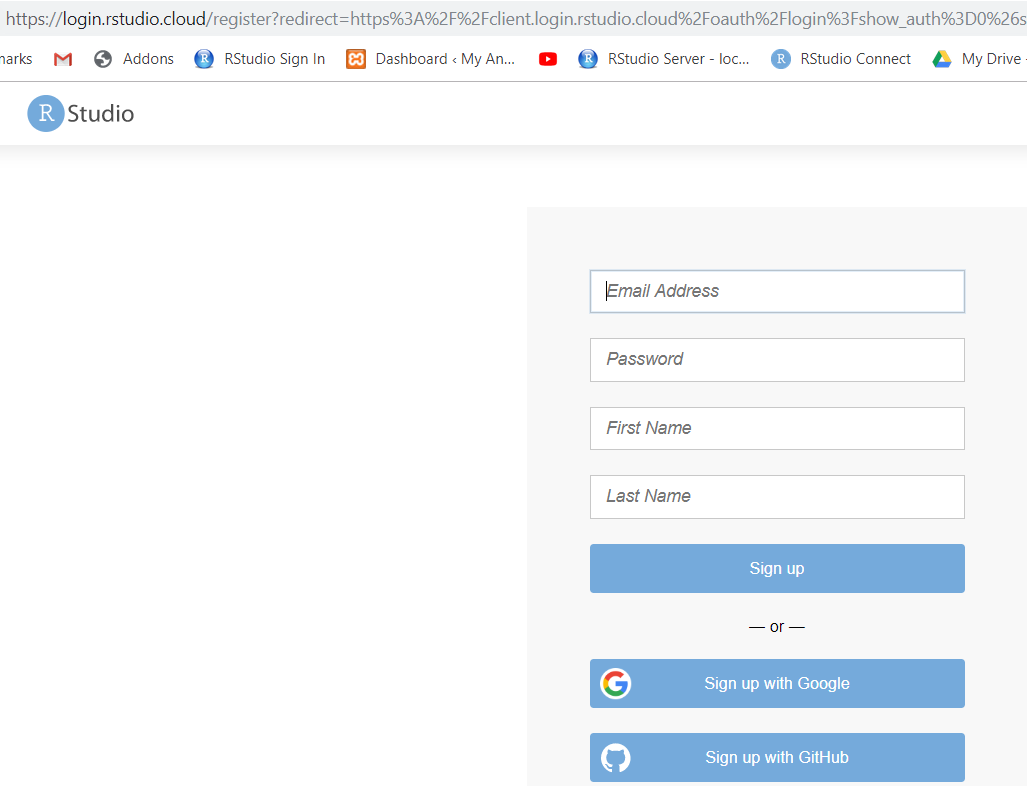
\includegraphics{cloud2.PNG}
\caption{RStudio Cloud Registration}
\end{figure}

\hypertarget{point-and-click-r-gui}{%
\section{Point and click R GUI}\label{point-and-click-r-gui}}

There are a number of GUI versions of R also known as R GUI. The interface resembles a popular statistical software SPSS\index{SPSS}. For example

\begin{itemize}
\tightlist
\item
  Bluesky statistics\index{Bluesky statistics} \url{https://www.blueskystatistics.com/}
\item
  JAMOVI\index{jamovi} - \url{https://www.jamovi.org/}
\end{itemize}

This is the \textbf{Bluesky statistics} software

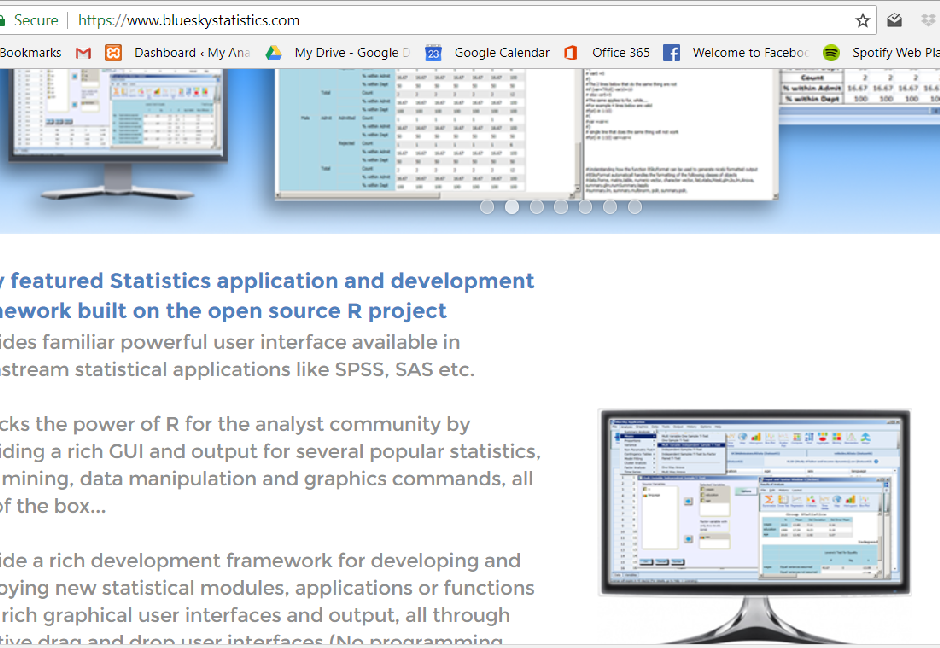
\includegraphics{bluesky.PNG}{]}

And this is \textbf{jamovi} software

\begin{figure}
\centering
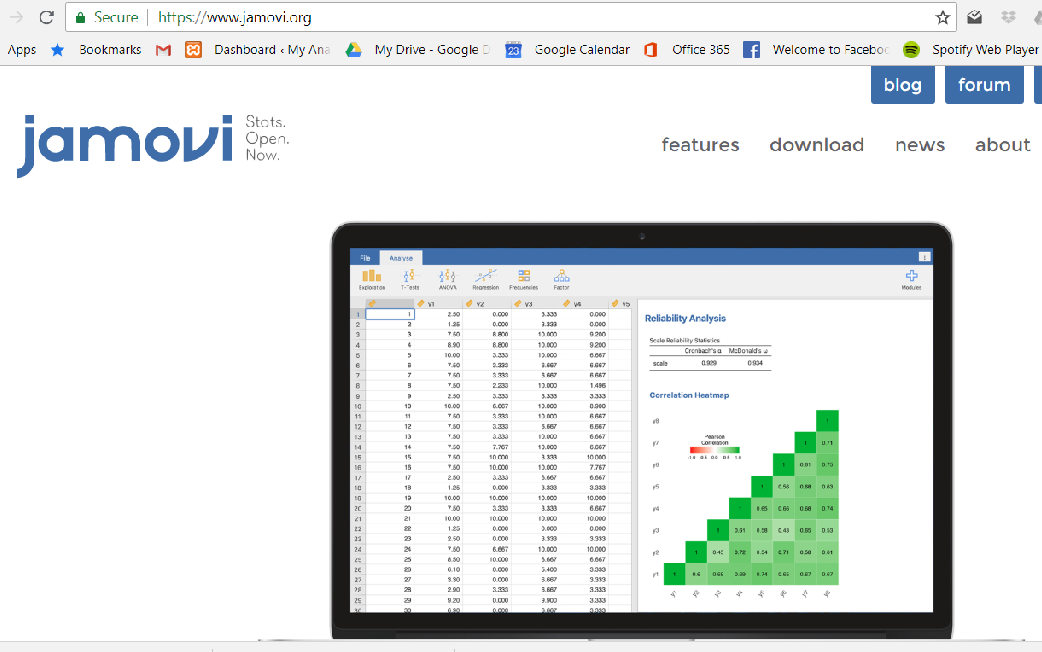
\includegraphics{jamovi.PNG}
\caption{jamovi software}
\end{figure}

jamovi\index{jamovi} is an interesting software. It is a new ``3rd generation'' statistical spreadsheet. It is designed from the ground up to be easy to use, it is a compelling alternative to costly statistical products such as SPSS\index{SPSS} and SAS\index{SAS}. jamovi\index{jamovi} is built on top of the R statistical language, giving you access to the best the statistics community has to offer. jamovi\index{jamovi} will always be free and open because jamovi\index{jamovi} is made by the scientific community, for the scientific community.

\hypertarget{rstudio-server}{%
\section{\texorpdfstring{RStudio Server\index{RStudio server}}{RStudio Server}}\label{rstudio-server}}

You can run R and RStudio\index{RStudio} on the server. To do this you have to install RStudio Workbench\index{RStudio workbench}. Previously, R Studio Workbench was known as RStudio Server\index{RStudio server}. By using RStudio Server\index{RStudio server}, R users can perform analysis on the server. Using RStudio server\index{RStudio server} can give you a taste of cloud data analysis.

There are two versions of RStudio server\index{RStudio server}:

\begin{itemize}
\tightlist
\item
  RStudio Server\index{RStudio server}: This is the Open Source edition
\item
  RStudio Workbench\index{RStudio workbench}: This is the Professional edition.
\end{itemize}

At our medical school. we have RStudio Server Professional Edition (\textbf{courtesy of} RStudio, of course) running on our server here \url{https://healthdata.usm.my/rstudio/auth-sign-in}

\hypertarget{installing-r-and-rstudio-on-your-local-machine}{%
\section{\texorpdfstring{Installing R and RStudio\index{RStudio} on Your Local Machine}{Installing R and RStudio on Your Local Machine}}\label{installing-r-and-rstudio-on-your-local-machine}}

To install R on your local machine, you have to have \textbf{Admin Right} to your machine. We recommend that you install

\begin{itemize}
\tightlist
\item
  \textbf{R} first,
\item
  then \textbf{RStudio}
\end{itemize}

\hypertarget{installing-r}{%
\subsection{Installing R}\label{installing-r}}

Though you can use the native R software (that you just installed) to run R codes, we highly encourage you to use RStudio Integrated Desktop Environment (IDE)\index{RStudio IDE}.

We will show this step by step. First, let us install R on your machine. To install R, go to \href{https://cran.r-project.org/}{cran}. Then choose the R version that's correct for your machine OS. For example, for Windows OS the link is \url{https://cran.r-project.org/bin/windows/base/R-4.2.1-win.exe}. And for Mac OS, the download link is \url{https://cran.r-project.org/bin/macosx/base/R-4.2.1.pkg}. Similarly, if you are using Linux, follow the steps as listed before.

\begin{figure}
\centering
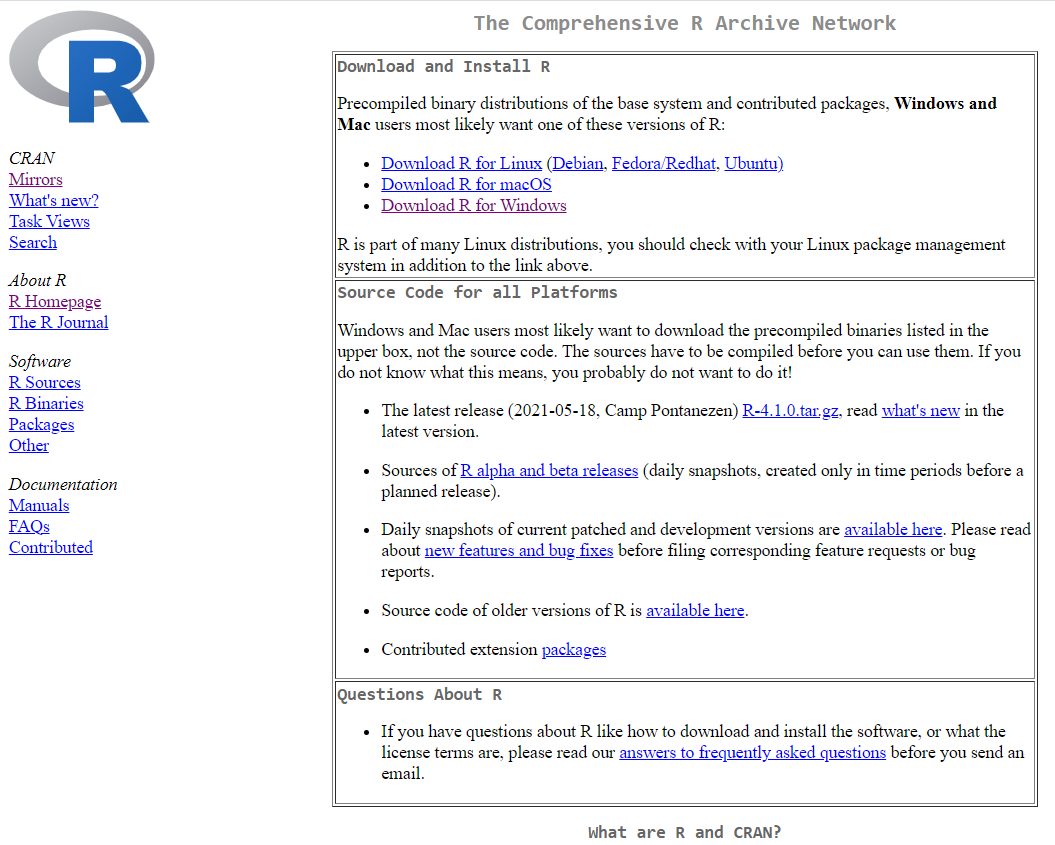
\includegraphics{cran.PNG}
\caption{CRAN website}
\end{figure}

It is always recommended that you install the latest version of R. During this writing, the latest version is R version 4.2.1 known as Funny-Looking Kid version that was released on 2022/06/23. You can have multiple R version on the same local machines. So you do not need to uninstall the old R version in order to install a new R version.

\hypertarget{installing-rstudio-ide}{%
\subsection{\texorpdfstring{Installing RStudio IDE\index{RStudio IDE}}{Installing RStudio IDE}}\label{installing-rstudio-ide}}

Now, to install RStudio IDE\index{RStudio IDE}, go here \url{https://www.rstudio.com/products/rstudio/download/\#download}. Choose the supported platforms correct for your machine OS. The size of download will be around 90-110 MB.

\begin{figure}
\centering

\includegraphics{rstudio2.PNG}
\caption{RStudio website}
\end{figure}

\hypertarget{checking-r-and-rstudio-installations}{%
\subsection{\texorpdfstring{Checking R and RStudio\index{RStudio} Installations}{Checking R and RStudio Installations}}\label{checking-r-and-rstudio-installations}}

Now, we assume you have installed both R and RStudio\index{RStudio}. To make sure they work perfectly (or at least for the first time), check:

\begin{itemize}
\tightlist
\item
  Does your machine can load R? Depending on your OS, go and start R.\\
\item
  what version of R do you have? When R loads, look for the version of R.
\item
  Do you have RStudio\index{RStudio}? Depending on your OS, go and start RStudio\index{RStudio}.
\item
  what version of RStudio\index{RStudio} do you have? When RStudio\index{RStudio} loads, look for the version of R. If you have multiple R version, you can choose the R version of your choice by going to \textbf{Tools} then \textbf{Global Options} then \textbf{General}
\item
  Do you need to update R and RStudio\index{RStudio}? By knowing the versions of R and RStudio\index{RStudio}, now you know if you need to update both or one of them.
\end{itemize}

\hypertarget{installation-of-miktex-texlive-and-mactex}{%
\subsection{Installation of MiKTeX, TeXLive and MacTex}\label{installation-of-miktex-texlive-and-mactex}}

It is necessary to install Latex editor if you want to convert the outputs you generated in R into PDF format. But if you do not need to produce PDF document, then you do not have to install it.

Based on experience, as you go along, you may find it is very attractive to convert your analysis into PDF document. And because of that, you need to install the Latex editor.


\includegraphics{rmarkdown.PNG}{]}

This is MiKTeX, for Window OS

\begin{figure}
\centering
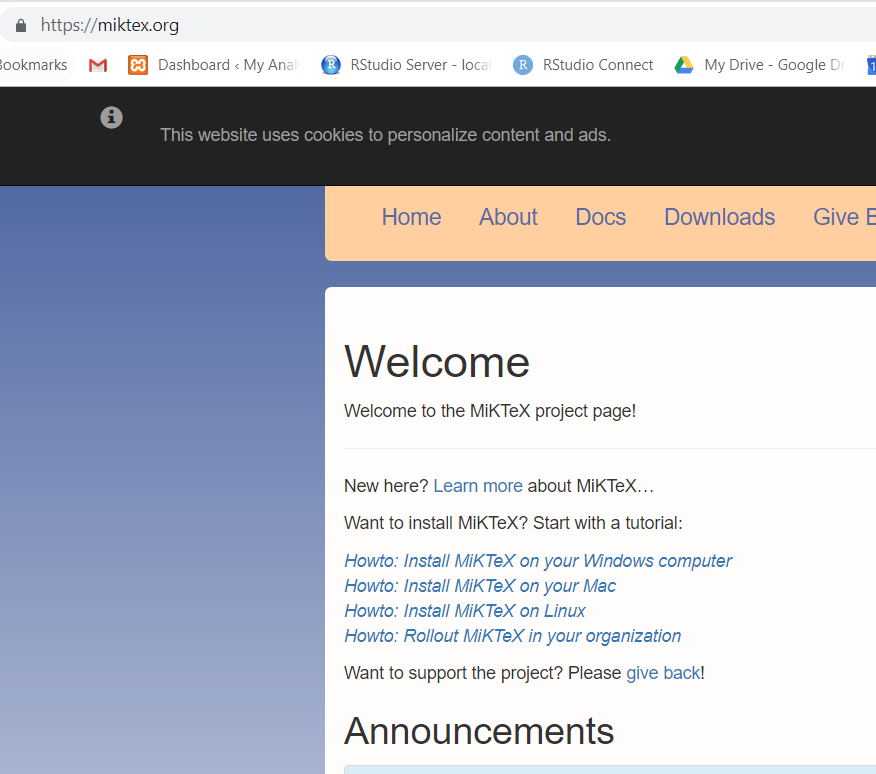
\includegraphics{miktex.PNG}
\caption{MikTeX webpage}
\end{figure}

And this is MacTeX, for Mac OS

\begin{figure}
\centering

\includegraphics{mactex.PNG}
\caption{MacTeX webpage}
\end{figure}

\hypertarget{starting-your-rstudio}{%
\section{\texorpdfstring{Starting your RStudio\index{RStudio}}{Starting your RStudio}}\label{starting-your-rstudio}}

You can either login to RStudio Cloud\index{RStudio cloud} and automatically see the RStudio interface OR you can start RStudio\index{RStudio} on your local machine by loading it. Remember, to login to RStudio Cloud\index{RStudio cloud}, go to \url{https://rstudio.cloud}. You will be asked for your username and password.

Click this link \url{https://rstudio.cloud/spaces/156361/join?access_code=WtlSxNuTm\%2Fz7E\%2BLb\%2FW2XnOw480\%2BBTmL4B\%2FqjYRIg}

\begin{figure}
\centering
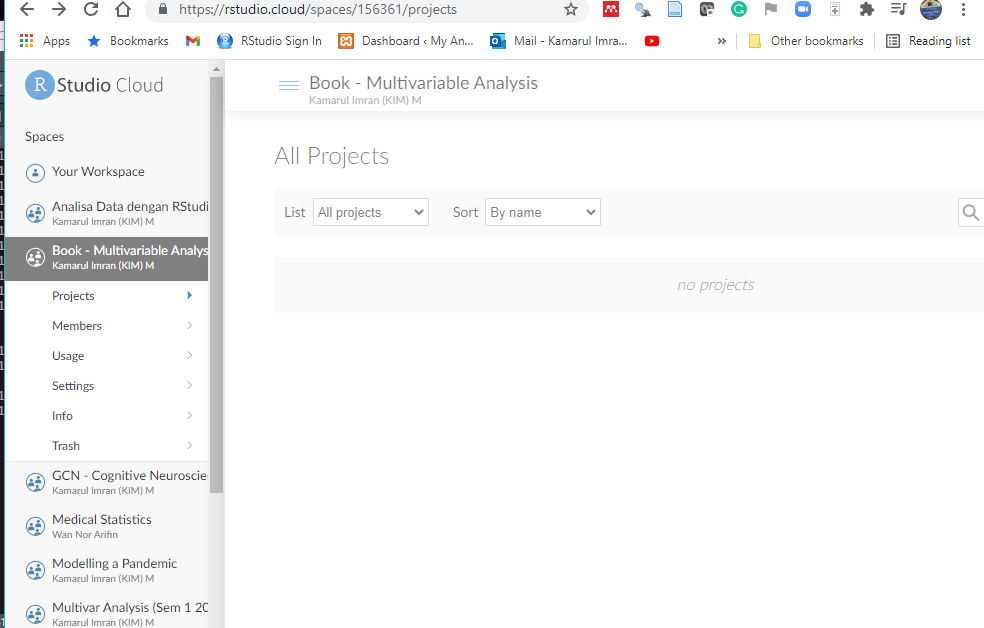
\includegraphics{book_rstudio_cloud.PNG}
\caption{RStudio Cloud space for this book}
\end{figure}

To start R on your machine, and if you are using Windows, find the RStudio\index{RStudio} program in your start bar in your machine. And start it. You will see an interface like below. This is definitely different with what you see on your screen because I am using the Vibrant Ink Theme. To choose the theme of your choice, click \textbf{Global Options} then, click \textbf{Apperance}. There are a number of themes available for you to choose.

\begin{figure}
\centering
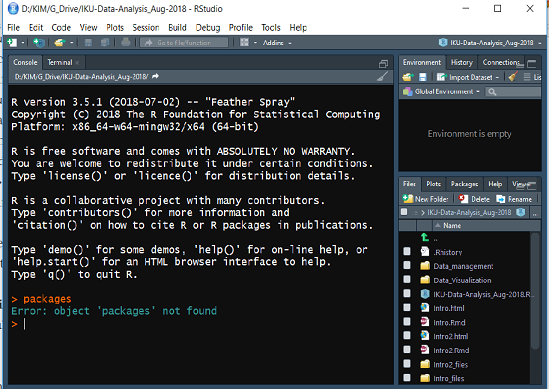
\includegraphics{rstudio.PNG}
\caption{Rstudio Interface with Vibrant Ink theme}
\end{figure}

What you see on RStudio\index{RStudio} now? You should see three panes if you start RStudio\index{RStudio} for the first time or four panes if you have used RStudio\index{RStudio} before.

\begin{figure}
\centering
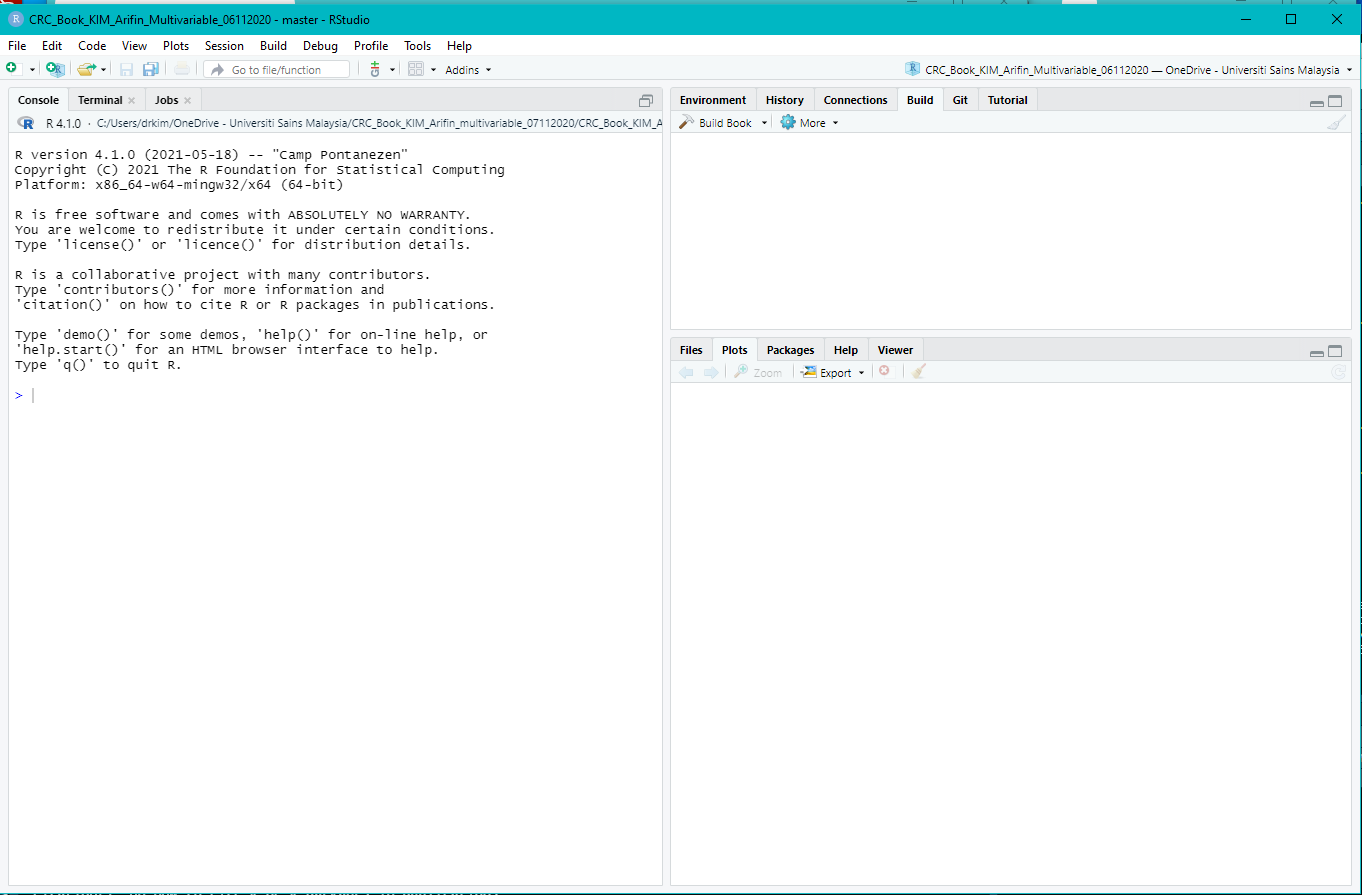
\includegraphics{rstudio_def.PNG}
\caption{RStudio Panes}
\end{figure}

\hypertarget{console-tab}{%
\subsection{Console tab}\label{console-tab}}

In Console tab, this is where we will see most of the results generated from codes in RStudio\index{RStudio}.

\begin{figure}
\centering
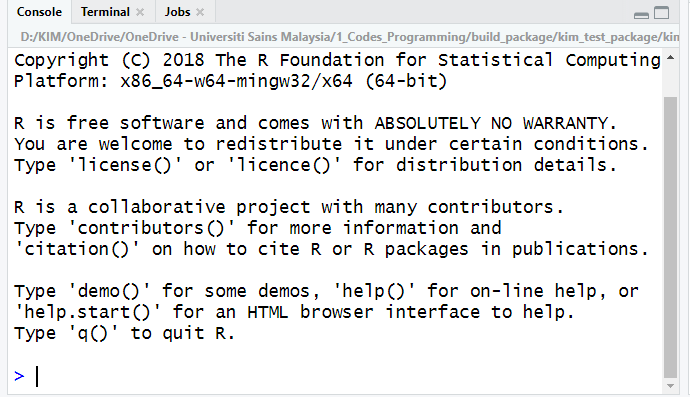
\includegraphics{console.PNG}
\caption{Console Pane}
\end{figure}

\hypertarget{files-plots-packages-help-and-viewer-pane}{%
\subsection{\texorpdfstring{Files, Plots, Packages\index{Packages}, Help and Viewer Pane}{Files, Plots, Packages, Help and Viewer Pane}}\label{files-plots-packages-help-and-viewer-pane}}

In this console, you will see

\begin{itemize}
\tightlist
\item
  List of objects (Remember, R is an object-oriented-programming or oop)
\item
  R files, datasets, tables, list etc
\end{itemize}

\begin{figure}
\centering
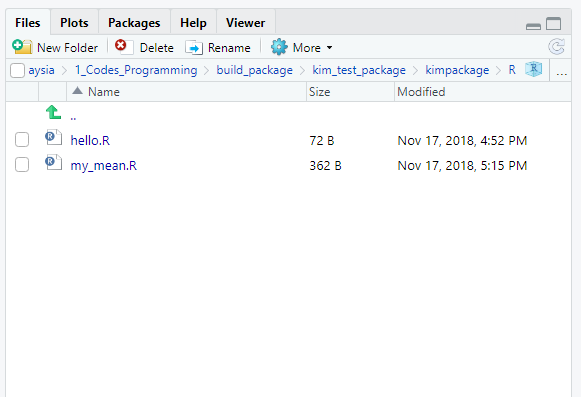
\includegraphics{files.PNG}
\caption{File, Plots and Viewer Pane}
\end{figure}

\hypertarget{environment-history-connection-and-build-pane}{%
\subsection{Environment, History, Connection and Build Pane}\label{environment-history-connection-and-build-pane}}

In the environment, history, connection and build pane, you will see this

\begin{figure}
\centering
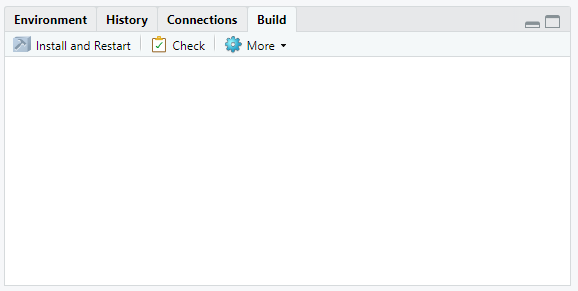
\includegraphics{envir.PNG}
\caption{Environment Pane}
\end{figure}

\hypertarget{source-pane}{%
\subsection{Source Pane}\label{source-pane}}

In the Source pane, you can create R files and write your R codes

\begin{figure}
\centering
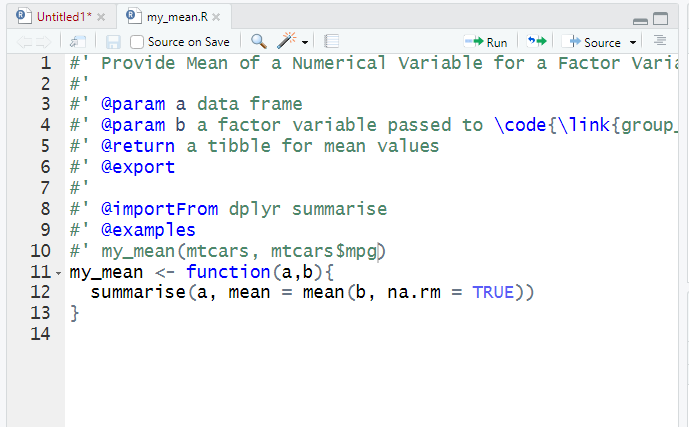
\includegraphics{source.PNG}
\caption{Source Pane}
\end{figure}

\hypertarget{r-scripts-and-r-packages}{%
\chapter{\texorpdfstring{R Scripts\index{R script} and R Packages\index{Packages}}{R Scripts and R Packages}}\label{r-scripts-and-r-packages}}

\hypertarget{introduction}{%
\section{Introduction}\label{introduction}}

\hypertarget{objectives-1}{%
\section{Objectives}\label{objectives-1}}

In this chapter, we would like to achieve these objectives:

\begin{itemize}
\tightlist
\item
\item
\item
\end{itemize}

\hypertarget{open-a-new-r-script}{%
\section{\texorpdfstring{Open a new R script\index{R script}}{Open a new R script}}\label{open-a-new-r-script}}

For beginner, you may start by writing some simple codes. Since these codes are written in R language, we call these codes as R scripts\index{R script}. To do this, go to \textbf{File}, then click \textbf{R Script}

\begin{itemize}
\tightlist
\item
  File -\textgreater{} R Script\index{R script}
\item
  In Window OS, CTRL-SHIFT-N
\end{itemize}

\begin{figure}
\centering
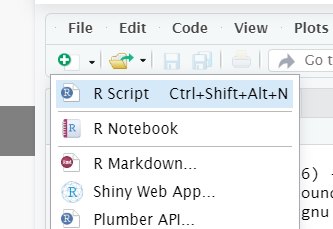
\includegraphics{Rscript.PNG}
\caption{New R Script}
\end{figure}

\hypertarget{our-first-r-script}{%
\subsection{\texorpdfstring{Our first R script\index{R script}}{Our first R script}}\label{our-first-r-script}}

Let us write our very first R codes inside an R script\index{R script}.

\begin{itemize}
\tightlist
\item
  In Line 1, type \texttt{2\ +\ 3}
\item
  click CTRL-ENTER or CMD-ENTER
\item
  see the outputs in the Console Pane
\end{itemize}

\begin{Shaded}
\begin{Highlighting}[]
\DecValTok{2} \SpecialCharTok{+} \DecValTok{3}
\end{Highlighting}
\end{Shaded}

\begin{verbatim}
## [1] 5
\end{verbatim}

After writing your codes inside the R script\index{R script}, you can save the R script\index{R script} file. This will allow you to open it up again to continue your work.

And to save R script\index{R script}, go to

\begin{itemize}
\tightlist
\item
  File -\textgreater{}
\item
  Save As -\textgreater{}
\item
  Choose folder -\textgreater{}\\
\item
  Name the file
\end{itemize}

Now, types this to check the version of R

\begin{Shaded}
\begin{Highlighting}[]
\NormalTok{version[}\DecValTok{6}\SpecialCharTok{:}\DecValTok{7}\NormalTok{]}
\end{Highlighting}
\end{Shaded}

\begin{verbatim}
##       _  
## major 3  
## minor 6.3
\end{verbatim}

The current version for R is 3, 6.3

If you lower version, then you want to upgrade. To upgrade

\begin{itemize}
\tightlist
\item
  for Windows, you can use \textbf{installr} package
\item
  for Mac OS, you can use some functions
\end{itemize}

More info here \url{https://www.linkedin.com/pulse/3-methods-update-r-rstudio-windows-mac-woratana-ngarmtrakulchol/}

\hypertarget{function-argument-and-parameters}{%
\subsection{Function, Argument and Parameters}\label{function-argument-and-parameters}}

R codes contain

\begin{itemize}
\tightlist
\item
  function
\item
  argument
\item
  parameters
\end{itemize}

\begin{verbatim}
f <- function(<arguments>) {
## Do something interesting
}
\end{verbatim}

For example, for the function \texttt{lm()} to estimate parameters for linear regression model

\begin{Shaded}
\begin{Highlighting}[]
\FunctionTok{args}\NormalTok{(lm)}
\end{Highlighting}
\end{Shaded}

\begin{verbatim}
## function (formula, data, subset, weights, na.action, method = "qr", 
##     model = TRUE, x = FALSE, y = FALSE, qr = TRUE, singular.ok = TRUE, 
##     contrasts = NULL, offset, ...) 
## NULL
\end{verbatim}

For example:

\begin{Shaded}
\begin{Highlighting}[]
\FunctionTok{lm}\NormalTok{(weight }\SpecialCharTok{\textasciitilde{}}\NormalTok{ Time, }\AttributeTok{data =}\NormalTok{ ChickWeight)}
\end{Highlighting}
\end{Shaded}

\begin{verbatim}
## 
## Call:
## lm(formula = weight ~ Time, data = ChickWeight)
## 
## Coefficients:
## (Intercept)         Time  
##      27.467        8.803
\end{verbatim}

\hypertarget{need-more-help}{%
\subsection{Need more help?}\label{need-more-help}}

Then type the ? before the function

\begin{Shaded}
\begin{Highlighting}[]
\NormalTok{?lm}
\end{Highlighting}
\end{Shaded}

See what will be displayed in Help Pane\index{Help pane}

\begin{figure}
\centering
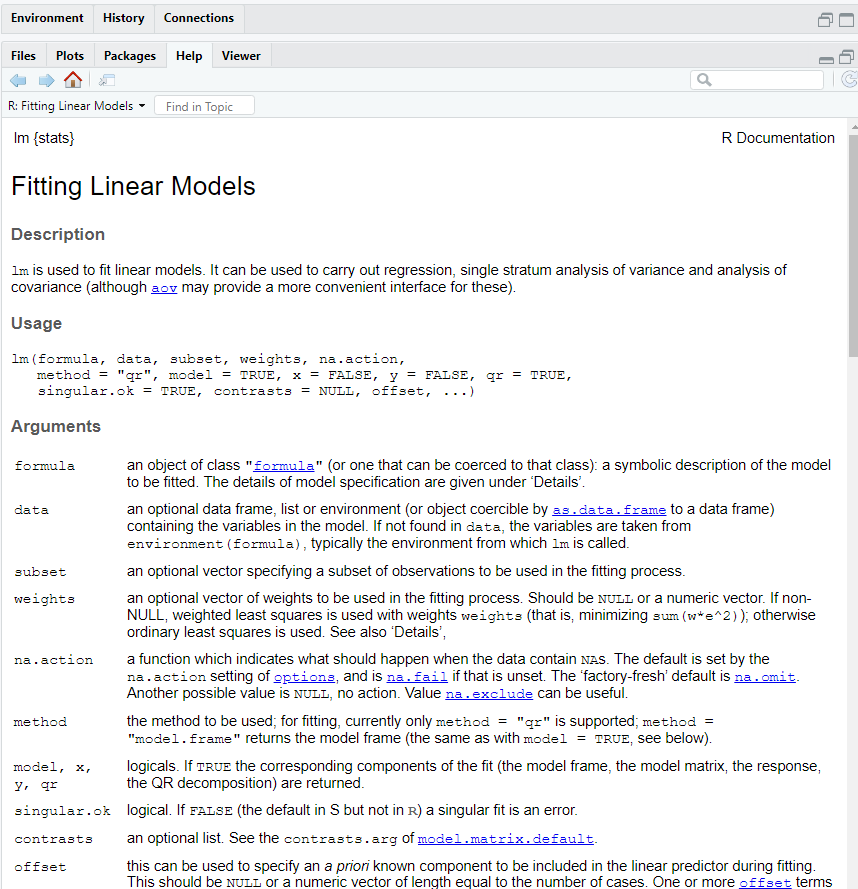
\includegraphics{lm.PNG}
\caption{Help Pane}
\end{figure}

\hypertarget{packages}{%
\section{\texorpdfstring{Packages\index{Packages}}{Packages}}\label{packages}}

R is a programming language. And R software runs on packages\index{Packages}. R packages\index{Packages} are collections of functions and data sets developed by the community. They increase the power of R by improving existing base R codes and functions, or by adding new ones.

A package is a suitable way to organize your own work and, if you want to, share it with others. Typically, a package will include code (not only R code!), documentation for the package and the functions inside, some tests to check everything works as it should, and data sets.

Ypu can read more about R packages\index{Packages} here \url{https://www.datacamp.com/community/tutorials/r-packages-guide}

\hypertarget{packages-on-cran}{%
\subsection{\texorpdfstring{Packages\index{Packages} on CRAN\index{Packages}}{Packages on CRAN}}\label{packages-on-cran}}

\url{https://cran.r-project.org/}

\begin{itemize}
\tightlist
\item
  At the time of writing, the CRAN\index{CRAN} package repository features 12784 packages\index{Packages}
\item
  Cran Task Views\index{Task Views}
\end{itemize}

\begin{figure}
\centering
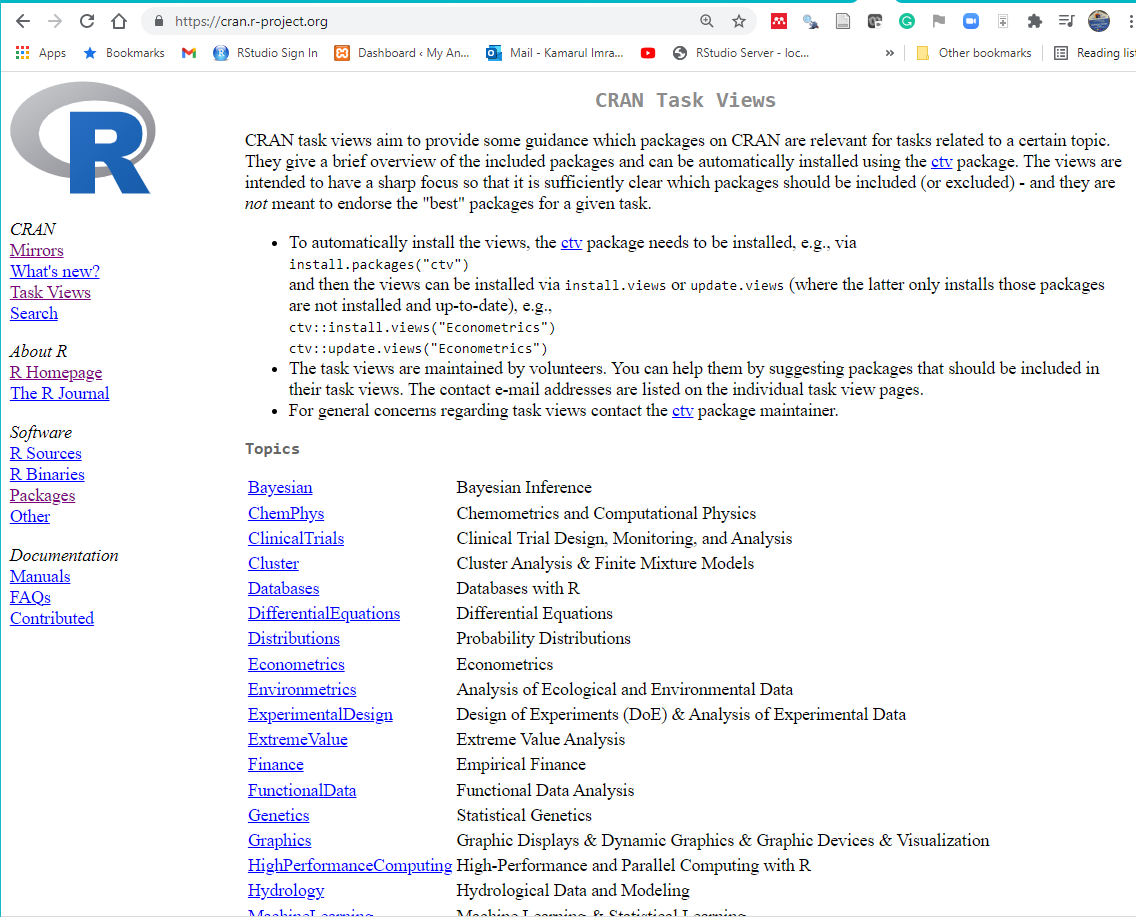
\includegraphics{packages.PNG}
\caption{Task Views}
\end{figure}

CRAN task views\index{Task Views} aim to provide some guidance which packages\index{Packages} on CRAN\index{CRAN} are relevant for tasks related to a certain topic. They give a brief overview of the included packages\index{Packages} and can be automatically installed using the \textbf{ctv} package. The views are intended to have a sharp focus so that it is sufficiently clear which packages\index{Packages} should be included (or excluded) and they are not meant to endorse the ``best'' packages\index{Packages} for a given task.

\hypertarget{check-if-the-package-you-need-is-available-in-your-r-library}{%
\subsection{Check if the package you need is available in your R library}\label{check-if-the-package-you-need-is-available-in-your-r-library}}

Type this inside your R console

\begin{Shaded}
\begin{Highlighting}[]
\FunctionTok{library}\NormalTok{(tidyverse)}
\end{Highlighting}
\end{Shaded}

\begin{verbatim}
## -- Attaching packages --------------------------------------- tidyverse 1.3.2 --
## v ggplot2 3.3.6     v purrr   0.3.4
## v tibble  3.1.8     v dplyr   1.0.9
## v tidyr   1.2.0     v stringr 1.4.0
## v readr   2.1.2     v forcats 0.5.1
## -- Conflicts ------------------------------------------ tidyverse_conflicts() --
## x dplyr::filter() masks stats::filter()
## x dplyr::lag()    masks stats::lag()
\end{verbatim}

You should not receive any error message. If you have not installed the package, you will receive and error message. And it tells you that the package is not available in your R. By default the package is stored in the R folder in your My Document or HOME directory

\begin{Shaded}
\begin{Highlighting}[]
\FunctionTok{.libPaths}\NormalTok{()}
\end{Highlighting}
\end{Shaded}

\begin{verbatim}
## [1] "/home/wnarifin/R/x86_64-pc-linux-gnu-library/3.6"
## [2] "/usr/local/lib/R/site-library"                   
## [3] "/usr/lib/R/site-library"                         
## [4] "/usr/lib/R/library"
\end{verbatim}

\hypertarget{install-an-r-package}{%
\subsection{\texorpdfstring{Install an R package\index{Packages}}{Install an R package}}\label{install-an-r-package}}

To install an R package\index{Packages}, there are two ways:

\begin{enumerate}
\def\labelenumi{\arabic{enumi}.}
\tightlist
\item
  you can type below (without the \# tag)
\end{enumerate}

\begin{Shaded}
\begin{Highlighting}[]
\CommentTok{\# install.packages(tidyverse, dependencies = TRUE)}
\end{Highlighting}
\end{Shaded}

\begin{enumerate}
\def\labelenumi{\arabic{enumi}.}
\setcounter{enumi}{1}
\tightlist
\item
  using the GUI\index{GUI}
\end{enumerate}

\begin{figure}
\centering
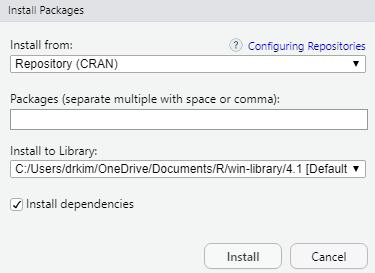
\includegraphics{tidyverse.png}
\caption{Packages pane}
\end{figure}

Now, type the package\index{Packages} you want to install. For example you want to install the \textbf{tidyverse}\index{tidyverse} package

\begin{figure}
\centering
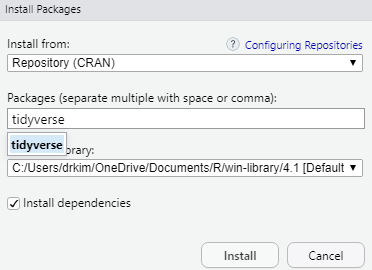
\includegraphics{tidyverse2.png}
\caption{Typing the package to install}
\end{figure}

And then click the \texttt{Install} button. And you need to have internet access to do this. You can also install packages\index{Packages} from:

\begin{itemize}
\tightlist
\item
  a zip file (from your machine or USB),
\item
  from github repository\index{GitHub repository}
\item
  other repository
\end{itemize}

\hypertarget{directory}{%
\section{Directory}\label{directory}}

Setting and knowing the R working directory\index{Working directory} is very important. Our working directory\index{Working directory} will contain the R codes, the R outputs, datasets or even resources or tutorials that can help us during in R project or during our R analysis/

The working directory\index{Working directory} is a just a folder. And the folder can contain many sub folders. We recommend that the folder contain the dataset (if you want to analyze your data locally) in addition to other R objects. R will store many other R objects created during each R session.

Type this to locate the working directiry:

\begin{Shaded}
\begin{Highlighting}[]
\FunctionTok{getwd}\NormalTok{()}
\end{Highlighting}
\end{Shaded}

\begin{verbatim}
## [1] "/home/wnarifin/Clouds/pCloud_Local/multivar_data_analysis"
\end{verbatim}

\hypertarget{starting-your-r-job}{%
\subsection{Starting your R job}\label{starting-your-r-job}}

There are 2 ways to start your job:

\begin{itemize}
\tightlist
\item
  create a new R project from RStudio IDE\index{RStudio IDE}. This is the method that we recommend.
\item
  setting your working directory using the \texttt{setwd()} function.
\end{itemize}

\hypertarget{create-new-r-project}{%
\subsection{\texorpdfstring{Create new R project\index{New project}}{Create new R project}}\label{create-new-r-project}}

We highly encourage users create a new R project. We can do this by

\begin{itemize}
\tightlist
\item
  Go to \texttt{File\ -\textgreater{}\ New\ Project}
\end{itemize}

{[}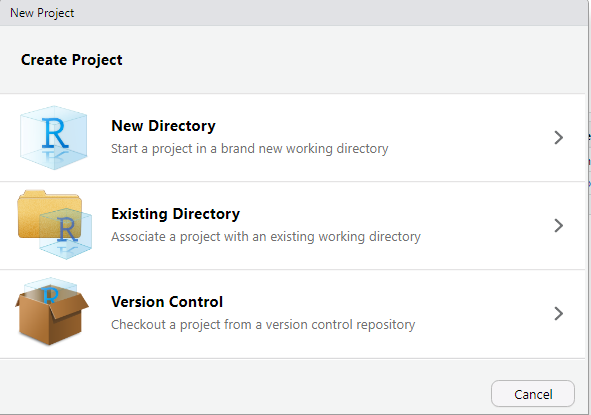
\includegraphics{new_proj.PNG}{]}

When you see project type, click New Project\index{New project}

\begin{figure}
\centering
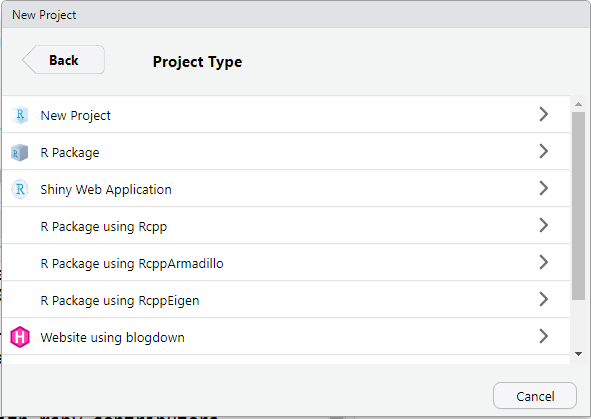
\includegraphics{new_proj2.PNG}
\caption{Project Type}
\end{figure}

\hypertarget{where-is-my-data}{%
\subsection{Where is my data?}\label{where-is-my-data}}

Many analysts use data stored in their local machine. R will read data and usually store this data in data frame format or class. When you read your data into RStudio\index{RStudio}, you will see the dataset in the environment pane. RStudio\index{RStudio} reads the original dataset and save in to the RAM (random access memory). SO you must know the size of your computer RAM. How much your RAM for your machine? The bigger the RAM, the larger R can read and store your data in the computer memory.

The data that is read (in memory) will disappear once you close RStudio\index{RStudio}. But the source dataset wil stay in its original location. This will not change your original data (so be happy!) unless you choose to save the dataframe in the memory and replace the original file. But we do not recommed you doing this.

\begin{figure}
\centering
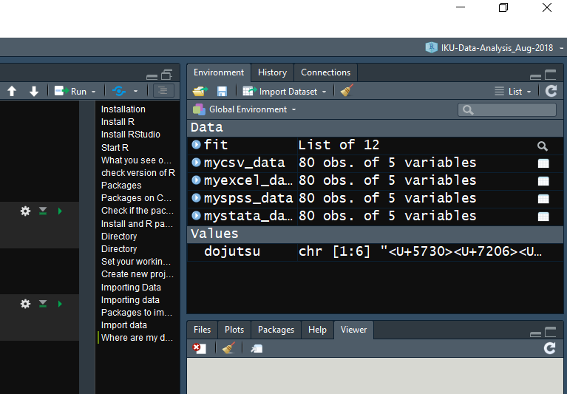
\includegraphics{mydata.PNG}
\caption{My Data}
\end{figure}

\hypertarget{upload-data-to-rstudio-cloud}{%
\section{\texorpdfstring{Upload data to RStudio Cloud\index{RStudio cloud}}{Upload data to RStudio Cloud}}\label{upload-data-to-rstudio-cloud}}

You have to upload data to RStudio Cloud\index{RStudio cloud} or link data to dropbox folder

\begin{figure}
\centering
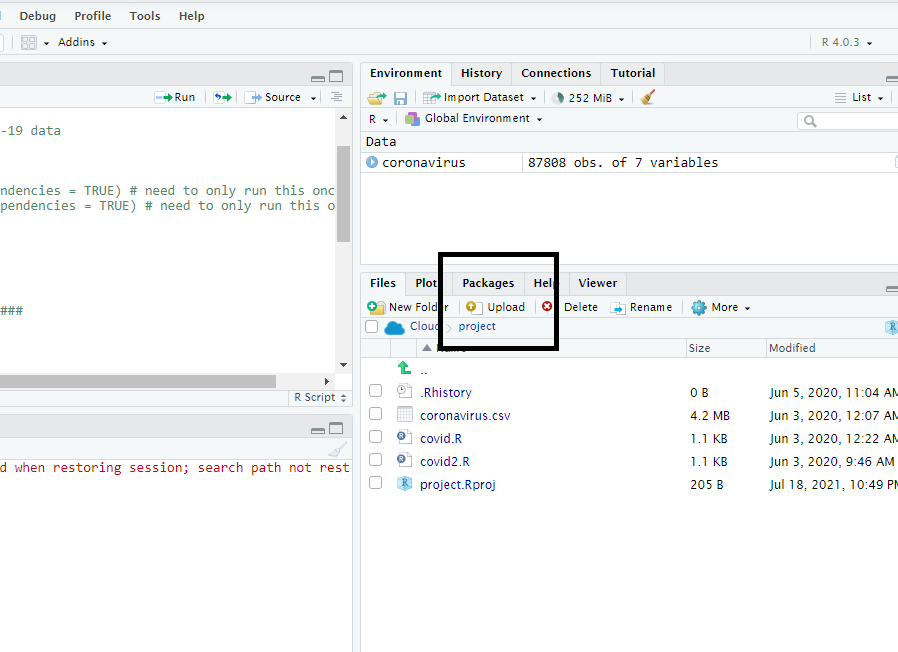
\includegraphics{upload_data.PNG}
\caption{Upload Data in RStudio Cloud}
\end{figure}

\hypertarget{more-resources-on-rstudio-cloud}{%
\section{\texorpdfstring{More resources on RStudio Cloud\index{RStudio cloud}}{More resources on RStudio Cloud}}\label{more-resources-on-rstudio-cloud}}

You can learn more about RStudio Cloud\index{RStudio cloud} here

\begin{itemize}
\item
  on YouTube : RStudio Cloud\index{RStudio cloud} for educationn \url{https://www.youtube.com/watch?v=PviVimazpz8}
\item
  YouTube: Working with R in Cloud \url{https://www.youtube.com/watch?v=SFpzr21Pavg}
\end{itemize}

\hypertarget{need-help}{%
\section{Need help?}\label{need-help}}

If you need help you can

\begin{itemize}
\tightlist
\item
  Type a question mark infront of a function
\end{itemize}

\begin{Shaded}
\begin{Highlighting}[]
\NormalTok{?plot}
\end{Highlighting}
\end{Shaded}

Other options are these:

\begin{itemize}
\tightlist
\item
  register and join RStudio Community here \url{https://community.rstudio.com/}
\item
  Ask questions on Stack Overflow \url{https://stackoverflow.com/}
\item
  Search for mailing list and subscribe to it
\item
  Books on R \url{https://bookdown.org/}
\end{itemize}

\hypertarget{bookdown}{%
\section{Bookdown}\label{bookdown}}

This webpage contains many useful books that use R codes \url{https://bookdown.org/}.

\begin{figure}
\centering

\includegraphics{bookdown.PNG}
\caption{Bookdown}
\end{figure}

\hypertarget{rstudio-project}{%
\chapter{RStudio Project}\label{rstudio-project}}

In this chapter, we will guide readers to have a similar folder and file structure. This will help readers to run the codes with minimal risk for errors. And we do this by creating RStudio Project.

From the RStudio Project webpage \url{https://support.rstudio.com/hc/en-us/articles/200526207-Using-RStudio-Projects} , it says that RStudio projects make it straightforward to divide your work into multiple contexts, each with their own working directory, workspace, history, and source documents.RStudio projects are associated with R working directories. You can create an RStudio project:

\begin{itemize}
\tightlist
\item
  on RStudio Cloud\index{RStudio cloud} or RStudio on your local machine
\item
  In a brand new directory
\item
  In an existing directory where you already have R code and data
\item
  By cloning a version control (Git or Subversion) repository
\end{itemize}

\hypertarget{objectives-2}{%
\section{Objectives}\label{objectives-2}}

The objectives of the chapters are

\begin{itemize}
\tightlist
\item
  to share the link for the dataset repository on GitHub\index{GitHub}
\item
  to teach readers to create a RStudio Cloud project based on the dataset repository on GitHub\index{GitHub}
\item
  to teach readers to create a RStudio project on local machine based on the dataset repository on GitHub\index{GitHub}
\end{itemize}

\hypertarget{dataset-repository-on-github}{%
\section{\texorpdfstring{Dataset repository on GitHub\index{GitHub}}{Dataset repository on GitHub}}\label{dataset-repository-on-github}}

We will use the our book repository on GitHub\index{GitHub}. The repository is \texttt{data-for-RMed}. To go to the repository, click on this link

\begin{figure}
\centering
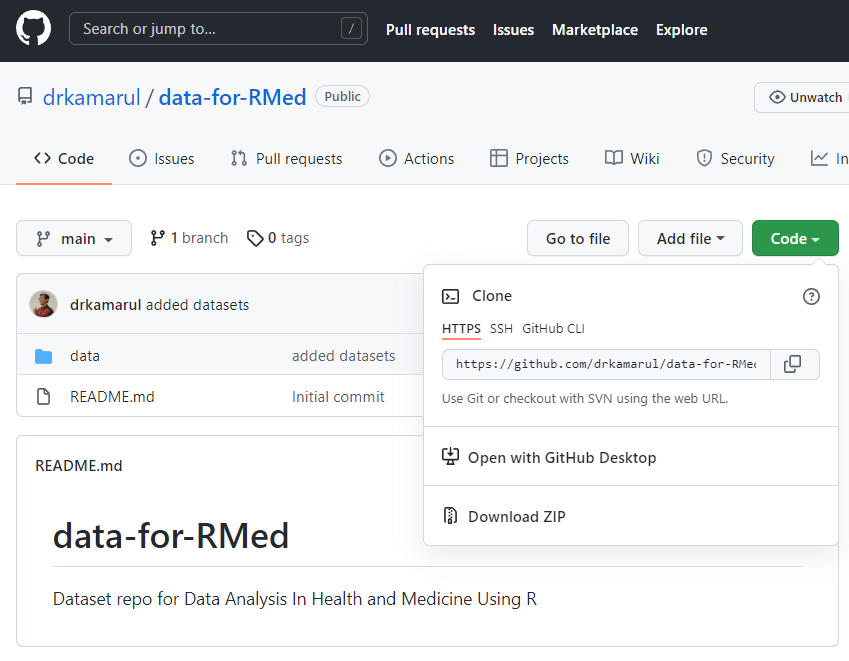
\includegraphics{5clonegit.png}
\caption{Dataset Repository on GitHub}
\end{figure}

\hypertarget{rstudio-project-on-rstudio-cloud}{%
\section{\texorpdfstring{RStudio project on RStudio Cloud\index{RStudio cloud}}{RStudio project on RStudio Cloud}}\label{rstudio-project-on-rstudio-cloud}}

Head to RStudio Cloud\index{RStudio cloud} page


\includegraphics{1login.png}
Login to RStudio Cloud\index{RStudio cloud} using your credentials

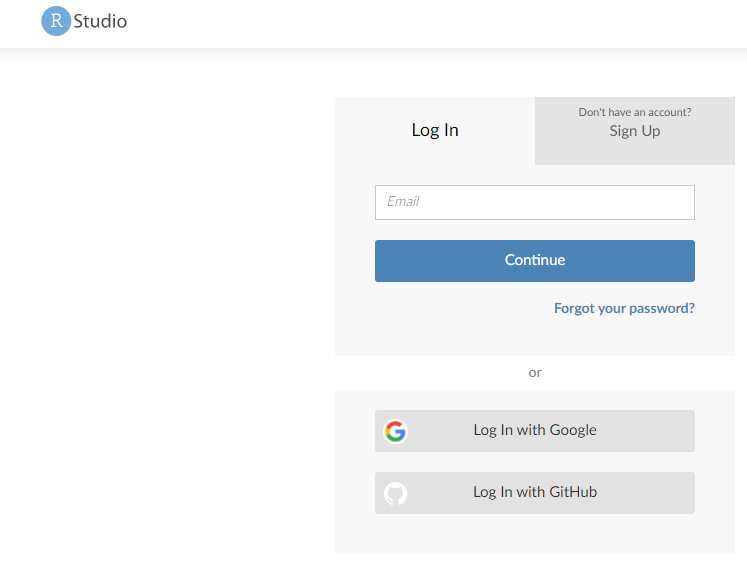
\includegraphics{2login.png}
Once inside your workspace, click New Project

\begin{figure}
\centering

\includegraphics{3newproject.png}
\caption{Rstudio Cloud, Workspace and New Project}
\end{figure}

And click on \texttt{New\ Project\ from\ Git\ Repository}\index{Git repository}

\begin{figure}
\centering
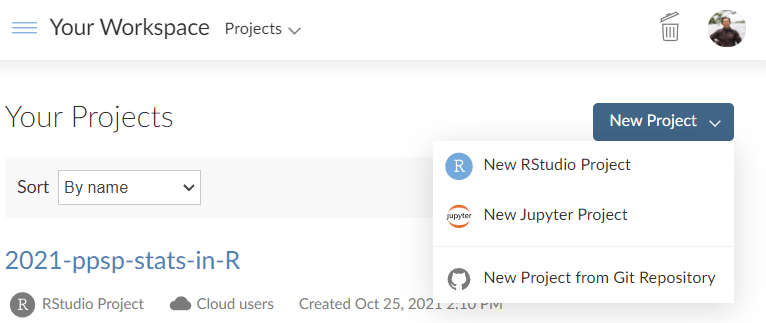
\includegraphics{4newprojectfromgit.png}
\caption{New Project from Git Repository}
\end{figure}

You will got back to our \texttt{data-for-RMed} repository on GitHub\index{GitHub}. And you will click on \texttt{Clone}\index{Clone} and click the copy button for HTTPS

\begin{figure}
\centering
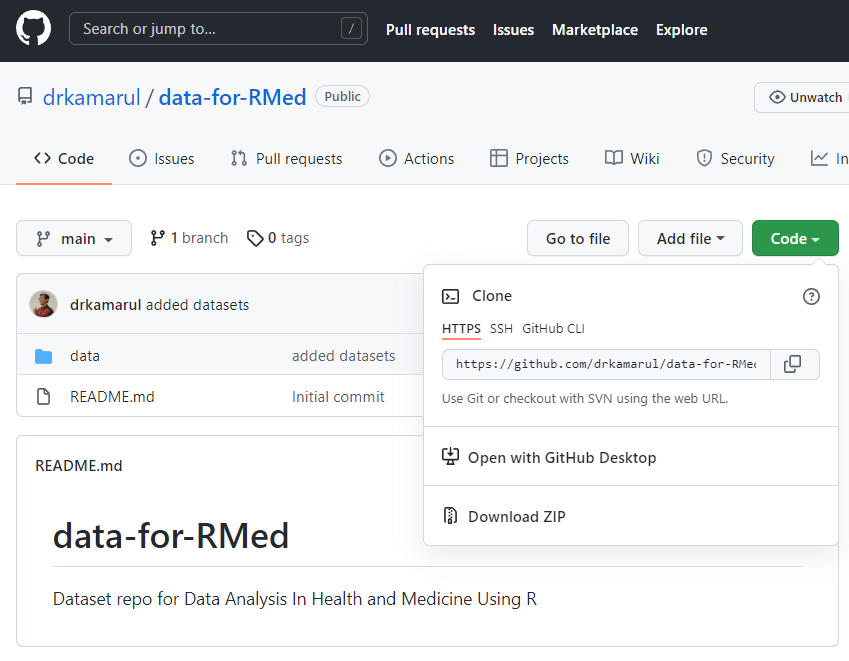
\includegraphics{5clonegit.png}
\caption{Clone Git Repository to RStudio Cloud}
\end{figure}

Next, we will clone\index{Clone} the repository on our RStudio Cloud\index{RStudio cloud}. This will ensure the file structure is the same with that of on the RStudio Cloud\index{RStudio cloud}. Following that, just click OK.

\begin{figure}
\centering
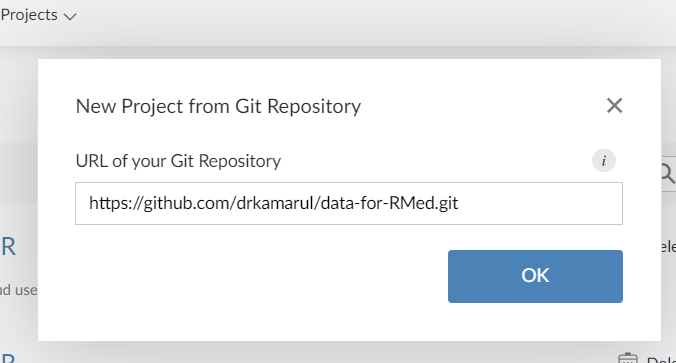
\includegraphics{6paste_url_git.png}
\caption{Clone the GitHub repository on RStudio Cloud project}
\end{figure}

A new Rstudio Cloud project will be created.

\begin{figure}
\centering
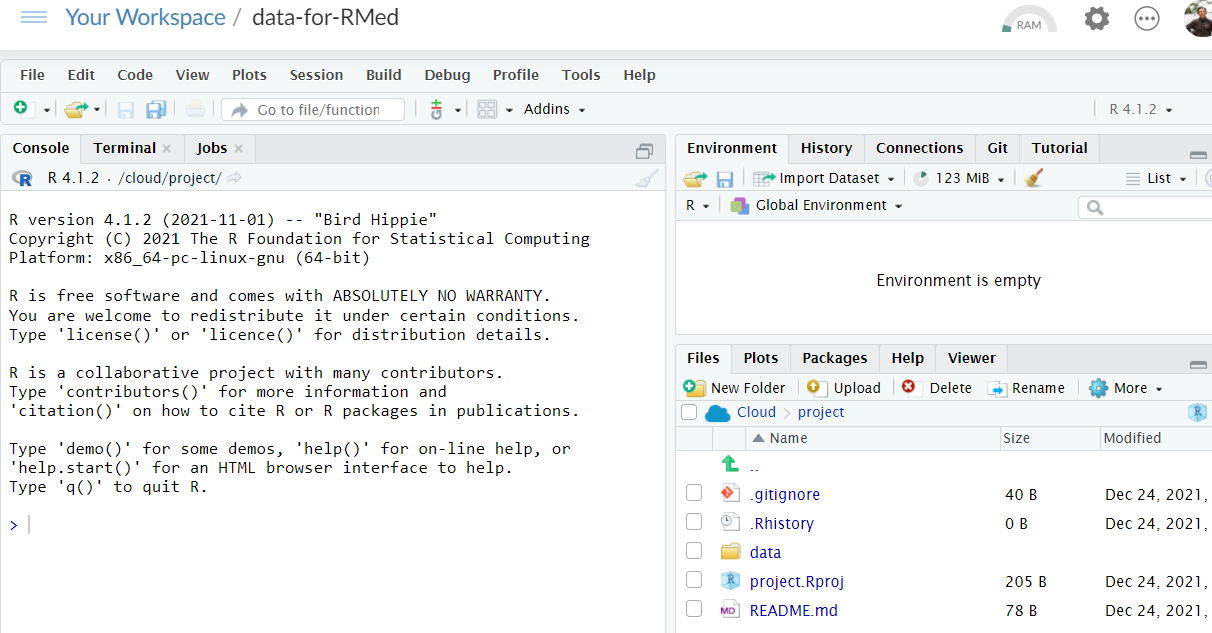
\includegraphics{7rstudiocloud.png}
\caption{A new RStudio Cloud Project}
\end{figure}

\hypertarget{rstudio-project-on-local-machine}{%
\section{RStudio project on local machine}\label{rstudio-project-on-local-machine}}

If you want to create a new project\index{New project} on your local machine using the same GitHub repository\index{GitHub repository}, then follow these steps.

First, open the RStudio.

\begin{figure}
\centering
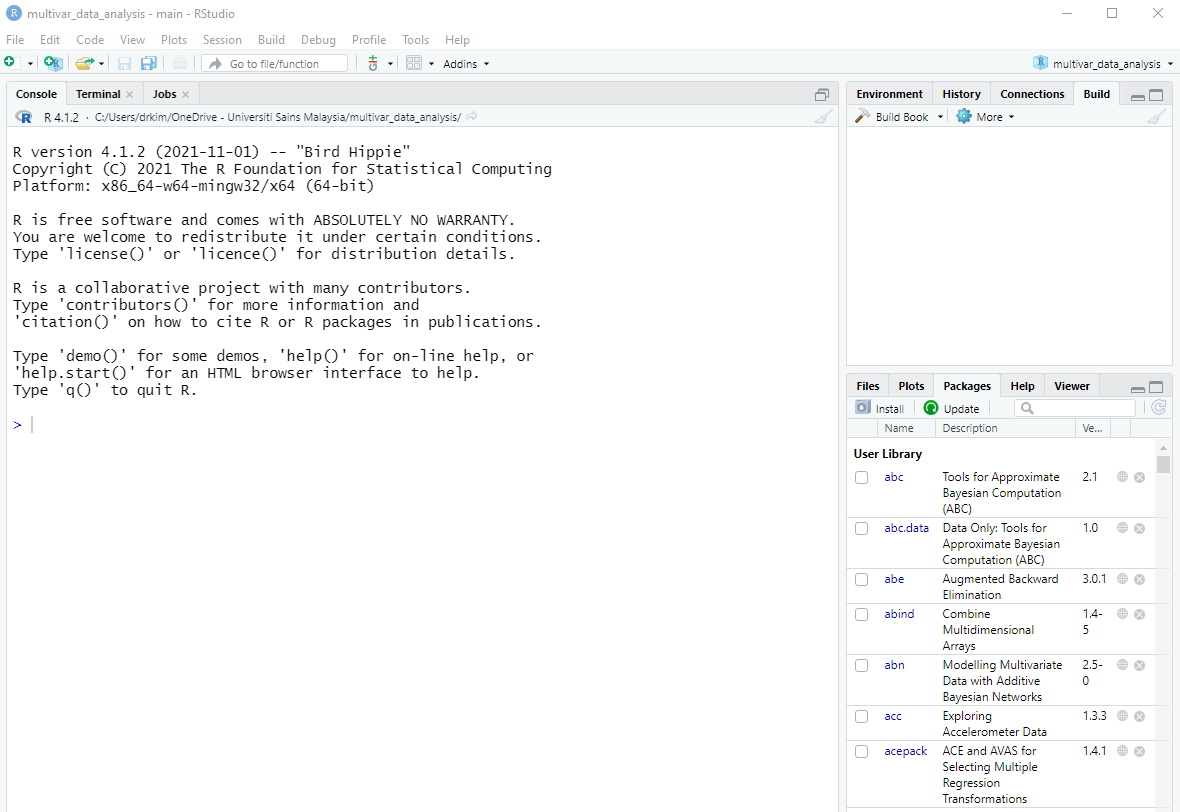
\includegraphics{11openrstudio.png}
\caption{RStudio on Your Machine}
\end{figure}

On the menu, click \texttt{File}, then click \texttt{New\ Project}

\begin{figure}
\centering
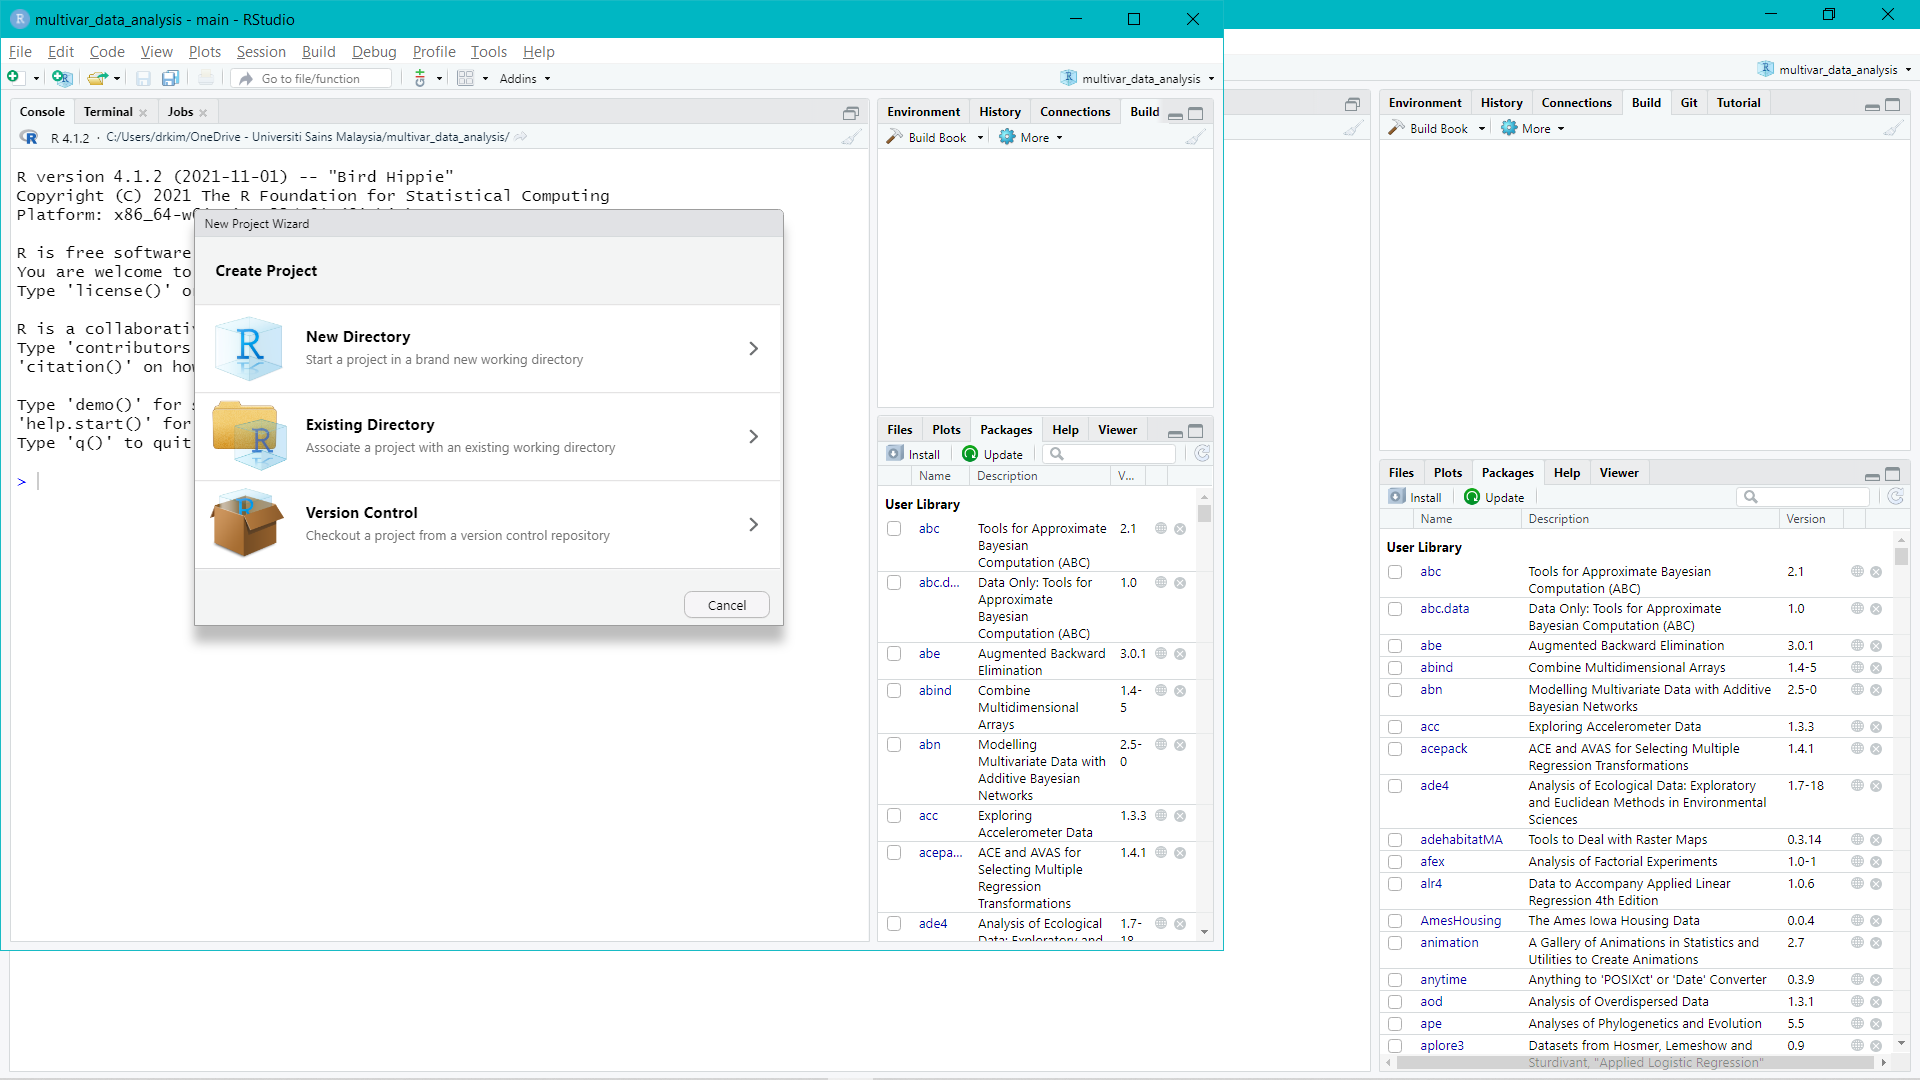
\includegraphics{12newproject.png}
\caption{New Project}
\end{figure}

Then click \texttt{Project} and then \texttt{Version\ Control}

\begin{figure}
\centering
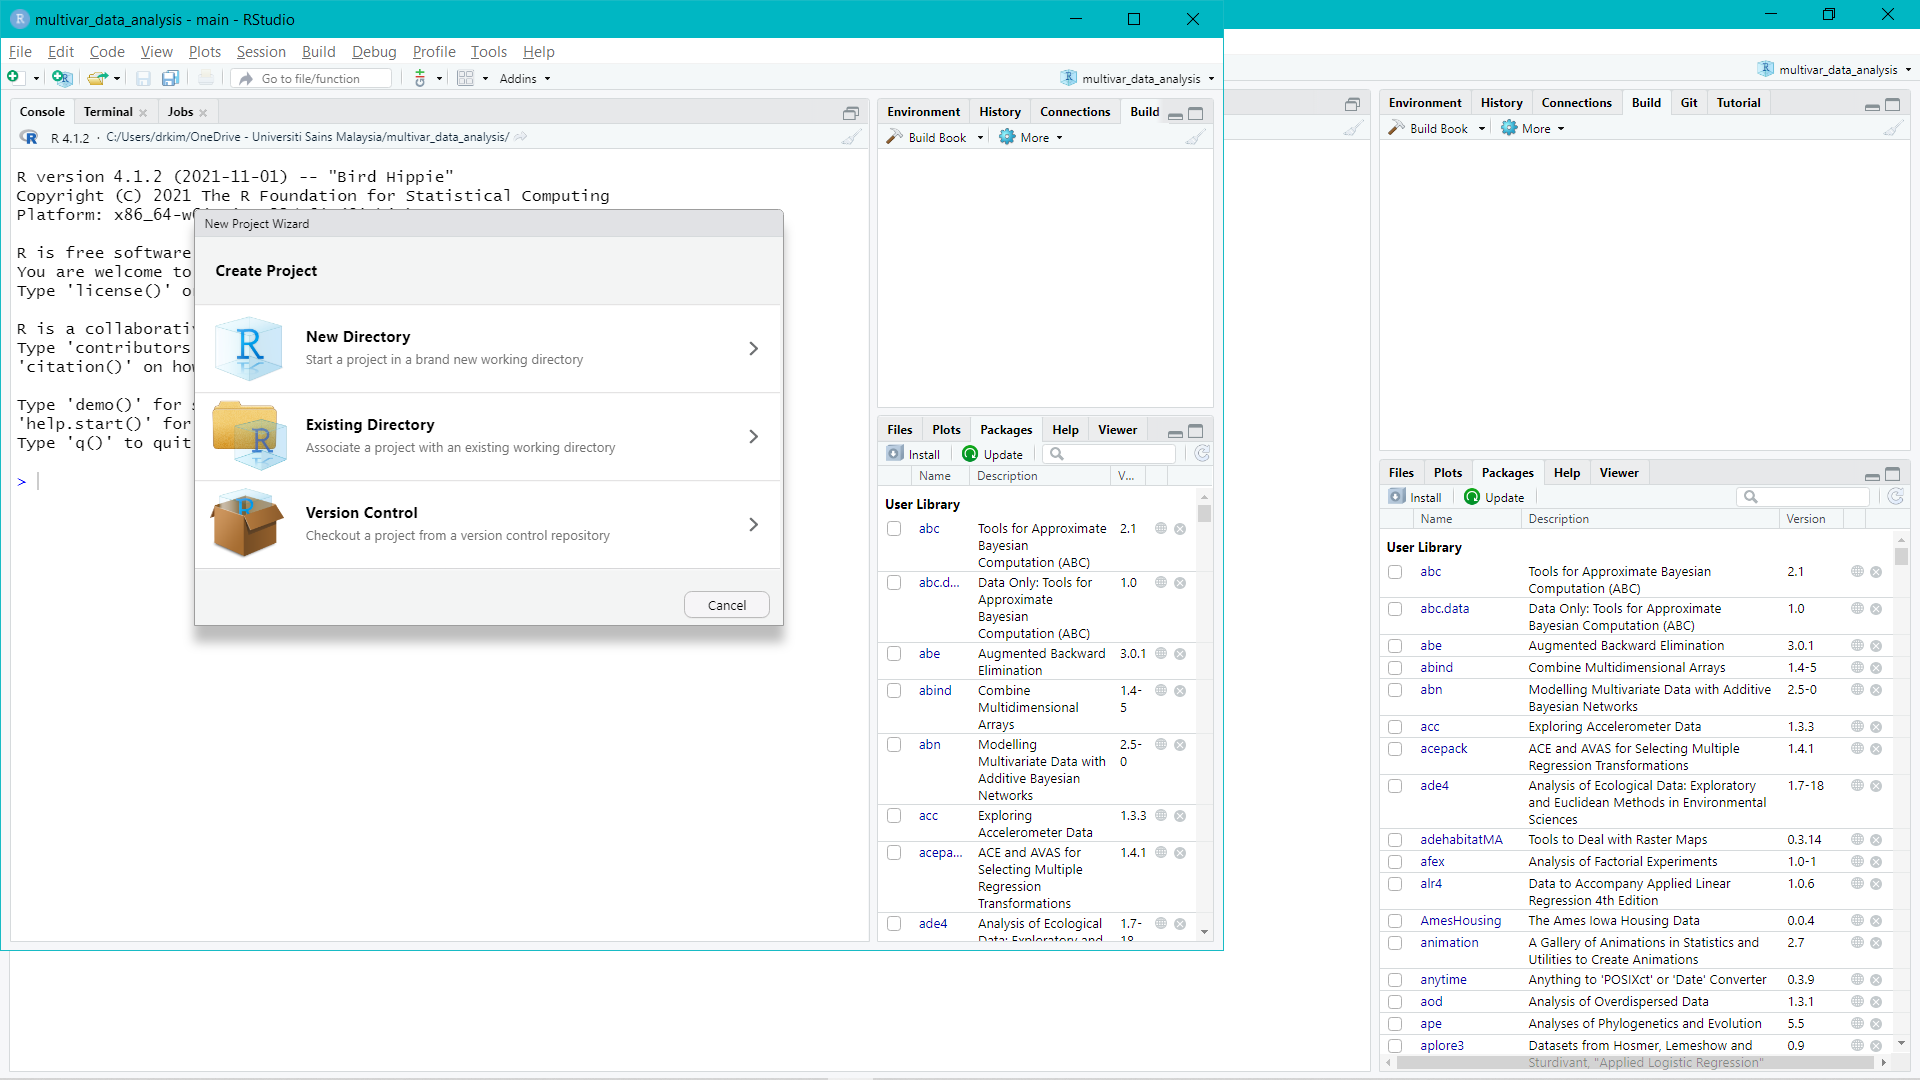
\includegraphics{13newproject.png}
\caption{New Project and Version Control}
\end{figure}

and then click \texttt{Git}

\begin{figure}
\centering
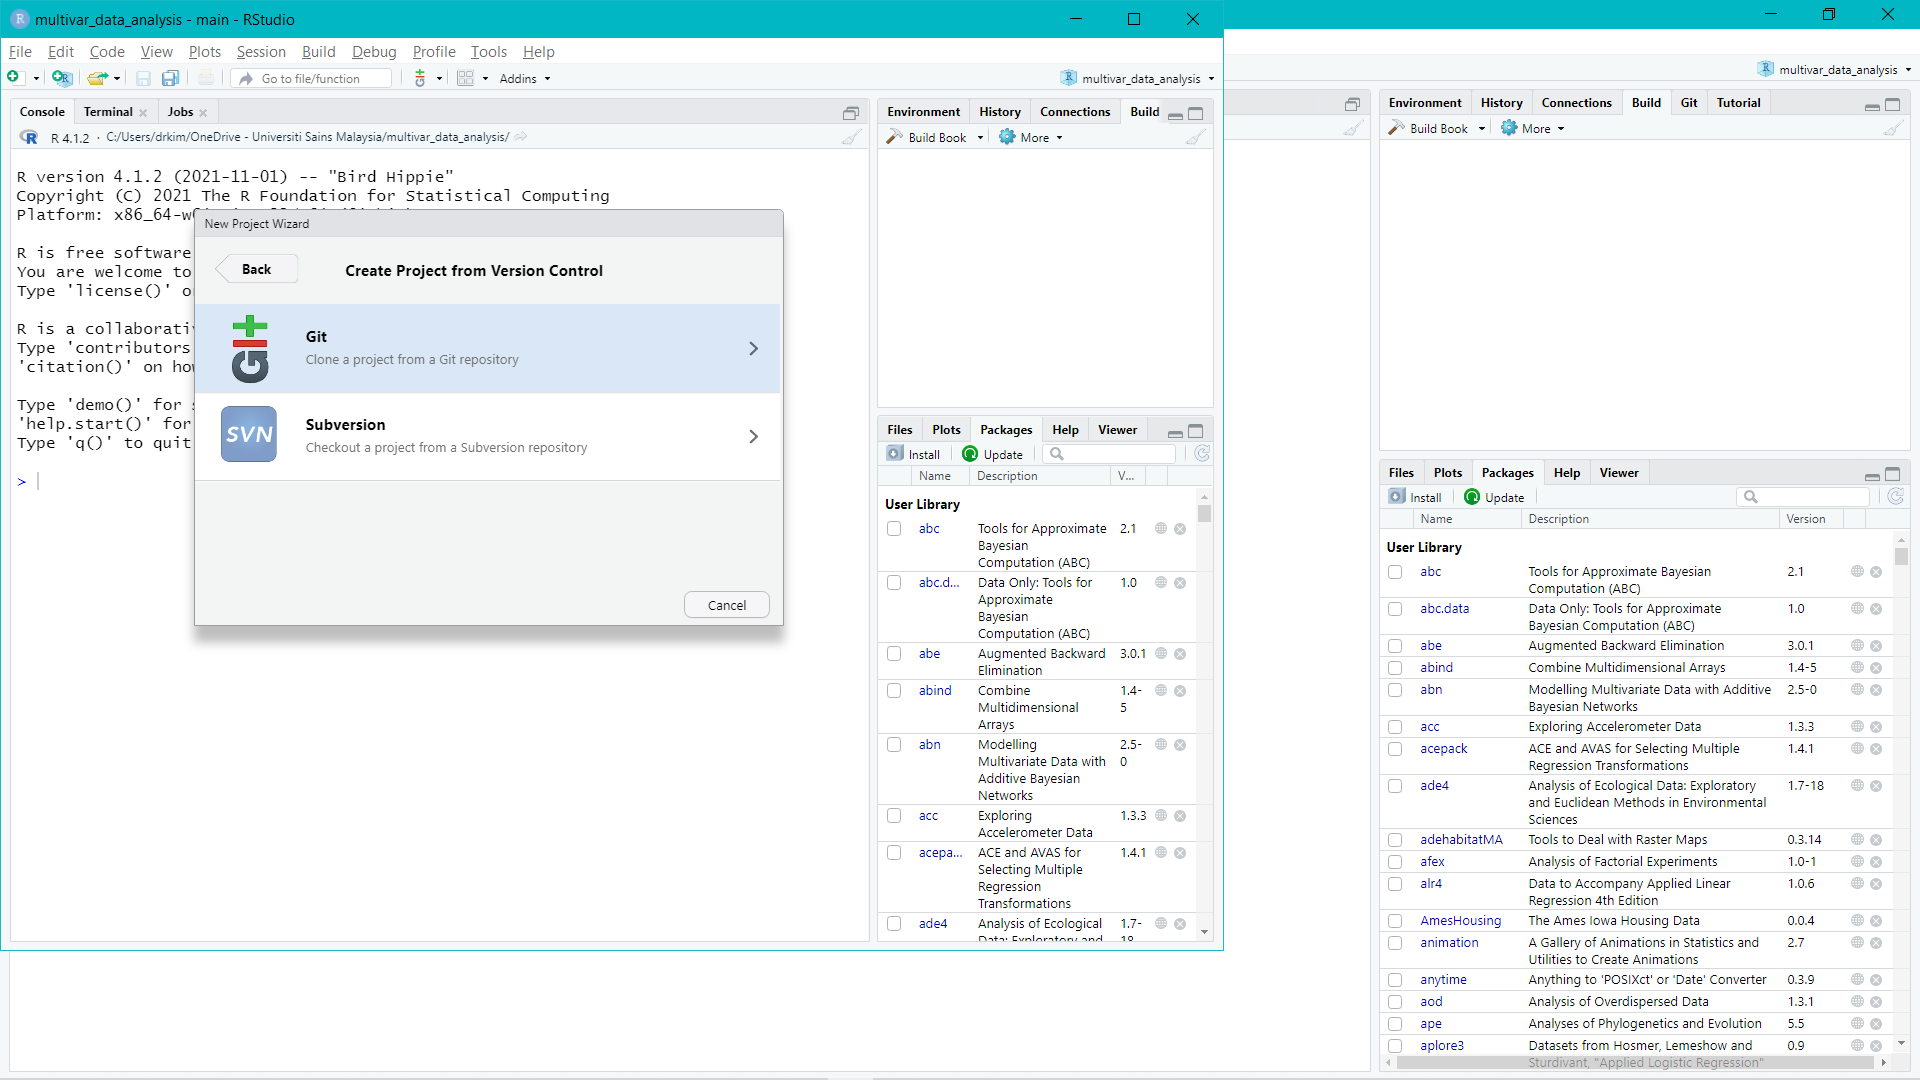
\includegraphics{14git.png}
\caption{Git}
\end{figure}

And remember the HTTPS that we have copied from our \texttt{dataset-for-RMed} GitHub\index{GitHub} repository

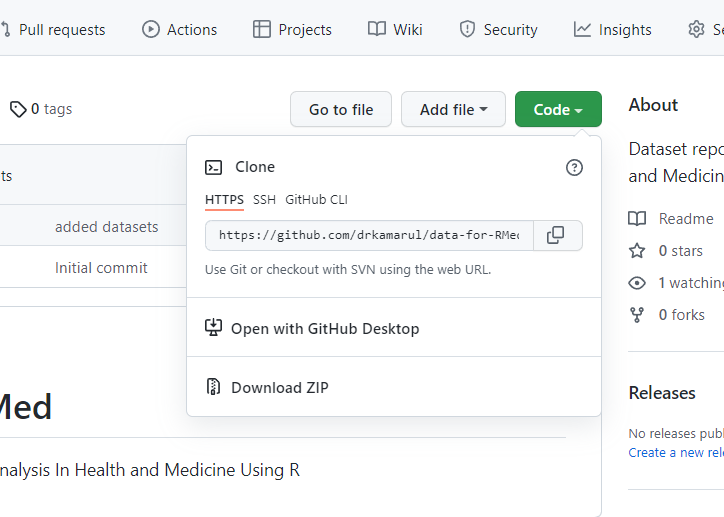
\includegraphics{15copyurlgit.png}
Now,

\begin{itemize}
\tightlist
\item
  paste the HTTPS link
\item
  the Project directory name will be automatically filled
\item
  Click on \texttt{Browse}, and you may choose whichever folder that you prefer. We recommend you to use home directory (such as \texttt{Documents})
\end{itemize}

\begin{figure}
\centering
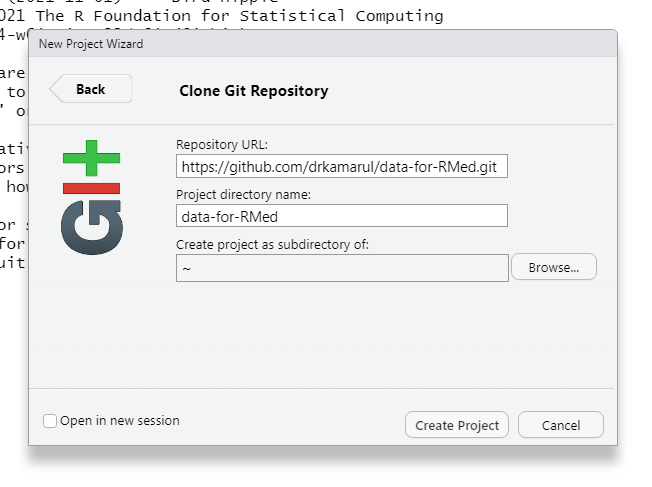
\includegraphics{16clonegit.png}
\caption{Clone Git Repository}
\end{figure}

And now RStudio will create a new working directory\index{Working directory} on your local machine. This working directory contains the same folder and file structures with the GitHub repository\index{GitHub repository}

\begin{figure}
\centering
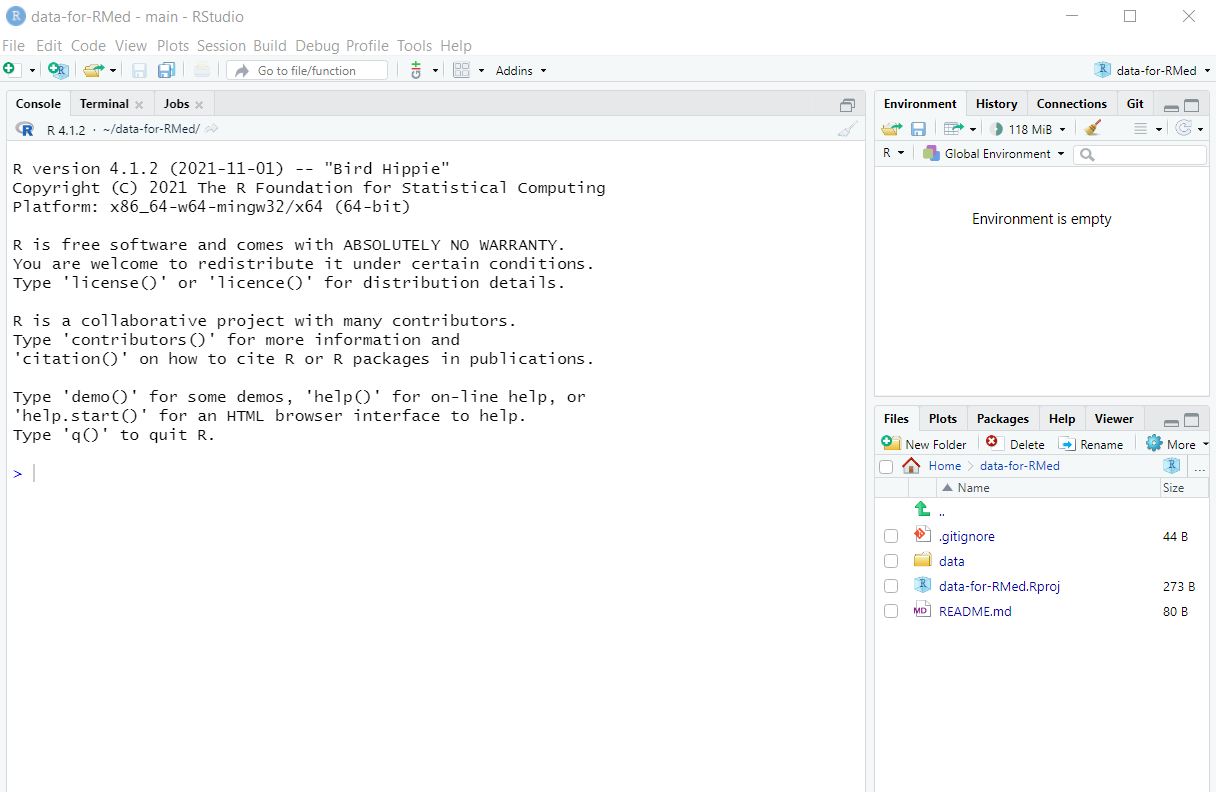
\includegraphics{17rstudio.png}
\caption{RStudio Project}
\end{figure}

\hypertarget{data-visualization}{%
\chapter{Data Visualization}\label{data-visualization}}

\hypertarget{introduction-1}{%
\section{Introduction}\label{introduction-1}}

Data visualization is viewed by many disciplines as a modern equivalent of visual communication. It involves the creation and study of the visual representation of data. Data visualization requires ``information that has been abstracted in some schematic form, including attributes or variables for the units of information''. You can read more about data visualization here \url{https://en.m.wikipedia.org/wiki/Data_visualization} and here \url{https://en.m.wikipedia.org/wiki/Michael_Friendly}

In this chapter, we want to achieve these objectives:

\begin{enumerate}
\def\labelenumi{\arabic{enumi}.}
\tightlist
\item
  To introduce concept of data visualization
\item
  To describe ingredients for good graphics
\item
  To generate plots using \textbf{ggplot} packages
\item
  To save plots in different format and settings
\end{enumerate}

\hypertarget{history-and-objectives-of-data-visualization}{%
\section{History and objectives of Data Visualization}\label{history-and-objectives-of-data-visualization}}

In his 1983 book which carried the title \emph{The Visual Display of Quantitative Information}, the author Edward Tufte defines \textbf{graphical displays} and principles for effective graphical display. The book mentioned that ``Excellence in statistical graphics consists of complex ideas communicated with clarity, precision and efficiency.''

Visualization is the process of representing data graphically and interacting with these representations. The objective is to gain insight into the data. Some of the processes are outlined here \url{http://researcher.watson.ibm.com/researcher/view_group.php?id=143}

\hypertarget{ingredients-for-good-graphics}{%
\section{Ingredients for Good Graphics}\label{ingredients-for-good-graphics}}

We require these features to make good graphics:

\begin{enumerate}
\def\labelenumi{\arabic{enumi}.}
\tightlist
\item
  Good data
\item
  Priorities on substance rather than methodology, graphic design, the technology of graphic production or something else
\item
  No distortion to what the data has to say
\item
  Presence of many numbers in a small space
\item
  Coherence for large data sets
\item
  They encourage the eye to compare different pieces of data
\item
  They reveal data at several levels of detail, from a broad overview to the fine structure
\item
  Serve a reasonably clear purpose: description, exploration, tabulation or decoration
\item
  Be closely integrated with the statistical and verbal descriptions of a data set.
\end{enumerate}

\hypertarget{graphics-packages-in-r}{%
\section{Graphics Packages in R}\label{graphics-packages-in-r}}

There are many \textbf{graphics packages} in R. Some packages perform general data visualization or graphical taskss. The others provide specific graphics for certain statistical or data analyses.

The popular general purpose graphics packages in R are:

\begin{enumerate}
\def\labelenumi{\arabic{enumi}.}
\tightlist
\item
  \textbf{graphics}\index{graphics} : a base R package, which means it is loaded everytime we open R
\item
  \textbf{ggplot2}\index{ggplot2} : a user-contributed package by RStudio
\item
  \textbf{lattice}\index{lattice} : a user-contributed package
\end{enumerate}

Except for \textbf{graphics}\index{graphics} package (a base R package), other packages need to downloaded and installed into your R library. A few examples more specific graphical packages include:

\begin{enumerate}
\def\labelenumi{\arabic{enumi}.}
\tightlist
\item
  \textbf{survminer::ggsurvlot} : The \textbf{survminer}\index{survminer} R package provides functions for facilitating survival analysis and visualization.
\item
  \textbf{sjPlot}\index{sjPlot} : Collection of plotting and table output functions for data visualization
\end{enumerate}

\hypertarget{the-ggplot2-package}{%
\section{\texorpdfstring{The \textbf{ggplot2}\index{ggplot2} Package}{The ggplot2 Package}}\label{the-ggplot2-package}}

For this book, we will focus on using the \textbf{ggplot2}\index{ggplot2} package. The \textbf{ggplot2}\index{ggplot2} package is an elegant, easy and versatile general graphics package in R. It implements the \textbf{grammar of graphics}\index{Grammar of graphics} concept. The advantage of this concept is that, it fasten the process of learning graphics. It also facilitates the process of creating complex graphics

To work with \textbf{ggplot2}\index{ggplot2}, remember to

\begin{itemize}
\tightlist
\item
  start R codes with \texttt{ggplot()}
\item
  identify which data to plot: \texttt{data\ =\ Your\ Data}
\item
  state variables to plot: \texttt{aes(x\ =\ Variable\ on\ x-axis,\ y\ =\ Variable\ on\ y-axis\ )}
\item
  choose type of graph: for example \texttt{geom\_histogram()} for histogram, and \texttt{geom\_points()} for scatterplots\index{Scatterplot}
\end{itemize}

The official website for ggplot2\index{ggplot2} is here \url{https://ggplot2.tidyverse.org/}. It has excellent resources. It states that:

\emph{ggplot2\index{ggplot2} is a plotting system for R, based on the grammar of graphics\index{Grammar of graphics}, which tries to take the good parts of base and lattice\index{lattice} graphics and none of the bad parts. It takes care of many of the fiddly details that make plotting a hassle (like drawing legends) as well as providing a powerful model of graphics that makes it easy to produce complex multi-layered graphics.}

\hypertarget{preparation}{%
\section{Preparation}\label{preparation}}

\hypertarget{create-a-new-rstudio-project}{%
\subsection{Create a New RStudio Project}\label{create-a-new-rstudio-project}}

It is always recommended that to start working on data analysis in RStudio, you create first a new project.

Go to File, then click New Project.

You can create a new R project based on existing directory. This method is useful because an RStudio project keep your data, your analysis, and outputs in a clean dedicated folder or sets of folders.If you do not want to create a new project, then make sure you are inside the correct directory (the working directory). The working directory is a folder where you store.

Type \texttt{getwd()} in your Console to display your working directory. Inside your working directory, you should see and keep

\begin{enumerate}
\def\labelenumi{\arabic{enumi}.}
\tightlist
\item
  dataset or datasets
\item
  outputs - plots
\item
  codes (R scripts \texttt{.R}, R markdown files \texttt{.Rmd}\index{R markdown})
\end{enumerate}

\hypertarget{important-questions-when-making-graphs}{%
\subsection{Important Questions when Making Graphs}\label{important-questions-when-making-graphs}}

You must ask yourselves these:

\begin{enumerate}
\def\labelenumi{\arabic{enumi}.}
\tightlist
\item
  Which variable or variables do I want to plot?
\item
  What is (or are) the type of that variable?
\end{enumerate}

\begin{itemize}
\tightlist
\item
  Are they factor (categorical) variables ?
\item
  Are they numerical variables?
\end{itemize}

\begin{enumerate}
\def\labelenumi{\arabic{enumi}.}
\setcounter{enumi}{2}
\tightlist
\item
  Am I going to plot
\end{enumerate}

\begin{itemize}
\tightlist
\item
  a single variable?
\item
  two variables together?
\item
  three variables together?
\end{itemize}

\hypertarget{read-data}{%
\subsection{Read Data}\label{read-data}}

The common data formats include

\begin{enumerate}
\def\labelenumi{\arabic{enumi}.}
\tightlist
\item
  comma separated files (\texttt{.csv})
\item
  MS Excel file (\texttt{.xlsx})
\item
  SPSS\index{SPSS} file (\texttt{.sav})
\item
  Stata\index{STATA} file (\texttt{.dta})
\item
  SAS\index{SAS} file
\end{enumerate}

Packages that read these data include \textbf{haven}\index{haven} and \textbf{rio}\index{rio} packages. Below are the functions to read SAS\index{SAS}, SPSS\index{SPSS} and Stata\index{STATA} file using the \textbf{haven}\index{haven} package.

\begin{enumerate}
\def\labelenumi{\arabic{enumi}.}
\tightlist
\item
  SAS\index{SAS}: \texttt{read\_sas()} reads .sas7bdat + .sas7bcat files and read\_xpt() reads SAS\index{SAS} transport files (version 5 and version 8). write\_sas() writes .sas7bdat files.
\item
  SPSS\index{SPSS}: \texttt{read\_sav()} reads .sav files and read\_por() reads the older .por files. write\_sav() writes .sav files.
\item
  Stata\index{STATA}: \texttt{read\_dta()} reads .dta files (up to version 15). write\_dta() writes .dta files (versions 8-15).
\end{enumerate}

Sometime, we may want to import data from databases. For beginners, this experience is less common. However, the skill to import data from databases are getting more important and more common. Fortunately, R can easily import and read these data. Some examples of common databases format are:

\begin{enumerate}
\def\labelenumi{\arabic{enumi}.}
\tightlist
\item
  MySQL
\item
  SQLite
\item
  Postgresql
\item
  Mariadb
\end{enumerate}

\hypertarget{load-the-library}{%
\subsection{Load the Library}\label{load-the-library}}

The \textbf{ggplot2}\index{ggplot2} package is one of the core member of \textbf{tidyverse}\index{tidyverse} metapackage (\url{https://www.tidyverse.org/}). So, if we load the \textbf{tidyverse}\index{tidyverse} package, it means we are also loading other packages under the \textbf{tidyverse}\index{tidyverse} metapackage: which include \textbf{dplyr}\index{dplyr}, \textbf{readr}\index{readr}, \textbf{ggplot2}\index{ggplot2}.

Loading a package will give you access to

\begin{enumerate}
\def\labelenumi{\arabic{enumi}.}
\tightlist
\item
  help pages of the package
\item
  functions available in the package
\item
  sample datasets (not all packages contain this feature)
\end{enumerate}

We will also load the \textbf{here}\index{here} package. This is useful to point to the codes to a specific folder in the project space. We will see this in action later.

\begin{Shaded}
\begin{Highlighting}[]
\FunctionTok{library}\NormalTok{(tidyverse)}
\end{Highlighting}
\end{Shaded}

\begin{verbatim}
## -- Attaching packages --------------------------------------- tidyverse 1.3.2 --
## v ggplot2 3.3.6     v purrr   0.3.4
## v tibble  3.1.8     v dplyr   1.0.9
## v tidyr   1.2.0     v stringr 1.4.0
## v readr   2.1.2     v forcats 0.5.1
## -- Conflicts ------------------------------------------ tidyverse_conflicts() --
## x dplyr::filter() masks stats::filter()
## x dplyr::lag()    masks stats::lag()
\end{verbatim}

\begin{Shaded}
\begin{Highlighting}[]
\FunctionTok{library}\NormalTok{(here)}
\end{Highlighting}
\end{Shaded}

\begin{verbatim}
## here() starts at /home/wnarifin/Clouds/pCloud_Local/multivar_data_analysis
\end{verbatim}

If you run the code and you get this message \emph{there is no package called tidyverse}\index{tidyverse}, you need to install the \textbf{tidyverse}\index{tidyverse} package on your R IDE.

To install the package, type \texttt{install.package("tidyverse")}\index{tidyverse} in the Console. Once the installation is complete, type \texttt{library(tidyverse)}\index{tidyverse} to load the package.

Alternatively, you can use the GUI\index{GUI} to install the package:

\begin{figure}
\centering
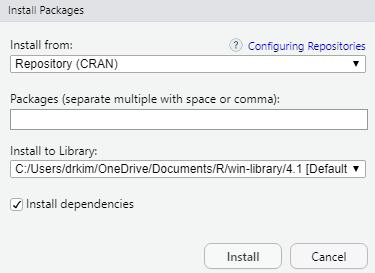
\includegraphics{tidyverse.png}
\caption{Packages pane}
\end{figure}

Now, type the package you want to install. For example you want to install the \textbf{tidyverse}\index{tidyverse} package

\begin{figure}
\centering
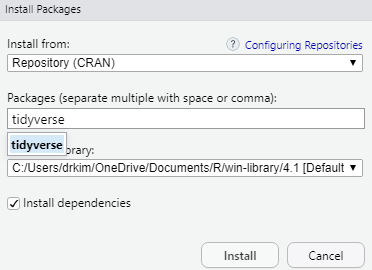
\includegraphics{tidyverse2.png}
\caption{Typing the package to install}
\end{figure}

\hypertarget{read-dataset}{%
\subsection{Read Dataset}\label{read-dataset}}

For now, we will use two datasets:

\begin{enumerate}
\def\labelenumi{\alph{enumi}.}
\tightlist
\item
  the built-in dataset in the \textbf{gapminder}\index{gapminder} package. You can read more about \emph{gapminder}\index{gapminder} from \url{https://www.gapminder.org/}. The gapminder\index{gapminder} website contains many useful datasets and show wonderful graphics. It is made popular by Dr Hans Rosling.
\item
  the dataset of patients admitted with peptic ulcer disease \texttt{peptic\_ulcer.xlsx}. It is in the MS Excel format.
\end{enumerate}

To load the \textbf{gapminder}\index{gapminder} package, type

\begin{Shaded}
\begin{Highlighting}[]
\FunctionTok{library}\NormalTok{(gapminder)}
\end{Highlighting}
\end{Shaded}

call the data \emph{gapminder} into R and browse the first 6 observations of the \emph{gapminder} data. The codes below shows

\begin{itemize}
\tightlist
\item
  assigning gapminder as a dataset
\item
  a pipe that connects two codes (\texttt{gapminder} and \texttt{slice})
\item
  a function called \texttt{slice()} that select rows of the dataset
\end{itemize}

\begin{Shaded}
\begin{Highlighting}[]
\NormalTok{gapminder }\OtherTok{\textless{}{-}}\NormalTok{ gapminder}
\NormalTok{gapminder }\SpecialCharTok{\%\textgreater{}\%} 
  \FunctionTok{slice}\NormalTok{(}\DecValTok{1}\SpecialCharTok{:}\DecValTok{4}\NormalTok{)}
\end{Highlighting}
\end{Shaded}

\begin{verbatim}
## # A tibble: 4 x 6
##   country     continent  year lifeExp      pop gdpPercap
##   <fct>       <fct>     <int>   <dbl>    <int>     <dbl>
## 1 Afghanistan Asia       1952    28.8  8425333      779.
## 2 Afghanistan Asia       1957    30.3  9240934      821.
## 3 Afghanistan Asia       1962    32.0 10267083      853.
## 4 Afghanistan Asia       1967    34.0 11537966      836.
\end{verbatim}

We can list the variables and look at the type of the variables in the gapminder dataset

\begin{Shaded}
\begin{Highlighting}[]
\FunctionTok{glimpse}\NormalTok{(gapminder)}
\end{Highlighting}
\end{Shaded}

\begin{verbatim}
## Rows: 1,704
## Columns: 6
## $ country   <fct> "Afghanistan", "Afghanistan", "Afghanistan", "Afghanistan", ~
## $ continent <fct> Asia, Asia, Asia, Asia, Asia, Asia, Asia, Asia, Asia, Asia, ~
## $ year      <int> 1952, 1957, 1962, 1967, 1972, 1977, 1982, 1987, 1992, 1997, ~
## $ lifeExp   <dbl> 28.801, 30.332, 31.997, 34.020, 36.088, 38.438, 39.854, 40.8~
## $ pop       <int> 8425333, 9240934, 10267083, 11537966, 13079460, 14880372, 12~
## $ gdpPercap <dbl> 779.4453, 820.8530, 853.1007, 836.1971, 739.9811, 786.1134, ~
\end{verbatim}

The \emph{gapminder} data have

\begin{enumerate}
\def\labelenumi{\arabic{enumi}.}
\tightlist
\item
  Six (6) variables
\item
  A total of 1704 observations
\item
  Two factor variables, 2 integer variables and 2 numeric (\texttt{dbl}) variables
\end{enumerate}

We can examine the basic statistics of the gapminder datasets by using \texttt{summary()}. This function will list

\begin{enumerate}
\def\labelenumi{\arabic{enumi}.}
\tightlist
\item
  the frequencies
\item
  some descriptive statistics: min, 1st quartile, median, mean, 3rd quartile and max
\end{enumerate}

\begin{Shaded}
\begin{Highlighting}[]
\FunctionTok{summary}\NormalTok{(gapminder)}
\end{Highlighting}
\end{Shaded}

\begin{verbatim}
##         country        continent        year         lifeExp     
##  Afghanistan:  12   Africa  :624   Min.   :1952   Min.   :23.60  
##  Albania    :  12   Americas:300   1st Qu.:1966   1st Qu.:48.20  
##  Algeria    :  12   Asia    :396   Median :1980   Median :60.71  
##  Angola     :  12   Europe  :360   Mean   :1980   Mean   :59.47  
##  Argentina  :  12   Oceania : 24   3rd Qu.:1993   3rd Qu.:70.85  
##  Australia  :  12                  Max.   :2007   Max.   :82.60  
##  (Other)    :1632                                                
##       pop              gdpPercap       
##  Min.   :6.001e+04   Min.   :   241.2  
##  1st Qu.:2.794e+06   1st Qu.:  1202.1  
##  Median :7.024e+06   Median :  3531.8  
##  Mean   :2.960e+07   Mean   :  7215.3  
##  3rd Qu.:1.959e+07   3rd Qu.:  9325.5  
##  Max.   :1.319e+09   Max.   :113523.1  
## 
\end{verbatim}

To know more about the package, we can use the \(?\) mark

\begin{Shaded}
\begin{Highlighting}[]
\NormalTok{?gapminder}
\end{Highlighting}
\end{Shaded}

\hypertarget{basic-plots}{%
\section{\texorpdfstring{Basic Plots\index{Basic plots}}{Basic Plots}}\label{basic-plots}}

Let us start by creating a simple plot using these arguments:

\begin{itemize}
\tightlist
\item
  data : \texttt{data\ =\ gapminder}
\item
  variables : \texttt{x\ =\ year}, \texttt{y\ =\ \ lifeExp}
\item
  graph scatterplot\index{Scatterplot} : \texttt{geom\_point()}
\end{itemize}

In \textbf{ggplot2}\index{ggplot2} which is a package under \textbf{tidyverse}\index{tidyverse} package, we may use the \(+\) sign to connect the function. And in R, your codes can span multiple lines. This will increase the visibility of the codes.

\begin{Shaded}
\begin{Highlighting}[]
\FunctionTok{ggplot}\NormalTok{(}\AttributeTok{data =}\NormalTok{ gapminder) }\SpecialCharTok{+}
  \FunctionTok{geom\_point}\NormalTok{(}\AttributeTok{mapping =} \FunctionTok{aes}\NormalTok{(}\AttributeTok{x =}\NormalTok{ year, }\AttributeTok{y =}\NormalTok{ lifeExp))}
\end{Highlighting}
\end{Shaded}

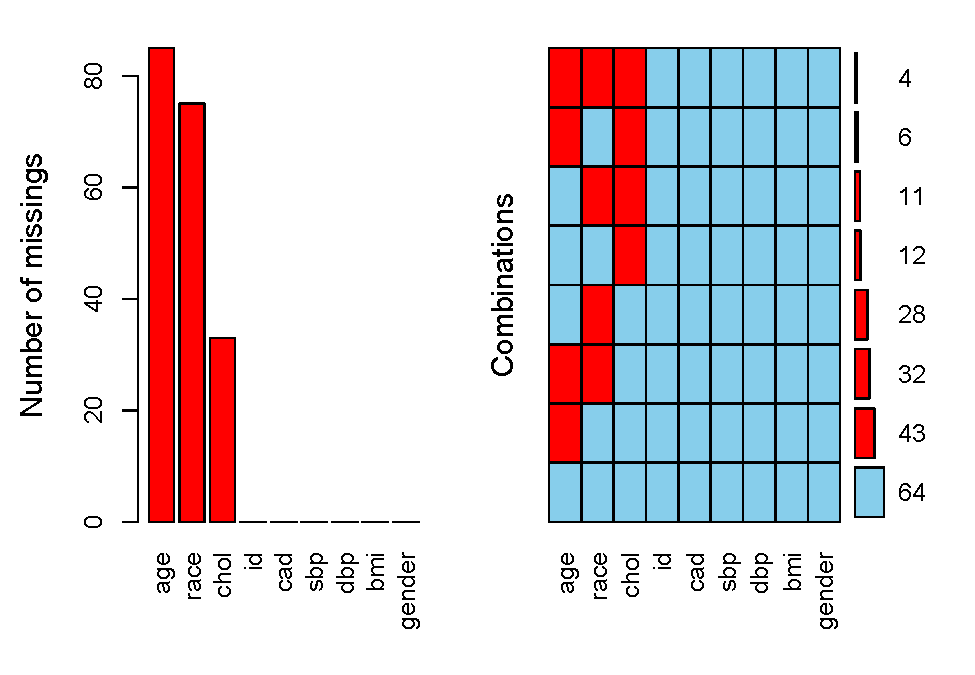
\includegraphics{03_data_visualization_files/figure-latex/unnamed-chunk-7-1.pdf}

Now, we can see

\begin{enumerate}
\def\labelenumi{\arabic{enumi}.}
\tightlist
\item
  a scatterplot\index{Scatterplot}
\item
  the scatterplot\index{Scatterplot} shows the relationship between year and life expectancy.
\item
  as variable year advances, the life expectancy increases.
\end{enumerate}

What do the codes tell us?

\begin{itemize}
\tightlist
\item
  the \texttt{ggplot()} tells R to be ready to make plot from a specified data.
\item
  And \texttt{geom\_point()} tells R to make a scatter plot.
\end{itemize}

More resources about \textbf{ggplot2}\index{ggplot2} package is available here \url{https://ggplot2.tidyverse.org/reference/ggplot.html}

\hypertarget{adding-another-variable}{%
\section{Adding another variable}\label{adding-another-variable}}

We can see that the variables we want to plot are specified by \texttt{aes()}. We can add a third variable to make a more complex plot. For example:

\begin{enumerate}
\def\labelenumi{\arabic{enumi}.}
\tightlist
\item
  data : \texttt{data\ =\ gapminder}
\item
  variables : \texttt{x\ =\ year}, \texttt{y\ =\ lifeExp}, \texttt{colour\ =\ continent}
\end{enumerate}

For this, the objective to create plot might be to see the relationship between year and life expectancy based on continent.

\begin{Shaded}
\begin{Highlighting}[]
\FunctionTok{ggplot}\NormalTok{(}\AttributeTok{data =}\NormalTok{ gapminder) }\SpecialCharTok{+}
  \FunctionTok{geom\_point}\NormalTok{(}\AttributeTok{mapping =} \FunctionTok{aes}\NormalTok{(}\AttributeTok{x =}\NormalTok{ year, }
                           \AttributeTok{y =}\NormalTok{ lifeExp, }
                           \AttributeTok{colour =}\NormalTok{ continent))}
\end{Highlighting}
\end{Shaded}

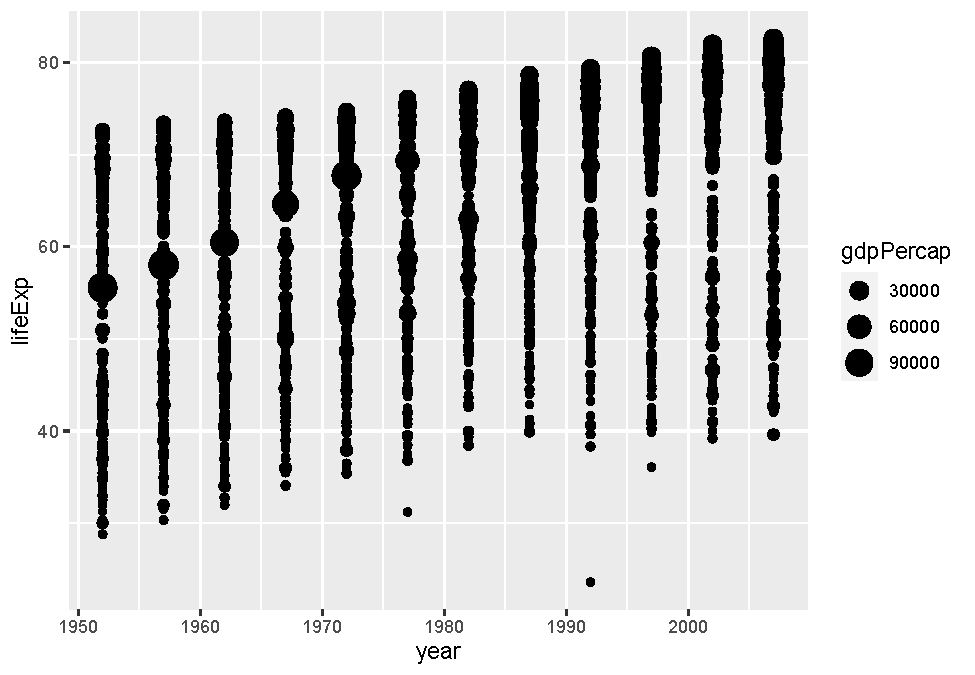
\includegraphics{03_data_visualization_files/figure-latex/unnamed-chunk-8-1.pdf}

What can you see from the scatterplot\index{Scatterplot}? You may notice that

\begin{enumerate}
\def\labelenumi{\arabic{enumi}.}
\tightlist
\item
  Europe countries have high life expectancy
\item
  Africa countries have lower life expectancy
\item
  One Asia country looks like an outlier (very low life expectancy)
\item
  One Africa country looks like an outlier (very low life expectancy)
\end{enumerate}

Now, we will replace the third variable with Gross Domestic Product (gdpPercap) and make the plot correlates with the size of gdpPerCap

\begin{Shaded}
\begin{Highlighting}[]
\FunctionTok{ggplot}\NormalTok{(}\AttributeTok{data =}\NormalTok{ gapminder) }\SpecialCharTok{+}
  \FunctionTok{geom\_point}\NormalTok{(}\AttributeTok{mapping =} \FunctionTok{aes}\NormalTok{(}\AttributeTok{x =}\NormalTok{ year, }
                           \AttributeTok{y =}\NormalTok{ lifeExp, }
                           \AttributeTok{size =}\NormalTok{ gdpPercap))}
\end{Highlighting}
\end{Shaded}

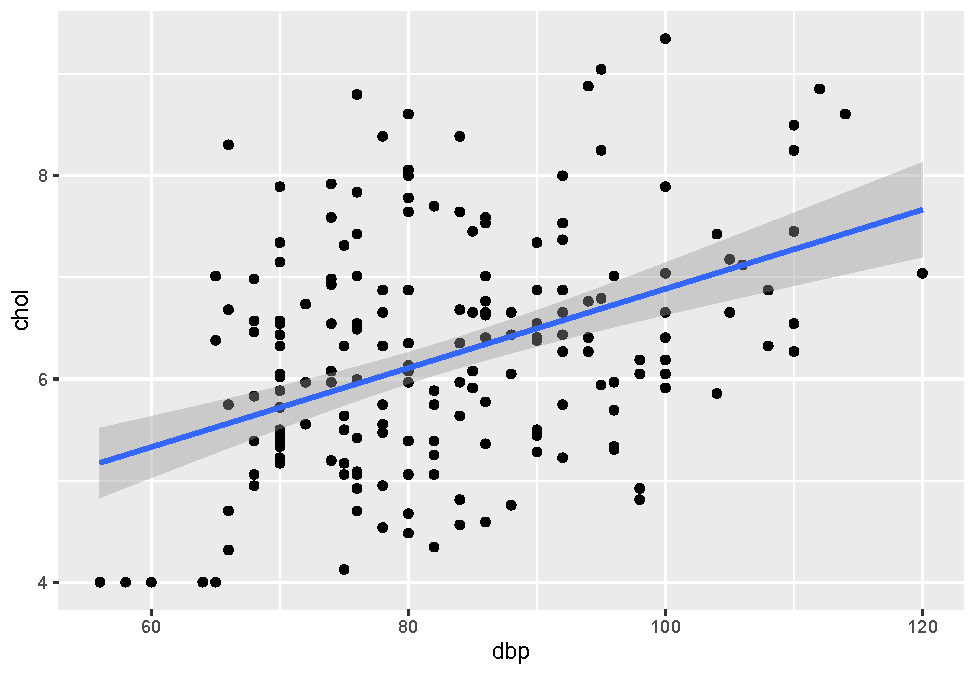
\includegraphics{03_data_visualization_files/figure-latex/unnamed-chunk-9-1.pdf}

\emph{ggplot2}\index{ggplot2} will automatically assign a unique level of the aesthetic (here a unique color) to each unique value of the variable, a process known as scaling. \emph{ggplot2}\index{ggplot2} will also add a legend that explains which levels correspond to which values. The plot suggests that with higher gdpPerCap, there is also longer lifeExp.

Instead of using colour, we can use different shapes. This is useful especially in the instances where there is no facility to print out colourful plots.

\begin{Shaded}
\begin{Highlighting}[]
\FunctionTok{ggplot}\NormalTok{(}\AttributeTok{data =}\NormalTok{ gapminder) }\SpecialCharTok{+}
  \FunctionTok{geom\_point}\NormalTok{(}\AttributeTok{mapping =} \FunctionTok{aes}\NormalTok{(}\AttributeTok{x =}\NormalTok{ year, }
                           \AttributeTok{y =}\NormalTok{ lifeExp, }
                           \AttributeTok{shape =}\NormalTok{ continent))}
\end{Highlighting}
\end{Shaded}

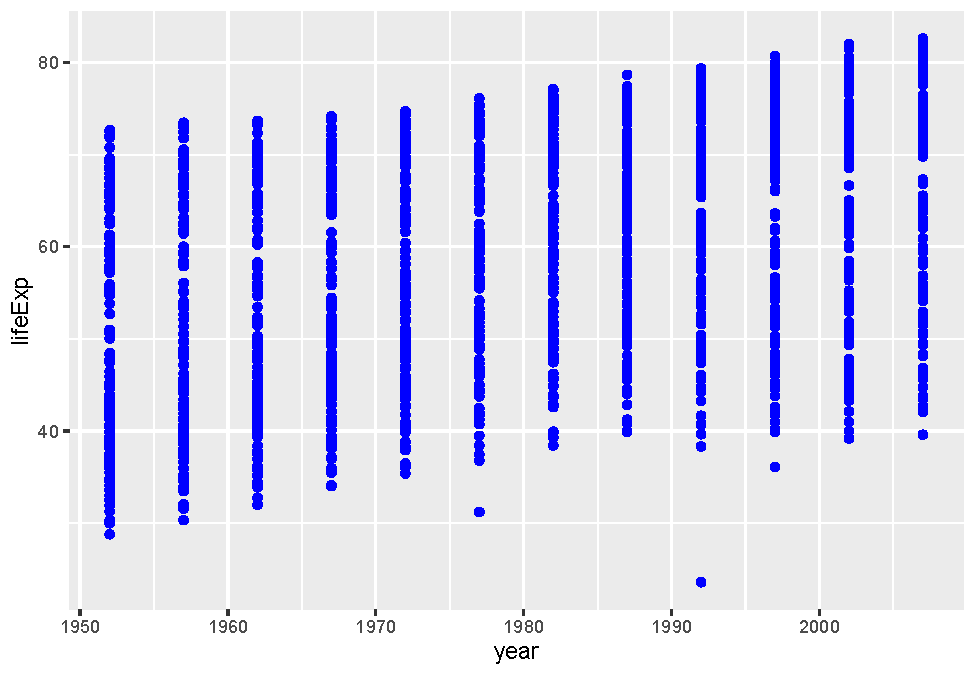
\includegraphics{03_data_visualization_files/figure-latex/unnamed-chunk-10-1.pdf}

But, see what will happen if we set the colour and shape like below but outside the \texttt{aes} parentheses. For example, let set the parameter colour to \texttt{blue}

\begin{Shaded}
\begin{Highlighting}[]
\FunctionTok{ggplot}\NormalTok{(}\AttributeTok{data =}\NormalTok{ gapminder) }\SpecialCharTok{+}
  \FunctionTok{geom\_point}\NormalTok{(}\AttributeTok{mapping =} \FunctionTok{aes}\NormalTok{(}\AttributeTok{x =}\NormalTok{ year, }\AttributeTok{y =}\NormalTok{ lifeExp), }
             \AttributeTok{colour =} \StringTok{\textquotesingle{}blue\textquotesingle{}}\NormalTok{)}
\end{Highlighting}
\end{Shaded}

\includegraphics{03_data_visualization_files/figure-latex/unnamed-chunk-11-1.pdf}

And then parameter shape to plus (which is represented by number 3).

\begin{Shaded}
\begin{Highlighting}[]
\FunctionTok{ggplot}\NormalTok{(}\AttributeTok{data =}\NormalTok{ gapminder) }\SpecialCharTok{+}
  \FunctionTok{geom\_point}\NormalTok{(}\AttributeTok{mapping =} \FunctionTok{aes}\NormalTok{(}\AttributeTok{x =}\NormalTok{ year, }\AttributeTok{y =}\NormalTok{ lifeExp), }
             \AttributeTok{shape =} \DecValTok{3}\NormalTok{)}
\end{Highlighting}
\end{Shaded}

\includegraphics{03_data_visualization_files/figure-latex/unnamed-chunk-12-1.pdf}

We may wonder what number corresponds to what type of shape. We can type \texttt{?pch}. And we will see in the Viewer pane, the explanation about the shape available in R. It also shows what number that corresponds to what shape.

\hypertarget{making-subplots}{%
\section{Making Subplots}\label{making-subplots}}

We can split our plots based on a factor variable and make subplots using the \texttt{facet()}. For example, if we want to make subplots based on continents, then we need to set these parameters:

\begin{itemize}
\tightlist
\item
  data = gapminder
\item
  variable \texttt{year} on the x-axis and \texttt{lifeExp} on the y-axis
\item
  split the plot based on continent
\item
  set the number of rows for the plot at 3
\end{itemize}

\begin{Shaded}
\begin{Highlighting}[]
\FunctionTok{ggplot}\NormalTok{(}\AttributeTok{data =}\NormalTok{ gapminder) }\SpecialCharTok{+}
  \FunctionTok{geom\_point}\NormalTok{(}\AttributeTok{mapping =} \FunctionTok{aes}\NormalTok{(}\AttributeTok{x =}\NormalTok{ year, }\AttributeTok{y =}\NormalTok{ lifeExp)) }\SpecialCharTok{+} 
  \FunctionTok{facet\_wrap}\NormalTok{(}\SpecialCharTok{\textasciitilde{}}\NormalTok{ continent, }\AttributeTok{nrow =} \DecValTok{3}\NormalTok{)}
\end{Highlighting}
\end{Shaded}

\includegraphics{03_data_visualization_files/figure-latex/unnamed-chunk-13-1.pdf}

Now, what happen if we change the value for the \texttt{nrow}

\begin{Shaded}
\begin{Highlighting}[]
\FunctionTok{ggplot}\NormalTok{(}\AttributeTok{data =}\NormalTok{ gapminder) }\SpecialCharTok{+}
  \FunctionTok{geom\_point}\NormalTok{(}\AttributeTok{mapping =} \FunctionTok{aes}\NormalTok{(}\AttributeTok{x =}\NormalTok{ year, }\AttributeTok{y =}\NormalTok{ lifeExp)) }\SpecialCharTok{+} 
  \FunctionTok{facet\_wrap}\NormalTok{(}\SpecialCharTok{\textasciitilde{}}\NormalTok{ continent, }\AttributeTok{nrow =} \DecValTok{2}\NormalTok{)}
\end{Highlighting}
\end{Shaded}

\includegraphics{03_data_visualization_files/figure-latex/unnamed-chunk-14-1.pdf}

\hypertarget{overlaying-plots}{%
\section{Overlaying Plots}\label{overlaying-plots}}

Each \texttt{geom\_X()} in ggplot2\index{ggplot2} indicates different visual objects.

This is a scatterplot\index{Scatterplot}

\begin{Shaded}
\begin{Highlighting}[]
\FunctionTok{ggplot}\NormalTok{(}\AttributeTok{data =}\NormalTok{ gapminder) }\SpecialCharTok{+}
  \FunctionTok{geom\_point}\NormalTok{(}\AttributeTok{mapping =} \FunctionTok{aes}\NormalTok{(}\AttributeTok{x =}\NormalTok{ gdpPercap, }\AttributeTok{y =}\NormalTok{ lifeExp))}
\end{Highlighting}
\end{Shaded}

\includegraphics{03_data_visualization_files/figure-latex/unnamed-chunk-15-1.pdf}

This is a smooth line plot\index{Line plot}

\begin{Shaded}
\begin{Highlighting}[]
\FunctionTok{ggplot}\NormalTok{(}\AttributeTok{data =}\NormalTok{ gapminder) }\SpecialCharTok{+}
  \FunctionTok{geom\_smooth}\NormalTok{(}\AttributeTok{mapping =} \FunctionTok{aes}\NormalTok{(}\AttributeTok{x =}\NormalTok{ gdpPercap, }\AttributeTok{y =}\NormalTok{ lifeExp))}
\end{Highlighting}
\end{Shaded}

\begin{verbatim}
## `geom_smooth()` using method = 'gam' and formula 'y ~ s(x, bs = "cs")'
\end{verbatim}

\includegraphics{03_data_visualization_files/figure-latex/unnamed-chunk-16-1.pdf}

And we can regenerate the smooth plot based on continent using the \texttt{linetype()}. We will also use \texttt{log(gdpPercap)} to reduce the skewness of the data.

\begin{Shaded}
\begin{Highlighting}[]
\FunctionTok{ggplot}\NormalTok{(}\AttributeTok{data =}\NormalTok{ gapminder) }\SpecialCharTok{+}
  \FunctionTok{geom\_smooth}\NormalTok{(}\AttributeTok{mapping =} \FunctionTok{aes}\NormalTok{(}\AttributeTok{x =} \FunctionTok{log}\NormalTok{(gdpPercap), }
                            \AttributeTok{y =}\NormalTok{ lifeExp, }
                            \AttributeTok{linetype =}\NormalTok{ continent))}
\end{Highlighting}
\end{Shaded}

\begin{verbatim}
## `geom_smooth()` using method = 'loess' and formula 'y ~ x'
\end{verbatim}

\includegraphics{03_data_visualization_files/figure-latex/unnamed-chunk-17-1.pdf}

Another smooth plot but setting the parameter for colour

\begin{Shaded}
\begin{Highlighting}[]
\FunctionTok{ggplot}\NormalTok{(}\AttributeTok{data =}\NormalTok{ gapminder) }\SpecialCharTok{+}
  \FunctionTok{geom\_smooth}\NormalTok{(}\AttributeTok{mapping =} \FunctionTok{aes}\NormalTok{(}\AttributeTok{x =} \FunctionTok{log}\NormalTok{(gdpPercap), }
                            \AttributeTok{y =}\NormalTok{ lifeExp, }
                            \AttributeTok{colour =}\NormalTok{ continent))}
\end{Highlighting}
\end{Shaded}

\begin{verbatim}
## `geom_smooth()` using method = 'loess' and formula 'y ~ x'
\end{verbatim}

\includegraphics{03_data_visualization_files/figure-latex/unnamed-chunk-18-1.pdf}

\hypertarget{combining-different-plots}{%
\section{Combining Different Plots}\label{combining-different-plots}}

We can combine more than one \texttt{geoms} (type of plots) to overlay plots. The trick is to use multiple \texttt{geoms} in a single line of R code

\begin{Shaded}
\begin{Highlighting}[]
\FunctionTok{ggplot}\NormalTok{(}\AttributeTok{data =}\NormalTok{ gapminder) }\SpecialCharTok{+}
  \FunctionTok{geom\_point}\NormalTok{(}\AttributeTok{mapping =} \FunctionTok{aes}\NormalTok{(}\AttributeTok{x =} \FunctionTok{log}\NormalTok{(gdpPercap), }\AttributeTok{y =}\NormalTok{ lifeExp)) }\SpecialCharTok{+}
  \FunctionTok{geom\_smooth}\NormalTok{(}\AttributeTok{mapping =} \FunctionTok{aes}\NormalTok{(}\AttributeTok{x =} \FunctionTok{log}\NormalTok{(gdpPercap), }\AttributeTok{y =}\NormalTok{ lifeExp))}
\end{Highlighting}
\end{Shaded}

\begin{verbatim}
## `geom_smooth()` using method = 'gam' and formula 'y ~ s(x, bs = "cs")'
\end{verbatim}

\includegraphics{03_data_visualization_files/figure-latex/unnamed-chunk-19-1.pdf}

The codes above show duplication or repetition. To avoid this, we can pass the mapping to \texttt{ggplot()}.

\begin{Shaded}
\begin{Highlighting}[]
\FunctionTok{ggplot}\NormalTok{(}\AttributeTok{data =}\NormalTok{ gapminder, }
       \AttributeTok{mapping =} \FunctionTok{aes}\NormalTok{(}\AttributeTok{x =} \FunctionTok{log}\NormalTok{(gdpPercap), }\AttributeTok{y =}\NormalTok{ lifeExp)) }\SpecialCharTok{+}
  \FunctionTok{geom\_point}\NormalTok{() }\SpecialCharTok{+}
  \FunctionTok{geom\_smooth}\NormalTok{()}
\end{Highlighting}
\end{Shaded}

\begin{verbatim}
## `geom_smooth()` using method = 'gam' and formula 'y ~ s(x, bs = "cs")'
\end{verbatim}

\includegraphics{03_data_visualization_files/figure-latex/unnamed-chunk-20-1.pdf}

And we can expand this to make scatterplot\index{Scatterplot} shows different colour for continent

\begin{Shaded}
\begin{Highlighting}[]
\FunctionTok{ggplot}\NormalTok{(}\AttributeTok{data =}\NormalTok{ gapminder, }
       \AttributeTok{mapping =} \FunctionTok{aes}\NormalTok{(}\AttributeTok{x =} \FunctionTok{log}\NormalTok{(gdpPercap), }\AttributeTok{y =}\NormalTok{ lifeExp)) }\SpecialCharTok{+}
  \FunctionTok{geom\_point}\NormalTok{(}\AttributeTok{mapping =} \FunctionTok{aes}\NormalTok{(}\AttributeTok{colour =}\NormalTok{ continent)) }\SpecialCharTok{+}
  \FunctionTok{geom\_smooth}\NormalTok{()}
\end{Highlighting}
\end{Shaded}

\begin{verbatim}
## `geom_smooth()` using method = 'gam' and formula 'y ~ s(x, bs = "cs")'
\end{verbatim}

\includegraphics{03_data_visualization_files/figure-latex/unnamed-chunk-21-1.pdf}

Or expand this to make the smooth plot shows different colour for continent

\begin{Shaded}
\begin{Highlighting}[]
\FunctionTok{ggplot}\NormalTok{(}\AttributeTok{data =}\NormalTok{ gapminder, }
       \AttributeTok{mapping =} \FunctionTok{aes}\NormalTok{(}\AttributeTok{x =} \FunctionTok{log}\NormalTok{(gdpPercap), }\AttributeTok{y =}\NormalTok{ lifeExp)) }\SpecialCharTok{+}
  \FunctionTok{geom\_point}\NormalTok{() }\SpecialCharTok{+}
  \FunctionTok{geom\_smooth}\NormalTok{(}\AttributeTok{mapping =} \FunctionTok{aes}\NormalTok{(}\AttributeTok{colour =}\NormalTok{ continent))}
\end{Highlighting}
\end{Shaded}

\begin{verbatim}
## `geom_smooth()` using method = 'loess' and formula 'y ~ x'
\end{verbatim}

\includegraphics{03_data_visualization_files/figure-latex/unnamed-chunk-22-1.pdf}

Or both the scatterplot and the smoothplot

\begin{Shaded}
\begin{Highlighting}[]
\FunctionTok{ggplot}\NormalTok{(}\AttributeTok{data =}\NormalTok{ gapminder, }
       \AttributeTok{mapping =} \FunctionTok{aes}\NormalTok{(}\AttributeTok{x =} \FunctionTok{log}\NormalTok{(gdpPercap), }\AttributeTok{y =}\NormalTok{ lifeExp)) }\SpecialCharTok{+}
  \FunctionTok{geom\_point}\NormalTok{(}\AttributeTok{mapping =} \FunctionTok{aes}\NormalTok{(}\AttributeTok{shape =}\NormalTok{ continent)) }\SpecialCharTok{+}
  \FunctionTok{geom\_smooth}\NormalTok{(}\AttributeTok{mapping =} \FunctionTok{aes}\NormalTok{(}\AttributeTok{colour =}\NormalTok{ continent))}
\end{Highlighting}
\end{Shaded}

\begin{verbatim}
## `geom_smooth()` using method = 'loess' and formula 'y ~ x'
\end{verbatim}

\includegraphics{03_data_visualization_files/figure-latex/unnamed-chunk-23-1.pdf}

\hypertarget{statistical-transformation}{%
\section{Statistical Transformation}\label{statistical-transformation}}

Let us create a Bar chart\index{Bar chart}, with y axis as the frequency.

\begin{Shaded}
\begin{Highlighting}[]
\FunctionTok{ggplot}\NormalTok{(}\AttributeTok{data =}\NormalTok{ gapminder) }\SpecialCharTok{+}
  \FunctionTok{geom\_bar}\NormalTok{(}\AttributeTok{mapping =} \FunctionTok{aes}\NormalTok{(}\AttributeTok{x =}\NormalTok{ continent))}
\end{Highlighting}
\end{Shaded}

\includegraphics{03_data_visualization_files/figure-latex/unnamed-chunk-24-1.pdf}

If we want the y-axis to show proportion, we can use these codes

\begin{Shaded}
\begin{Highlighting}[]
\FunctionTok{ggplot}\NormalTok{(}\AttributeTok{data =}\NormalTok{ gapminder) }\SpecialCharTok{+}
  \FunctionTok{geom\_bar}\NormalTok{(}\AttributeTok{mapping =} \FunctionTok{aes}\NormalTok{(}\AttributeTok{x =}\NormalTok{ continent, }\AttributeTok{y =}\NormalTok{ ..prop..,}
                         \AttributeTok{group =} \DecValTok{1}\NormalTok{))}
\end{Highlighting}
\end{Shaded}

\includegraphics{03_data_visualization_files/figure-latex/unnamed-chunk-25-1.pdf}

\hypertarget{customizing-title}{%
\section{Customizing Title}\label{customizing-title}}

We can customize many aspects of the plot using ggplot package. For example, from gapminder dataset, we choose gdpPerCap and log it (to reduce skewness) and lifeExpy, and make a scatterplot.

Let's name the plot as \texttt{mypop}

\begin{Shaded}
\begin{Highlighting}[]
\NormalTok{mypop }\OtherTok{\textless{}{-}} \FunctionTok{ggplot}\NormalTok{(}\AttributeTok{data =}\NormalTok{ gapminder, }
                \AttributeTok{mapping =} \FunctionTok{aes}\NormalTok{(}\AttributeTok{x =} \FunctionTok{log}\NormalTok{(gdpPercap), }
                              \AttributeTok{y =}\NormalTok{ lifeExp)) }\SpecialCharTok{+}
  \FunctionTok{geom\_point}\NormalTok{() }\SpecialCharTok{+}
  \FunctionTok{geom\_smooth}\NormalTok{(}\AttributeTok{mapping =} \FunctionTok{aes}\NormalTok{(}\AttributeTok{colour =}\NormalTok{ continent))}
\NormalTok{mypop}
\end{Highlighting}
\end{Shaded}

\begin{verbatim}
## `geom_smooth()` using method = 'loess' and formula 'y ~ x'
\end{verbatim}

\includegraphics{03_data_visualization_files/figure-latex/unnamed-chunk-26-1.pdf}

You will notice that there is no title in the plot. So we will add a title to the plot.

\begin{Shaded}
\begin{Highlighting}[]
\NormalTok{mypop }\SpecialCharTok{+} 
  \FunctionTok{ggtitle}\NormalTok{(}\StringTok{"GDP (in log) and life expectancy"}\NormalTok{)}
\end{Highlighting}
\end{Shaded}

\begin{verbatim}
## `geom_smooth()` using method = 'loess' and formula 'y ~ x'
\end{verbatim}

\includegraphics{03_data_visualization_files/figure-latex/unnamed-chunk-27-1.pdf}

To make the title appear in multiple lines, we can add \texttt{\textbackslash{}n}

\begin{Shaded}
\begin{Highlighting}[]
\NormalTok{mypop }\SpecialCharTok{+} \FunctionTok{ggtitle}\NormalTok{(}\StringTok{"GDP (in log) and life expectancy:}
\StringTok{                }\SpecialCharTok{\textbackslash{}n}\StringTok{Data from Gapminder"}\NormalTok{)}
\end{Highlighting}
\end{Shaded}

\begin{verbatim}
## `geom_smooth()` using method = 'loess' and formula 'y ~ x'
\end{verbatim}

\includegraphics{03_data_visualization_files/figure-latex/unnamed-chunk-28-1.pdf}

\hypertarget{adjusting-axes}{%
\section{Adjusting Axes}\label{adjusting-axes}}

We can specify the tick marks

\begin{enumerate}
\def\labelenumi{\arabic{enumi}.}
\tightlist
\item
  min = 0
\item
  max = 12
\item
  interval = 1
\end{enumerate}

\begin{Shaded}
\begin{Highlighting}[]
\NormalTok{mypop }\SpecialCharTok{+} 
  \FunctionTok{scale\_x\_continuous}\NormalTok{(}\AttributeTok{breaks =} \FunctionTok{seq}\NormalTok{(}\DecValTok{0}\NormalTok{,}\DecValTok{12}\NormalTok{,}\DecValTok{1}\NormalTok{))}
\end{Highlighting}
\end{Shaded}

\begin{verbatim}
## `geom_smooth()` using method = 'loess' and formula 'y ~ x'
\end{verbatim}

\includegraphics{03_data_visualization_files/figure-latex/unnamed-chunk-29-1.pdf}

And we can label the x-axis and y-axis

\begin{Shaded}
\begin{Highlighting}[]
\NormalTok{mypop }\SpecialCharTok{+} 
  \FunctionTok{ggtitle}\NormalTok{(}\StringTok{"GDP (in log) and life expectancy:}
\StringTok{                }\SpecialCharTok{\textbackslash{}n}\StringTok{Data from Gapminder"}\NormalTok{) }\SpecialCharTok{+} 
  \FunctionTok{ylab}\NormalTok{(}\StringTok{"Life Expentancy"}\NormalTok{) }\SpecialCharTok{+} 
  \FunctionTok{xlab}\NormalTok{(}\StringTok{"Percapita GDP in log"}\NormalTok{)}
\end{Highlighting}
\end{Shaded}

\begin{verbatim}
## `geom_smooth()` using method = 'loess' and formula 'y ~ x'
\end{verbatim}

\includegraphics{03_data_visualization_files/figure-latex/unnamed-chunk-30-1.pdf}

\hypertarget{choosing-themes}{%
\section{Choosing Themes}\label{choosing-themes}}

The default is gray theme or \texttt{theme\_gray()}. But there are many other themes. One of the popular themes is the the black and white theme.

\begin{Shaded}
\begin{Highlighting}[]
\NormalTok{mypop }\SpecialCharTok{+} 
  \FunctionTok{theme\_bw}\NormalTok{()}
\end{Highlighting}
\end{Shaded}

\begin{verbatim}
## `geom_smooth()` using method = 'loess' and formula 'y ~ x'
\end{verbatim}

\includegraphics{03_data_visualization_files/figure-latex/unnamed-chunk-31-1.pdf}

This is the classic theme

\begin{Shaded}
\begin{Highlighting}[]
\NormalTok{mypop }\SpecialCharTok{+} 
  \FunctionTok{theme\_classic}\NormalTok{()}
\end{Highlighting}
\end{Shaded}

\begin{verbatim}
## `geom_smooth()` using method = 'loess' and formula 'y ~ x'
\end{verbatim}

\includegraphics{03_data_visualization_files/figure-latex/unnamed-chunk-32-1.pdf}

\hypertarget{saving-plots}{%
\section{\texorpdfstring{Saving Plots\index{Saving plots}}{Saving Plots}}\label{saving-plots}}

In R, you can save the plot into different graphical format. You can also set other parameters such as the \texttt{dpi} and the size for the plot (height and width). One of the preferred formats for saving a plot is as a PDF format.

Here, we will show how to save plots in different format in R. In this example, let us use the object we created before (\texttt{mypop}). We will add

\begin{itemize}
\tightlist
\item
  title
\item
  x label
\item
  y label
\item
  classic theme
\end{itemize}

And then create a new graphical object \texttt{myplot}

\begin{Shaded}
\begin{Highlighting}[]
\NormalTok{myplot }\OtherTok{\textless{}{-}} 
\NormalTok{  mypop }\SpecialCharTok{+} 
  \FunctionTok{ggtitle}\NormalTok{(}\StringTok{"GDP (in log) and life expectancy:}
\StringTok{                }\SpecialCharTok{\textbackslash{}n}\StringTok{Data from Gapminder"}\NormalTok{) }\SpecialCharTok{+} 
  \FunctionTok{ylab}\NormalTok{(}\StringTok{"Life Expentancy"}\NormalTok{) }\SpecialCharTok{+} 
  \FunctionTok{xlab}\NormalTok{(}\StringTok{"Percapita GDP in log"}\NormalTok{) }\SpecialCharTok{+}
  \FunctionTok{scale\_x\_continuous}\NormalTok{(}\AttributeTok{breaks =} \FunctionTok{seq}\NormalTok{(}\DecValTok{0}\NormalTok{,}\DecValTok{12}\NormalTok{,}\DecValTok{1}\NormalTok{)) }\SpecialCharTok{+}
  \FunctionTok{theme\_classic}\NormalTok{()}
\NormalTok{myplot}
\end{Highlighting}
\end{Shaded}

\begin{verbatim}
## `geom_smooth()` using method = 'loess' and formula 'y ~ x'
\end{verbatim}

\includegraphics{03_data_visualization_files/figure-latex/unnamed-chunk-33-1.pdf}

We now can see a nice plot. And next, we want to save the plot (currently on the screen) to these formats:

\begin{enumerate}
\def\labelenumi{\arabic{enumi}.}
\tightlist
\item
  \texttt{pdf} format
\item
  \texttt{png} format
\item
  \texttt{jpg} format
\end{enumerate}

And we want to save the plots in a folder named as \texttt{plots}. To do this

\begin{itemize}
\tightlist
\item
  create a folder and name it as \texttt{plot}
\end{itemize}

\includegraphics{newfolder.png}
\includegraphics{plots.png}

We are using the \texttt{here()} function now. If you notice, we use a new package called \textbf{here}\index{here}. This is a very useful package that can help get or save files in the correct path (including folder) even when we are using different machines. If we are not clear about this, do you remember any circumstances when the drive name changes automatically (especially when using thumbdrive) in different computers. By using \texttt{here()} from the \textbf{here}\index{here} package, we will always get to the correct path or folder.

To save the plots in the directory named as plots, we can do these:

\begin{Shaded}
\begin{Highlighting}[]
\FunctionTok{ggsave}\NormalTok{(}\AttributeTok{plot =}\NormalTok{ myplot, }
       \FunctionTok{here}\NormalTok{(}\StringTok{"plots"}\NormalTok{,}\StringTok{"my\_pdf\_plot.pdf"}\NormalTok{))}
\end{Highlighting}
\end{Shaded}

\begin{verbatim}
## Saving 6.5 x 4.5 in image
\end{verbatim}

\begin{verbatim}
## `geom_smooth()` using method = 'loess' and formula 'y ~ x'
\end{verbatim}

\begin{Shaded}
\begin{Highlighting}[]
\FunctionTok{ggsave}\NormalTok{(}\AttributeTok{plot =}\NormalTok{ myplot, }
       \FunctionTok{here}\NormalTok{(}\StringTok{"plots"}\NormalTok{,}\StringTok{"my\_png\_plot.png"}\NormalTok{)) }
\end{Highlighting}
\end{Shaded}

\begin{verbatim}
## Saving 6.5 x 4.5 in image
## `geom_smooth()` using method = 'loess' and formula 'y ~ x'
\end{verbatim}

\begin{Shaded}
\begin{Highlighting}[]
\FunctionTok{ggsave}\NormalTok{(}\AttributeTok{plot =}\NormalTok{ myplot, }
       \FunctionTok{here}\NormalTok{(}\StringTok{"plots"}\NormalTok{,}\StringTok{"my\_jpg\_plot.jpg"}\NormalTok{))}
\end{Highlighting}
\end{Shaded}

\begin{verbatim}
## Saving 6.5 x 4.5 in image
## `geom_smooth()` using method = 'loess' and formula 'y ~ x'
\end{verbatim}

If we want to add more customization before saving the plot, for example, we want to set these parameters:

\begin{enumerate}
\def\labelenumi{\arabic{enumi}.}
\tightlist
\item
  width = 10 cm (or you can use \texttt{in})
\item
  height = 6 cm (or you can use \texttt{in})
\item
  dpi = 150. dpi is dots per inch
\end{enumerate}

Now, you can run these codes

\begin{Shaded}
\begin{Highlighting}[]
\FunctionTok{ggsave}\NormalTok{(}\AttributeTok{plot =}\NormalTok{ myplot, }
       \FunctionTok{here}\NormalTok{(}\StringTok{\textquotesingle{}plots\textquotesingle{}}\NormalTok{,}\StringTok{\textquotesingle{}my\_pdf\_plot2.pdf\textquotesingle{}}\NormalTok{), }
       \AttributeTok{width =} \DecValTok{10}\NormalTok{, }\AttributeTok{height =} \DecValTok{6}\NormalTok{, }\AttributeTok{units =} \StringTok{"in"}\NormalTok{,}
       \AttributeTok{dpi =} \DecValTok{150}\NormalTok{, }\AttributeTok{device =} \StringTok{\textquotesingle{}pdf\textquotesingle{}}\NormalTok{)}
\end{Highlighting}
\end{Shaded}

\begin{verbatim}
## `geom_smooth()` using method = 'loess' and formula 'y ~ x'
\end{verbatim}

\begin{Shaded}
\begin{Highlighting}[]
\FunctionTok{ggsave}\NormalTok{(}\AttributeTok{plot =}\NormalTok{ myplot, }
       \FunctionTok{here}\NormalTok{(}\StringTok{\textquotesingle{}plots\textquotesingle{}}\NormalTok{,}\StringTok{\textquotesingle{}my\_png\_plot2.png\textquotesingle{}}\NormalTok{), }
       \AttributeTok{width =} \DecValTok{10}\NormalTok{, }\AttributeTok{height =} \DecValTok{6}\NormalTok{, }\AttributeTok{units =} \StringTok{"cm"}\NormalTok{, }
       \AttributeTok{dpi =} \DecValTok{150}\NormalTok{, }\AttributeTok{device =} \StringTok{\textquotesingle{}png\textquotesingle{}}\NormalTok{)}
\end{Highlighting}
\end{Shaded}

\begin{verbatim}
## `geom_smooth()` using method = 'loess' and formula 'y ~ x'
\end{verbatim}

\begin{Shaded}
\begin{Highlighting}[]
\FunctionTok{ggsave}\NormalTok{(}\AttributeTok{plot =}\NormalTok{ myplot, }
       \FunctionTok{here}\NormalTok{(}\StringTok{"plots"}\NormalTok{,}\StringTok{"my\_jpg\_plot2.jpg"}\NormalTok{), }
       \AttributeTok{width =} \DecValTok{10}\NormalTok{, }\AttributeTok{height =} \DecValTok{6}\NormalTok{, }\AttributeTok{units =} \StringTok{"cm"}\NormalTok{,}
       \AttributeTok{dpi =} \DecValTok{150}\NormalTok{, }\AttributeTok{device =} \StringTok{\textquotesingle{}jpg\textquotesingle{}}\NormalTok{)}
\end{Highlighting}
\end{Shaded}

\begin{verbatim}
## `geom_smooth()` using method = 'loess' and formula 'y ~ x'
\end{verbatim}

\hypertarget{data-wrangling}{%
\chapter{Data Wrangling}\label{data-wrangling}}

\hypertarget{objectives-3}{%
\section{Objectives}\label{objectives-3}}

At the end of the chapter, readers will be able to

\begin{itemize}
\tightlist
\item
\item
\item
\item
\end{itemize}

\hypertarget{definition-of-data-wrangling}{%
\section{\texorpdfstring{Definition of data wrangling\index{Data wrangling}}{Definition of data wrangling}}\label{definition-of-data-wrangling}}

Data wrangling\index{Data wrangling} is also known as Data Munging or Data Transformation\index{Data transformation}. It is loosely the process of manually converting or mapping data from one ``raw'' form into another format. The process allows for more convenient consumption of the data. In doing so, we will be using semi-automated tools in RStudio. You can find more information here \url{https://community.modeanalytics.com/sql/tutorial/data-wrangling-with-sql/}

\hypertarget{data-wrangling-with-dplyr-package}{%
\section{\texorpdfstring{Data wrangling\index{Data wrangling} with \textbf{dplyr}\index{dplyr} package}{Data wrangling with dplyr package}}\label{data-wrangling-with-dplyr-package}}

\hypertarget{dplyr-package}{%
\subsection{\texorpdfstring{\textbf{dplyr}\index{dplyr} package}{dplyr package}}\label{dplyr-package}}

\textbf{dplyr}\index{dplyr} is a package grouped inside \textbf{tidyverse}\index{tidyverse} collection of packages. \textbf{dplyr}\index{dplyr} package is a very useful package to munge or wrangle or to tranform your data. It is a grammar of data manipulation. It provides a consistent set of verbs that help you solve the most common data manipulation challenges. This \textbf{tidyverse}\index{tidyverse} webpage \url{https://github.com/tidyverse/dplyr} has more information and examples.

\hypertarget{common-procedures-for-doing-data-transformation}{%
\section{\texorpdfstring{Common procedures for doing data transformation\index{Data transformation}}{Common procedures for doing data transformation}}\label{common-procedures-for-doing-data-transformation}}

The common data wrangling\index{Data wrangling} procedures that data analyst does include:

\begin{enumerate}
\def\labelenumi{\arabic{enumi}.}
\tightlist
\item
  reducing the size of dataset by selecting certain variables (or columns)
\item
  generating new variableNew variable\index{New variable} from existing variables
\item
  sorting observation of a variable
\item
  grouping observations based on certain criteria
\item
  reducing variable to groups to in order to estimate summary statistic
\end{enumerate}

\hypertarget{some-dplyr-functions}{%
\section{\texorpdfstring{Some \textbf{dplyr}\index{dplyr} functions}{Some dplyr functions}}\label{some-dplyr-functions}}

For the procedures listed above, the corresponding \textbf{dplyr}\index{dplyr} functions are

\begin{enumerate}
\def\labelenumi{\arabic{enumi}.}
\tightlist
\item
  \texttt{dplyr::select()} - to select a number of variables from a dataframe
\item
  \texttt{dplyr::mutate()} - to generate a new variable\index{New variable} from existing variables
\item
  \texttt{dplyr::arrange()} - to sort observation of a variable
\item
  \texttt{dplyr::filter()} - to group observations that fulfil certain criteria
\item
  \texttt{dplyr::group\_by()} and \texttt{dplyr::summarize()} - to reduce variable to groups in order to provide summary statistic
\end{enumerate}

\hypertarget{create-a-new-project-or-set-your-working-directory}{%
\section{Create a new project or set your working directory}\label{create-a-new-project-or-set-your-working-directory}}

It is very important to ensure you know where your working directory is. To do so, the best practice is \emph{is to create a new project everytime you want to start new analysis with R}. To do so, create a new project by \texttt{File\ -\textgreater{}\ New\ Project}. If you do not start with a new project, you still need to know \textbf{Where is my working directory?}.

So, again we emphasize that every time you want to start processing your data, please make sure:

\begin{enumerate}
\def\labelenumi{\arabic{enumi}.}
\tightlist
\item
  you use R project. It is much easier and cleaner to start your work with a new R project. Once you have done or need to log off your computer, close the project and reopen the project the next time you need to.\\
\item
  that if you are not using R project, you are inside the correct working directory. Type \texttt{getwd()} to display the active \textbf{working directory}. And to set a new working directory use the function \texttt{setwd()}. Once you are know where your working directory is, you can start read or import data into your working directory.
\end{enumerate}

Once you are inside the project, you can import your data if necessary.

\hypertarget{load-the-libraries}{%
\section{Load the libraries}\label{load-the-libraries}}

Remember, there are a number of packages you can use to read the data into R. R can read almost all (if not all format) types of data format. For example, we know that common data format are the:

\begin{enumerate}
\def\labelenumi{\arabic{enumi}.}
\tightlist
\item
  SPSS\index{SPSS} (\texttt{.sav}) format,
\item
  Stata\index{STATA} (\texttt{.dta}) format,
\item
  SAS\index{SAS} format,
\item
  MS Excel (\texttt{.xlsx}) format
\item
  Comma-separated-values \texttt{.csv} format.
\end{enumerate}

But they are other formats too for examples data in DICOM format. DICOM format data includes data from CT scan and MRI images. There are data in shapefile format to store geographical information. Three packages - \textbf{haven}\index{haven}, \textbf{rio}\index{rio}, \textbf{readr}\index{readr} and \textbf{foreign}\index{foreign} packages - are very useful to read or import your data into R memory.

\begin{enumerate}
\def\labelenumi{\arabic{enumi}.}
\tightlist
\item
  \textbf{readr}\index{readr} provides a fast and friendly way to read rectangular data (like csv, tsv, and fwf). This is contained inside the \textbf{tidyverse}\index{tidyverse} metapackage
\item
  \textbf{rio}\index{rio} provides a quick way to read almost all type of spreadsheet and statistical software data
\item
  \textbf{readxl}\index{readxl} reads .xls and .xlsx sheets.
\item
  \textbf{haven}\index{haven} reads SPSS\index{SPSS}, Stata\index{STATA}, and SAS\index{SAS} data.
\end{enumerate}

We will use the \textbf{here}\index{here} package to facilitate us working with the working directory and \textbf{lubridate}\index{lubridate} to help us wrangle dates.

\begin{Shaded}
\begin{Highlighting}[]
\FunctionTok{library}\NormalTok{(tidyverse)}
\end{Highlighting}
\end{Shaded}

\begin{verbatim}
## -- Attaching packages --------------------------------------- tidyverse 1.3.2 --
## v ggplot2 3.3.6     v purrr   0.3.4
## v tibble  3.1.8     v dplyr   1.0.9
## v tidyr   1.2.0     v stringr 1.4.0
## v readr   2.1.2     v forcats 0.5.1
## -- Conflicts ------------------------------------------ tidyverse_conflicts() --
## x dplyr::filter() masks stats::filter()
## x dplyr::lag()    masks stats::lag()
\end{verbatim}

\begin{Shaded}
\begin{Highlighting}[]
\FunctionTok{library}\NormalTok{(rio)}
\FunctionTok{library}\NormalTok{(here)}
\end{Highlighting}
\end{Shaded}

\begin{verbatim}
## here() starts at /home/wnarifin/Clouds/pCloud_Local/multivar_data_analysis
\end{verbatim}

\begin{Shaded}
\begin{Highlighting}[]
\FunctionTok{library}\NormalTok{(lubridate)}
\end{Highlighting}
\end{Shaded}

\begin{verbatim}
## 
## Attaching package: 'lubridate'
## 
## The following objects are masked from 'package:base':
## 
##     date, intersect, setdiff, union
\end{verbatim}

When we read dataset that have long variable names and spaces - especially after reading MS Excel dataset - we can use the \textbf{janitor} package to generate more R user-friendly variable names.

\hypertarget{datasets}{%
\section{Datasets}\label{datasets}}

We will use 2 datasets

\begin{itemize}
\tightlist
\item
  the stroke dataset in \texttt{csv} format
\item
  the peptic ulcer dataset in \texttt{xlsx} format
\end{itemize}

Let's read the datasets and name it, each as

\begin{itemize}
\tightlist
\item
  stroke
\item
  pep
\end{itemize}

\begin{Shaded}
\begin{Highlighting}[]
\NormalTok{stroke }\OtherTok{\textless{}{-}} \FunctionTok{read\_csv}\NormalTok{(}\FunctionTok{here}\NormalTok{(}\StringTok{\textquotesingle{}data\textquotesingle{}}\NormalTok{, }\StringTok{\textquotesingle{}stroke\_data.csv\textquotesingle{}}\NormalTok{))}
\end{Highlighting}
\end{Shaded}

\begin{verbatim}
## Rows: 213 Columns: 12
## -- Column specification --------------------------------------------------------
## Delimiter: ","
## chr (7): doa, dod, status, sex, dm, stroke_type, referral_from
## dbl (5): gcs, sbp, dbp, wbc, time2
## 
## i Use `spec()` to retrieve the full column specification for this data.
## i Specify the column types or set `show_col_types = FALSE` to quiet this message.
\end{verbatim}

\begin{Shaded}
\begin{Highlighting}[]
\NormalTok{pep }\OtherTok{\textless{}{-}} \FunctionTok{import}\NormalTok{(}\FunctionTok{here}\NormalTok{(}\StringTok{\textquotesingle{}data\textquotesingle{}}\NormalTok{, }\StringTok{\textquotesingle{}peptic\_ulcer.xlsx\textquotesingle{}}\NormalTok{))}
\end{Highlighting}
\end{Shaded}

Take a peek at the dataset

\begin{itemize}
\tightlist
\item
  219 observations
\item
  12 variables
\end{itemize}

\begin{Shaded}
\begin{Highlighting}[]
\FunctionTok{glimpse}\NormalTok{(stroke)}
\end{Highlighting}
\end{Shaded}

\begin{verbatim}
## Rows: 213
## Columns: 12
## $ doa           <chr> "17/2/2011", "20/3/2011", "9/4/2011", "12/4/2011", "12/4~
## $ dod           <chr> "18/2/2011", "21/3/2011", "10/4/2011", "13/4/2011", "13/~
## $ status        <chr> "alive", "alive", "dead", "dead", "alive", "dead", "aliv~
## $ sex           <chr> "male", "male", "female", "male", "female", "female", "m~
## $ dm            <chr> "no", "no", "no", "no", "yes", "no", "no", "yes", "yes",~
## $ gcs           <dbl> 15, 15, 11, 3, 15, 3, 11, 15, 6, 15, 15, 4, 4, 10, 12, 1~
## $ sbp           <dbl> 151, 196, 126, 170, 103, 91, 171, 106, 170, 123, 144, 23~
## $ dbp           <dbl> 73, 123, 78, 103, 62, 55, 80, 67, 90, 83, 89, 120, 120, ~
## $ wbc           <dbl> 12.5, 8.1, 15.3, 13.9, 14.7, 14.2, 8.7, 5.5, 10.5, 7.2, ~
## $ time2         <dbl> 1, 1, 1, 1, 1, 1, 1, 1, 1, 1, 1, 1, 1, 1, 1, 1, 1, 1, 1,~
## $ stroke_type   <chr> "IS", "IS", "HS", "IS", "IS", "HS", "IS", "IS", "HS", "I~
## $ referral_from <chr> "non-hospital", "non-hospital", "hospital", "hospital", ~
\end{verbatim}

\begin{itemize}
\tightlist
\item
  121 observations
\item
  34 variables
\end{itemize}

\begin{Shaded}
\begin{Highlighting}[]
\FunctionTok{glimpse}\NormalTok{(pep)}
\end{Highlighting}
\end{Shaded}

\begin{verbatim}
## Rows: 121
## Columns: 34
## $ age                 <dbl> 42, 66, 67, 19, 77, 39, 62, 71, 69, 97, 52, 21, 57~
## $ gender              <chr> "male", "female", "male", "male", "male", "male", ~
## $ epigastric_pain     <chr> "yes", "yes", "yes", "yes", "yes", "yes", "yes", "~
## $ vomiting            <chr> "no", "no", "no", "no", "yes", "no", "no", "yes", ~
## $ nausea              <chr> "no", "no", "no", "no", "yes", "no", "no", "no", "~
## $ fever               <chr> "no", "no", "no", "no", "no", "yes", "no", "yes", ~
## $ diarrhea            <chr> "no", "no", "yes", "no", "no", "no", "no", "yes", ~
## $ malena              <chr> "no", "no", "no", "no", "no", "no", "no", "no", "n~
## $ onset_more_24_hrs   <chr> "no", "no", "no", "yes", "yes", "yes", "yes", "no"~
## $ NSAIDS              <chr> "no", "no", "yes", "no", "no", "no", "no", "no", "~
## $ septic_shock        <chr> "no", "no", "no", "no", "no", "no", "no", "no", "n~
## $ previous_OGDS       <chr> "no", "no", "no", "yes", "no", "no", "no", "no", "~
## $ ASA                 <dbl> 1, 1, 1, 1, 2, 1, 2, 2, 1, 1, 2, 1, 2, 1, 1, 2, 2,~
## $ systolic            <dbl> 141, 197, 126, 90, 147, 115, 103, 159, 145, 105, 1~
## $ diastolic           <dbl> 98, 88, 73, 40, 82, 86, 55, 68, 75, 65, 74, 50, 86~
## $ inotropes           <chr> "no", "no", "no", "no", "no", "no", "no", "no", "n~
## $ pulse               <dbl> 109, 126, 64, 112, 89, 96, 100, 57, 86, 100, 109, ~
## $ tenderness          <chr> "generalized", "generalized", "generalized", "loca~
## $ guarding            <chr> "yes", "yes", "yes", "yes", "no", "yes", "yes", "n~
## $ hemoglobin          <dbl> 18.0, 12.0, 12.0, 12.0, 11.0, 18.0, 8.1, 13.3, 11.~
## $ twc                 <dbl> 6.0, 6.0, 13.0, 20.0, 21.0, 4.0, 5.0, 12.0, 6.0, 2~
## $ platelet            <dbl> 415, 292, 201, 432, 324, 260, 461, 210, 293, 592, ~
## $ creatinine          <dbl> 135, 66, 80, 64, 137, 102, 69, 92, 94, 104, 58, 24~
## $ albumin             <chr> "27", "28", "32", "42", "38", "38", "30", "41", "N~
## $ PULP                <dbl> 2, 3, 3, 2, 7, 1, 2, 5, 3, 4, 2, 3, 4, 3, 5, 5, 1,~
## $ admission_to_op_hrs <dbl> 2, 2, 3, 3, 3, 3, 4, 4, 4, 4, 4, 5, 5, 6, 6, 6, 6,~
## $ perforation         <dbl> 0.5, 1.0, 0.5, 0.5, 1.0, 1.0, 3.0, 1.5, 0.5, 1.5, ~
## $ degree_perforation  <chr> "small", "small", "small", "small", "small", "smal~
## $ side_perforation    <chr> "distal stomach", "distal stomach", "distal stomac~
## $ ICU                 <chr> "no", "no", "no", "no", "yes", "no", "yes", "no", ~
## $ SSSI                <chr> "no", "no", "no", "no", "no", "no", "no", "no", "n~
## $ anast_leak          <chr> "no", "no", "no", "no", "no", "no", "no", "no", "n~
## $ sepsis              <chr> "no", "no", "no", "no", "no", "no", "yes", "no", "~
## $ outcome             <chr> "alive", "alive", "alive", "alive", "alive", "aliv~
\end{verbatim}

Next, we examine the first 10 observations of the data. There rest are NOT SHOWN. You can also see the types of the variables:

\begin{enumerate}
\def\labelenumi{\arabic{enumi}.}
\tightlist
\item
  \texttt{chr} (character),
\item
  \texttt{int} (integer),
\item
  \texttt{dbl} (double)
\end{enumerate}

\begin{Shaded}
\begin{Highlighting}[]
\NormalTok{stroke}
\end{Highlighting}
\end{Shaded}

\begin{verbatim}
## # A tibble: 213 x 12
##    doa    dod   status sex   dm      gcs   sbp   dbp   wbc time2 strok~1 refer~2
##    <chr>  <chr> <chr>  <chr> <chr> <dbl> <dbl> <dbl> <dbl> <dbl> <chr>   <chr>  
##  1 17/2/~ 18/2~ alive  male  no       15   151    73  12.5     1 IS      non-ho~
##  2 20/3/~ 21/3~ alive  male  no       15   196   123   8.1     1 IS      non-ho~
##  3 9/4/2~ 10/4~ dead   fema~ no       11   126    78  15.3     1 HS      hospit~
##  4 12/4/~ 13/4~ dead   male  no        3   170   103  13.9     1 IS      hospit~
##  5 12/4/~ 13/4~ alive  fema~ yes      15   103    62  14.7     1 IS      non-ho~
##  6 4/5/2~ 5/5/~ dead   fema~ no        3    91    55  14.2     1 HS      hospit~
##  7 22/5/~ 23/5~ alive  male  no       11   171    80   8.7     1 IS      hospit~
##  8 23/5/~ 24/5~ alive  fema~ yes      15   106    67   5.5     1 IS      non-ho~
##  9 11/7/~ 12/7~ dead   fema~ yes       6   170    90  10.5     1 HS      hospit~
## 10 4/9/2~ 5/9/~ alive  fema~ no       15   123    83   7.2     1 IS      non-ho~
## # ... with 203 more rows, and abbreviated variable names 1: stroke_type,
## #   2: referral_from
## # i Use `print(n = ...)` to see more rows
\end{verbatim}

\begin{Shaded}
\begin{Highlighting}[]
\NormalTok{pep }\SpecialCharTok{\%\textgreater{}\%} \FunctionTok{slice\_head}\NormalTok{(}\AttributeTok{n =} \DecValTok{10}\NormalTok{)}
\end{Highlighting}
\end{Shaded}

\begin{verbatim}
##    age gender epigastric_pain vomiting nausea fever diarrhea malena
## 1   42   male             yes       no     no    no       no     no
## 2   66 female             yes       no     no    no       no     no
## 3   67   male             yes       no     no    no      yes     no
## 4   19   male             yes       no     no    no       no     no
## 5   77   male             yes      yes    yes    no       no     no
## 6   39   male             yes       no     no   yes       no     no
## 7   62 female             yes       no     no    no       no     no
## 8   71 female             yes      yes     no   yes      yes     no
## 9   69   male             yes       no     no   yes       no     no
## 10  97 female             yes       no     no    no       no     no
##    onset_more_24_hrs NSAIDS septic_shock previous_OGDS ASA systolic diastolic
## 1                 no     no           no            no   1      141        98
## 2                 no     no           no            no   1      197        88
## 3                 no    yes           no            no   1      126        73
## 4                yes     no           no           yes   1       90        40
## 5                yes     no           no            no   2      147        82
## 6                yes     no           no            no   1      115        86
## 7                yes     no           no            no   2      103        55
## 8                 no     no           no            no   2      159        68
## 9                 no    yes           no            no   1      145        75
## 10               yes    yes           no            no   1      105        65
##    inotropes pulse  tenderness guarding hemoglobin twc platelet creatinine
## 1         no   109 generalized      yes       18.0   6      415        135
## 2         no   126 generalized      yes       12.0   6      292         66
## 3         no    64 generalized      yes       12.0  13      201         80
## 4         no   112   localized      yes       12.0  20      432         64
## 5         no    89 generalized       no       11.0  21      324        137
## 6         no    96 generalized      yes       18.0   4      260        102
## 7         no   100 generalized      yes        8.1   5      461         69
## 8         no    57   localized       no       13.3  12      210         92
## 9         no    86 generalized      yes       11.8   6      293         94
## 10        no   100 generalized      yes       10.0  28      592        104
##    albumin PULP admission_to_op_hrs perforation degree_perforation
## 1       27    2                   2         0.5              small
## 2       28    3                   2         1.0              small
## 3       32    3                   3         0.5              small
## 4       42    2                   3         0.5              small
## 5       38    7                   3         1.0              small
## 6       38    1                   3         1.0              small
## 7       30    2                   4         3.0              large
## 8       41    5                   4         1.5           moderate
## 9       NA    3                   4         0.5              small
## 10      29    4                   4         1.5           moderate
##    side_perforation ICU SSSI anast_leak sepsis outcome
## 1    distal stomach  no   no         no     no   alive
## 2    distal stomach  no   no         no     no   alive
## 3    distal stomach  no   no         no     no   alive
## 4    distal stomach  no   no         no     no   alive
## 5    distal stomach yes   no         no     no   alive
## 6          duodenum  no   no         no     no   alive
## 7    distal stomach yes   no         no    yes    dead
## 8    distal stomach  no   no         no     no   alive
## 9    distal stomach  no   no         no     no   alive
## 10   distal stomach yes   no         no     no   alive
\end{verbatim}

\hypertarget{select-variables-generate-new-variable-and-rename-variable}{%
\section{\texorpdfstring{Select variables, generate new variable\index{New variable} and rename variable}{Select variables, generate new variable and rename variable}}\label{select-variables-generate-new-variable-and-rename-variable}}

We will work with these functions

\begin{itemize}
\tightlist
\item
  \texttt{dplyr::select()}
\item
  \texttt{dplyr::mutate()} and
\item
  \texttt{dplyr::rename()}
\end{itemize}

\hypertarget{select-variables-using-dplyrselect}{%
\subsection{\texorpdfstring{Select variables using \texttt{dplyr::select()}}{Select variables using dplyr::select()}}\label{select-variables-using-dplyrselect}}

When you work with large datasets with many columns, sometimes it is easier to select only the necessary columns to reduce the size of dataset. This is possible by creating a smaller dataset (less variables). Then you can work on at the initial part of data analysis with this smaller dataset. This will greatly help data exploration.

To create smaller datasets, select some of the columns (variables) in the dataset. For example, in \texttt{pep} data, we have 34 variables. Let us generate a new dataset named as \texttt{pep2} with only 10 variables ,

\begin{Shaded}
\begin{Highlighting}[]
\NormalTok{pep2 }\OtherTok{\textless{}{-}}\NormalTok{ pep }\SpecialCharTok{\%\textgreater{}\%}\NormalTok{ dplyr}\SpecialCharTok{::}\FunctionTok{select}\NormalTok{(age, systolic, diastolic, perforation, twc,}
\NormalTok{                              gender, vomiting, malena, ASA, outcome)}
\FunctionTok{glimpse}\NormalTok{(pep2)}
\end{Highlighting}
\end{Shaded}

\begin{verbatim}
## Rows: 121
## Columns: 10
## $ age         <dbl> 42, 66, 67, 19, 77, 39, 62, 71, 69, 97, 52, 21, 57, 58, 84~
## $ systolic    <dbl> 141, 197, 126, 90, 147, 115, 103, 159, 145, 105, 113, 92, ~
## $ diastolic   <dbl> 98, 88, 73, 40, 82, 86, 55, 68, 75, 65, 74, 50, 86, 65, 50~
## $ perforation <dbl> 0.5, 1.0, 0.5, 0.5, 1.0, 1.0, 3.0, 1.5, 0.5, 1.5, 1.0, 0.5~
## $ twc         <dbl> 6.0, 6.0, 13.0, 20.0, 21.0, 4.0, 5.0, 12.0, 6.0, 28.0, 11.~
## $ gender      <chr> "male", "female", "male", "male", "male", "male", "female"~
## $ vomiting    <chr> "no", "no", "no", "no", "yes", "no", "no", "yes", "no", "n~
## $ malena      <chr> "no", "no", "no", "no", "no", "no", "no", "no", "no", "no"~
## $ ASA         <dbl> 1, 1, 1, 1, 2, 1, 2, 2, 1, 1, 2, 1, 2, 1, 1, 2, 2, 1, 1, 3~
## $ outcome     <chr> "alive", "alive", "alive", "alive", "alive", "alive", "dea~
\end{verbatim}

The new dataset \texttt{pep2} is now created. You can see it in the \texttt{Environment} pane.

\hypertarget{generate-new-variable-using-mutate}{%
\subsection{\texorpdfstring{Generate new variable\index{New variable} using \texttt{mutate()}}{Generate new variable using mutate()}}\label{generate-new-variable-using-mutate}}

With \texttt{mutate()}, you can generate new variable. For example, in the dataset \texttt{pep2}, we want to create a new variable named as \texttt{pulse\_pressure}. This variable equals systolic minus diastolic BP.

\[pulse \: pressure = systolic \: BP - diastolic \: BP \]

\begin{Shaded}
\begin{Highlighting}[]
\NormalTok{pep2 }\OtherTok{\textless{}{-}}\NormalTok{ pep2 }\SpecialCharTok{\%\textgreater{}\%} \FunctionTok{mutate}\NormalTok{(}\AttributeTok{pulse\_pressure =}\NormalTok{ systolic }\SpecialCharTok{{-}}\NormalTok{ diastolic)}
\NormalTok{pep2 }\SpecialCharTok{\%\textgreater{}\%}\NormalTok{ dplyr}\SpecialCharTok{::}\FunctionTok{select}\NormalTok{(systolic, diastolic, pulse\_pressure )}
\end{Highlighting}
\end{Shaded}

\begin{verbatim}
##     systolic diastolic pulse_pressure
## 1        141        98             43
## 2        197        88            109
## 3        126        73             53
## 4         90        40             50
## 5        147        82             65
## 6        115        86             29
## 7        103        55             48
## 8        159        68             91
## 9        145        75             70
## 10       105        65             40
## 11       113        74             39
## 12        92        50             42
## 13       122        86             36
## 14       117        65             52
## 15       103        50             53
## 16        70        40             30
## 17       106        62             44
## 18       150        82             68
## 19        72        38             34
## 20       147        63             84
## 21       131        63             68
## 22       121        71             50
## 23       135        82             53
## 24       111        57             54
## 25       129        62             67
## 26       154        78             76
## 27       105        67             38
## 28       117        71             46
## 29       111        67             44
## 30       133        72             61
## 31        88        60             28
## 32       152        90             62
## 33       130        95             35
## 34       161       116             45
## 35       142        63             79
## 36       152        80             72
## 37       102        74             28
## 38       109        45             64
## 39       148        69             79
## 40       129        60             69
## 41       112        67             45
## 42        67        50             17
## 43       112        63             49
## 44       108        60             48
## 45       121        81             40
## 46       190        90            100
## 47       100        54             46
## 48       123        59             64
## 49       125        67             58
## 50       152        81             71
## 51       141        87             54
## 52       136        68             68
## 53       116        69             47
## 54       135        76             59
## 55       135        81             54
## 56       114        58             56
## 57       193        93            100
## 58       160        84             76
## 59       128        68             60
## 60       110        82             28
## 61       140        80             60
## 62       115        65             50
## 63       141        82             59
## 64       105        66             39
## 65       143        68             75
## 66       110        68             42
## 67       112        57             55
## 68       115        76             39
## 69       118        74             44
## 70       110        66             44
## 71       122        75             47
## 72       128        84             44
## 73       117        85             32
## 74       136        72             64
## 75       163        67             96
## 76       105        51             54
## 77       120        70             50
## 78       145        79             66
## 79       121        71             50
## 80       129       100             29
## 81       121        81             40
## 82       120        80             40
## 83        84        46             38
## 84       131        84             47
## 85       134        61             73
## 86       114        56             58
## 87       173        70            103
## 88       124        66             58
## 89        95        50             45
## 90       157        73             84
## 91       197        81            116
## 92       143        93             50
## 93       149        66             83
## 94       140        67             73
## 95       128        75             53
## 96       130        68             62
## 97       183        84             99
## 98       123        80             43
## 99       154        80             74
## 100      139        97             42
## 101      151        71             80
## 102      165        92             73
## 103      132        80             52
## 104      163       105             58
## 105      160        90             70
## 106      140        90             50
## 107      161        99             62
## 108      148        81             67
## 109      101        57             44
## 110      115        75             40
## 111      130        72             58
## 112      130        67             63
## 113      123        53             70
## 114      118        60             58
## 115      100        67             33
## 116      112        74             38
## 117      104        65             39
## 118      130        80             50
## 119      129        63             66
## 120      133        80             53
## 121      119        66             53
\end{verbatim}

Now for stroke dataset, we will convert doa and dod, both a character variable to variable of date type

\begin{Shaded}
\begin{Highlighting}[]
\NormalTok{stroke }\OtherTok{\textless{}{-}}\NormalTok{ stroke }\SpecialCharTok{\%\textgreater{}\%} \FunctionTok{mutate}\NormalTok{(}\AttributeTok{doa =} \FunctionTok{dmy}\NormalTok{(doa), }\AttributeTok{dod =} \FunctionTok{dmy}\NormalTok{(dod))}
\NormalTok{stroke}
\end{Highlighting}
\end{Shaded}

\begin{verbatim}
## # A tibble: 213 x 12
##    doa        dod        status sex    dm      gcs   sbp   dbp   wbc time2
##    <date>     <date>     <chr>  <chr>  <chr> <dbl> <dbl> <dbl> <dbl> <dbl>
##  1 2011-02-17 2011-02-18 alive  male   no       15   151    73  12.5     1
##  2 2011-03-20 2011-03-21 alive  male   no       15   196   123   8.1     1
##  3 2011-04-09 2011-04-10 dead   female no       11   126    78  15.3     1
##  4 2011-04-12 2011-04-13 dead   male   no        3   170   103  13.9     1
##  5 2011-04-12 2011-04-13 alive  female yes      15   103    62  14.7     1
##  6 2011-05-04 2011-05-05 dead   female no        3    91    55  14.2     1
##  7 2011-05-22 2011-05-23 alive  male   no       11   171    80   8.7     1
##  8 2011-05-23 2011-05-24 alive  female yes      15   106    67   5.5     1
##  9 2011-07-11 2011-07-12 dead   female yes       6   170    90  10.5     1
## 10 2011-09-04 2011-09-05 alive  female no       15   123    83   7.2     1
## # ... with 203 more rows, and 2 more variables: stroke_type <chr>,
## #   referral_from <chr>
## # i Use `print(n = ...)` to see more rows, and `colnames()` to see all variable names
\end{verbatim}

\hypertarget{rename-variable-using-rename}{%
\subsection{\texorpdfstring{Rename variable using \texttt{rename()}}{Rename variable using rename()}}\label{rename-variable-using-rename}}

Now, we want to rename

\begin{itemize}
\tightlist
\item
  variable gender to sex
\item
  variable ASA to asa
\end{itemize}

\begin{Shaded}
\begin{Highlighting}[]
\NormalTok{pep2 }\OtherTok{\textless{}{-}}\NormalTok{ pep2 }\SpecialCharTok{\%\textgreater{}\%} \FunctionTok{rename}\NormalTok{(}\AttributeTok{sex =}\NormalTok{ gender,}
                        \AttributeTok{asa =}\NormalTok{ ASA)}
\end{Highlighting}
\end{Shaded}

\hypertarget{sorting-data-and-select-observation}{%
\section{Sorting data and select observation}\label{sorting-data-and-select-observation}}

The function \texttt{arrange()} can sort the data. And the function \texttt{filter()} allows you to select observations based on your criteria.

\hypertarget{sorting-data-using-arrange}{%
\subsection{\texorpdfstring{Sorting data using \texttt{arrange()}}{Sorting data using arrange()}}\label{sorting-data-using-arrange}}

We can sort data in ascending or descending order. To do that, we will use \texttt{arrange()}. It will sort the observation based on the values of the specified variable. For dataset \texttt{stroke}, let us sort the \texttt{doa} from the earliest.

\begin{Shaded}
\begin{Highlighting}[]
\NormalTok{stroke }\SpecialCharTok{\%\textgreater{}\%} \FunctionTok{arrange}\NormalTok{(doa)}
\end{Highlighting}
\end{Shaded}

\begin{verbatim}
## # A tibble: 213 x 12
##    doa        dod        status sex    dm      gcs   sbp   dbp   wbc time2
##    <date>     <date>     <chr>  <chr>  <chr> <dbl> <dbl> <dbl> <dbl> <dbl>
##  1 2011-01-01 2011-01-05 dead   female yes      15   150    87  12.5     4
##  2 2011-01-03 2011-01-06 alive  male   no       15   152   108   7.4     3
##  3 2011-01-06 2011-01-22 alive  female yes      15   231   117  22.4    16
##  4 2011-01-16 2011-02-08 alive  female no       11   110    79   9.6    23
##  5 2011-01-18 2011-01-23 alive  male   no       15   199   134  18.7     5
##  6 2011-01-20 2011-01-24 dead   female no        7   190   101  11.3     4
##  7 2011-01-25 2011-02-16 alive  female yes       5   145   102  15.8    22
##  8 2011-01-28 2011-02-11 dead   female yes      13   161    96   8.5    14
##  9 2011-01-29 2011-02-02 alive  male   no       15   222   129   9       4
## 10 2011-01-31 2011-02-02 alive  male   no       15   161   107   9.5     2
## # ... with 203 more rows, and 2 more variables: stroke_type <chr>,
## #   referral_from <chr>
## # i Use `print(n = ...)` to see more rows, and `colnames()` to see all variable names
\end{verbatim}

\hypertarget{select-observation-using-filter}{%
\subsection{\texorpdfstring{Select observation using \texttt{filter()}}{Select observation using filter()}}\label{select-observation-using-filter}}

To select observations based on certain criteria, we use the \texttt{filter()} function. Here, in this example, we will create a new dataset (which we will name as \texttt{stroke\_m\_40}) that contains patients that have sex as male and Glasgow Coma Scale (gcs) at 7 or higher:

\begin{itemize}
\tightlist
\item
  gender is male
\item
  gcs at 7 or higher
\end{itemize}

\begin{Shaded}
\begin{Highlighting}[]
\NormalTok{stroke\_m\_7 }\OtherTok{\textless{}{-}}\NormalTok{ stroke }\SpecialCharTok{\%\textgreater{}\%} \FunctionTok{filter}\NormalTok{(sex }\SpecialCharTok{==} \StringTok{\textquotesingle{}male\textquotesingle{}}\NormalTok{, gcs }\SpecialCharTok{\textgreater{}=} \DecValTok{7}\NormalTok{)}
\NormalTok{stroke\_m\_7}
\end{Highlighting}
\end{Shaded}

\begin{verbatim}
## # A tibble: 85 x 12
##    doa        dod        status sex   dm      gcs   sbp   dbp   wbc time2
##    <date>     <date>     <chr>  <chr> <chr> <dbl> <dbl> <dbl> <dbl> <dbl>
##  1 2011-02-17 2011-02-18 alive  male  no       15   151    73  12.5     1
##  2 2011-03-20 2011-03-21 alive  male  no       15   196   123   8.1     1
##  3 2011-05-22 2011-05-23 alive  male  no       11   171    80   8.7     1
##  4 2011-11-28 2011-11-29 dead   male  no       10   207   128  10.8     1
##  5 2012-02-22 2012-02-23 dead   male  no        7   150    80  15.5     1
##  6 2012-03-25 2012-03-26 alive  male  no       14   128    79  10.3     1
##  7 2012-04-02 2012-04-03 alive  male  no       15   143    59   7.1     1
##  8 2011-01-31 2011-02-02 alive  male  no       15   161   107   9.5     2
##  9 2011-02-06 2011-02-08 alive  male  no       15   153    61  11.2     2
## 10 2011-02-20 2011-02-22 alive  male  no       15   143    93  15.6     2
## # ... with 75 more rows, and 2 more variables: stroke_type <chr>,
## #   referral_from <chr>
## # i Use `print(n = ...)` to see more rows, and `colnames()` to see all variable names
\end{verbatim}

Next, we will create a new dataset (named as \texttt{stroke\_high\_BP}) that contain

\begin{itemize}
\tightlist
\item
  \texttt{sbp} above 130 OR \texttt{dbp} above 90, AND
\end{itemize}

\begin{Shaded}
\begin{Highlighting}[]
\NormalTok{stroke\_high\_BP }\OtherTok{\textless{}{-}}\NormalTok{ stroke }\SpecialCharTok{\%\textgreater{}\%} \FunctionTok{filter}\NormalTok{(sbp }\SpecialCharTok{\textgreater{}} \DecValTok{130} \SpecialCharTok{|}\NormalTok{ dbp }\SpecialCharTok{\textgreater{}} \DecValTok{90}\NormalTok{)}
\NormalTok{stroke\_high\_BP}
\end{Highlighting}
\end{Shaded}

\begin{verbatim}
## # A tibble: 173 x 12
##    doa        dod        status sex    dm      gcs   sbp   dbp   wbc time2
##    <date>     <date>     <chr>  <chr>  <chr> <dbl> <dbl> <dbl> <dbl> <dbl>
##  1 2011-02-17 2011-02-18 alive  male   no       15   151    73  12.5     1
##  2 2011-03-20 2011-03-21 alive  male   no       15   196   123   8.1     1
##  3 2011-04-12 2011-04-13 dead   male   no        3   170   103  13.9     1
##  4 2011-05-22 2011-05-23 alive  male   no       11   171    80   8.7     1
##  5 2011-07-11 2011-07-12 dead   female yes       6   170    90  10.5     1
##  6 2011-10-12 2011-10-13 alive  female no       15   144    89   5.7     1
##  7 2011-10-21 2011-10-22 alive  male   no        4   230   120  12.7     1
##  8 2011-10-26 2011-10-27 dead   female no        4   207   120  16.5     1
##  9 2011-11-28 2011-11-29 dead   male   no       10   207   128  10.8     1
## 10 2011-12-29 2011-12-30 alive  female no       12   178   100   8.8     1
## # ... with 163 more rows, and 2 more variables: stroke_type <chr>,
## #   referral_from <chr>
## # i Use `print(n = ...)` to see more rows, and `colnames()` to see all variable names
\end{verbatim}

\hypertarget{group-data-and-get-summary-statistics}{%
\section{\texorpdfstring{Group data\index{Group data} and get summary statistics\index{Summary statistics}}{Group data and get summary statistics}}\label{group-data-and-get-summary-statistics}}

The\texttt{group\_by()} function allows us to group data\index{Group data} based on categorical variable\index{Categorical variable}. Using the \texttt{summarize} we do summary statistics\index{Summary statistics} for the overall data or for groups created using \texttt{group\_by()} function.

\hypertarget{group-data-using-group_by}{%
\subsection{\texorpdfstring{Group data\index{Group data} using \texttt{group\_by()}}{Group data using group\_by()}}\label{group-data-using-group_by}}

The \texttt{group\_by} function will prepare the data for group analysis. For example,

\begin{enumerate}
\def\labelenumi{\arabic{enumi}.}
\tightlist
\item
  to get summary values for mean \texttt{sbp}, mean \texttt{dbp} and mean \texttt{gcs}
\item
  for sex
\end{enumerate}

\begin{Shaded}
\begin{Highlighting}[]
\NormalTok{stroke\_sex }\OtherTok{\textless{}{-}}\NormalTok{ stroke }\SpecialCharTok{\%\textgreater{}\%} \FunctionTok{group\_by}\NormalTok{(sex)}
\end{Highlighting}
\end{Shaded}

\hypertarget{summary-statistic-using-summarize}{%
\subsection{\texorpdfstring{Summary statistic using \texttt{summarize()}}{Summary statistic using summarize()}}\label{summary-statistic-using-summarize}}

Now that we have a group data\index{Group data} named \texttt{stroke\_sex}, now, we would summarize our data using the mean and standard deviation (SD) for the groups specified above.

\begin{Shaded}
\begin{Highlighting}[]
\NormalTok{stroke\_sex }\SpecialCharTok{\%\textgreater{}\%} \FunctionTok{summarise}\NormalTok{(}\AttributeTok{meansbp =} \FunctionTok{mean}\NormalTok{(sbp, }\AttributeTok{na.rm =} \ConstantTok{TRUE}\NormalTok{), }
                     \AttributeTok{meandbp  =} \FunctionTok{mean}\NormalTok{(dbp, }\AttributeTok{na.rm =} \ConstantTok{TRUE}\NormalTok{),}
                     \AttributeTok{meangcs =} \FunctionTok{mean}\NormalTok{(gcs, }\AttributeTok{na.rm =} \ConstantTok{TRUE}\NormalTok{))}
\end{Highlighting}
\end{Shaded}

\begin{verbatim}
## # A tibble: 2 x 4
##   sex    meansbp meandbp meangcs
##   <chr>    <dbl>   <dbl>   <dbl>
## 1 female    166.    91.5    11.9
## 2 male      159.    91.6    13.3
\end{verbatim}

To calculate the frequencies for two variables for pep dataset

\begin{itemize}
\tightlist
\item
  sex
\item
  outcome
\end{itemize}

\begin{Shaded}
\begin{Highlighting}[]
\NormalTok{pep2 }\SpecialCharTok{\%\textgreater{}\%} \FunctionTok{group\_by}\NormalTok{(sex) }\SpecialCharTok{\%\textgreater{}\%}
  \FunctionTok{count}\NormalTok{(outcome, }\AttributeTok{sort =} \ConstantTok{TRUE}\NormalTok{)}
\end{Highlighting}
\end{Shaded}

\begin{verbatim}
## # A tibble: 4 x 3
## # Groups:   sex [2]
##   sex    outcome     n
##   <chr>  <chr>   <int>
## 1 male   alive      70
## 2 male   dead       26
## 3 female alive      13
## 4 female dead       12
\end{verbatim}

or

\begin{Shaded}
\begin{Highlighting}[]
\NormalTok{pep2 }\SpecialCharTok{\%\textgreater{}\%} \FunctionTok{count}\NormalTok{(sex, outcome, }\AttributeTok{sort =} \ConstantTok{TRUE}\NormalTok{)}
\end{Highlighting}
\end{Shaded}

\begin{verbatim}
##      sex outcome  n
## 1   male   alive 70
## 2   male    dead 26
## 3 female   alive 13
## 4 female    dead 12
\end{verbatim}

\hypertarget{more-complicated-dplyr-verbs}{%
\section{\texorpdfstring{More complicated \textbf{dplyr}\index{dplyr} verbs}{More complicated dplyr verbs}}\label{more-complicated-dplyr-verbs}}

To be more efficent, use multiple \textbf{dplyr}\index{dplyr} (a package inside tidyverse\index{tidyverse} metapackage) functions in one line of R code. For example,

\begin{Shaded}
\begin{Highlighting}[]
\NormalTok{pep2 }\SpecialCharTok{\%\textgreater{}\%} \FunctionTok{filter}\NormalTok{(sex }\SpecialCharTok{==} \StringTok{"male"}\NormalTok{, diastolic }\SpecialCharTok{\textgreater{}=} \DecValTok{60}\NormalTok{, systolic }\SpecialCharTok{\textgreater{}=} \DecValTok{80}\NormalTok{) }\SpecialCharTok{\%\textgreater{}\%} 
\NormalTok{  dplyr}\SpecialCharTok{::}\FunctionTok{select}\NormalTok{(age, systolic, diastolic, perforation, outcome) }\SpecialCharTok{\%\textgreater{}\%}
  \FunctionTok{group\_by}\NormalTok{(outcome) }\SpecialCharTok{\%\textgreater{}\%}
  \FunctionTok{summarize}\NormalTok{(}\AttributeTok{mean\_sbp =} \FunctionTok{mean}\NormalTok{(systolic, }\AttributeTok{na.rm =} \ConstantTok{TRUE}\NormalTok{), }
            \AttributeTok{mean\_dbp =} \FunctionTok{mean}\NormalTok{(diastolic, }\AttributeTok{na.rm =} \ConstantTok{TRUE}\NormalTok{),}
            \AttributeTok{mean\_perf =} \FunctionTok{mean}\NormalTok{(perforation, }\AttributeTok{na.rm =} \ConstantTok{TRUE}\NormalTok{),}
            \AttributeTok{freq =} \FunctionTok{n}\NormalTok{())}
\end{Highlighting}
\end{Shaded}

\begin{verbatim}
## # A tibble: 2 x 5
##   outcome mean_sbp mean_dbp mean_perf  freq
##   <chr>      <dbl>    <dbl>     <dbl> <int>
## 1 alive       135.     77.2     0.920    61
## 2 dead        130.     75.5     1.80     23
\end{verbatim}

\hypertarget{data-transformation-for-categorical-variables}{%
\section{\texorpdfstring{Data transformation\index{Data transformation} for categorical variables\index{Categorical variable}}{Data transformation for categorical variables}}\label{data-transformation-for-categorical-variables}}

\hypertarget{forcats-package}{%
\subsection{\texorpdfstring{\textbf{forcats} package}{forcats package}}\label{forcats-package}}

Data transformation\index{Data transformation} for categorical variables\index{Categorical variable} (factor variables\index{Factor variable}) can be facilitated using the \textbf{forcats} package.

\hypertarget{conversion-from-numeric-to-factor-variables}{%
\subsection{\texorpdfstring{Conversion from numeric to factor variables\index{Factor variable}}{Conversion from numeric to factor variables}}\label{conversion-from-numeric-to-factor-variables}}

Now, we will convert the integer (numerical) variable to a factor (categorical) variable. For example, we will generate a new factor (categorical) variable named as \texttt{high\_bp} from variable \texttt{sbp} and \texttt{dbp} (which both are double variable). We will label \texttt{high\_bp}as \emph{High} or \emph{Not High}.

The criteria:

\begin{itemize}
\tightlist
\item
  if sbp \(sbp \geq 130\) or \(dbp \geq 90\) then labelled as High, else is Not High
\end{itemize}

\begin{Shaded}
\begin{Highlighting}[]
\NormalTok{stroke }\OtherTok{\textless{}{-}}\NormalTok{ stroke }\SpecialCharTok{\%\textgreater{}\%} 
  \FunctionTok{mutate}\NormalTok{(}\AttributeTok{high\_bp =} \FunctionTok{if\_else}\NormalTok{(sbp }\SpecialCharTok{\textgreater{}=} \DecValTok{130} \SpecialCharTok{|}\NormalTok{ dbp }\SpecialCharTok{\textgreater{}=} \DecValTok{90}\NormalTok{, }\StringTok{"High"}\NormalTok{, }\StringTok{"Not High"}\NormalTok{))}
\NormalTok{stroke }\SpecialCharTok{\%\textgreater{}\%} \FunctionTok{count}\NormalTok{(high\_bp)}
\end{Highlighting}
\end{Shaded}

\begin{verbatim}
## # A tibble: 2 x 2
##   high_bp      n
##   <chr>    <int>
## 1 High       177
## 2 Not High    36
\end{verbatim}

of by using \texttt{cut()}

\begin{Shaded}
\begin{Highlighting}[]
\NormalTok{stroke }\OtherTok{\textless{}{-}}\NormalTok{ stroke }\SpecialCharTok{\%\textgreater{}\%} 
  \FunctionTok{mutate}\NormalTok{(}\AttributeTok{cat\_sbp =} \FunctionTok{cut}\NormalTok{(sbp, }\AttributeTok{breaks =} \FunctionTok{c}\NormalTok{(}\SpecialCharTok{{-}}\ConstantTok{Inf}\NormalTok{, }\DecValTok{120}\NormalTok{, }\DecValTok{130}\NormalTok{, }\ConstantTok{Inf}\NormalTok{),}
                       \AttributeTok{labels =} \FunctionTok{c}\NormalTok{(}\StringTok{\textquotesingle{}\textless{}120\textquotesingle{}}\NormalTok{, }\StringTok{\textquotesingle{}121{-}130\textquotesingle{}}\NormalTok{, }\StringTok{\textquotesingle{}\textgreater{}130\textquotesingle{}}\NormalTok{)))}
\NormalTok{stroke }\SpecialCharTok{\%\textgreater{}\%} \FunctionTok{count}\NormalTok{(cat\_sbp)}
\end{Highlighting}
\end{Shaded}

\begin{verbatim}
## # A tibble: 3 x 2
##   cat_sbp     n
##   <fct>   <int>
## 1 <120       25
## 2 121-130    16
## 3 >130      172
\end{verbatim}

\begin{Shaded}
\begin{Highlighting}[]
\NormalTok{stroke }\SpecialCharTok{\%\textgreater{}\%} \FunctionTok{group\_by}\NormalTok{(cat\_sbp) }\SpecialCharTok{\%\textgreater{}\%} \FunctionTok{summarize}\NormalTok{(}\AttributeTok{minsbp =} \FunctionTok{min}\NormalTok{(sbp),}
                                           \AttributeTok{maxsbp =} \FunctionTok{max}\NormalTok{(sbp))}
\end{Highlighting}
\end{Shaded}

\begin{verbatim}
## # A tibble: 3 x 3
##   cat_sbp minsbp maxsbp
##   <fct>    <dbl>  <dbl>
## 1 <120        75    120
## 2 121-130    122    130
## 3 >130       132    290
\end{verbatim}

\hypertarget{recoding-variables}{%
\subsection{\texorpdfstring{Recoding variables\index{Recoding variable}}{Recoding variables}}\label{recoding-variables}}

We use this function to recode variables from the old levels to the new levels. For example:

\begin{Shaded}
\begin{Highlighting}[]
\NormalTok{stroke }\OtherTok{\textless{}{-}}\NormalTok{ stroke }\SpecialCharTok{\%\textgreater{}\%}
  \FunctionTok{mutate}\NormalTok{(}\AttributeTok{cat\_sbp2 =} \FunctionTok{recode}\NormalTok{(cat\_sbp, }\StringTok{"\textless{}120"} \OtherTok{=} \StringTok{"120 or less"}\NormalTok{,}
                          \StringTok{"121{-}130"} \OtherTok{=} \StringTok{"121 to 130"}\NormalTok{,}
                          \StringTok{"\textgreater{}130"} \OtherTok{=} \StringTok{"131 or higher"}\NormalTok{))}
\NormalTok{stroke }\SpecialCharTok{\%\textgreater{}\%} \FunctionTok{count}\NormalTok{(cat\_sbp2)}
\end{Highlighting}
\end{Shaded}

\begin{verbatim}
## # A tibble: 3 x 2
##   cat_sbp2          n
##   <fct>         <int>
## 1 120 or less      25
## 2 121 to 130       16
## 3 131 or higher   172
\end{verbatim}

\hypertarget{changing-the-level-of-categorical-variable}{%
\subsection{\texorpdfstring{Changing the level of categorical variable\index{Categorical variable}}{Changing the level of categorical variable}}\label{changing-the-level-of-categorical-variable}}

Variable \texttt{cat\_sbp} will be ordered as

\begin{itemize}
\tightlist
\item
  less or 120, then
\item
  121 - 130, then
\item
  131 or higher
\end{itemize}

\begin{Shaded}
\begin{Highlighting}[]
\FunctionTok{levels}\NormalTok{(stroke}\SpecialCharTok{$}\NormalTok{cat\_sbp)}
\end{Highlighting}
\end{Shaded}

\begin{verbatim}
## [1] "<120"    "121-130" ">130"
\end{verbatim}

To change in reverse for example, we can use \texttt{fct\_relevel}

\begin{Shaded}
\begin{Highlighting}[]
\NormalTok{stroke }\OtherTok{\textless{}{-}}\NormalTok{ stroke }\SpecialCharTok{\%\textgreater{}\%}
  \FunctionTok{mutate}\NormalTok{(}\AttributeTok{relevel\_cat\_sbp =} \FunctionTok{fct\_relevel}\NormalTok{(cat\_sbp, }\AttributeTok{levels =} \FunctionTok{c}\NormalTok{(}\StringTok{"131 or higher"}\NormalTok{, }
                                                       \StringTok{"121 {-} 130"}\NormalTok{,}
                                                       \StringTok{"less or 120"}\NormalTok{)))}
\end{Highlighting}
\end{Shaded}

\begin{verbatim}
## Warning: Outer names are only allowed for unnamed scalar atomic inputs
\end{verbatim}

\begin{verbatim}
## Warning: Unknown levels in `f`: 131 or higher, 121 - 130, less or 120
\end{verbatim}

\begin{Shaded}
\begin{Highlighting}[]
\FunctionTok{levels}\NormalTok{(stroke}\SpecialCharTok{$}\NormalTok{relevel\_cat\_sbp)}
\end{Highlighting}
\end{Shaded}

\begin{verbatim}
## [1] "<120"    "121-130" ">130"
\end{verbatim}

\begin{Shaded}
\begin{Highlighting}[]
\NormalTok{stroke }\SpecialCharTok{\%\textgreater{}\%} \FunctionTok{count}\NormalTok{(relevel\_cat\_sbp)}
\end{Highlighting}
\end{Shaded}

\begin{verbatim}
## # A tibble: 3 x 2
##   relevel_cat_sbp     n
##   <fct>           <int>
## 1 <120               25
## 2 121-130            16
## 3 >130              172
\end{verbatim}

\hypertarget{summary}{%
\section{Summary}\label{summary}}

\textbf{dplyr}\index{dplyr} package is a very useful package that encourages users to use proper verb when manipulating variables (columns) and observations (rows). We have learned to use 5 functions but there are more functions available. Other useful functions include:

\begin{enumerate}
\def\labelenumi{\arabic{enumi}.}
\tightlist
\item
  \texttt{dplyr::distinct()}
\item
  \texttt{dplyr::transmutate()}
\item
  \texttt{dplyr::sample\_n()} and \texttt{dplyr::sample\_frac()}
\end{enumerate}

Also note that, package \textbf{dplyr}\index{dplyr} is very useful when it is combined with another function that is \texttt{group\_by}

If you working with database, you can use \textbf{dbplyr}\index{dbplyr} which has been developed to perform very effectively with databases.

For categorical variables\index{Categorical variable}, you can use \textbf{forcats} package.

\hypertarget{self-practice}{%
\section{Self-practice}\label{self-practice}}

If you have completed the tutorial above, you may:

\begin{enumerate}
\def\labelenumi{\arabic{enumi}.}
\tightlist
\item
  Read your own data (hints: \textbf{haven}\index{haven}, \textbf{foreign}\index{foreign}) or you can download data from \url{https://www.kaggle.com/datasets} . Maybe can try this dataset \url{https://www.kaggle.com/blastchar/telco-customer-churn}
\item
  Create a smaller dataset by selecting some variable (hints: \texttt{dplyr::select()})
\item
  Creating a dataset with some selection (hints: \texttt{dplyr::filter()})
\item
  Generate a new variable (hints\texttt{dplyr::mutate()})
\item
  Creata an object using pipe and combining \texttt{dplyr::select()}, \texttt{dplyr::filter()} and \texttt{dplyr::mutate()} in one single line of R code
\item
  Summarise the mean, standard deviation and median for numerical variables\index{Numerical variable} \texttt{dplyr::group\_by()} and \texttt{dplyr::summarize()}
\item
  Calculare the number of observations for categorical variables (hints: \texttt{dplyr::count()})
\item
  Recode a categorical variable (hints: \texttt{forcats::fct\_recode()})
\end{enumerate}

\hypertarget{resources}{%
\section{Resources}\label{resources}}

You may head to these webpages to explore more about Data transformation\index{Data transformation} or wrangling using R:

\begin{enumerate}
\def\labelenumi{\arabic{enumi}.}
\tightlist
\item
  \textbf{dplyr}\index{dplyr} vignettes here \url{https://cran.r-project.org/web/packages/dplyr/vignettes/dplyr.html}
\item
  \textbf{forcats} examples here \url{http://r4ds.had.co.nz/factors.html}
\item
  reading data into R \url{https://garthtarr.github.io/meatR/rio.html}
\end{enumerate}

\hypertarget{exploratory-data-analysis-eda}{%
\chapter{Exploratory data analysis (EDA)}\label{exploratory-data-analysis-eda}}

\hypertarget{objectives-4}{%
\section{Objectives}\label{objectives-4}}

At the end of the chapter, readers will be able to

\begin{itemize}
\tightlist
\item
\item
\item
\item
\end{itemize}

\hypertarget{motivation}{%
\section{Motivation}\label{motivation}}

In statistics, exploratory data analysis (EDA) is an approach in data analysis in order to summarize their main characteristics, often with visual methods.

A statistical model can be used or not, but primarily EDA is for seeing what the data can tell us beyond the formal modeling or hypothesis testing task.

Exploratory data analysis was promoted by John Tukey\index{John Tukey} to encourage statisticians to explore the data, and possibly formulate hypotheses that could lead to new data collection

Source: \url{https://en.wikipedia.org/wiki/Exploratory_data_analysis}

\hypertarget{questions-to-ask-before-making-graphs}{%
\section{Questions to ask before making graphs}\label{questions-to-ask-before-making-graphs}}

You must ask yourselves these:

\begin{itemize}
\tightlist
\item
  Which data do I want to use? \texttt{data\ =}
\item
  Which variable or variables do I want to plot? \texttt{mapping\ =\ aes()}
\item
  What is (or are) the type of that variable?

  \begin{itemize}
  \tightlist
  \item
    Are they factor (categorical) variables ?
  \item
    Are they numerical variables\index{Numerical variable}?
  \end{itemize}
\item
  Am I going to plot

  \begin{itemize}
  \tightlist
  \item
    a single variable?
  \item
    two variables together?
  \item
    three variables together?
  \end{itemize}
\item
  What plot? \texttt{geom\_}
\end{itemize}

\hypertarget{eda-using-ggplot2-package}{%
\section{\texorpdfstring{EDA using ggplot2\index{ggplot2} package}{EDA using ggplot2 package}}\label{eda-using-ggplot2-package}}

\hypertarget{usage-of-ggplot2}{%
\subsection{\texorpdfstring{Usage of \textbf{ggplot2}\index{ggplot2}}{Usage of ggplot2}}\label{usage-of-ggplot2}}

\begin{enumerate}
\def\labelenumi{\arabic{enumi}.}
\tightlist
\item
  start with \texttt{ggplot()}
\item
  supply a dataset \texttt{data\ =}
\item
  and aesthetic mapping (with \texttt{aes()}) - variables
\item
  add on layers
\end{enumerate}

\begin{itemize}
\tightlist
\item
  geom\_X : \texttt{geom\_point()}, \texttt{geom\_histogram()}
\item
  scales (like \texttt{scale\_colour\_brewer()})
\item
  faceting\index{Faceting} specifications (like \texttt{facet\_wrap()})
\item
  coordinate systems (like \texttt{coord\_flip()}).
\end{itemize}

\hypertarget{loading-the-library}{%
\section{Loading the library}\label{loading-the-library}}

We will use two packages for data exploration:

\begin{enumerate}
\def\labelenumi{\arabic{enumi}.}
\tightlist
\item
  \textbf{tidyverse}\index{tidyverse} package for plotting and data wrangling\index{Data wrangling}
\item
  \textbf{summarytools}\index{summarytools} package for summary statistics\index{Summary statistics}
\item
  \textbf{patchwork}\index{patchwork} to combine plots
\item
  \textbf{here}\index{here} to point to the correct working directory
\end{enumerate}

We will load the \textbf{tidyverse}\index{tidyverse} and \textbf{summarytools}\index{summarytools} package

The tidyverse\index{tidyverse} is an opinionated collection of R packages designed for data science. All packages share an underlying design philosophy, grammar, and data structures.

We may find more information about the package here \url{https://www.tidyverse.org/}

\begin{Shaded}
\begin{Highlighting}[]
\FunctionTok{library}\NormalTok{(tidyverse)}
\end{Highlighting}
\end{Shaded}

\begin{verbatim}
## -- Attaching packages --------------------------------------- tidyverse 1.3.2 --
## v ggplot2 3.3.6     v purrr   0.3.4
## v tibble  3.1.8     v dplyr   1.0.9
## v tidyr   1.2.0     v stringr 1.4.0
## v readr   2.1.2     v forcats 0.5.1
## -- Conflicts ------------------------------------------ tidyverse_conflicts() --
## x dplyr::filter() masks stats::filter()
## x dplyr::lag()    masks stats::lag()
\end{verbatim}

\begin{Shaded}
\begin{Highlighting}[]
\FunctionTok{library}\NormalTok{(summarytools)}
\end{Highlighting}
\end{Shaded}

\begin{verbatim}
## 
## Attaching package: 'summarytools'
## 
## The following object is masked from 'package:tibble':
## 
##     view
\end{verbatim}

\begin{Shaded}
\begin{Highlighting}[]
\FunctionTok{library}\NormalTok{(patchwork)}
\FunctionTok{library}\NormalTok{(here)}
\end{Highlighting}
\end{Shaded}

\begin{verbatim}
## here() starts at /home/wnarifin/Clouds/pCloud_Local/multivar_data_analysis
\end{verbatim}

\hypertarget{the-dataset}{%
\section{The dataset}\label{the-dataset}}

Let's read the peptic ulcer data which in MS Excel format. To do this we will

\begin{itemize}
\tightlist
\item
  load the \textbf{readxl}\index{readxl} package
\end{itemize}

\begin{Shaded}
\begin{Highlighting}[]
\FunctionTok{library}\NormalTok{(readxl)}
\end{Highlighting}
\end{Shaded}

\begin{itemize}
\tightlist
\item
  use the function \texttt{read\_xlsx()} to read data into R
\end{itemize}

\begin{Shaded}
\begin{Highlighting}[]
\NormalTok{pep }\OtherTok{\textless{}{-}} \FunctionTok{read\_xlsx}\NormalTok{(}\FunctionTok{here}\NormalTok{(}\StringTok{\textquotesingle{}data\textquotesingle{}}\NormalTok{, }\StringTok{\textquotesingle{}peptic\_ulcer.xlsx\textquotesingle{}}\NormalTok{))}
\end{Highlighting}
\end{Shaded}

And examine the data

\begin{itemize}
\tightlist
\item
  number of observations
\item
  type of variables
\item
  name of variables
\end{itemize}

\begin{Shaded}
\begin{Highlighting}[]
\FunctionTok{glimpse}\NormalTok{(pep)}
\end{Highlighting}
\end{Shaded}

\begin{verbatim}
## Rows: 121
## Columns: 34
## $ age                 <dbl> 42, 66, 67, 19, 77, 39, 62, 71, 69, 97, 52, 21, 57~
## $ gender              <chr> "male", "female", "male", "male", "male", "male", ~
## $ epigastric_pain     <chr> "yes", "yes", "yes", "yes", "yes", "yes", "yes", "~
## $ vomiting            <chr> "no", "no", "no", "no", "yes", "no", "no", "yes", ~
## $ nausea              <chr> "no", "no", "no", "no", "yes", "no", "no", "no", "~
## $ fever               <chr> "no", "no", "no", "no", "no", "yes", "no", "yes", ~
## $ diarrhea            <chr> "no", "no", "yes", "no", "no", "no", "no", "yes", ~
## $ malena              <chr> "no", "no", "no", "no", "no", "no", "no", "no", "n~
## $ onset_more_24_hrs   <chr> "no", "no", "no", "yes", "yes", "yes", "yes", "no"~
## $ NSAIDS              <chr> "no", "no", "yes", "no", "no", "no", "no", "no", "~
## $ septic_shock        <chr> "no", "no", "no", "no", "no", "no", "no", "no", "n~
## $ previous_OGDS       <chr> "no", "no", "no", "yes", "no", "no", "no", "no", "~
## $ ASA                 <dbl> 1, 1, 1, 1, 2, 1, 2, 2, 1, 1, 2, 1, 2, 1, 1, 2, 2,~
## $ systolic            <dbl> 141, 197, 126, 90, 147, 115, 103, 159, 145, 105, 1~
## $ diastolic           <dbl> 98, 88, 73, 40, 82, 86, 55, 68, 75, 65, 74, 50, 86~
## $ inotropes           <chr> "no", "no", "no", "no", "no", "no", "no", "no", "n~
## $ pulse               <dbl> 109, 126, 64, 112, 89, 96, 100, 57, 86, 100, 109, ~
## $ tenderness          <chr> "generalized", "generalized", "generalized", "loca~
## $ guarding            <chr> "yes", "yes", "yes", "yes", "no", "yes", "yes", "n~
## $ hemoglobin          <dbl> 18.0, 12.0, 12.0, 12.0, 11.0, 18.0, 8.1, 13.3, 11.~
## $ twc                 <dbl> 6.0, 6.0, 13.0, 20.0, 21.0, 4.0, 5.0, 12.0, 6.0, 2~
## $ platelet            <dbl> 415, 292, 201, 432, 324, 260, 461, 210, 293, 592, ~
## $ creatinine          <dbl> 135, 66, 80, 64, 137, 102, 69, 92, 94, 104, 58, 24~
## $ albumin             <chr> "27", "28", "32", "42", "38", "38", "30", "41", "N~
## $ PULP                <dbl> 2, 3, 3, 2, 7, 1, 2, 5, 3, 4, 2, 3, 4, 3, 5, 5, 1,~
## $ admission_to_op_hrs <dbl> 2, 2, 3, 3, 3, 3, 4, 4, 4, 4, 4, 5, 5, 6, 6, 6, 6,~
## $ perforation         <dbl> 0.5, 1.0, 0.5, 0.5, 1.0, 1.0, 3.0, 1.5, 0.5, 1.5, ~
## $ degree_perforation  <chr> "small", "small", "small", "small", "small", "smal~
## $ side_perforation    <chr> "distal stomach", "distal stomach", "distal stomac~
## $ ICU                 <chr> "no", "no", "no", "no", "yes", "no", "yes", "no", ~
## $ SSSI                <chr> "no", "no", "no", "no", "no", "no", "no", "no", "n~
## $ anast_leak          <chr> "no", "no", "no", "no", "no", "no", "no", "no", "n~
## $ sepsis              <chr> "no", "no", "no", "no", "no", "no", "yes", "no", "~
## $ outcome             <chr> "alive", "alive", "alive", "alive", "alive", "aliv~
\end{verbatim}

The are quite a number of variables. For the sake of simplicity, we will select variables which we think might be important for simple data exploration.

To do that, we will use \texttt{select()} function

\begin{Shaded}
\begin{Highlighting}[]
\NormalTok{pep }\OtherTok{\textless{}{-}}\NormalTok{ pep }\SpecialCharTok{\%\textgreater{}\%} 
  \FunctionTok{select}\NormalTok{(age, systolic, diastolic, hemoglobin, twc, ASA, PULP, perforation,}
\NormalTok{         gender, epigastric\_pain, malena, tenderness, degree\_perforation, outcome)}
\end{Highlighting}
\end{Shaded}

\hypertarget{exploratory-data-analysis}{%
\section{Exploratory data analysis}\label{exploratory-data-analysis}}

\hypertarget{statistics}{%
\subsection{Statistics}\label{statistics}}

Overall results

\begin{Shaded}
\begin{Highlighting}[]
\NormalTok{pep }\SpecialCharTok{\%\textgreater{}\%} \FunctionTok{descr}\NormalTok{()}
\end{Highlighting}
\end{Shaded}

\begin{verbatim}
## Non-numerical variable(s) ignored: gender, epigastric_pain, malena, tenderness, degree_perforation, outcome
\end{verbatim}

\begin{verbatim}
## Descriptive Statistics  
## pep  
## N: 121  
## 
##                        age      ASA   diastolic   hemoglobin   perforation     PULP   systolic      twc
## ----------------- -------- -------- ----------- ------------ ------------- -------- ---------- --------
##              Mean    60.43     1.55       72.07        12.32          1.22     3.53     128.56    13.03
##           Std.Dev    18.05     0.62       13.99         3.33          0.91     2.28      24.51     6.66
##               Min    19.00     1.00       38.00         3.30          0.30     0.00      67.00     2.00
##                Q1    49.00     1.00       63.00        10.00          0.50     2.00     112.00     9.00
##            Median    64.00     1.00       71.00        12.00          1.00     3.00     128.00    12.00
##                Q3    75.00     2.00       81.00        15.00          1.50     5.00     143.00    16.00
##               Max    97.00     3.00      116.00        19.40          5.00     9.00     197.00    37.00
##               MAD    17.79     0.00       13.34         2.97          0.74     2.97      22.24     5.93
##               IQR    26.00     1.00       18.00         5.00          1.00     3.00      31.00     7.00
##                CV     0.30     0.40        0.19         0.27          0.74     0.65       0.19     0.51
##          Skewness    -0.55     0.66        0.12        -0.22          1.66     0.25       0.36     0.78
##       SE.Skewness     0.22     0.22        0.22         0.22          0.22     0.22       0.22     0.22
##          Kurtosis    -0.53    -0.55        0.22         0.02          3.34    -0.91       0.58     0.60
##           N.Valid   121.00   121.00      121.00       121.00        121.00   121.00     121.00   121.00
##         Pct.Valid   100.00   100.00      100.00       100.00        100.00   100.00     100.00   100.00
\end{verbatim}

\begin{Shaded}
\begin{Highlighting}[]
\NormalTok{pep }\SpecialCharTok{\%\textgreater{}\%} \FunctionTok{freq}\NormalTok{()}
\end{Highlighting}
\end{Shaded}

\begin{verbatim}
## Variable(s) ignored: age, systolic, diastolic, hemoglobin, twc
\end{verbatim}

\begin{verbatim}
## Frequencies  
## pep$ASA  
## Type: Numeric  
## 
##               Freq   % Valid   % Valid Cum.   % Total   % Total Cum.
## ----------- ------ --------- -------------- --------- --------------
##           1     63     52.07          52.07     52.07          52.07
##           2     50     41.32          93.39     41.32          93.39
##           3      8      6.61         100.00      6.61         100.00
##        <NA>      0                               0.00         100.00
##       Total    121    100.00         100.00    100.00         100.00
## 
## pep$PULP  
## Type: Numeric  
## 
##               Freq   % Valid   % Valid Cum.   % Total   % Total Cum.
## ----------- ------ --------- -------------- --------- --------------
##           0     10      8.26           8.26      8.26           8.26
##           1     20     16.53          24.79     16.53          24.79
##           2     11      9.09          33.88      9.09          33.88
##           3     22     18.18          52.07     18.18          52.07
##           4     21     17.36          69.42     17.36          69.42
##           5     10      8.26          77.69      8.26          77.69
##           6      8      6.61          84.30      6.61          84.30
##           7     16     13.22          97.52     13.22          97.52
##           8      2      1.65          99.17      1.65          99.17
##           9      1      0.83         100.00      0.83         100.00
##        <NA>      0                               0.00         100.00
##       Total    121    100.00         100.00    100.00         100.00
## 
## pep$perforation  
## Type: Numeric  
## 
##               Freq   % Valid   % Valid Cum.   % Total   % Total Cum.
## ----------- ------ --------- -------------- --------- --------------
##         0.3      4      3.31           3.31      3.31           3.31
##         0.5     43     35.54          38.84     35.54          38.84
##         0.7      2      1.65          40.50      1.65          40.50
##         0.8      2      1.65          42.15      1.65          42.15
##           1     25     20.66          62.81     20.66          62.81
##         1.5     18     14.88          77.69     14.88          77.69
##           2     13     10.74          88.43     10.74          88.43
##         2.5      3      2.48          90.91      2.48          90.91
##           3      9      7.44          98.35      7.44          98.35
##           5      2      1.65         100.00      1.65         100.00
##        <NA>      0                               0.00         100.00
##       Total    121    100.00         100.00    100.00         100.00
## 
## pep$gender  
## Type: Character  
## 
##                Freq   % Valid   % Valid Cum.   % Total   % Total Cum.
## ------------ ------ --------- -------------- --------- --------------
##       female     25     20.66          20.66     20.66          20.66
##         male     96     79.34         100.00     79.34         100.00
##         <NA>      0                               0.00         100.00
##        Total    121    100.00         100.00    100.00         100.00
## 
## pep$epigastric_pain  
## Type: Character  
## 
##               Freq   % Valid   % Valid Cum.   % Total   % Total Cum.
## ----------- ------ --------- -------------- --------- --------------
##          no      5      4.13           4.13      4.13           4.13
##         yes    116     95.87         100.00     95.87         100.00
##        <NA>      0                               0.00         100.00
##       Total    121    100.00         100.00    100.00         100.00
## 
## pep$malena  
## Type: Character  
## 
##               Freq   % Valid   % Valid Cum.   % Total   % Total Cum.
## ----------- ------ --------- -------------- --------- --------------
##          no    117     96.69          96.69     96.69          96.69
##         yes      4      3.31         100.00      3.31         100.00
##        <NA>      0                               0.00         100.00
##       Total    121    100.00         100.00    100.00         100.00
## 
## pep$tenderness  
## Type: Character  
## 
##                     Freq   % Valid   % Valid Cum.   % Total   % Total Cum.
## ----------------- ------ --------- -------------- --------- --------------
##       generalized     84     69.42          69.42     69.42          69.42
##         localized     37     30.58         100.00     30.58         100.00
##              <NA>      0                               0.00         100.00
##             Total    121    100.00         100.00    100.00         100.00
## 
## pep$degree_perforation  
## Type: Character  
## 
##                  Freq   % Valid   % Valid Cum.   % Total   % Total Cum.
## -------------- ------ --------- -------------- --------- --------------
##          large     26     21.49          21.49     21.49          21.49
##       moderate     20     16.53          38.02     16.53          38.02
##          small     75     61.98         100.00     61.98         100.00
##           <NA>      0                               0.00         100.00
##          Total    121    100.00         100.00    100.00         100.00
## 
## pep$outcome  
## Type: Character  
## 
##               Freq   % Valid   % Valid Cum.   % Total   % Total Cum.
## ----------- ------ --------- -------------- --------- --------------
##       alive     83     68.60          68.60     68.60          68.60
##        dead     38     31.40         100.00     31.40         100.00
##        <NA>      0                               0.00         100.00
##       Total    121    100.00         100.00    100.00         100.00
\end{verbatim}

Stratified for outcome

\begin{Shaded}
\begin{Highlighting}[]
\NormalTok{pep }\SpecialCharTok{\%\textgreater{}\%} \FunctionTok{group\_by}\NormalTok{(outcome) }\SpecialCharTok{\%\textgreater{}\%}
  \FunctionTok{descr}\NormalTok{()}
\end{Highlighting}
\end{Shaded}

\begin{verbatim}
## Non-numerical variable(s) ignored: gender, epigastric_pain, malena, tenderness, degree_perforation
\end{verbatim}

\begin{verbatim}
## Descriptive Statistics  
## pep  
## Group: outcome = alive  
## N: 83  
## 
##                        age      ASA   diastolic   hemoglobin   perforation     PULP   systolic      twc
## ----------------- -------- -------- ----------- ------------ ------------- -------- ---------- --------
##              Mean    58.20     1.48       73.25        12.74          0.95     3.16     130.95    12.75
##           Std.Dev    18.53     0.63       14.02         3.14          0.60     2.35      25.06     6.00
##               Min    19.00     1.00       40.00         4.50          0.30     0.00      70.00     3.70
##                Q1    43.00     1.00       65.00        11.00          0.50     1.00     113.00     8.00
##            Median    62.00     1.00       72.00        12.00          0.70     3.00     129.00    12.00
##                Q3    73.00     2.00       82.00        15.00          1.50     5.00     147.00    16.00
##               Max    97.00     3.00      116.00        19.40          3.00     9.00     197.00    32.00
##               MAD    19.27     0.00       13.34         2.97          0.30     2.97      25.20     5.93
##               IQR    28.50     1.00       16.50         4.00          0.75     4.00      33.50     8.00
##                CV     0.32     0.43        0.19         0.25          0.63     0.74       0.19     0.47
##          Skewness    -0.45     0.93        0.15         0.07          1.41     0.43       0.34     0.69
##       SE.Skewness     0.26     0.26        0.26         0.26          0.26     0.26       0.26     0.26
##          Kurtosis    -0.71    -0.24        0.35        -0.21          1.66    -0.87       0.06     0.29
##           N.Valid    83.00    83.00       83.00        83.00         83.00    83.00      83.00    83.00
##         Pct.Valid   100.00   100.00      100.00       100.00        100.00   100.00     100.00   100.00
## 
## Group: outcome = dead  
## N: 38  
## 
##                        age      ASA   diastolic   hemoglobin   perforation     PULP   systolic      twc
## ----------------- -------- -------- ----------- ------------ ------------- -------- ---------- --------
##              Mean    65.29     1.68       69.50        11.41          1.82     4.34     123.34    13.64
##           Std.Dev    16.14     0.57       13.75         3.57          1.16     1.89      22.71     7.96
##               Min    23.00     1.00       38.00         3.30          0.30     1.00      67.00     2.00
##                Q1    57.00     1.00       60.00        10.00          1.00     3.00     111.00     9.00
##            Median    68.50     2.00       67.00        11.25          1.50     4.00     122.00    12.00
##                Q3    78.00     2.00       80.00        15.00          2.50     6.00     139.00    20.00
##               Max    92.00     3.00      100.00        17.00          5.00     8.00     197.00    37.00
##               MAD    15.57     0.00       12.60         3.71          0.74     1.48      18.53     7.41
##               IQR    21.00     1.00       19.50         4.75          1.50     2.75      26.50    11.00
##                CV     0.25     0.34        0.20         0.31          0.64     0.44       0.18     0.58
##          Skewness    -0.71     0.11        0.04        -0.50          0.91     0.24       0.30     0.71
##       SE.Skewness     0.38     0.38        0.38         0.38          0.38     0.38       0.38     0.38
##          Kurtosis    -0.17    -0.76       -0.32        -0.50          0.61    -0.99       1.94     0.11
##           N.Valid    38.00    38.00       38.00        38.00         38.00    38.00      38.00    38.00
##         Pct.Valid   100.00   100.00      100.00       100.00        100.00   100.00     100.00   100.00
\end{verbatim}

\begin{Shaded}
\begin{Highlighting}[]
\FunctionTok{with}\NormalTok{(pep, }\FunctionTok{stby}\NormalTok{(outcome, degree\_perforation, freq))}
\end{Highlighting}
\end{Shaded}

\begin{verbatim}
## Frequencies  
## pep$outcome  
## Type: Factor  
## Group: degree_perforation = large  
## 
##               Freq   % Valid   % Valid Cum.   % Total   % Total Cum.
## ----------- ------ --------- -------------- --------- --------------
##       alive      9     34.62          34.62     34.62          34.62
##        dead     17     65.38         100.00     65.38         100.00
##        <NA>      0                               0.00         100.00
##       Total     26    100.00         100.00    100.00         100.00
## 
## Group: degree_perforation = moderate  
## 
##               Freq   % Valid   % Valid Cum.   % Total   % Total Cum.
## ----------- ------ --------- -------------- --------- --------------
##       alive     13     65.00          65.00     65.00          65.00
##        dead      7     35.00         100.00     35.00         100.00
##        <NA>      0                               0.00         100.00
##       Total     20    100.00         100.00    100.00         100.00
## 
## Group: degree_perforation = small  
## 
##               Freq   % Valid   % Valid Cum.   % Total   % Total Cum.
## ----------- ------ --------- -------------- --------- --------------
##       alive     61     81.33          81.33     81.33          81.33
##        dead     14     18.67         100.00     18.67         100.00
##        <NA>      0                               0.00         100.00
##       Total     75    100.00         100.00    100.00         100.00
\end{verbatim}

\begin{Shaded}
\begin{Highlighting}[]
\FunctionTok{with}\NormalTok{(pep, }\FunctionTok{stby}\NormalTok{(outcome, gender, freq))}
\end{Highlighting}
\end{Shaded}

\begin{verbatim}
## Frequencies  
## pep$outcome  
## Type: Factor  
## Group: gender = female  
## 
##               Freq   % Valid   % Valid Cum.   % Total   % Total Cum.
## ----------- ------ --------- -------------- --------- --------------
##       alive     13     52.00          52.00     52.00          52.00
##        dead     12     48.00         100.00     48.00         100.00
##        <NA>      0                               0.00         100.00
##       Total     25    100.00         100.00    100.00         100.00
## 
## Group: gender = male  
## 
##               Freq   % Valid   % Valid Cum.   % Total   % Total Cum.
## ----------- ------ --------- -------------- --------- --------------
##       alive     70     72.92          72.92     72.92          72.92
##        dead     26     27.08         100.00     27.08         100.00
##        <NA>      0                               0.00         100.00
##       Total     96    100.00         100.00    100.00         100.00
\end{verbatim}

Another useful package is the \textbf{gt} package

\hypertarget{plots}{%
\subsection{Plots}\label{plots}}

\hypertarget{one-variable-distribution-of-a-categorical-variable}{%
\section{\texorpdfstring{One variable: Distribution of a categorical variable\index{Categorical variable}}{One variable: Distribution of a categorical variable}}\label{one-variable-distribution-of-a-categorical-variable}}

\hypertarget{bar-chart}{%
\subsection{\texorpdfstring{Bar chart\index{Bar chart}}{Bar chart}}\label{bar-chart}}

The frequency of the outcome

\begin{Shaded}
\begin{Highlighting}[]
\NormalTok{pep }\SpecialCharTok{\%\textgreater{}\%} \FunctionTok{group\_by}\NormalTok{(outcome) }\SpecialCharTok{\%\textgreater{}\%} \FunctionTok{summarise}\NormalTok{(}\AttributeTok{freq =} \FunctionTok{n}\NormalTok{())}
\end{Highlighting}
\end{Shaded}

\begin{verbatim}
## # A tibble: 2 x 2
##   outcome  freq
##   <chr>   <int>
## 1 alive      83
## 2 dead       38
\end{verbatim}

To plot the distribution of a categorical variable\index{Categorical variable}, we can use a Bar chart\index{Bar chart}.

\begin{Shaded}
\begin{Highlighting}[]
\FunctionTok{ggplot}\NormalTok{(}\AttributeTok{data =}\NormalTok{ pep) }\SpecialCharTok{+} 
  \FunctionTok{geom\_bar}\NormalTok{(}\AttributeTok{mapping =} \FunctionTok{aes}\NormalTok{(}\AttributeTok{x =}\NormalTok{ outcome)) }
\end{Highlighting}
\end{Shaded}

\includegraphics{06_EDA_files/figure-latex/unnamed-chunk-12-1.pdf}

But we can also pass the \texttt{aes()} to ggplot

\begin{Shaded}
\begin{Highlighting}[]
\FunctionTok{ggplot}\NormalTok{(}\AttributeTok{data =}\NormalTok{ pep, }\AttributeTok{mapping =} \FunctionTok{aes}\NormalTok{(}\AttributeTok{x =}\NormalTok{ outcome)) }\SpecialCharTok{+} 
  \FunctionTok{geom\_bar}\NormalTok{()}
\end{Highlighting}
\end{Shaded}

\includegraphics{06_EDA_files/figure-latex/unnamed-chunk-13-1.pdf}

Combining \textbf{dplyr}\index{dplyr} and \textbf{ggplot} (both are packages inside the \textbf{tidyverse}\index{tidyverse} metapackage)

\textbf{dplyr}\index{dplyr} part:

\begin{Shaded}
\begin{Highlighting}[]
\NormalTok{pep\_age }\OtherTok{\textless{}{-}}\NormalTok{ pep }\SpecialCharTok{\%\textgreater{}\%} \FunctionTok{group\_by}\NormalTok{(outcome) }\SpecialCharTok{\%\textgreater{}\%} 
  \FunctionTok{summarize}\NormalTok{(}\AttributeTok{mean\_age =} \FunctionTok{mean}\NormalTok{(age)) }
\NormalTok{pep\_age}
\end{Highlighting}
\end{Shaded}

\begin{verbatim}
## # A tibble: 2 x 2
##   outcome mean_age
##   <chr>      <dbl>
## 1 alive       58.2
## 2 dead        65.3
\end{verbatim}

\textbf{ggplot} part:

\begin{Shaded}
\begin{Highlighting}[]
\FunctionTok{ggplot}\NormalTok{(pep\_age, }\AttributeTok{mapping =} \FunctionTok{aes}\NormalTok{(}\AttributeTok{x =}\NormalTok{ outcome, }\AttributeTok{y =}\NormalTok{ mean\_age)) }\SpecialCharTok{+} 
  \FunctionTok{geom\_col}\NormalTok{()}
\end{Highlighting}
\end{Shaded}

\includegraphics{06_EDA_files/figure-latex/unnamed-chunk-15-1.pdf}

\textbf{dplyr}\index{dplyr} and \textbf{ggplot} in action:

\begin{Shaded}
\begin{Highlighting}[]
\NormalTok{pep }\SpecialCharTok{\%\textgreater{}\%} \FunctionTok{group\_by}\NormalTok{(outcome) }\SpecialCharTok{\%\textgreater{}\%} 
  \FunctionTok{summarize}\NormalTok{(}\AttributeTok{mean\_age =} \FunctionTok{mean}\NormalTok{(age)) }\SpecialCharTok{\%\textgreater{}\%} 
  \FunctionTok{ggplot}\NormalTok{(}\AttributeTok{mapping =} \FunctionTok{aes}\NormalTok{(}\AttributeTok{x =}\NormalTok{ outcome, }\AttributeTok{y =}\NormalTok{ mean\_age, }\AttributeTok{fill =}\NormalTok{ outcome)) }\SpecialCharTok{+} 
  \FunctionTok{geom\_col}\NormalTok{() }\SpecialCharTok{+}
  \FunctionTok{ylab}\NormalTok{(}\StringTok{"Mean age (Years)"}\NormalTok{)}
\end{Highlighting}
\end{Shaded}

\includegraphics{06_EDA_files/figure-latex/unnamed-chunk-16-1.pdf}

Excellent resource from this website \url{http://www.cookbook-r.com/Graphs/Bar_and_line_graphs_(ggplot2)/}. It is a must go to website!!

\hypertarget{one-variable-distribution-of-a-numerical-variable}{%
\section{\texorpdfstring{One variable: Distribution of a numerical variable\index{Numerical variable}}{One variable: Distribution of a numerical variable}}\label{one-variable-distribution-of-a-numerical-variable}}

Plot distribution of values of a numerical variable\index{Numerical variable}

\hypertarget{histogram}{%
\subsection{\texorpdfstring{Histogram\index{Histogram}}{Histogram}}\label{histogram}}

To see the distribution of a numerical variable\index{Numerical variable}, we can plot a histogram\index{Histogram}. To specify the number of bin, we can use bindwidth and add some customization

\begin{Shaded}
\begin{Highlighting}[]
\FunctionTok{ggplot}\NormalTok{(}\AttributeTok{data =}\NormalTok{ pep, }\AttributeTok{mapping =} \FunctionTok{aes}\NormalTok{(}\AttributeTok{x =}\NormalTok{ systolic)) }\SpecialCharTok{+} 
  \FunctionTok{geom\_histogram}\NormalTok{(}\AttributeTok{binwidth =} \DecValTok{10}\NormalTok{, }\AttributeTok{fill =} \StringTok{"blue"}\NormalTok{) }\SpecialCharTok{+}
  \FunctionTok{ylab}\NormalTok{(}\StringTok{"Frequency"}\NormalTok{) }\SpecialCharTok{+}
  \FunctionTok{xlab}\NormalTok{(}\StringTok{"Systolic Blood Pressure"}\NormalTok{) }\SpecialCharTok{+}
  \FunctionTok{ggtitle}\NormalTok{(}\StringTok{"Systolic BP distribution"}\NormalTok{)}
\end{Highlighting}
\end{Shaded}

\includegraphics{06_EDA_files/figure-latex/unnamed-chunk-17-1.pdf}

\textbf{ggplot2} has lots of flexibility and personalization. For example, the histogram above is very plain. We can improve it by setting the line color and fill color, the theme, the size, the symbols and many other parameters.

\hypertarget{density-curve}{%
\subsection{\texorpdfstring{Density curve\index{Density curve}}{Density curve}}\label{density-curve}}

Let us create a density curve\index{Density curve}. Density curve is useful to examine the distribution of observations.

\begin{Shaded}
\begin{Highlighting}[]
\FunctionTok{ggplot}\NormalTok{(}\AttributeTok{data =}\NormalTok{ pep, }\AttributeTok{mapping =} \FunctionTok{aes}\NormalTok{(}\AttributeTok{x =}\NormalTok{ diastolic)) }\SpecialCharTok{+} 
  \FunctionTok{geom\_density}\NormalTok{() }\SpecialCharTok{+}
  \FunctionTok{xlab}\NormalTok{(}\StringTok{"Diastolic BP (mmHg)"}\NormalTok{) }\SpecialCharTok{+}
  \FunctionTok{ylab}\NormalTok{(}\StringTok{"Density"}\NormalTok{) }\SpecialCharTok{+}
  \FunctionTok{labs}\NormalTok{(}\AttributeTok{title =} \StringTok{"Density distribution for diastolic BP"}\NormalTok{,}
       \AttributeTok{caption =} \StringTok{"Source : Peptic ulcer disease data"}\NormalTok{)}
\end{Highlighting}
\end{Shaded}

\includegraphics{06_EDA_files/figure-latex/unnamed-chunk-18-1.pdf}

\hypertarget{histogram-and-density-curve-together}{%
\subsection{\texorpdfstring{Histogram\index{Histogram} and density curve\index{Density curve} together}{Histogram and density curve together}}\label{histogram-and-density-curve-together}}

If we want to display both the histogram\index{Histogram} and the density curve\index{Density curve}, we can use \texttt{geom\_histogram()} and \texttt{geom\_density()} in the single line of codes.

\begin{Shaded}
\begin{Highlighting}[]
\FunctionTok{ggplot}\NormalTok{(pep, }\AttributeTok{mapping =} \FunctionTok{aes}\NormalTok{(}\AttributeTok{x =}\NormalTok{ diastolic)) }\SpecialCharTok{+} 
  \FunctionTok{geom\_histogram}\NormalTok{(}\AttributeTok{mapping =} \FunctionTok{aes}\NormalTok{(}\AttributeTok{y =}\NormalTok{ ..density..), }\AttributeTok{binwidth =} \DecValTok{10}\NormalTok{) }\SpecialCharTok{+} 
  \FunctionTok{geom\_density}\NormalTok{(}\AttributeTok{colour =} \StringTok{\textquotesingle{}red\textquotesingle{}}\NormalTok{) }\SpecialCharTok{+}
  \FunctionTok{xlab}\NormalTok{(}\StringTok{"Diastolic BP (mmHg)"}\NormalTok{) }\SpecialCharTok{+}
  \FunctionTok{ylab}\NormalTok{(}\StringTok{"Density"}\NormalTok{) }\SpecialCharTok{+}
  \FunctionTok{labs}\NormalTok{(}\AttributeTok{title =} \StringTok{"Density distribution for diastolic BP"}\NormalTok{,}
       \AttributeTok{caption =} \StringTok{"Source : Peptic ulcer disease data"}\NormalTok{) }\SpecialCharTok{+}
  \FunctionTok{theme\_bw}\NormalTok{()}
\end{Highlighting}
\end{Shaded}

\includegraphics{06_EDA_files/figure-latex/unnamed-chunk-19-1.pdf}

\hypertarget{two-variables-plotting-a-numerical-and-a-categorical-variable}{%
\section{\texorpdfstring{Two variables: Plotting a numerical\index{Numerical variable} and a categorical variable\index{Categorical variable}}{Two variables: Plotting a numerical and a categorical variable}}\label{two-variables-plotting-a-numerical-and-a-categorical-variable}}

\hypertarget{overlaying-histograms-and-boxplot}{%
\subsection{\texorpdfstring{Overlaying histograms\index{Histogram} and boxplot\index{Boxplot}}{Overlaying histograms and boxplot}}\label{overlaying-histograms-and-boxplot}}

Now, examine the distribution of a numerical variable (var \textbf{age}) based on variable \textbf{outcome} by overlaying histograms.

\begin{Shaded}
\begin{Highlighting}[]
\NormalTok{hist\_age }\OtherTok{\textless{}{-}} \FunctionTok{ggplot}\NormalTok{(}\AttributeTok{data =}\NormalTok{ pep, }\FunctionTok{aes}\NormalTok{(}\AttributeTok{x =}\NormalTok{ age, }\AttributeTok{fill =}\NormalTok{ outcome)) }\SpecialCharTok{+}
    \FunctionTok{geom\_histogram}\NormalTok{(}\AttributeTok{binwidth =} \DecValTok{5}\NormalTok{, }\FunctionTok{aes}\NormalTok{(}\AttributeTok{y =}\NormalTok{ ..density..),  }
                   \AttributeTok{position =} \StringTok{"identity"}\NormalTok{, }\AttributeTok{alpha =} \FloatTok{0.75}\NormalTok{) }\SpecialCharTok{+} 
  \FunctionTok{geom\_density}\NormalTok{(}\AttributeTok{alpha =} \FloatTok{0.25}\NormalTok{) }\SpecialCharTok{+}
  \FunctionTok{xlab}\NormalTok{(}\StringTok{"Age"}\NormalTok{) }\SpecialCharTok{+}
  \FunctionTok{ylab}\NormalTok{(}\StringTok{"Density"}\NormalTok{) }\SpecialCharTok{+}
  \FunctionTok{labs}\NormalTok{(}\AttributeTok{title =} \StringTok{"Density distribution"}\NormalTok{,}
       \AttributeTok{caption =} \StringTok{"Source : Peptic ulcer disease data"}\NormalTok{) }\SpecialCharTok{+}
  \FunctionTok{theme\_bw}\NormalTok{()}

\NormalTok{box\_age }\OtherTok{\textless{}{-}} \FunctionTok{ggplot}\NormalTok{(}\AttributeTok{data =}\NormalTok{ pep, }\FunctionTok{aes}\NormalTok{(}\AttributeTok{x =}\NormalTok{ outcome, }\AttributeTok{y =}\NormalTok{ age)) }\SpecialCharTok{+}
  \FunctionTok{geom\_boxplot}\NormalTok{(}\AttributeTok{outlier.shape =} \ConstantTok{NA}\NormalTok{) }\SpecialCharTok{+} 
  \FunctionTok{geom\_dotplot}\NormalTok{(}\AttributeTok{binaxis =} \StringTok{"y"}\NormalTok{, }\AttributeTok{binwidth =} \DecValTok{1}\NormalTok{, }\AttributeTok{fill =} \ConstantTok{NA}\NormalTok{, }\AttributeTok{colour =} \StringTok{"blue"}\NormalTok{, }\AttributeTok{alpha =} \FloatTok{0.75}\NormalTok{) }\SpecialCharTok{+}
  \FunctionTok{xlab}\NormalTok{(}\StringTok{\textquotesingle{}Outcome\textquotesingle{}}\NormalTok{) }\SpecialCharTok{+} \FunctionTok{ylab}\NormalTok{(}\StringTok{\textquotesingle{}Age\textquotesingle{}}\NormalTok{) }\SpecialCharTok{+}
  \FunctionTok{labs}\NormalTok{(}\AttributeTok{title =} \StringTok{"Box{-}plot"}\NormalTok{,}
       \AttributeTok{caption =} \StringTok{"Source : Peptic ulcer disease data"}\NormalTok{) }\SpecialCharTok{+}
  \FunctionTok{theme\_bw}\NormalTok{()}


\NormalTok{hist\_age }\SpecialCharTok{|}\NormalTok{  box\_age}
\end{Highlighting}
\end{Shaded}

\includegraphics{06_EDA_files/figure-latex/unnamed-chunk-20-1.pdf}
\#\# Three variables: Plotting a numerical\index{Numerical variable} and two categorical variables\index{Categorical variable}

It is hard to visualize three variables in a single histogram plot. Perhaps we can use \texttt{facet\_.()} function to split the plots.

\hypertarget{faceting-the-plots}{%
\subsection{\texorpdfstring{Faceting\index{Faceting} the plots}{Faceting the plots}}\label{faceting-the-plots}}

We can see better plots if we split the histogram based on certain grouping.

In this example, we stratify the distribution of variable age (a numerical variable) based on outcome and gender (both are categorical variables)

\begin{Shaded}
\begin{Highlighting}[]
\FunctionTok{ggplot}\NormalTok{(}\AttributeTok{data =}\NormalTok{ pep, }\FunctionTok{aes}\NormalTok{(}\AttributeTok{x =}\NormalTok{ age, }\AttributeTok{fill =}\NormalTok{ gender)) }\SpecialCharTok{+}
    \FunctionTok{geom\_histogram}\NormalTok{(}\AttributeTok{binwidth =} \DecValTok{5}\NormalTok{, }\FunctionTok{aes}\NormalTok{(}\AttributeTok{y =}\NormalTok{ ..density..),  }
                   \AttributeTok{position =} \StringTok{"identity"}\NormalTok{, }\AttributeTok{alpha =} \FloatTok{0.25}\NormalTok{) }\SpecialCharTok{+} 
  \FunctionTok{geom\_density}\NormalTok{(}\FunctionTok{aes}\NormalTok{(}\AttributeTok{colour =}\NormalTok{ gender), }\AttributeTok{alpha =} \FloatTok{0.55}\NormalTok{) }\SpecialCharTok{+}
  \FunctionTok{xlab}\NormalTok{(}\StringTok{"Age"}\NormalTok{) }\SpecialCharTok{+}
  \FunctionTok{ylab}\NormalTok{(}\StringTok{"Density"}\NormalTok{) }\SpecialCharTok{+}
  \FunctionTok{labs}\NormalTok{(}\AttributeTok{title =} \StringTok{"Density distribution of age for outcome and gender"}\NormalTok{,}
       \AttributeTok{caption =} \StringTok{"Source : Peptic ulcer disease data"}\NormalTok{) }\SpecialCharTok{+}
  \FunctionTok{theme\_bw}\NormalTok{() }\SpecialCharTok{+}
  \FunctionTok{facet\_wrap}\NormalTok{( }\SpecialCharTok{\textasciitilde{}}\NormalTok{ outcome)}
\end{Highlighting}
\end{Shaded}

\includegraphics{06_EDA_files/figure-latex/unnamed-chunk-21-1.pdf}

And the summary statistics\index{Summary statistics} for the plots are

\begin{Shaded}
\begin{Highlighting}[]
\NormalTok{pep }\SpecialCharTok{\%\textgreater{}\%} \FunctionTok{group\_by}\NormalTok{(outcome, gender) }\SpecialCharTok{\%\textgreater{}\%}
  \FunctionTok{summarize}\NormalTok{(}\AttributeTok{mean\_age =} \FunctionTok{mean}\NormalTok{(age, }\AttributeTok{na.rm =} \ConstantTok{TRUE}\NormalTok{), }\AttributeTok{sd\_age =} \FunctionTok{sd}\NormalTok{(age, }\AttributeTok{na.rm =} \ConstantTok{TRUE}\NormalTok{))}
\end{Highlighting}
\end{Shaded}

\begin{verbatim}
## `summarise()` has grouped output by 'outcome'. You can override using the
## `.groups` argument.
\end{verbatim}

\begin{verbatim}
## # A tibble: 4 x 4
## # Groups:   outcome [2]
##   outcome gender mean_age sd_age
##   <chr>   <chr>     <dbl>  <dbl>
## 1 alive   female     70.2   11.4
## 2 alive   male       56.0   18.8
## 3 dead    female     70.1   11.2
## 4 dead    male       63.1   17.7
\end{verbatim}

\hypertarget{line-plot}{%
\section{\texorpdfstring{Line plot\index{Line plot}}{Line plot}}\label{line-plot}}

Line graphs are typically used for visualizing how one continuous variable, on the y-axis, changes in relation to another continuous variable, on the x-axis. This is very useful for longitudinal data.

Load gapminder package\index{gapminder} so we can use the gapminder data

\begin{Shaded}
\begin{Highlighting}[]
\FunctionTok{library}\NormalTok{(gapminder)}
\end{Highlighting}
\end{Shaded}

As with bar graphs, there are exceptions. Line graphs can also be used with a discrete variable on the x-axis. This is appropriate when the variable is ordered (e.g., ``small,'' ``medium,'' ``large'').

How about the life expectancy for Asia continent and also Malaysia in comparison

\begin{enumerate}
\def\labelenumi{\arabic{enumi}.}
\tightlist
\item
  gapminder data
\item
  continent == ``Asia''
\item
  life expectancy
\item
  trend
\end{enumerate}

\begin{Shaded}
\begin{Highlighting}[]
\NormalTok{gapminder }\SpecialCharTok{\%\textgreater{}\%} \FunctionTok{filter}\NormalTok{(continent }\SpecialCharTok{==} \StringTok{"Asia"}\NormalTok{) }\SpecialCharTok{\%\textgreater{}\%} 
  \FunctionTok{ggplot}\NormalTok{(}\AttributeTok{mapping =} \FunctionTok{aes}\NormalTok{(}\AttributeTok{x =}\NormalTok{ year, }\AttributeTok{y =}\NormalTok{ lifeExp, }\AttributeTok{colour =}\NormalTok{ country)) }\SpecialCharTok{+}
  \FunctionTok{geom\_line}\NormalTok{(}\AttributeTok{show.legend =} \ConstantTok{FALSE}\NormalTok{)}
\end{Highlighting}
\end{Shaded}

\includegraphics{06_EDA_files/figure-latex/unnamed-chunk-24-1.pdf}

And the summary statistics\index{Summary statistics}

\begin{Shaded}
\begin{Highlighting}[]
\NormalTok{gapminder }\SpecialCharTok{\%\textgreater{}\%}
  \FunctionTok{filter}\NormalTok{(continent }\SpecialCharTok{==} \StringTok{\textquotesingle{}Asia\textquotesingle{}}\NormalTok{) }\SpecialCharTok{\%\textgreater{}\%}
  \FunctionTok{filter}\NormalTok{(year }\SpecialCharTok{==} \DecValTok{1962} \SpecialCharTok{|}\NormalTok{ year }\SpecialCharTok{==} \DecValTok{1982} \SpecialCharTok{|}\NormalTok{ year }\SpecialCharTok{==} \DecValTok{2002}\NormalTok{) }\SpecialCharTok{\%\textgreater{}\%}
  \FunctionTok{group\_by}\NormalTok{(year) }\SpecialCharTok{\%\textgreater{}\%}
  \FunctionTok{summarise}\NormalTok{(}\AttributeTok{mean\_life =} \FunctionTok{mean}\NormalTok{(lifeExp, }\AttributeTok{na.rm =} \ConstantTok{TRUE}\NormalTok{), }
            \AttributeTok{sd\_life =} \FunctionTok{sd}\NormalTok{(lifeExp, }\AttributeTok{na.rm =} \ConstantTok{TRUE}\NormalTok{))}
\end{Highlighting}
\end{Shaded}

\begin{verbatim}
## # A tibble: 3 x 3
##    year mean_life sd_life
##   <int>     <dbl>   <dbl>
## 1  1962      51.6    9.82
## 2  1982      62.6    8.54
## 3  2002      69.2    8.37
\end{verbatim}

\hypertarget{plotting-means-and-error-bars}{%
\section{\texorpdfstring{Plotting means and error bars\index{Error bar}}{Plotting means and error bars}}\label{plotting-means-and-error-bars}}

We want to error bar\index{Error bar} for life expectancy for Asia continent only. Error bar\index{Error bar} that will contain

\begin{itemize}
\tightlist
\item
  mean
\item
  standard deviation
\end{itemize}

Our approach is:

\begin{itemize}
\tightlist
\item
  use filter to choose Asia continent only \texttt{filter()}
\item
  generate the mean and SD for life expectancy using \texttt{mutate()}
\item
  plot the scatterplot\index{Scatterplot} (country vs mean life expectancy) \texttt{geom\_point()}
\item
  plot errorbar \texttt{geom\_errorbar()}
\end{itemize}

\begin{Shaded}
\begin{Highlighting}[]
\NormalTok{gap\_continent }\OtherTok{\textless{}{-}}\NormalTok{ gapminder }\SpecialCharTok{\%\textgreater{}\%} \FunctionTok{filter}\NormalTok{(continent }\SpecialCharTok{==} \StringTok{"Asia"}\NormalTok{) }\SpecialCharTok{\%\textgreater{}\%}
  \FunctionTok{group\_by}\NormalTok{(country) }\SpecialCharTok{\%\textgreater{}\%} \FunctionTok{mutate}\NormalTok{(}\AttributeTok{mean =} \FunctionTok{mean}\NormalTok{(lifeExp), }\AttributeTok{sd =} \FunctionTok{sd}\NormalTok{(lifeExp)) }\SpecialCharTok{\%\textgreater{}\%}
  \FunctionTok{arrange}\NormalTok{(}\FunctionTok{desc}\NormalTok{(mean))}
\end{Highlighting}
\end{Shaded}

Plot them with \texttt{coord\_flip()}

\begin{Shaded}
\begin{Highlighting}[]
\NormalTok{gap\_continent }\SpecialCharTok{\%\textgreater{}\%}   
  \FunctionTok{ggplot}\NormalTok{(}\AttributeTok{mapping =} \FunctionTok{aes}\NormalTok{(}\AttributeTok{x =}\NormalTok{ country, }\AttributeTok{y =}\NormalTok{ mean)) }\SpecialCharTok{+} 
  \FunctionTok{geom\_point}\NormalTok{(}\AttributeTok{mapping =} \FunctionTok{aes}\NormalTok{(}\AttributeTok{x =}\NormalTok{ country, }\AttributeTok{y =}\NormalTok{ mean)) }\SpecialCharTok{+}
  \FunctionTok{geom\_errorbar}\NormalTok{(}\AttributeTok{mapping =} \FunctionTok{aes}\NormalTok{(}\AttributeTok{ymin =}\NormalTok{ mean }\SpecialCharTok{{-}}\NormalTok{ sd, }\AttributeTok{ymax =}\NormalTok{ mean }\SpecialCharTok{+}\NormalTok{ sd),}
                \AttributeTok{position =} \FunctionTok{position\_dodge}\NormalTok{()) }\SpecialCharTok{+}
  \FunctionTok{coord\_flip}\NormalTok{()}
\end{Highlighting}
\end{Shaded}

\includegraphics{06_EDA_files/figure-latex/unnamed-chunk-27-1.pdf}

\hypertarget{scatterplot-with-fit-line}{%
\section{\texorpdfstring{Scatterplot with fit line\index{Scatterplot}}{Scatterplot with fit line}}\label{scatterplot-with-fit-line}}

The steps below shows that:

\begin{itemize}
\tightlist
\item
  data is pep
\item
  fit line between age and size of perforation
\item
  plot scatterplot\index{Scatterplot}
\item
  plot fit line
\end{itemize}

\begin{Shaded}
\begin{Highlighting}[]
\NormalTok{pep\_fit }\OtherTok{\textless{}{-}}\NormalTok{ pep }\SpecialCharTok{\%\textgreater{}\%} 
  \FunctionTok{ggplot}\NormalTok{(}\AttributeTok{mapping =} \FunctionTok{aes}\NormalTok{(}\AttributeTok{x =}\NormalTok{ age, }\AttributeTok{y =}\NormalTok{ perforation, }\AttributeTok{colour =}\NormalTok{ outcome)) }\SpecialCharTok{+}
  \FunctionTok{geom\_point}\NormalTok{(}\AttributeTok{show.legend =} \ConstantTok{FALSE}\NormalTok{) }\SpecialCharTok{+}
  \FunctionTok{geom\_smooth}\NormalTok{(}\AttributeTok{method =}\NormalTok{ lm, }\AttributeTok{se =} \ConstantTok{FALSE}\NormalTok{) }\SpecialCharTok{+}
  \FunctionTok{ylab}\NormalTok{(}\StringTok{\textquotesingle{}Size of perforation\textquotesingle{}}\NormalTok{) }\SpecialCharTok{+}
  \FunctionTok{xlab}\NormalTok{(}\StringTok{\textquotesingle{}Age of patient\textquotesingle{}}\NormalTok{) }\SpecialCharTok{+}
  \FunctionTok{labs}\NormalTok{(}\AttributeTok{title =} \StringTok{\textquotesingle{}Distribution and fit line\textquotesingle{}}\NormalTok{,}
       \AttributeTok{caption =} \StringTok{\textquotesingle{}Source: Peptic ulcer data\textquotesingle{}}\NormalTok{) }\SpecialCharTok{+}
  \FunctionTok{theme\_bw}\NormalTok{() }
\NormalTok{pep\_fit }
\end{Highlighting}
\end{Shaded}

\begin{verbatim}
## `geom_smooth()` using formula 'y ~ x'
\end{verbatim}

\includegraphics{06_EDA_files/figure-latex/unnamed-chunk-28-1.pdf}

Now, let us see if the patterns are similar for men and women. We will use \texttt{facet\_wrap()} to split the plots based on variable gender

\begin{Shaded}
\begin{Highlighting}[]
\NormalTok{pep\_fit }\SpecialCharTok{+} \FunctionTok{facet\_grid}\NormalTok{(. }\SpecialCharTok{\textasciitilde{}}\NormalTok{ gender)}
\end{Highlighting}
\end{Shaded}

\begin{verbatim}
## `geom_smooth()` using formula 'y ~ x'
\end{verbatim}

\includegraphics{06_EDA_files/figure-latex/unnamed-chunk-29-1.pdf}

\hypertarget{resources-1}{%
\section{Resources}\label{resources-1}}

These links contains great resources to help R users with exploratory data analysis:

\begin{enumerate}
\def\labelenumi{\arabic{enumi}.}
\tightlist
\item
  Webpage \emph{ggplot2: Elegant Graphics for Data Analysis}\index{ggplot2} accessible at \url{https://ggplot2-book.org/arranging-plots.html}
\item
  \textbf{ggplot2}\index{ggplot2} package at \url{https://ggplot2.tidyverse.org/}
\item
  \textbf{gapminder}\index{gapminder} package at \url{https://cran.r-project.org/web/packages/gapminder/README.html}
\end{enumerate}

\hypertarget{linear-regression}{%
\chapter{\texorpdfstring{Linear Regression\index{Linear regression}}{Linear Regression}}\label{linear-regression}}

\hypertarget{objectives-5}{%
\subsection{Objectives}\label{objectives-5}}

After completing this chapter, the readers are expected to

\begin{itemize}
\tightlist
\item
  understand the concept of simple and multiple linear regression\index{Multiple linear regression (MLR)}
\item
  perform simple linear regression\index{Simple linear regression (SLR)}
\item
  perform multiple linear regression\index{Multiple linear regression (MLR)}
\item
  perform model fit\index{Model fit} assessment of linear regression models
\item
  present and interpret the results of linear regression analyses
\end{itemize}

\hypertarget{introduction-2}{%
\section{Introduction}\label{introduction-2}}

Linear regression\index{Linear regression} is one of the most common statistical analyses in medical and health sciences. Linear regression\index{Linear regression} models the linear (i.e.~straight line) relationship between:

\begin{itemize}
\tightlist
\item
  \textbf{outcome}: numerical variable (e.g.~blood pressure, BMI, cholesterol level).
\item
  \textbf{predictors/independent variables}: numerical variables and categorical variables (e.g.~gender, race, education level).
\end{itemize}

In simple words, we might be interested in knowing the relationship between the cholesterol level and its associated factors, for example gender, age, BMI and lifestyle. This can be explored by a Linear regression\index{Linear regression} analysis.

Linear regression\index{Linear regression} is a type of Generalized linear models (GLMs)\index{Generalized linear model}\index{GLM}, which also includes other outcome types, for example categorical and count. In subsequent chapters, we will cover these outcome types in form of logistic regression\index{Logistic regression} and Poisson regression\index{Poisson regression}. Basically, the relationship between the outcome and predictors in a linear regression\index{Linear regression} is structured as follows,

\[\begin{aligned}
numerical\ outcome = &\ numerical\ predictors \\
& + categorical\ predictors
\end{aligned}\]

More appropriate forms of this relationship will explained later under simple and multiple linear regressions sections.

\hypertarget{prepare-r-environment-for-analysis}{%
\section{Prepare R Environment for Analysis}\label{prepare-r-environment-for-analysis}}

\hypertarget{libraries}{%
\subsection{Libraries}\label{libraries}}

For this chapter, we will be using the following packages:

\begin{itemize}
\tightlist
\item
  \textbf{foreign}\index{foreign}: for reading SPSS\index{SPSS} and STATA\index{STATA} datasets
\item
  \textbf{tidyverse}\index{tidyverse}: a general and powerful package for data transformation
\item
  \textbf{psych}\index{psych}: for descriptive statistics
\item
  \textbf{gtsummary}\index{gtsummary}: for coming up with nice tables for results and plotting the graphs
\item
  \textbf{ggplot2}\index{ggplot2}, \textbf{ggpubr}\index{ggpubr}, \textbf{GGally}\index{GGally}: for plotting the graphs
\item
  \textbf{rsq}\index{rsq}: for getting \(R^2\) value from a GLM model
\item
  \textbf{broom}\index{broom}: for tidying up the results
\item
  \textbf{car}\index{car}: for \texttt{vif()} function
\end{itemize}

These are loaded as follows using the function \texttt{library()},

\begin{Shaded}
\begin{Highlighting}[]
\FunctionTok{library}\NormalTok{(foreign)}
\FunctionTok{library}\NormalTok{(tidyverse)}
\FunctionTok{library}\NormalTok{(psych)}
\FunctionTok{library}\NormalTok{(gtsummary)}
\FunctionTok{library}\NormalTok{(ggplot2)}
\FunctionTok{library}\NormalTok{(ggpubr)}
\FunctionTok{library}\NormalTok{(GGally)}
\FunctionTok{library}\NormalTok{(rsq)}
\FunctionTok{library}\NormalTok{(broom)}
\FunctionTok{library}\NormalTok{(car)}
\end{Highlighting}
\end{Shaded}

\hypertarget{dataset}{%
\subsection{Dataset}\label{dataset}}

We will use the \texttt{coronary.dta} dataset in STATA\index{STATA} format. The dataset contains the total cholesterol level, their individual characteristics and intervention groups in a hypothetical clinical trial. The dataset contains 200 observations for nine variables:

\begin{enumerate}
\def\labelenumi{\arabic{enumi}.}
\tightlist
\item
  \emph{id}: Subjects' ID.
\item
  \emph{cad}: Coronary artery disease status (categorical) \{no cad, cad\}.
\item
  \emph{sbp} : Systolic blood pressure in mmHg (numerical).
\item
  \emph{dbp} : Diastolic blood pressure in mmHg (numerical).
\item
  \emph{chol}: Total cholesterol level in mmol/L (numerical).
\item
  \emph{age}: Age in years (numerical).
\item
  \emph{bmi}: Body mass index (numerical).
\item
  \emph{race}: Race of the subjects (categorical) \{malay, chinese, indian\}.
\item
  \emph{gender}: Gender of the subjects (categorical) \{woman, man\}.
\end{enumerate}

The dataset is loaded as follows,

\begin{Shaded}
\begin{Highlighting}[]
\NormalTok{coronary }\OtherTok{=} \FunctionTok{read.dta}\NormalTok{(}\StringTok{"data/coronary.dta"}\NormalTok{)}
\end{Highlighting}
\end{Shaded}

We then look at the basic structure of the dataset,

\begin{Shaded}
\begin{Highlighting}[]
\FunctionTok{str}\NormalTok{(coronary)}
\end{Highlighting}
\end{Shaded}

\begin{verbatim}
## 'data.frame':    200 obs. of  9 variables:
##  $ id    : num  1 14 56 61 62 64 69 108 112 134 ...
##  $ cad   : Factor w/ 2 levels "no cad","cad": 1 1 1 1 1 1 2 1 1 1 ...
##  $ sbp   : num  106 130 136 138 115 124 110 112 138 104 ...
##  $ dbp   : num  68 78 84 100 85 72 80 70 85 70 ...
##  $ chol  : num  6.57 6.33 5.97 7.04 6.66 ...
##  $ age   : num  60 34 36 45 53 43 44 50 43 48 ...
##  $ bmi   : num  38.9 37.8 40.5 37.6 40.3 ...
##  $ race  : Factor w/ 3 levels "malay","chinese",..: 3 1 1 1 3 1 1 2 2 2 ...
##  $ gender: Factor w/ 2 levels "woman","man": 1 1 1 1 2 2 2 1 1 2 ...
##  - attr(*, "datalabel")= chr "Written by R.              "
##  - attr(*, "time.stamp")= chr ""
##  - attr(*, "formats")= chr  "%9.0g" "%9.0g" "%9.0g" "%9.0g" ...
##  - attr(*, "types")= int  100 108 100 100 100 100 100 108 108
##  - attr(*, "val.labels")= chr  "" "cad" "" "" ...
##  - attr(*, "var.labels")= chr  "id" "cad" "sbp" "dbp" ...
##  - attr(*, "version")= int 7
##  - attr(*, "label.table")=List of 3
##   ..$ cad   : Named int  1 2
##   .. ..- attr(*, "names")= chr  "no cad" "cad"
##   ..$ race  : Named int  1 2 3
##   .. ..- attr(*, "names")= chr  "malay" "chinese" "indian"
##   ..$ gender: Named int  1 2
##   .. ..- attr(*, "names")= chr  "woman" "man"
\end{verbatim}

\hypertarget{simple-linear-regression}{%
\section{\texorpdfstring{Simple Linear Regression\index{Simple linear regression (SLR)}}{Simple Linear Regression}}\label{simple-linear-regression}}

\hypertarget{about-simple-linear-regression}{%
\subsection{\texorpdfstring{About Simple Linear Regression\index{Simple linear regression (SLR)}}{About Simple Linear Regression}}\label{about-simple-linear-regression}}

Simple linear regression (SLR)\index{Simple linear regression (SLR)} models \emph{linear} (straight line) relationship between:

\begin{itemize}
\tightlist
\item
  \textbf{outcome}: numerical variable.
\item
  \textbf{ONE predictor}: numerical/categorical variable.
\end{itemize}

\emph{Note}: When the predictor is a categorical variable, this is typically analyzed by one-way ANOVA\index{ANOVA}. However, SLR can also handle a categorical variable in the GLM framework.

We may formally represent SLR in form of an equation as follows,

\[numerical\ outcome = intercept + coefficient \times predictor\]
or in a shorter form using mathematical notations,

\[\hat y = b_0 + b_1x_1\]
where \(\hat y\) (pronounced y hat) is the predicted value of the outcome y.

\hypertarget{data-exploration}{%
\subsection{Data exploration}\label{data-exploration}}

Let say, for the SLR we are interested in knowing whether diastolic blood pressure (predictor) is associated with the cholesterol level (outcome). We explore the variables by obtaining the descriptive statistics and plotting the data distribution.

We obtain the descriptive statistics of the variables,

\begin{Shaded}
\begin{Highlighting}[]
\NormalTok{coronary }\SpecialCharTok{\%\textgreater{}\%} \FunctionTok{select}\NormalTok{(chol, dbp) }\SpecialCharTok{\%\textgreater{}\%} \FunctionTok{describe}\NormalTok{()}
\end{Highlighting}
\end{Shaded}

\begin{verbatim}
##      vars   n  mean    sd median trimmed   mad min    max range skew kurtosis
## chol    1 200  6.20  1.18   6.19    6.18  1.18   4   9.35  5.35 0.18    -0.31
## dbp     2 200 82.31 12.90  80.00   81.68 14.83  56 120.00 64.00 0.42    -0.33
##        se
## chol 0.08
## dbp  0.91
\end{verbatim}

and the histograms\index{Histogram} and box-and-whiskers plots\index{Box-and-whiskers plot},

\begin{Shaded}
\begin{Highlighting}[]
\NormalTok{hist\_chol }\OtherTok{=} \FunctionTok{ggplot}\NormalTok{(coronary, }\FunctionTok{aes}\NormalTok{(chol)) }\SpecialCharTok{+} 
  \FunctionTok{geom\_histogram}\NormalTok{(}\AttributeTok{color =} \StringTok{"blue"}\NormalTok{, }\AttributeTok{fill =} \StringTok{"white"}\NormalTok{)}
\NormalTok{hist\_dbp }\OtherTok{=} \FunctionTok{ggplot}\NormalTok{(coronary, }\FunctionTok{aes}\NormalTok{(dbp)) }\SpecialCharTok{+} 
  \FunctionTok{geom\_histogram}\NormalTok{(}\AttributeTok{color =} \StringTok{"red"}\NormalTok{, }\AttributeTok{fill =} \StringTok{"white"}\NormalTok{)}
\NormalTok{bplot\_chol }\OtherTok{=} \FunctionTok{ggplot}\NormalTok{(coronary, }\FunctionTok{aes}\NormalTok{(chol)) }\SpecialCharTok{+} 
  \FunctionTok{geom\_boxplot}\NormalTok{(}\AttributeTok{color =} \StringTok{"blue"}\NormalTok{, )}
\NormalTok{bplot\_dbp }\OtherTok{=} \FunctionTok{ggplot}\NormalTok{(coronary, }\FunctionTok{aes}\NormalTok{(dbp)) }\SpecialCharTok{+} 
  \FunctionTok{geom\_boxplot}\NormalTok{(}\AttributeTok{color =} \StringTok{"red"}\NormalTok{)}
\FunctionTok{ggarrange}\NormalTok{(hist\_chol, bplot\_chol, hist\_dbp, bplot\_dbp)}
\end{Highlighting}
\end{Shaded}

\begin{figure}
\centering
\includegraphics{07_linear_files/figure-latex/unnamed-chunk-5-1.pdf}
\caption{\label{fig:unnamed-chunk-5}Histograms and box-and-whiskers plots for \texttt{chol} and \texttt{dbp}.}
\end{figure}

\hypertarget{univariable-analysis}{%
\subsection{Univariable analysis}\label{univariable-analysis}}

For the analysis, we fit the SLR model, which consists of only one predictor (univariable). Here, \texttt{chol} is specified as the outcome, and \texttt{dbp} as the predictor. In \texttt{glm}, the formula is specified as \texttt{outcome\ \textasciitilde{}\ predictor}. Here, we specify \texttt{chol\ \textasciitilde{}\ dbp} as the formula in \texttt{glm}.

We fit and view the summary information of the model as,

\begin{Shaded}
\begin{Highlighting}[]
\NormalTok{slr\_chol }\OtherTok{=} \FunctionTok{glm}\NormalTok{(chol }\SpecialCharTok{\textasciitilde{}}\NormalTok{ dbp, }\AttributeTok{data =}\NormalTok{ coronary)}
\FunctionTok{summary}\NormalTok{(slr\_chol)}
\end{Highlighting}
\end{Shaded}

\begin{verbatim}
## 
## Call:
## glm(formula = chol ~ dbp, data = coronary)
## 
## Deviance Residuals: 
##     Min       1Q   Median       3Q      Max  
## -1.9967  -0.8304  -0.1292   0.7734   2.8470  
## 
## Coefficients:
##             Estimate Std. Error t value Pr(>|t|)    
## (Intercept) 2.995134   0.492092   6.087 5.88e-09 ***
## dbp         0.038919   0.005907   6.589 3.92e-10 ***
## ---
## Signif. codes:  0 '***' 0.001 '**' 0.01 '*' 0.05 '.' 0.1 ' ' 1
## 
## (Dispersion parameter for gaussian family taken to be 1.154763)
## 
##     Null deviance: 278.77  on 199  degrees of freedom
## Residual deviance: 228.64  on 198  degrees of freedom
## AIC: 600.34
## 
## Number of Fisher Scoring iterations: 2
\end{verbatim}

We can tidy up the glm output and obtain the 95\% confidence interval (CI) using \texttt{tidy()} from the \texttt{broom}\index{broom} package,

\begin{Shaded}
\begin{Highlighting}[]
\FunctionTok{tidy}\NormalTok{(slr\_chol, }\AttributeTok{conf.int =} \ConstantTok{TRUE}\NormalTok{)}
\end{Highlighting}
\end{Shaded}

\begin{verbatim}
## # A tibble: 2 x 7
##   term        estimate std.error statistic  p.value conf.low conf.high
##   <chr>          <dbl>     <dbl>     <dbl>    <dbl>    <dbl>     <dbl>
## 1 (Intercept)   3.00     0.492        6.09 5.88e- 9   2.03      3.96  
## 2 dbp           0.0389   0.00591      6.59 3.92e-10   0.0273    0.0505
\end{verbatim}

From the output above, we pay attention at these results:

\begin{itemize}
\tightlist
\item
  coefficients, \(b\) -- column \texttt{estimate}.
\item
  95\% CI -- columns \texttt{conf.low} and \texttt{conf.high}.
\item
  \emph{P}-value -- column \texttt{p.value}.
\end{itemize}

\hypertarget{model-fit-assessment}{%
\subsection{\texorpdfstring{Model fit\index{Model fit} assessment}{Model fit assessment}}\label{model-fit-assessment}}

It is important to assess to what extend the SLR model reflects the data. First, we can assess this by \(R^2\), which is the percentage of the variance for the outcome that is explained by the predictor. In simpler words, to what extend the variation in the values of the outcome is caused/explained by the predictor. This ranges from 0\% (the predictor does not explain the outcome at all) to 100\% (the predictor explains the outcome perfectly). Here, we obtain the \(R^2\) values,

\begin{Shaded}
\begin{Highlighting}[]
\FunctionTok{rsq}\NormalTok{(slr\_chol)}
\end{Highlighting}
\end{Shaded}

\begin{verbatim}
## [1] 0.1798257
\end{verbatim}

Next, we can assess the model fit\index{Model fit} by a scatter plot,

\begin{Shaded}
\begin{Highlighting}[]
\NormalTok{plot\_slr }\OtherTok{=} \FunctionTok{ggplot}\NormalTok{(coronary, }\FunctionTok{aes}\NormalTok{(}\AttributeTok{x =}\NormalTok{ dbp, }\AttributeTok{y =}\NormalTok{ chol)) }\SpecialCharTok{+} 
  \FunctionTok{geom\_point}\NormalTok{() }\SpecialCharTok{+} \FunctionTok{geom\_smooth}\NormalTok{(}\AttributeTok{method =}\NormalTok{ lm)}
\NormalTok{plot\_slr}
\end{Highlighting}
\end{Shaded}

\includegraphics{07_linear_files/figure-latex/unnamed-chunk-9-1.pdf}
This plot allows the assessment of normality\index{Normality}, linearity\index{Linearity} and equal variance\index{Equal variance} assumptions. We expect an elliptical/oval shape (normality\index{Normality}) and equal scatter of dots above and below the prediction line (equal variance\index{Equal variance}). These aspects indicate a linear relationship between \texttt{chol} and \texttt{dbp} (linearity\index{Linearity}).

\hypertarget{presentation-and-interpretation}{%
\subsection{Presentation and interpretation}\label{presentation-and-interpretation}}

To present the result, we can use \texttt{tbl\_regression()} to come up with a nice table. We use \texttt{slr\_chol} of the \texttt{glm} output with \texttt{tbl\_regression()} in the \texttt{gtsummary}\index{gtsummary} package.

\begin{Shaded}
\begin{Highlighting}[]
\FunctionTok{tbl\_regression}\NormalTok{(slr\_chol, }\AttributeTok{intercept =} \ConstantTok{TRUE}\NormalTok{)}
\end{Highlighting}
\end{Shaded}

\begin{tabular}{l|c|c|c}
\hline
**Characteristic** & **Beta** & **95\% CI** & **p-value**\\
\hline
(Intercept) & 3.0 & 2.0, 4.0 & <0.001\\
\hline
dbp & 0.04 & 0.03, 0.05 & <0.001\\
\hline
\end{tabular}

Here, we use \texttt{intercept\ =\ TRUE} to include the intercept value in the table. By default, this is omitted by the \texttt{tbl\_regression()}.

It is also very informative to present the model equation,

\[chol = 3.0 + 0.04\times dbp\]

Based on the \(R^2\) (which was 0.18), table and model equation, we may interpret the results as follows:

\begin{itemize}
\tightlist
\item
  1mmHg increase in DBP causes 0.04mmol/L increase in cholesterol level.
\item
  DBP explains 18\% of the variance in cholesterol level.
\end{itemize}

\hypertarget{multiple-linear-regression}{%
\section{\texorpdfstring{Multiple Linear Regression\index{Multiple linear regression (MLR)}}{Multiple Linear Regression}}\label{multiple-linear-regression}}

\hypertarget{about-multiple-linear-regression}{%
\subsection{\texorpdfstring{About Multiple Linear Regression\index{Multiple linear regression (MLR)}}{About Multiple Linear Regression}}\label{about-multiple-linear-regression}}

Multiple linear regression (MLR)\index{Multiple linear regression (MLR)} models \emph{linear} relationship between:

\begin{itemize}
\tightlist
\item
  \textbf{outcome}: numerical variable.
\item
  \textbf{MORE than one predictors}: numerical and categorical variables.
\end{itemize}

We may formally represent MLR in form of an equation,

\[\begin{aligned}
numerical\ outcome = &\ intercept \\
& + coefficients \times numerical\ predictors \\
& + coefficients \times categorical\ predictors
\end{aligned}\]
or in a shorter form,

\[\hat y = b_0 + b_1x_1 + b_2x_2 + ... + b_px_p\]
where we have \emph{p} predictors.

Whenever the predictor is a categorical variable with more than two levels, we use dummy variable(s)\index{Dummy variable}. There is no issue with binary categorical variable. For the variable with more than two levels, the number of dummy variables\index{Dummy variable} (i.e.~once turned into several binary variables\index{Binary variable}) equals number of levels minus one. For example, whenever we have four levels, we will obtain three dummy (binary) variables. As we will see later, \texttt{glm} will automatically do this for \texttt{factor} variable and provide separate estimates for each dummy variable\index{Dummy variable}.

\hypertarget{data-exploration-1}{%
\subsection{Data exploration}\label{data-exploration-1}}

Now, for the MLR we are no longer restricted to one predictor. Let say, we are interested in knowing the relationship between blood pressure (SBP and DBP), age, BMI, race and render as the predictors and the cholesterol level (outcome). As before, we explore the variables by the descriptive statistics,

\begin{Shaded}
\begin{Highlighting}[]
\CommentTok{\# numerical}
\NormalTok{coronary }\SpecialCharTok{\%\textgreater{}\%} \FunctionTok{select}\NormalTok{(}\SpecialCharTok{{-}}\NormalTok{id, }\SpecialCharTok{{-}}\NormalTok{cad, }\SpecialCharTok{{-}}\NormalTok{race, }\SpecialCharTok{{-}}\NormalTok{gender) }\SpecialCharTok{\%\textgreater{}\%} \FunctionTok{describe}\NormalTok{()}
\end{Highlighting}
\end{Shaded}

\begin{verbatim}
##      vars   n   mean    sd median trimmed   mad   min    max range  skew
## sbp     1 200 130.18 19.81 126.00  128.93 17.79 88.00 187.00 99.00  0.53
## dbp     2 200  82.31 12.90  80.00   81.68 14.83 56.00 120.00 64.00  0.42
## chol    3 200   6.20  1.18   6.19    6.18  1.18  4.00   9.35  5.35  0.18
## age     4 200  47.33  7.34  47.00   47.27  8.15 32.00  62.00 30.00  0.05
## bmi     5 200  37.45  2.68  37.80   37.65  2.37 28.99  45.03 16.03 -0.55
##      kurtosis   se
## sbp     -0.37 1.40
## dbp     -0.33 0.91
## chol    -0.31 0.08
## age     -0.78 0.52
## bmi      0.42 0.19
\end{verbatim}

\begin{Shaded}
\begin{Highlighting}[]
\CommentTok{\# categorical}
\NormalTok{coronary }\SpecialCharTok{\%\textgreater{}\%} \FunctionTok{select}\NormalTok{(race, gender) }\SpecialCharTok{\%\textgreater{}\%} \FunctionTok{tbl\_summary}\NormalTok{()}
\end{Highlighting}
\end{Shaded}

\begin{tabular}{l|c}
\hline
**Characteristic** & **N = 200**\\
\hline
race & \\
\hline
malay & 73 (36\%)\\
\hline
chinese & 64 (32\%)\\
\hline
indian & 63 (32\%)\\
\hline
gender & \\
\hline
woman & 100 (50\%)\\
\hline
man & 100 (50\%)\\
\hline
\end{tabular}

and the pairs plot, where we focus on the distribution of the data by histograms and box-and-whiskers plots\index{Box-and-whiskers plot}. The pairs plot also includes information on the bivariate correlation statistics between the numerical variables.

\begin{Shaded}
\begin{Highlighting}[]
\NormalTok{coronary }\SpecialCharTok{\%\textgreater{}\%} \FunctionTok{select}\NormalTok{(}\SpecialCharTok{{-}}\NormalTok{id, }\SpecialCharTok{{-}}\NormalTok{cad) }\SpecialCharTok{\%\textgreater{}\%} \FunctionTok{ggpairs}\NormalTok{()}
\end{Highlighting}
\end{Shaded}

\begin{figure}
\centering
\includegraphics{07_linear_files/figure-latex/unnamed-chunk-12-1.pdf}
\caption{\label{fig:unnamed-chunk-12}Pairs plot for all variables.}
\end{figure}

\hypertarget{univariable-analysis-1}{%
\subsection{Univariable analysis}\label{univariable-analysis-1}}

For the univariable analysis in the context of MLR, we aim to select variables that are worthwhile to be included in the multivariable model\index{Multivariable model}.

In the context of \textbf{exploratory research}\index{Exploratory research}, we want to choose only variables with \emph{P}-values \textless{} 0.25 to be included in MLR. To obtain the \emph{P}-values, you may perform separate SLRs for each of the predictors (on your own). However, obtaining \emph{P}-value for each predictor is easy by \texttt{add1()} function. Here, we use likelihood ratio test (LRT) using \texttt{test\ =\ "LRT"} option to obtain the \emph{P}-values. We start with an intercept only model \texttt{slr\_chol0} using \texttt{chol\ \textasciitilde{}\ 1} formula specification in the \texttt{glm} followed by \texttt{add1()}. \texttt{add1()} will test each predictor one by one.

\begin{Shaded}
\begin{Highlighting}[]
\NormalTok{slr\_chol0 }\OtherTok{=} \FunctionTok{glm}\NormalTok{(chol }\SpecialCharTok{\textasciitilde{}} \DecValTok{1}\NormalTok{, }\AttributeTok{data =}\NormalTok{ coronary)  }\CommentTok{\# intercept only model}
\FunctionTok{add1}\NormalTok{(slr\_chol0, }\AttributeTok{scope =} \SpecialCharTok{\textasciitilde{}}\NormalTok{ sbp }\SpecialCharTok{+}\NormalTok{ dbp }\SpecialCharTok{+}\NormalTok{ age }\SpecialCharTok{+}\NormalTok{ bmi }\SpecialCharTok{+}\NormalTok{ race }\SpecialCharTok{+}\NormalTok{ gender, }
     \AttributeTok{test =} \StringTok{"LRT"}\NormalTok{)}
\end{Highlighting}
\end{Shaded}

\begin{verbatim}
## Single term additions
## 
## Model:
## chol ~ 1
##        Df Deviance    AIC scaled dev.  Pr(>Chi)    
## <none>      278.77 637.99                          
## sbp     1   235.36 606.14      33.855 5.938e-09 ***
## dbp     1   228.64 600.34      39.648 3.042e-10 ***
## age     1   243.68 613.08      26.911 2.130e-07 ***
## bmi     1   272.17 635.20       4.792   0.02859 *  
## race    2   241.68 613.43      28.561 6.280e-07 ***
## gender  1   277.45 639.04       0.952   0.32933    
## ---
## Signif. codes:  0 '***' 0.001 '**' 0.01 '*' 0.05 '.' 0.1 ' ' 1
\end{verbatim}

From the output, all variables are important with \emph{P} \textless{} .25 except \texttt{gender}. These variables, excluding \texttt{gender}, are candidates in this variable selection\index{Variable selection} step.

However, please keep in mind that in the context of \textbf{confirmatory research}\index{Confirmatory research}, the variables that we want to include are not merely based on \emph{P}-values alone. It is important to consider expert judgement\index{Expert judgement} as well.

\hypertarget{multivariable-analysis}{%
\subsection{Multivariable analysis}\label{multivariable-analysis}}

Multivariable analysis involves more than one predictors. In the univariable variable selection\index{Variable selection}, we decided on several potential predictors. For MLR, we (judiciously) included these variables in an MLR model. In the present dataset, we have the following considerations:

\begin{itemize}
\tightlist
\item
  including both SBP and DBP is redundant, because both represent the blood pressure. These variables are also highly correlated. This is indicated by the correlation value, \emph{r} = 0.828 and scatter plot for the SBP-DBP pair in the pairs plot in the data exploration step.
\item
  \texttt{gender} was not sigficant, thus we may exclude the variable.
\item
  let say, as advised by experts in the field, we should exclude \texttt{age} in the modelling.
\end{itemize}

Now, given these considerations, we perform MLR with the selected variables,

\begin{Shaded}
\begin{Highlighting}[]
\NormalTok{mlr\_chol }\OtherTok{=} \FunctionTok{glm}\NormalTok{(chol }\SpecialCharTok{\textasciitilde{}}\NormalTok{ dbp }\SpecialCharTok{+}\NormalTok{ bmi }\SpecialCharTok{+}\NormalTok{ race, }\AttributeTok{data =}\NormalTok{ coronary)}
\FunctionTok{summary}\NormalTok{(mlr\_chol)}
\end{Highlighting}
\end{Shaded}

\begin{verbatim}
## 
## Call:
## glm(formula = chol ~ dbp + bmi + race, data = coronary)
## 
## Deviance Residuals: 
##      Min        1Q    Median        3Q       Max  
## -2.18698  -0.73076  -0.01935   0.63476   2.91524  
## 
## Coefficients:
##              Estimate Std. Error t value Pr(>|t|)    
## (Intercept)  4.870859   1.245373   3.911 0.000127 ***
## dbp          0.029500   0.006203   4.756 3.83e-06 ***
## bmi         -0.038530   0.028099  -1.371 0.171871    
## racechinese  0.356642   0.181757   1.962 0.051164 .  
## raceindian   0.724716   0.190625   3.802 0.000192 ***
## ---
## Signif. codes:  0 '***' 0.001 '**' 0.01 '*' 0.05 '.' 0.1 ' ' 1
## 
## (Dispersion parameter for gaussian family taken to be 1.083909)
## 
##     Null deviance: 278.77  on 199  degrees of freedom
## Residual deviance: 211.36  on 195  degrees of freedom
## AIC: 590.63
## 
## Number of Fisher Scoring iterations: 2
\end{verbatim}

From the output above, for each variable, we focus these results:

\begin{itemize}
\tightlist
\item
  coefficients, \(b\)s -- column \texttt{estimate}.
\item
  95\% CIs -- columns \texttt{conf.low} and \texttt{conf.high}.
\item
  \emph{P}-values -- column \texttt{p.value}.
\end{itemize}

Note that for a categorical variable with more than two categories, the estimates are obtained for each dummy variable\index{Dummy variable}. In our case, \texttt{race} consists of Malay, Chinese and Indian. From the output, the dummy variables\index{Dummy variable} are \texttt{racechinese} representing Chinese vs Malay and \texttt{raceindian} representing Indian vs Malay dummy variables\index{Dummy variable}, where Malay is set as the baseline comparison group.

We also notice that some variables are not significant at significance level of 0.05, namely \texttt{bmi} and \texttt{racechinese}. As for \texttt{racechinese} dummy variable\index{Dummy variable}, because this forms part of the \texttt{race} variable, we accept the variable because it is marginally insignificant (0.0512 vs 0.05) and the other dummy variable\index{Dummy variable} \texttt{raceindian} is significant.

\hypertarget{stepwise-automatic-variable-selection}{%
\subsubsection*{\texorpdfstring{Stepwise automatic variable selection\index{Variable selection}}{Stepwise automatic variable selection}}\label{stepwise-automatic-variable-selection}}


We noted that not all variables included in the model are significant. In our case, we may remove \texttt{bmi} because it is not statistically significant. But in exploratory research\index{Exploratory research} where we have hundreds of variables, it is impossible to select variables by eye-ball judgement. So, in this case, how to perform the variable selection\index{Variable selection}? To explore the significance of the variables, we may perform stepwise automatic selection. It is important to know stepwise selection\index{Stepwise selection} is meant for exploratory research\index{Exploratory research}. For confirmatory analysis, it is important to rely on expert opinion for the variable selection\index{Variable selection}. We may perform forward, backward or both forward and backward selection combined.

\emph{Forward selection}\index{Forward selection} starts with an intercept only or empty model without variable. It proceeds by adding one variable after another. In R, Akaike information criterion (AIC\index{AIC}) is used as the comparative goodness-of-fit measure and model quality. In the stepwise selection\index{Stepwise selection}, it seeks to find the model with the lowest AIC\index{AIC} iteratively and the steps are shown in the output. More information about AIC\index{AIC} can be referred to \citet{hu2007} and \citet{aic-wiki}.

\begin{Shaded}
\begin{Highlighting}[]
\CommentTok{\# forward}
\NormalTok{mlr\_chol\_stepforward }\OtherTok{=} \FunctionTok{step}\NormalTok{(slr\_chol0, }\AttributeTok{scope =} \SpecialCharTok{\textasciitilde{}}\NormalTok{ dbp }\SpecialCharTok{+}\NormalTok{ bmi }\SpecialCharTok{+}\NormalTok{ race, }
                            \AttributeTok{direction =} \StringTok{"forward"}\NormalTok{)}
\end{Highlighting}
\end{Shaded}

\begin{verbatim}
## Start:  AIC=637.99
## chol ~ 1
## 
##        Df Deviance    AIC
## + dbp   1   228.64 600.34
## + race  2   241.68 613.43
## + bmi   1   272.17 635.20
## <none>      278.77 637.99
## 
## Step:  AIC=600.34
## chol ~ dbp
## 
##        Df Deviance    AIC
## + race  2   213.40 590.55
## <none>      228.64 600.34
## + bmi   1   227.04 600.94
## 
## Step:  AIC=590.55
## chol ~ dbp + race
## 
##        Df Deviance    AIC
## <none>      213.40 590.55
## + bmi   1   211.36 590.63
\end{verbatim}

\emph{Backward selection}\index{Backward selection} starts with a model containing all variables. Then, it proceeds by removing one variable after another, of which it aims to find the model with the lowest AIC\index{AIC}.

\begin{Shaded}
\begin{Highlighting}[]
\CommentTok{\# backward}
\NormalTok{mlr\_chol\_stepback }\OtherTok{=} \FunctionTok{step}\NormalTok{(mlr\_chol, }\AttributeTok{direction =} \StringTok{"backward"}\NormalTok{)}
\end{Highlighting}
\end{Shaded}

\begin{verbatim}
## Start:  AIC=590.63
## chol ~ dbp + bmi + race
## 
##        Df Deviance    AIC
## - bmi   1   213.40 590.55
## <none>      211.36 590.63
## - race  2   227.04 600.94
## - dbp   1   235.88 610.58
## 
## Step:  AIC=590.55
## chol ~ dbp + race
## 
##        Df Deviance    AIC
## <none>      213.40 590.55
## - race  2   228.64 600.34
## - dbp   1   241.68 613.43
\end{verbatim}

\emph{Bidirectional selection}\index{Bidirectional selection}, as implemented in R, starts as with the model with all variables. Then, it proceeds with removing or adding variables, which combines both forward and backward selection methods. It stops once it finds the model with the lowest AIC\index{AIC}.

\begin{Shaded}
\begin{Highlighting}[]
\CommentTok{\# both}
\NormalTok{mlr\_chol\_stepboth }\OtherTok{=} \FunctionTok{step}\NormalTok{(mlr\_chol, }\AttributeTok{direction =} \StringTok{"both"}\NormalTok{)}
\end{Highlighting}
\end{Shaded}

\begin{verbatim}
## Start:  AIC=590.63
## chol ~ dbp + bmi + race
## 
##        Df Deviance    AIC
## - bmi   1   213.40 590.55
## <none>      211.36 590.63
## - race  2   227.04 600.94
## - dbp   1   235.88 610.58
## 
## Step:  AIC=590.55
## chol ~ dbp + race
## 
##        Df Deviance    AIC
## <none>      213.40 590.55
## + bmi   1   211.36 590.63
## - race  2   228.64 600.34
## - dbp   1   241.68 613.43
\end{verbatim}

\hypertarget{preliminary-model}{%
\subsubsection*{Preliminary model}\label{preliminary-model}}


Let say, after considering the \emph{P}-value, stepwise selection\index{Stepwise selection} (in exploratory research\index{Exploratory research}) and expert opinion, we decided that our preliminary model is,

\texttt{chol\ \textasciitilde{}\ dbp\ +\ race}

and we fit the model again to view basic information of the model,

\begin{Shaded}
\begin{Highlighting}[]
\NormalTok{mlr\_chol\_sel }\OtherTok{=} \FunctionTok{glm}\NormalTok{(chol }\SpecialCharTok{\textasciitilde{}}\NormalTok{ dbp }\SpecialCharTok{+}\NormalTok{ race, }\AttributeTok{data =}\NormalTok{ coronary)}
\FunctionTok{summary}\NormalTok{(mlr\_chol\_sel)}
\end{Highlighting}
\end{Shaded}

\begin{verbatim}
## 
## Call:
## glm(formula = chol ~ dbp + race, data = coronary)
## 
## Deviance Residuals: 
##     Min       1Q   Median       3Q      Max  
## -2.1378  -0.7068  -0.0289   0.5997   2.7778  
## 
## Coefficients:
##             Estimate Std. Error t value Pr(>|t|)    
## (Intercept) 3.298028   0.486213   6.783 1.36e-10 ***
## dbp         0.031108   0.006104   5.096 8.14e-07 ***
## racechinese 0.359964   0.182149   1.976 0.049534 *  
## raceindian  0.713690   0.190883   3.739 0.000243 ***
## ---
## Signif. codes:  0 '***' 0.001 '**' 0.01 '*' 0.05 '.' 0.1 ' ' 1
## 
## (Dispersion parameter for gaussian family taken to be 1.088777)
## 
##     Null deviance: 278.77  on 199  degrees of freedom
## Residual deviance: 213.40  on 196  degrees of freedom
## AIC: 590.55
## 
## Number of Fisher Scoring iterations: 2
\end{verbatim}

\begin{Shaded}
\begin{Highlighting}[]
\FunctionTok{rsq}\NormalTok{(mlr\_chol\_sel)}
\end{Highlighting}
\end{Shaded}

\begin{verbatim}
## [1] 0.2345037
\end{verbatim}

\hypertarget{interaction}{%
\subsection{\texorpdfstring{Interaction\index{Interaction}}{Interaction}}\label{interaction}}

Interaction\index{Interaction} is the combination of predictors that requires interpretation of their regression coefficients separately based on the levels of the predictor. For example, we need separate interpretation of the coefficient for \texttt{dbp} depending on \texttt{race} group: Malay, Chinese or Indian. This makes interpreting our analysis complicated as we can no longer interpret each coefficient on its own. So, most of the time, we pray not to have interaction\index{Interaction} in our regression model. We fit the model with a two-way interaction\index{Interaction} term,

\begin{Shaded}
\begin{Highlighting}[]
\FunctionTok{summary}\NormalTok{(}\FunctionTok{glm}\NormalTok{(chol }\SpecialCharTok{\textasciitilde{}}\NormalTok{ dbp }\SpecialCharTok{*}\NormalTok{ race, }\AttributeTok{data =}\NormalTok{ coronary))}
\end{Highlighting}
\end{Shaded}

\begin{verbatim}
## 
## Call:
## glm(formula = chol ~ dbp * race, data = coronary)
## 
## Deviance Residuals: 
##      Min        1Q    Median        3Q       Max  
## -2.10485  -0.77524  -0.02423   0.58059   2.74380  
## 
## Coefficients:
##                 Estimate Std. Error t value Pr(>|t|)    
## (Intercept)      2.11114    0.92803   2.275 0.024008 *  
## dbp              0.04650    0.01193   3.897 0.000134 ***
## racechinese      1.95576    1.28477   1.522 0.129572    
## raceindian       2.41530    1.25766   1.920 0.056266 .  
## dbp:racechinese -0.02033    0.01596  -1.273 0.204376    
## dbp:raceindian  -0.02126    0.01529  -1.391 0.165905    
## ---
## Signif. codes:  0 '***' 0.001 '**' 0.01 '*' 0.05 '.' 0.1 ' ' 1
## 
## (Dispersion parameter for gaussian family taken to be 1.087348)
## 
##     Null deviance: 278.77  on 199  degrees of freedom
## Residual deviance: 210.95  on 194  degrees of freedom
## AIC: 592.23
## 
## Number of Fisher Scoring iterations: 2
\end{verbatim}

From the output, there is no evidence that suggests the presence of interaction\index{Interaction} because the included interaction\index{Interaction} term was insignificant. In R, it is easy to fit interaction\index{Interaction} by \texttt{*}, e.g.~\texttt{dbp\ *\ race} will automatically includes all variables involved. This is equal to specifiying \texttt{glm(chol\ \textasciitilde{}\ dbp\ +\ race\ +\ dbp:race,\ data\ =\ coronary)}, where we can use \texttt{:} to include the interaction\index{Interaction}.

\hypertarget{model-fit-assessment-1}{%
\subsection{\texorpdfstring{Model fit\index{Model fit} assessment}{Model fit assessment}}\label{model-fit-assessment-1}}

For MLR, we assess the model fit\index{Model fit} by \(R^2\) and histogram and scatter plots of residuals. Residuals, in simple term, are the discrepancies between the observed values (dots) and the predicted values (by the fit MLR model). So, the lesser the discrepancies, the better is the model fit\index{Model fit}.

\hypertarget{percentage-of-variance-explained-r2}{%
\subsubsection*{\texorpdfstring{Percentage of variance explained, \(R^2\)}{Percentage of variance explained, R\^{}2}}\label{percentage-of-variance-explained-r2}}


First, we obtain the \(R^2\) values. In comparison to the \(R^2\) obtained for the SLR, we include \texttt{adj\ =\ TRUE} here to obtain an adjusted \(R^2\). The adjusted \(R^2\) here is the \(R^2\) with penalty for the number of predictors \emph{p}. This discourages including too many variables, which might be unnecessary.

\begin{Shaded}
\begin{Highlighting}[]
\FunctionTok{rsq}\NormalTok{(mlr\_chol\_sel, }\AttributeTok{adj =} \ConstantTok{TRUE}\NormalTok{)}
\end{Highlighting}
\end{Shaded}

\begin{verbatim}
## [1] 0.2227869
\end{verbatim}

\hypertarget{histogram-and-box-and-whiskers-plot}{%
\subsubsection*{Histogram and box-and-whiskers plot}\label{histogram-and-box-and-whiskers-plot}}


Second, we plot a histogram and a box-and-whiskers plot to assess the normality\index{Normality} of raw/unstandardized residuals\index{Unstandardized residuals} of the MLR model. We expect normally distributed residuals to indicate a good fit of the MLR model. Here, we have a normally distributed residuals.

\begin{Shaded}
\begin{Highlighting}[]
\NormalTok{rraw\_chol }\OtherTok{=} \FunctionTok{resid}\NormalTok{(mlr\_chol\_sel)}
\FunctionTok{hist}\NormalTok{(rraw\_chol)}
\end{Highlighting}
\end{Shaded}

\begin{figure}
\centering
\includegraphics{07_linear_files/figure-latex/unnamed-chunk-21-1.pdf}
\caption{\label{fig:unnamed-chunk-21}Histogram of raw residuals.}
\end{figure}

\begin{Shaded}
\begin{Highlighting}[]
\FunctionTok{boxplot}\NormalTok{(rraw\_chol)}
\end{Highlighting}
\end{Shaded}

\begin{figure}
\centering
\includegraphics{07_linear_files/figure-latex/unnamed-chunk-22-1.pdf}
\caption{\label{fig:unnamed-chunk-22}Box-and-whiskers plot of raw residuals.}
\end{figure}

\hypertarget{scatter-plots}{%
\subsubsection*{Scatter plots}\label{scatter-plots}}


Third, we plot a standardized residuals\index{Standardized residuals} (Y-axis) vs standardized predicted values\index{Standardized predicted values} (X-axis). Similar to the one for SLR, this plot allows assessment of normality\index{Normality}, linearity\index{Linearity} and equal variance\index{Equal variance} assumptions. The dots should form elliptical/oval shape (normality\index{Normality}) and scattered roughly equal above and below the zero line (equal variance\index{Equal variance}). Both these indicate linearity\index{Linearity}. Our plot below shows that the assumptions are met.

\begin{Shaded}
\begin{Highlighting}[]
\NormalTok{rstd\_chol }\OtherTok{=} \FunctionTok{rstandard}\NormalTok{(mlr\_chol\_sel)  }\CommentTok{\# standardized residuals}
\NormalTok{pstd\_chol }\OtherTok{=} \FunctionTok{scale}\NormalTok{(}\FunctionTok{predict}\NormalTok{(mlr\_chol\_sel))  }\CommentTok{\# standardized predicted values}
\FunctionTok{plot}\NormalTok{(rstd\_chol }\SpecialCharTok{\textasciitilde{}}\NormalTok{ pstd\_chol, }\AttributeTok{xlab =} \StringTok{"Std predicted"}\NormalTok{, }\AttributeTok{ylab =} \StringTok{"Std residuals"}\NormalTok{)}
\FunctionTok{abline}\NormalTok{(}\DecValTok{0}\NormalTok{, }\DecValTok{0}\NormalTok{)  }\CommentTok{\# normal, linear, equal variance}
\end{Highlighting}
\end{Shaded}

\begin{figure}
\centering
\includegraphics{07_linear_files/figure-latex/unnamed-chunk-23-1.pdf}
\caption{\label{fig:unnamed-chunk-23}Scatter plot of standardized residuals vs standardized predicted values}
\end{figure}

In addition to the standardized residuals\index{Standardized residuals} vs standardized predicted values\index{Standardized predicted values} plot, for numerical predictors, we assess the linear relationship between the raw residuals and the observed values of the numerical predictors. We plot the raw residuals vs numerical predictor below. The plot interpreted in similar way to the standardized residuals\index{Standardized residuals} vs standardized predicted values\index{Standardized predicted values} plot. The plot shows good linearity\index{Linearity} between the residuals and the numerical predictor.

\begin{Shaded}
\begin{Highlighting}[]
\FunctionTok{plot}\NormalTok{(rraw\_chol }\SpecialCharTok{\textasciitilde{}}\NormalTok{ coronary}\SpecialCharTok{$}\NormalTok{dbp, }\AttributeTok{xlab =} \StringTok{"DBP"}\NormalTok{, }\AttributeTok{ylab =} \StringTok{"Raw Residuals"}\NormalTok{)}
\FunctionTok{abline}\NormalTok{(}\DecValTok{0}\NormalTok{, }\DecValTok{0}\NormalTok{)}
\end{Highlighting}
\end{Shaded}

\begin{figure}
\centering
\includegraphics{07_linear_files/figure-latex/unnamed-chunk-24-1.pdf}
\caption{\label{fig:unnamed-chunk-24}Scatter plot of raw residuals vs DBP (numerical predictor).}
\end{figure}

\hypertarget{presentation-and-interpretation-1}{%
\subsection{Presentation and interpretation}\label{presentation-and-interpretation-1}}

After passing all the assumption checks, we may now decide on our final model. We may rename the preliminary model \texttt{mlr\_chol\_sel} to \texttt{mlr\_chol\_final} for easier reference.

\begin{Shaded}
\begin{Highlighting}[]
\NormalTok{mlr\_chol\_final }\OtherTok{=}\NormalTok{ mlr\_chol\_sel}
\end{Highlighting}
\end{Shaded}

Similar to SLR, we use \texttt{tbl\_regression()} to come up with a nice table to present the results.

\begin{Shaded}
\begin{Highlighting}[]
\FunctionTok{tbl\_regression}\NormalTok{(mlr\_chol\_final, }\AttributeTok{intercept =} \ConstantTok{TRUE}\NormalTok{)}
\end{Highlighting}
\end{Shaded}

\begin{tabular}{l|c|c|c}
\hline
**Characteristic** & **Beta** & **95\% CI** & **p-value**\\
\hline
(Intercept) & 3.3 & 2.3, 4.3 & <0.001\\
\hline
dbp & 0.03 & 0.02, 0.04 & <0.001\\
\hline
race &  &  & \\
\hline
malay & — & — & \\
\hline
chinese & 0.36 & 0.00, 0.72 & 0.050\\
\hline
indian & 0.71 & 0.34, 1.1 & <0.001\\
\hline
\end{tabular}

It will be useful to be able to save the output in the spreadsheet format for later use. We can use \texttt{tidy()} function in this case and export it to a .csv file,

\begin{Shaded}
\begin{Highlighting}[]
\NormalTok{tib\_mlr }\OtherTok{=} \FunctionTok{tidy}\NormalTok{(mlr\_chol\_final, }\AttributeTok{conf.int =} \ConstantTok{TRUE}\NormalTok{)}
\FunctionTok{write.csv}\NormalTok{(tib\_mlr, }\StringTok{"mlr\_final.csv"}\NormalTok{)}
\end{Highlighting}
\end{Shaded}

Then, we present the model equation. Cholesterol level in mmol/L can be predicted by its predictors as given by,

\[chol = 3.30 + 0.03\times dbp + 0.36\times race\ (chinese) + 0.71\times race\ (indian)\]
Based on the adjusted \(R^2\), table and model equation, we may interpret the results as follows:

\begin{itemize}
\tightlist
\item
  1mmHg increase in DBP causes 0.03mmol/L increase in cholesterol, while controlling for the effect of race.
\item
  Likewise, 10mmHg increase in DBP causes 0.03 x 10 = 0.3mmol/L increase in cholesterol, while controlling for the effect of race.
\item
  Being Chinese causes 0.36mmol/L increase in cholesterol in comparison to Malay, while controlling for the effect of DBP.
\item
  Being Indian causes 0.71mmol/L increase in cholesterol in comparison to Malay, while controlling for the effect of DBP.
\item
  DBP and race explains 22.3\% variance in cholesterol.
\end{itemize}

For each of this interpretation, please keep in mind to also consider the 95\% CI of each of coefficient. For example, being Indian causes 0.71mmol/L increase in cholesterol in comparison to Malay, where this may range from 0.34mmol/L to 1.1mmol/L based on the 95\% CI.

\hypertarget{prediction}{%
\section{Prediction}\label{prediction}}

In some situations, it is useful to use the SLR/MLR model for prediction. For example, we may want to predict the cholesterol level of a patient given some clinical characteristics. We can use the final model above for prediction. For starter, let us view the predicted values for our sample,

\begin{Shaded}
\begin{Highlighting}[]
\NormalTok{coronary}\SpecialCharTok{$}\NormalTok{pred\_chol }\OtherTok{=} \FunctionTok{predict}\NormalTok{(mlr\_chol\_final)}
\FunctionTok{head}\NormalTok{(coronary)}
\end{Highlighting}
\end{Shaded}

\begin{verbatim}
##   id    cad sbp dbp   chol age  bmi   race gender pred_chol
## 1  1 no cad 106  68 6.5725  60 38.9 indian  woman  6.127070
## 2 14 no cad 130  78 6.3250  34 37.8  malay  woman  5.724461
## 3 56 no cad 136  84 5.9675  36 40.5  malay  woman  5.911109
## 4 61 no cad 138 100 7.0400  45 37.6  malay  woman  6.408839
## 5 62 no cad 115  85 6.6550  53 40.3 indian    man  6.655908
## 6 64 no cad 124  72 5.9675  43 37.6  malay    man  5.537812
\end{verbatim}

Compare the predicted values with the observed cholesterol level. Recall that we already checked this for the model fit\index{Model fit} assessment before.

It is more useful to predict for newly observed data. Let us try predicting the cholesterol level for an Indian patient with DBP = 90mmHg,

\begin{Shaded}
\begin{Highlighting}[]
\FunctionTok{predict}\NormalTok{(mlr\_chol\_final, }\FunctionTok{list}\NormalTok{(}\AttributeTok{dbp =} \DecValTok{90}\NormalTok{, }\AttributeTok{race =} \StringTok{"indian"}\NormalTok{))}
\end{Highlighting}
\end{Shaded}

\begin{verbatim}
##        1 
## 6.811448
\end{verbatim}

Now, we also do so the data with many more patients,

\begin{Shaded}
\begin{Highlighting}[]
\NormalTok{new\_data }\OtherTok{=} \FunctionTok{data.frame}\NormalTok{(}\AttributeTok{dbp =} \FunctionTok{c}\NormalTok{(}\DecValTok{90}\NormalTok{, }\DecValTok{90}\NormalTok{, }\DecValTok{90}\NormalTok{), }
                      \AttributeTok{race =} \FunctionTok{c}\NormalTok{(}\StringTok{"malay"}\NormalTok{, }\StringTok{"chinese"}\NormalTok{, }\StringTok{"indian"}\NormalTok{))}
\FunctionTok{predict}\NormalTok{(mlr\_chol\_final, new\_data)}
\end{Highlighting}
\end{Shaded}

\begin{verbatim}
##        1        2        3 
## 6.097758 6.457722 6.811448
\end{verbatim}

\begin{Shaded}
\begin{Highlighting}[]
\NormalTok{new\_data}\SpecialCharTok{$}\NormalTok{pred\_chol }\OtherTok{=} \FunctionTok{predict}\NormalTok{(mlr\_chol\_final, new\_data)}
\NormalTok{new\_data}
\end{Highlighting}
\end{Shaded}

\begin{verbatim}
##   dbp    race pred_chol
## 1  90   malay  6.097758
## 2  90 chinese  6.457722
## 3  90  indian  6.811448
\end{verbatim}

\hypertarget{summary-1}{%
\section{Summary}\label{summary-1}}

In this chapter, we went through the basics about SLR and MLR. We performed the analysis for each and learned how to assess the model fit\index{Model fit} for the regression models. We learned how to nicely present and interpret the results. In addition, we also learned how to utilize the model for prediction.

\hypertarget{binary-logistic-regression}{%
\chapter{\texorpdfstring{Binary Logistic Regression\index{Binary logistic regression}}{Binary Logistic Regression}}\label{binary-logistic-regression}}

\hypertarget{objectives-6}{%
\section{Objectives}\label{objectives-6}}

At the end of the chapter, the readers will be

\begin{itemize}
\tightlist
\item
  to understand the concept of simple and multiple binary logistic regression\index{Multiple binary logistic regression}
\item
  to perform simple binary logistic regression\index{Simple binary logistic regression}
\item
  to perform multiple binary logistic regression\index{Multiple binary logistic regression}
\item
  to perform model assessment of binary logistic regression
\item
  to present and interpret results from binary logsitic regression
\end{itemize}

\hypertarget{introduction-3}{%
\section{Introduction}\label{introduction-3}}

The logistic model\index{Logistic model} (or logit model\index{Logit model}) is used to model the probability of a certain class or event existing such as pass or fail, win or lose, alive or dead or healthy or sick. More specifically, binary logistic regression is used to model the relationship between a covariate or a set of covariates and an outcome variables which is a binary variable\index{Binary variable}.

A binary variable\index{Binary variable} is a categorical outcome has two categories or levels. In medical and health research, binary outcome variable is very common. Some example where the outcome is binary include:

\begin{itemize}
\tightlist
\item
  survival status when the status of cancer patients at the end of treatment are coded as either alive or dead
\item
  relapse status when the status of a patient is coded as either relapse or not relapse
\item
  satisfaction level when patients who come to clinics are asked if they are satisfied or not satisfied with the service
\item
  glucose control when patients were categorized as either good control or poor control based on Hba1c
\end{itemize}

In a binary logistic regression model, the dependent variable has two levels (categorical). When the outcome variable has more than two levels or categories, the analysis are modeled by multinomial logistic regression and, if the multiple categories are ordered, by ordinal logistic regression\index{Ordinal logistic regression} (for example the proportional odds ordinal logistic model).

\hypertarget{further-readings}{%
\section{Further readings}\label{further-readings}}

There are a number of good references to help readers understand binary logistic regression better. The references that we list below also contains workflow that will be useful for readers when modelling logistic regression\index{Logistic regression}.

We highly recommend readers to read

\begin{itemize}
\tightlist
\item
  the Applied Logistic Regression book \citep{hosmer2013applied}
\item
  the Logistic Regression\index{Logistic regression}: Self Learning Text \citep{kleinbaum2010logistic}
\item
  the workflow from A Handbook of Statistical Analyses Using R \citep{R-HSAUR}
\end{itemize}

\hypertarget{dataset-1}{%
\section{Dataset}\label{dataset-1}}

We will use a dataset named \texttt{stroke.dta} which in STATA\index{STATA} format. These data come from a study of hospitalized stroke patients. They original dataset contain 12 variables but our main variables of interest are:

\begin{itemize}
\tightlist
\item
  status : Status of patient during hospitalization (alive or dead)
\item
  gcs : Glasgow Coma Scale on admission (range from 3 to 15)
\item
  stroke\_type : IS (Ischaemic Stroke) or HS (Haemorrhagic Stroke)
\item
  sex : female or male
\item
  dm : History of Diabetes (yes or no)
\item
  sbp : Systolic Blood Pressure (mmHg)
\item
  age : age of patient on admission
\end{itemize}

The outcome variable is variable status. It is labelled as either dead or alive which is the outcome of each patient during hospitalization.

\hypertarget{logit-and-logistic-models}{%
\section{\texorpdfstring{logit and logistic models\index{Logistic model}}{logit and logistic models}}\label{logit-and-logistic-models}}

The simple binary logit and logistic models\index{Logistic model} refer to a a model with only one covariate (also known as independent variable). For example, if the covariate is gcs (Glasgow Coma Scale), the simple logit model\index{Logit model} is written as:

\[\hat{g}(x)= ln\left[ \frac{\hat\pi(x)}{1 - {\hat\pi(x)}} \right]\]

where \(\hat{g}(x)\) is the log odds\index{Log odds} for death for a given value of gcs. And the odds for death for a given value of GCS is written as \(= \hat\beta_0 + \hat\beta_1(gcs)\)

And the simple logistic model\index{Logistic model} is also written as:

\[\hat{\pi}(x) = \frac{exp^{\hat{\beta}_{0} + \hat{\beta}_{1}{gcs}}}{1 + exp^{\hat{\beta}_{0} + \hat{\beta}_{1}{gcs}}}\]
The \(\pi(x) = E(Y|x)\) represents the conditional mean of \(Y\) given \(x\) when the logistic distribution is used. This is also simply known as the predicted probability of death for given value of gcs.

If we have decided (based on our clinical expertise and literature review) that a model that could explain death consists of gcs, stroke type, sex, dm, age and sbp, then the logit model\index{Logit model} can be expanded to:

\[\hat{g}(x)  = \hat\beta_0 + \hat\beta_1(gcs) + \hat\beta_2(stroke type) + \hat\beta_3(sex)+ \hat\beta_4(dm) + \hat\beta_5(sbp) +  \hat\beta_6(age)\]
This is the odds for death given certain value of gcs, sbp and age and certain categories of stroke stype, sex and diabetes. While the probability of deaths is

\[\hat{\pi}(x) = \frac{exp^{\hat\beta_0 + \hat\beta_1(gcs) + \hat\beta_2(stroke type) + \hat\beta_3(sex)+ \hat\beta_4(dm) + \hat\beta_5(sbp) + \hat\beta_6(age)})}{1 + exp^{\hat\beta_0 + \hat\beta_1(gcs) + \hat\beta_2(stroke type) + \hat\beta_3(sex)+ \hat\beta_4(dm) + \hat\beta_5(sbp) + \hat\beta_6(age)}}\]

In many datasets, some of the independent variables are discrete, nominal scale variables such as race, sex, treatment group, and so forth. And because of that it is inappropriate to include them in the model as if they were interval scale variables. Though in many software, they are represented by numbers, but these numbers are used merely identifiers.

In this situation, we will use a method called design variables (or dummy variables\index{Dummy variable}). Suppose, for example, assuming that one of the independent variables is obesity type, which is now coded as ``Class 1'', ``Class 2'' and ``Class 3''. In this case, there are 3 levels or categories, hence two design variables (\(D - 1\)) are necessary, let's say D1 and D2. One possible coding strategy is that when the patient is in ``Class 1'' then the two design variables, for D1 and D2 would both be set equal to zero. In this example, ``Class 1'' is the reference category. When the patient is in ``Class 2'', then D1 is set as 1 and D2 as 0; when the patient is in ``Class 3'', the we will set D1 as 0 and D2 and 1. All these coding assignment can be done automatically in the software. But to interpret, we must know which category is the reference.

\hypertarget{prepare-environment-for-analysis}{%
\section{Prepare environment for analysis}\label{prepare-environment-for-analysis}}

\hypertarget{creating-a-rstudio-project}{%
\subsection{Creating a RStudio project}\label{creating-a-rstudio-project}}

Start a new analysis task by creating a new RStudio project. To do this,

\begin{enumerate}
\def\labelenumi{\arabic{enumi}.}
\tightlist
\item
  Go to File
\item
  Click New Project
\item
  Choose New Directory or Existing Directory.
\end{enumerate}

This directory points to the folder that usually contains the dataset to be analyzed. This is called as the working directory. Make sure there is a folder named as \texttt{data} in the folder. If there is not, create one. Make sure the dataset \texttt{stroke.dta} is inside the \texttt{data} folder in the working directory.

\hypertarget{loading-libraries}{%
\subsection{Loading libraries}\label{loading-libraries}}

Next, we will load the necessary packages. We will use 5 packages

\begin{enumerate}
\def\labelenumi{\arabic{enumi}.}
\tightlist
\item
  the built in \textbf{stat}\index{stat} package - to run Generalized Linear Model. This is already loaded by default.
\item
  \textbf{haven}\index{haven} - to read SPSS\index{SPSS}, STATA\index{STATA} and SAS\index{SAS} dataset
\item
  \textbf{tidyverse}\index{tidyverse} - to perform data transformation
\item
  \textbf{gtsummary}\index{gtsummary} - to provide nice results in a table\\
\item
  \textbf{broom}\index{broom} - to tidy up the results
\item
  \textbf{LogisticDx}\index{LogisticDX} - to do model assessment
\item
  \textbf{here}\index{here} - to ensure proper directory
\end{enumerate}

To load these packages, we will use the function \texttt{library()}:

\begin{Shaded}
\begin{Highlighting}[]
\FunctionTok{library}\NormalTok{(haven)}
\FunctionTok{library}\NormalTok{(tidyverse)}
\end{Highlighting}
\end{Shaded}

\begin{verbatim}
## -- Attaching packages --------------------------------------- tidyverse 1.3.2 --
## v ggplot2 3.3.6     v purrr   0.3.4
## v tibble  3.1.8     v dplyr   1.0.9
## v tidyr   1.2.0     v stringr 1.4.0
## v readr   2.1.2     v forcats 0.5.1
## -- Conflicts ------------------------------------------ tidyverse_conflicts() --
## x dplyr::filter() masks stats::filter()
## x dplyr::lag()    masks stats::lag()
\end{verbatim}

\begin{Shaded}
\begin{Highlighting}[]
\FunctionTok{library}\NormalTok{(gtsummary)}
\FunctionTok{library}\NormalTok{(broom)}
\FunctionTok{library}\NormalTok{(LogisticDx)}
\FunctionTok{library}\NormalTok{(here)}
\end{Highlighting}
\end{Shaded}

\begin{verbatim}
## here() starts at /home/wnarifin/Clouds/pCloud_Local/multivar_data_analysis
\end{verbatim}

\hypertarget{read-data-1}{%
\section{Read data}\label{read-data-1}}

WE will read data in the working directory into our R environment. Remember the dataset is in the STATA\index{STATA} format.

\begin{Shaded}
\begin{Highlighting}[]
\NormalTok{fatal }\OtherTok{\textless{}{-}} \FunctionTok{read\_dta}\NormalTok{(}\FunctionTok{here}\NormalTok{(}\StringTok{\textquotesingle{}data\textquotesingle{}}\NormalTok{,}\StringTok{\textquotesingle{}stroke.dta\textquotesingle{}}\NormalTok{))}
\end{Highlighting}
\end{Shaded}

Take a peek at data. Check

\begin{itemize}
\tightlist
\item
  variable names
\item
  variable types
\end{itemize}

\begin{Shaded}
\begin{Highlighting}[]
\FunctionTok{glimpse}\NormalTok{(fatal)}
\end{Highlighting}
\end{Shaded}

\begin{verbatim}
## Rows: 226
## Columns: 7
## $ sex         <dbl+lbl> 1, 1, 1, 2, 1, 2, 2, 1, 2, 2, 1, 2, 2, 2, 2, 1, 2, 1, ~
## $ status      <dbl+lbl> 1, 1, 1, 1, 1, 1, 2, 1, 1, 2, 1, 1, 1, 1, 1, 1, 1, 1, ~
## $ gcs         <dbl> 13, 15, 15, 15, 15, 15, 13, 15, 15, 10, 15, 15, 15, 15, 15~
## $ sbp         <dbl> 143, 150, 152, 215, 162, 169, 178, 180, 186, 185, 122, 211~
## $ dm          <dbl+lbl> 0, 0, 0, 1, 1, 1, 1, 0, 1, 1, 0, 1, 1, 1, 0, 1, 1, 1, ~
## $ age         <dbl> 50, 58, 64, 50, 65, 78, 66, 72, 61, 64, 63, 59, 64, 62, 40~
## $ stroke_type <dbl+lbl> 0, 0, 0, 0, 0, 0, 0, 0, 0, 0, 0, 0, 0, 0, 0, 0, 0, 0, ~
\end{verbatim}

\hypertarget{explore-data}{%
\section{Explore data}\label{explore-data}}

Variables sex, status, dm and stroke type are labelled variable. This means eventhough they are coded as numbers but the numbers represent the groups or categories or levels of the variables. Basically, they are categorical variables.

We will transform all of them to factor variables\index{Factor variable}. We can quickly do this using the function \texttt{across()}. Below, we will transform all labelled variables to factor variables\index{Factor variable}:

\begin{Shaded}
\begin{Highlighting}[]
\NormalTok{fatal }\OtherTok{\textless{}{-}} 
\NormalTok{  fatal }\SpecialCharTok{\%\textgreater{}\%}
  \FunctionTok{mutate}\NormalTok{(}\FunctionTok{across}\NormalTok{(}\FunctionTok{where}\NormalTok{(is.labelled), as\_factor))}
\end{Highlighting}
\end{Shaded}

Now, we can look at the summary statistics

\begin{Shaded}
\begin{Highlighting}[]
\NormalTok{fatal }\SpecialCharTok{\%\textgreater{}\%}
  \FunctionTok{tbl\_summary}\NormalTok{() }\SpecialCharTok{\%\textgreater{}\%}
  \FunctionTok{as\_hux\_table}\NormalTok{()}
\end{Highlighting}
\end{Shaded}

 
  \providecommand{\huxb}[2]{\arrayrulecolor[RGB]{#1}\global\arrayrulewidth=#2pt}
  \providecommand{\huxvb}[2]{\color[RGB]{#1}\vrule width #2pt}
  \providecommand{\huxtpad}[1]{\rule{0pt}{#1}}
  \providecommand{\huxbpad}[1]{\rule[-#1]{0pt}{#1}}

\begin{table}[ht]
\begin{centerbox}
\begin{threeparttable}
\captionsetup{justification=centering,singlelinecheck=off}
\caption{\label{tab:unnamed-chunk-5} }
 \setlength{\tabcolsep}{0pt}
\begin{tabular}{l l}


\hhline{}
\arrayrulecolor{black}

\multicolumn{1}{!{\huxvb{0, 0, 0}{0}}l!{\huxvb{0, 0, 0}{0}}}{\huxtpad{6pt + 1em}\raggedright \hspace{6pt} \textbf{Characteristic}
 \hspace{6pt}\huxbpad{6pt}} &
\multicolumn{1}{c!{\huxvb{0, 0, 0}{0}}}{\huxtpad{6pt + 1em}\centering \hspace{6pt} \textbf{N = 226}
 \hspace{6pt}\huxbpad{6pt}} \tabularnewline[-0.5pt]


\hhline{>{\huxb{0, 0, 0}{0.4}}->{\huxb{0, 0, 0}{0.4}}-}
\arrayrulecolor{black}

\multicolumn{1}{!{\huxvb{0, 0, 0}{0}}l!{\huxvb{0, 0, 0}{0}}}{\huxtpad{6pt + 1em}\raggedright \hspace{6pt} sex \hspace{6pt}\huxbpad{6pt}} &
\multicolumn{1}{c!{\huxvb{0, 0, 0}{0}}}{\huxtpad{6pt + 1em}\centering \hspace{6pt}  \hspace{6pt}\huxbpad{6pt}} \tabularnewline[-0.5pt]


\hhline{}
\arrayrulecolor{black}

\multicolumn{1}{!{\huxvb{0, 0, 0}{0}}l!{\huxvb{0, 0, 0}{0}}}{\huxtpad{6pt + 1em}\raggedright \hspace{15pt} male \hspace{6pt}\huxbpad{6pt}} &
\multicolumn{1}{c!{\huxvb{0, 0, 0}{0}}}{\huxtpad{6pt + 1em}\centering \hspace{6pt} 97 (43\%) \hspace{6pt}\huxbpad{6pt}} \tabularnewline[-0.5pt]


\hhline{}
\arrayrulecolor{black}

\multicolumn{1}{!{\huxvb{0, 0, 0}{0}}l!{\huxvb{0, 0, 0}{0}}}{\huxtpad{6pt + 1em}\raggedright \hspace{15pt} female \hspace{6pt}\huxbpad{6pt}} &
\multicolumn{1}{c!{\huxvb{0, 0, 0}{0}}}{\huxtpad{6pt + 1em}\centering \hspace{6pt} 129 (57\%) \hspace{6pt}\huxbpad{6pt}} \tabularnewline[-0.5pt]


\hhline{}
\arrayrulecolor{black}

\multicolumn{1}{!{\huxvb{0, 0, 0}{0}}l!{\huxvb{0, 0, 0}{0}}}{\huxtpad{6pt + 1em}\raggedright \hspace{6pt} alive or dead \hspace{6pt}\huxbpad{6pt}} &
\multicolumn{1}{c!{\huxvb{0, 0, 0}{0}}}{\huxtpad{6pt + 1em}\centering \hspace{6pt}  \hspace{6pt}\huxbpad{6pt}} \tabularnewline[-0.5pt]


\hhline{}
\arrayrulecolor{black}

\multicolumn{1}{!{\huxvb{0, 0, 0}{0}}l!{\huxvb{0, 0, 0}{0}}}{\huxtpad{6pt + 1em}\raggedright \hspace{15pt} alive \hspace{6pt}\huxbpad{6pt}} &
\multicolumn{1}{c!{\huxvb{0, 0, 0}{0}}}{\huxtpad{6pt + 1em}\centering \hspace{6pt} 171 (76\%) \hspace{6pt}\huxbpad{6pt}} \tabularnewline[-0.5pt]


\hhline{}
\arrayrulecolor{black}

\multicolumn{1}{!{\huxvb{0, 0, 0}{0}}l!{\huxvb{0, 0, 0}{0}}}{\huxtpad{6pt + 1em}\raggedright \hspace{15pt} dead \hspace{6pt}\huxbpad{6pt}} &
\multicolumn{1}{c!{\huxvb{0, 0, 0}{0}}}{\huxtpad{6pt + 1em}\centering \hspace{6pt} 55 (24\%) \hspace{6pt}\huxbpad{6pt}} \tabularnewline[-0.5pt]


\hhline{}
\arrayrulecolor{black}

\multicolumn{1}{!{\huxvb{0, 0, 0}{0}}l!{\huxvb{0, 0, 0}{0}}}{\huxtpad{6pt + 1em}\raggedright \hspace{6pt} earliest Glasgow Coma Scale \hspace{6pt}\huxbpad{6pt}} &
\multicolumn{1}{c!{\huxvb{0, 0, 0}{0}}}{\huxtpad{6pt + 1em}\centering \hspace{6pt} 15.0 (10.0, 15.0) \hspace{6pt}\huxbpad{6pt}} \tabularnewline[-0.5pt]


\hhline{}
\arrayrulecolor{black}

\multicolumn{1}{!{\huxvb{0, 0, 0}{0}}l!{\huxvb{0, 0, 0}{0}}}{\huxtpad{6pt + 1em}\raggedright \hspace{6pt} earliest systolic BP (mmHg) \hspace{6pt}\huxbpad{6pt}} &
\multicolumn{1}{c!{\huxvb{0, 0, 0}{0}}}{\huxtpad{6pt + 1em}\centering \hspace{6pt} 161 (143, 187) \hspace{6pt}\huxbpad{6pt}} \tabularnewline[-0.5pt]


\hhline{}
\arrayrulecolor{black}

\multicolumn{1}{!{\huxvb{0, 0, 0}{0}}l!{\huxvb{0, 0, 0}{0}}}{\huxtpad{6pt + 1em}\raggedright \hspace{6pt} diabetes (yes or no) \hspace{6pt}\huxbpad{6pt}} &
\multicolumn{1}{c!{\huxvb{0, 0, 0}{0}}}{\huxtpad{6pt + 1em}\centering \hspace{6pt} 138 (61\%) \hspace{6pt}\huxbpad{6pt}} \tabularnewline[-0.5pt]


\hhline{}
\arrayrulecolor{black}

\multicolumn{1}{!{\huxvb{0, 0, 0}{0}}l!{\huxvb{0, 0, 0}{0}}}{\huxtpad{6pt + 1em}\raggedright \hspace{6pt} age in years \hspace{6pt}\huxbpad{6pt}} &
\multicolumn{1}{c!{\huxvb{0, 0, 0}{0}}}{\huxtpad{6pt + 1em}\centering \hspace{6pt} 61 (52, 69) \hspace{6pt}\huxbpad{6pt}} \tabularnewline[-0.5pt]


\hhline{}
\arrayrulecolor{black}

\multicolumn{1}{!{\huxvb{0, 0, 0}{0}}l!{\huxvb{0, 0, 0}{0}}}{\huxtpad{6pt + 1em}\raggedright \hspace{6pt} Ischaemic Stroke or Haemorrhagic \hspace{6pt}\huxbpad{6pt}} &
\multicolumn{1}{c!{\huxvb{0, 0, 0}{0}}}{\huxtpad{6pt + 1em}\centering \hspace{6pt}  \hspace{6pt}\huxbpad{6pt}} \tabularnewline[-0.5pt]


\hhline{}
\arrayrulecolor{black}

\multicolumn{1}{!{\huxvb{0, 0, 0}{0}}l!{\huxvb{0, 0, 0}{0}}}{\huxtpad{6pt + 1em}\raggedright \hspace{15pt} Ischaemic Stroke \hspace{6pt}\huxbpad{6pt}} &
\multicolumn{1}{c!{\huxvb{0, 0, 0}{0}}}{\huxtpad{6pt + 1em}\centering \hspace{6pt} 149 (66\%) \hspace{6pt}\huxbpad{6pt}} \tabularnewline[-0.5pt]


\hhline{}
\arrayrulecolor{black}

\multicolumn{1}{!{\huxvb{0, 0, 0}{0}}l!{\huxvb{0, 0, 0}{0}}}{\huxtpad{6pt + 1em}\raggedright \hspace{15pt} Haemorrhagic \hspace{6pt}\huxbpad{6pt}} &
\multicolumn{1}{c!{\huxvb{0, 0, 0}{0}}}{\huxtpad{6pt + 1em}\centering \hspace{6pt} 77 (34\%) \hspace{6pt}\huxbpad{6pt}} \tabularnewline[-0.5pt]


\hhline{>{\huxb{0, 0, 0}{0.8}}->{\huxb{0, 0, 0}{0.8}}-}
\arrayrulecolor{black}

\multicolumn{2}{!{\huxvb{0, 0, 0}{0}}l!{\huxvb{0, 0, 0}{0}}}{\huxtpad{6pt + 1em}\raggedright \hspace{6pt} n (\%); Median (IQR) \hspace{6pt}\huxbpad{6pt}} \tabularnewline[-0.5pt]


\hhline{}
\arrayrulecolor{black}
\end{tabular}
\end{threeparttable}\par\end{centerbox}

\end{table}
 

or to get summary statistics for each status category:

\begin{Shaded}
\begin{Highlighting}[]
\NormalTok{fatal }\SpecialCharTok{\%\textgreater{}\%}
  \FunctionTok{tbl\_summary}\NormalTok{(}\AttributeTok{by =}\NormalTok{ status) }\SpecialCharTok{\%\textgreater{}\%}
  \FunctionTok{as\_hux\_table}\NormalTok{()}
\end{Highlighting}
\end{Shaded}

 
  \providecommand{\huxb}[2]{\arrayrulecolor[RGB]{#1}\global\arrayrulewidth=#2pt}
  \providecommand{\huxvb}[2]{\color[RGB]{#1}\vrule width #2pt}
  \providecommand{\huxtpad}[1]{\rule{0pt}{#1}}
  \providecommand{\huxbpad}[1]{\rule[-#1]{0pt}{#1}}

\begin{table}[ht]
\begin{centerbox}
\begin{threeparttable}
\captionsetup{justification=centering,singlelinecheck=off}
\caption{\label{tab:unnamed-chunk-6} }
 \setlength{\tabcolsep}{0pt}
\begin{tabular}{l l l}


\hhline{}
\arrayrulecolor{black}

\multicolumn{1}{!{\huxvb{0, 0, 0}{0}}l!{\huxvb{0, 0, 0}{0}}}{\huxtpad{6pt + 1em}\raggedright \hspace{6pt} \textbf{Characteristic}
 \hspace{6pt}\huxbpad{6pt}} &
\multicolumn{1}{c!{\huxvb{0, 0, 0}{0}}}{\huxtpad{6pt + 1em}\centering \hspace{6pt} \textbf{alive}, N = 171
 \hspace{6pt}\huxbpad{6pt}} &
\multicolumn{1}{c!{\huxvb{0, 0, 0}{0}}}{\huxtpad{6pt + 1em}\centering \hspace{6pt} \textbf{dead}, N = 55
 \hspace{6pt}\huxbpad{6pt}} \tabularnewline[-0.5pt]


\hhline{>{\huxb{0, 0, 0}{0.4}}->{\huxb{0, 0, 0}{0.4}}->{\huxb{0, 0, 0}{0.4}}-}
\arrayrulecolor{black}

\multicolumn{1}{!{\huxvb{0, 0, 0}{0}}l!{\huxvb{0, 0, 0}{0}}}{\huxtpad{6pt + 1em}\raggedright \hspace{6pt} sex \hspace{6pt}\huxbpad{6pt}} &
\multicolumn{1}{c!{\huxvb{0, 0, 0}{0}}}{\huxtpad{6pt + 1em}\centering \hspace{6pt}  \hspace{6pt}\huxbpad{6pt}} &
\multicolumn{1}{c!{\huxvb{0, 0, 0}{0}}}{\huxtpad{6pt + 1em}\centering \hspace{6pt}  \hspace{6pt}\huxbpad{6pt}} \tabularnewline[-0.5pt]


\hhline{}
\arrayrulecolor{black}

\multicolumn{1}{!{\huxvb{0, 0, 0}{0}}l!{\huxvb{0, 0, 0}{0}}}{\huxtpad{6pt + 1em}\raggedright \hspace{15pt} male \hspace{6pt}\huxbpad{6pt}} &
\multicolumn{1}{c!{\huxvb{0, 0, 0}{0}}}{\huxtpad{6pt + 1em}\centering \hspace{6pt} 81 (47\%) \hspace{6pt}\huxbpad{6pt}} &
\multicolumn{1}{c!{\huxvb{0, 0, 0}{0}}}{\huxtpad{6pt + 1em}\centering \hspace{6pt} 16 (29\%) \hspace{6pt}\huxbpad{6pt}} \tabularnewline[-0.5pt]


\hhline{}
\arrayrulecolor{black}

\multicolumn{1}{!{\huxvb{0, 0, 0}{0}}l!{\huxvb{0, 0, 0}{0}}}{\huxtpad{6pt + 1em}\raggedright \hspace{15pt} female \hspace{6pt}\huxbpad{6pt}} &
\multicolumn{1}{c!{\huxvb{0, 0, 0}{0}}}{\huxtpad{6pt + 1em}\centering \hspace{6pt} 90 (53\%) \hspace{6pt}\huxbpad{6pt}} &
\multicolumn{1}{c!{\huxvb{0, 0, 0}{0}}}{\huxtpad{6pt + 1em}\centering \hspace{6pt} 39 (71\%) \hspace{6pt}\huxbpad{6pt}} \tabularnewline[-0.5pt]


\hhline{}
\arrayrulecolor{black}

\multicolumn{1}{!{\huxvb{0, 0, 0}{0}}l!{\huxvb{0, 0, 0}{0}}}{\huxtpad{6pt + 1em}\raggedright \hspace{6pt} earliest Glasgow Coma Scale \hspace{6pt}\huxbpad{6pt}} &
\multicolumn{1}{c!{\huxvb{0, 0, 0}{0}}}{\huxtpad{6pt + 1em}\centering \hspace{6pt} 15.0 (14.0, 15.0) \hspace{6pt}\huxbpad{6pt}} &
\multicolumn{1}{c!{\huxvb{0, 0, 0}{0}}}{\huxtpad{6pt + 1em}\centering \hspace{6pt} 8.0 (5.0, 11.0) \hspace{6pt}\huxbpad{6pt}} \tabularnewline[-0.5pt]


\hhline{}
\arrayrulecolor{black}

\multicolumn{1}{!{\huxvb{0, 0, 0}{0}}l!{\huxvb{0, 0, 0}{0}}}{\huxtpad{6pt + 1em}\raggedright \hspace{6pt} earliest systolic BP (mmHg) \hspace{6pt}\huxbpad{6pt}} &
\multicolumn{1}{c!{\huxvb{0, 0, 0}{0}}}{\huxtpad{6pt + 1em}\centering \hspace{6pt} 160 (143, 186) \hspace{6pt}\huxbpad{6pt}} &
\multicolumn{1}{c!{\huxvb{0, 0, 0}{0}}}{\huxtpad{6pt + 1em}\centering \hspace{6pt} 162 (140, 199) \hspace{6pt}\huxbpad{6pt}} \tabularnewline[-0.5pt]


\hhline{}
\arrayrulecolor{black}

\multicolumn{1}{!{\huxvb{0, 0, 0}{0}}l!{\huxvb{0, 0, 0}{0}}}{\huxtpad{6pt + 1em}\raggedright \hspace{6pt} diabetes (yes or no) \hspace{6pt}\huxbpad{6pt}} &
\multicolumn{1}{c!{\huxvb{0, 0, 0}{0}}}{\huxtpad{6pt + 1em}\centering \hspace{6pt} 100 (58\%) \hspace{6pt}\huxbpad{6pt}} &
\multicolumn{1}{c!{\huxvb{0, 0, 0}{0}}}{\huxtpad{6pt + 1em}\centering \hspace{6pt} 38 (69\%) \hspace{6pt}\huxbpad{6pt}} \tabularnewline[-0.5pt]


\hhline{}
\arrayrulecolor{black}

\multicolumn{1}{!{\huxvb{0, 0, 0}{0}}l!{\huxvb{0, 0, 0}{0}}}{\huxtpad{6pt + 1em}\raggedright \hspace{6pt} age in years \hspace{6pt}\huxbpad{6pt}} &
\multicolumn{1}{c!{\huxvb{0, 0, 0}{0}}}{\huxtpad{6pt + 1em}\centering \hspace{6pt} 61 (53, 68) \hspace{6pt}\huxbpad{6pt}} &
\multicolumn{1}{c!{\huxvb{0, 0, 0}{0}}}{\huxtpad{6pt + 1em}\centering \hspace{6pt} 62 (50, 73) \hspace{6pt}\huxbpad{6pt}} \tabularnewline[-0.5pt]


\hhline{}
\arrayrulecolor{black}

\multicolumn{1}{!{\huxvb{0, 0, 0}{0}}l!{\huxvb{0, 0, 0}{0}}}{\huxtpad{6pt + 1em}\raggedright \hspace{6pt} Ischaemic Stroke or Haemorrhagic \hspace{6pt}\huxbpad{6pt}} &
\multicolumn{1}{c!{\huxvb{0, 0, 0}{0}}}{\huxtpad{6pt + 1em}\centering \hspace{6pt}  \hspace{6pt}\huxbpad{6pt}} &
\multicolumn{1}{c!{\huxvb{0, 0, 0}{0}}}{\huxtpad{6pt + 1em}\centering \hspace{6pt}  \hspace{6pt}\huxbpad{6pt}} \tabularnewline[-0.5pt]


\hhline{}
\arrayrulecolor{black}

\multicolumn{1}{!{\huxvb{0, 0, 0}{0}}l!{\huxvb{0, 0, 0}{0}}}{\huxtpad{6pt + 1em}\raggedright \hspace{15pt} Ischaemic Stroke \hspace{6pt}\huxbpad{6pt}} &
\multicolumn{1}{c!{\huxvb{0, 0, 0}{0}}}{\huxtpad{6pt + 1em}\centering \hspace{6pt} 132 (77\%) \hspace{6pt}\huxbpad{6pt}} &
\multicolumn{1}{c!{\huxvb{0, 0, 0}{0}}}{\huxtpad{6pt + 1em}\centering \hspace{6pt} 17 (31\%) \hspace{6pt}\huxbpad{6pt}} \tabularnewline[-0.5pt]


\hhline{}
\arrayrulecolor{black}

\multicolumn{1}{!{\huxvb{0, 0, 0}{0}}l!{\huxvb{0, 0, 0}{0}}}{\huxtpad{6pt + 1em}\raggedright \hspace{15pt} Haemorrhagic \hspace{6pt}\huxbpad{6pt}} &
\multicolumn{1}{c!{\huxvb{0, 0, 0}{0}}}{\huxtpad{6pt + 1em}\centering \hspace{6pt} 39 (23\%) \hspace{6pt}\huxbpad{6pt}} &
\multicolumn{1}{c!{\huxvb{0, 0, 0}{0}}}{\huxtpad{6pt + 1em}\centering \hspace{6pt} 38 (69\%) \hspace{6pt}\huxbpad{6pt}} \tabularnewline[-0.5pt]


\hhline{>{\huxb{0, 0, 0}{0.8}}->{\huxb{0, 0, 0}{0.8}}->{\huxb{0, 0, 0}{0.8}}-}
\arrayrulecolor{black}

\multicolumn{3}{!{\huxvb{0, 0, 0}{0}}l!{\huxvb{0, 0, 0}{0}}}{\huxtpad{6pt + 1em}\raggedright \hspace{6pt} n (\%); Median (IQR) \hspace{6pt}\huxbpad{6pt}} \tabularnewline[-0.5pt]


\hhline{}
\arrayrulecolor{black}
\end{tabular}
\end{threeparttable}\par\end{centerbox}

\end{table}
 

\hypertarget{estimate-the-regression-parameters}{%
\section{Estimate the regression parameters}\label{estimate-the-regression-parameters}}

We now can perform binary logistic regression to estimate the regression parameters \(\hat\beta_s\) or the log odds\index{Log odds}. Usually, we can do this in two steps:

\begin{enumerate}
\def\labelenumi{\arabic{enumi}.}
\tightlist
\item
  The simple binary logistic regression\index{Simple binary logistic regression} or the univariable logistic regression. In this analysis, there is only one independent variable or covariate in the model. This is also known as the crude or unadjusted analysis.
\item
  The multiple binary logistic regression\index{Multiple binary logistic regression} or the multivariable logistic regression. Here, we expand our model and include two or more independent variables (covariates). This is a adjusted model and we can obtain the estimate of a particular covariate independent of the other covariates in the model.
\end{enumerate}

\hypertarget{simple-binary-logistic-regression}{%
\section{\texorpdfstring{Simple binary logistic regression\index{Simple binary logistic regression}}{Simple binary logistic regression}}\label{simple-binary-logistic-regression}}

The simple binary logistic regression\index{Simple binary logistic regression} has a dependent variable and only one independent (covariate) variable. in our dataset, for example, we can have

\begin{enumerate}
\def\labelenumi{\arabic{enumi}.}
\tightlist
\item
  status as the dependent variable.
\item
  gcs as the independent variable.
\end{enumerate}

The independent variable can be a numerical or a categorical variable. To estimate the log odds\index{Log odds} (the regression parameters, \(\beta\)) for the covariate Glasgow Coma Scale (GCS), we can write the logit model\index{Logit model} as:

\[log\frac{p(status = dead)}{1 - p(status = dead)}  = \hat\beta_0 + \hat\beta_1(gcs)\]

In R, we use the \texttt{glm()} function to estimate the regression parameters and other parameters of interest. Let's run the model with gcs as the covariate and name the model as \texttt{fatal\_glm\_1}

\begin{Shaded}
\begin{Highlighting}[]
\NormalTok{fatal\_glm\_1 }\OtherTok{\textless{}{-}} 
  \FunctionTok{glm}\NormalTok{(status }\SpecialCharTok{\textasciitilde{}}\NormalTok{ gcs, }
      \AttributeTok{data =}\NormalTok{ fatal, }
      \AttributeTok{family =} \FunctionTok{binomial}\NormalTok{(}\AttributeTok{link =} \StringTok{\textquotesingle{}logit\textquotesingle{}}\NormalTok{))}
\end{Highlighting}
\end{Shaded}

To get the summarized result of the model, we will use the \texttt{summary()} function:

\begin{Shaded}
\begin{Highlighting}[]
\FunctionTok{summary}\NormalTok{(fatal\_glm\_1)}
\end{Highlighting}
\end{Shaded}

\begin{verbatim}
## 
## Call:
## glm(formula = status ~ gcs, family = binomial(link = "logit"), 
##     data = fatal)
## 
## Deviance Residuals: 
##     Min       1Q   Median       3Q      Max  
## -2.1179  -0.3921  -0.3921  -0.3921   2.2820  
## 
## Coefficients:
##             Estimate Std. Error z value Pr(>|z|)    
## (Intercept)  3.29479    0.60432   5.452 4.98e-08 ***
## gcs         -0.38811    0.05213  -7.446 9.64e-14 ***
## ---
## Signif. codes:  0 '***' 0.001 '**' 0.01 '*' 0.05 '.' 0.1 ' ' 1
## 
## (Dispersion parameter for binomial family taken to be 1)
## 
##     Null deviance: 250.83  on 225  degrees of freedom
## Residual deviance: 170.92  on 224  degrees of freedom
## AIC: 174.92
## 
## Number of Fisher Scoring iterations: 5
\end{verbatim}

To get the model summary in a data frame format, so we can edit more easily, we can use the \texttt{tidy()} function from the \textbf{broom}\index{broom} package. The package also contains other functions to provide other parameters useful for us later.

The function \texttt{conf.int()} will provide the confidence intervals (CI). The default is set at the \(95%
\) level:

\begin{Shaded}
\begin{Highlighting}[]
\FunctionTok{tidy}\NormalTok{(fatal\_glm\_1, }\AttributeTok{conf.int =} \ConstantTok{TRUE}\NormalTok{)}
\end{Highlighting}
\end{Shaded}

\begin{verbatim}
## # A tibble: 2 x 7
##   term        estimate std.error statistic  p.value conf.low conf.high
##   <chr>          <dbl>     <dbl>     <dbl>    <dbl>    <dbl>     <dbl>
## 1 (Intercept)    3.29     0.604       5.45 4.98e- 8    2.17      4.55 
## 2 gcs           -0.388    0.0521     -7.45 9.64e-14   -0.497    -0.292
\end{verbatim}

The estimates here are the log odds\index{Log odds} for death for a given value of gcs. In this example, each unit increase in gcs, the crude or unadjusted log odds\index{Log odds} for death due to stroke change by a factor \(-0.388\) with \(95%
\) CI ranges from \(-0.497 and -0.292\).

Now, let's use another covariate, \texttt{stroke\_type}. Stroke type has 2 levels or categories; Haemorrhagic Stroke (HS) and Ischaemic Stroke (IS). HS is known to cause higher risk for deaths in stroke. We will model stroke type (\texttt{stroke\_type}), name the model as \texttt{fatal\_glm\_2} and show the result using \texttt{tidy()}

\begin{Shaded}
\begin{Highlighting}[]
\NormalTok{fatal\_glm\_2 }\OtherTok{\textless{}{-}} 
  \FunctionTok{glm}\NormalTok{(status }\SpecialCharTok{\textasciitilde{}}\NormalTok{ stroke\_type, }
      \AttributeTok{data =}\NormalTok{ fatal, }
      \AttributeTok{family =} \FunctionTok{binomial}\NormalTok{(}\AttributeTok{link =} \StringTok{\textquotesingle{}logit\textquotesingle{}}\NormalTok{))}
\FunctionTok{tidy}\NormalTok{(fatal\_glm\_2, }\AttributeTok{conf.int =} \ConstantTok{TRUE}\NormalTok{)}
\end{Highlighting}
\end{Shaded}

\begin{verbatim}
## # A tibble: 2 x 7
##   term                    estimate std.error statistic  p.value conf.low conf.~1
##   <chr>                      <dbl>     <dbl>     <dbl>    <dbl>    <dbl>   <dbl>
## 1 (Intercept)                -2.05     0.258     -7.95 1.80e-15    -2.59   -1.57
## 2 stroke_typeHaemorrhagic     2.02     0.344      5.88 4.05e- 9     1.36    2.72
## # ... with abbreviated variable name 1: conf.high
\end{verbatim}

It seems that patients with Haemorrhagic Stroke (HS) had higher log odds\index{Log odds} for death during admission - by a factor \(2.02\) - than patients with Ischaemic Stroke (IS).

\hypertarget{multiple-binary-logistic-regression}{%
\section{\texorpdfstring{Multiple binary logistic regression\index{Multiple binary logistic regression}}{Multiple binary logistic regression}}\label{multiple-binary-logistic-regression}}

The is strong motivation to include other covariates in the model. This is because

\begin{itemize}
\tightlist
\item
  It is unlikely that only one variable (gcs or stroke type) that is related with stroke. For example, cardiovascular disease has many factors that affect the outcome. So, it makes more sense to consider adding other seemingly important independent variable in the model.
\item
  by adding more covariates in the model, we can estimate the adjusted log odds\index{Log odds}. These are the log odds\index{Log odds} of a particular covariate independent of other covariates.
\item
  we can add other covariate to adjust for the confounding effects
\item
  interaction\index{Interaction} (the product of two covariates) can also be estimated
\end{itemize}

To add or not to add variables is a big subject on its own. Usually it is governed by clinical experience, subject matter experts and some preliminary analysis.

Let's expand our model and include gcs, stroke type, sex, dm, sbp and age in the model. We will name this model as \texttt{fatal\_mv}. To run this model and get the estimates in R:

\begin{Shaded}
\begin{Highlighting}[]
\NormalTok{fatal\_mv1 }\OtherTok{\textless{}{-}} 
  \FunctionTok{glm}\NormalTok{(status }\SpecialCharTok{\textasciitilde{}}\NormalTok{ gcs }\SpecialCharTok{+}\NormalTok{ stroke\_type }\SpecialCharTok{+}\NormalTok{ sex }\SpecialCharTok{+}\NormalTok{ dm }\SpecialCharTok{+}\NormalTok{ sbp }\SpecialCharTok{+}\NormalTok{ age, }
      \AttributeTok{data =}\NormalTok{ fatal, }
      \AttributeTok{family =} \FunctionTok{binomial}\NormalTok{(}\AttributeTok{link =} \StringTok{\textquotesingle{}logit\textquotesingle{}}\NormalTok{))}

\FunctionTok{summary}\NormalTok{(fatal\_mv1)}
\end{Highlighting}
\end{Shaded}

\begin{verbatim}
## 
## Call:
## glm(formula = status ~ gcs + stroke_type + sex + dm + sbp + age, 
##     family = binomial(link = "logit"), data = fatal)
## 
## Deviance Residuals: 
##     Min       1Q   Median       3Q      Max  
## -2.3715  -0.4687  -0.3280  -0.1921   2.5150  
## 
## Coefficients:
##                           Estimate Std. Error z value Pr(>|z|)    
## (Intercept)             -0.1588269  1.6174965  -0.098  0.92178    
## gcs                     -0.3284640  0.0557574  -5.891 3.84e-09 ***
## stroke_typeHaemorrhagic  1.2662764  0.4365882   2.900  0.00373 ** 
## sexfemale                0.4302901  0.4362742   0.986  0.32399    
## dmyes                    0.4736670  0.4362309   1.086  0.27756    
## sbp                      0.0008612  0.0060619   0.142  0.88703    
## age                      0.0242321  0.0154010   1.573  0.11562    
## ---
## Signif. codes:  0 '***' 0.001 '**' 0.01 '*' 0.05 '.' 0.1 ' ' 1
## 
## (Dispersion parameter for binomial family taken to be 1)
## 
##     Null deviance: 250.83  on 225  degrees of freedom
## Residual deviance: 159.34  on 219  degrees of freedom
## AIC: 173.34
## 
## Number of Fisher Scoring iterations: 5
\end{verbatim}

We could get a cleaner result in a data frame format (and you can edit in spreadsheet easily) by using \texttt{tidy()}:

\begin{Shaded}
\begin{Highlighting}[]
\NormalTok{log\_odds }\OtherTok{\textless{}{-}} \FunctionTok{tidy}\NormalTok{(fatal\_mv1, }
                 \AttributeTok{conf.int =} \ConstantTok{TRUE}\NormalTok{)}
\NormalTok{log\_odds}
\end{Highlighting}
\end{Shaded}

\begin{verbatim}
## # A tibble: 7 x 7
##   term                     estimate std.error statistic p.value conf.low conf.~1
##   <chr>                       <dbl>     <dbl>     <dbl>   <dbl>    <dbl>   <dbl>
## 1 (Intercept)             -0.159      1.62      -0.0982 9.22e-1 -3.38     3.01  
## 2 gcs                     -0.328      0.0558    -5.89   3.84e-9 -0.444   -0.224 
## 3 stroke_typeHaemorrhagic  1.27       0.437      2.90   3.73e-3  0.411    2.13  
## 4 sexfemale                0.430      0.436      0.986  3.24e-1 -0.420    1.30  
## 5 dmyes                    0.474      0.436      1.09   2.78e-1 -0.368    1.35  
## 6 sbp                      0.000861   0.00606    0.142  8.87e-1 -0.0110   0.0129
## 7 age                      0.0242     0.0154     1.57   1.16e-1 -0.00520  0.0555
## # ... with abbreviated variable name 1: conf.high
\end{verbatim}

We could see in the multivariable model\index{Multivariable model}, that

\begin{itemize}
\tightlist
\item
  with one unit increase in Glasgow Coma Scale (GCS), the log odds\index{Log odds} for death during hospitalization equals to \(-0.328\), adjusting for other covariates
\item
  patients with HS has \(1.266\) times the log odds\index{Log odds} for death as compared to patients with IS, adjusting for other covariates.
\item
  female patients have \(0.430\) times the log odds\index{Log odds} for death as compared to male patients, adjusting for other covariates
\item
  patients with diabetes mellitus had \(0.474\) times the log odds\index{Log odds} for deaths as compared to patients with no diabetes mellitus
\item
  With one mmHg increase in systolic blood pressure, the log odds\index{Log odds} for deaths change by a factor of \(0.00086\), when adjusting for other variables.\\
\item
  with an increase in one year of age, the log odds\index{Log odds} for deaths change by a factor of \(0.024\), when adjusting for other variables.
\end{itemize}

\hypertarget{convert-the-log-odds-to-odds-ratio}{%
\section{\texorpdfstring{Convert the log odds\index{Log odds} to odds ratio\index{Odds ratio}}{Convert the log odds to odds ratio}}\label{convert-the-log-odds-to-odds-ratio}}

For lay person, it is difficult to interpret the log odds\index{Log odds}. It is easier to interpret using the odds ratio\index{Odds ratio}. To do this, we can use the argument \texttt{exponentiate\ =\ TRUE} in the \texttt{tidy()} function. However, we also know that the odds ratio\index{Odds ratio} can be easily calculate by \(\exp^{\beta_i}\)

\begin{Shaded}
\begin{Highlighting}[]
\NormalTok{odds\_ratio }\OtherTok{\textless{}{-}} \FunctionTok{tidy}\NormalTok{(fatal\_mv1,}
                   \AttributeTok{exponentiate =} \ConstantTok{TRUE}\NormalTok{,  }
                   \AttributeTok{conf.int =} \ConstantTok{TRUE}\NormalTok{)}
\NormalTok{odds\_ratio}
\end{Highlighting}
\end{Shaded}

\begin{verbatim}
## # A tibble: 7 x 7
##   term                    estimate std.error statistic   p.value conf.~1 conf.~2
##   <chr>                      <dbl>     <dbl>     <dbl>     <dbl>   <dbl>   <dbl>
## 1 (Intercept)                0.853   1.62      -0.0982   9.22e-1  0.0341  20.3  
## 2 gcs                        0.720   0.0558    -5.89     3.84e-9  0.641    0.799
## 3 stroke_typeHaemorrhagic    3.55    0.437      2.90     3.73e-3  1.51     8.45 
## 4 sexfemale                  1.54    0.436      0.986    3.24e-1  0.657    3.69 
## 5 dmyes                      1.61    0.436      1.09     2.78e-1  0.692    3.87 
## 6 sbp                        1.00    0.00606    0.142    8.87e-1  0.989    1.01 
## 7 age                        1.02    0.0154     1.57     1.16e-1  0.995    1.06 
## # ... with abbreviated variable names 1: conf.low, 2: conf.high
\end{verbatim}

\hypertarget{making-inference}{%
\section{Making inference}\label{making-inference}}

Let us combine the results from the log odds\index{Log odds} and the odds ratio\index{Odds ratio} and rename the table properly.

\begin{Shaded}
\begin{Highlighting}[]
\NormalTok{tab\_logistic }\OtherTok{\textless{}{-}} \FunctionTok{bind\_cols}\NormalTok{(log\_odds, odds\_ratio) }
\end{Highlighting}
\end{Shaded}

\begin{verbatim}
## New names:
## * `term` -> `term...1`
## * `estimate` -> `estimate...2`
## * `std.error` -> `std.error...3`
## * `statistic` -> `statistic...4`
## * `p.value` -> `p.value...5`
## * `conf.low` -> `conf.low...6`
## * `conf.high` -> `conf.high...7`
## * `term` -> `term...8`
## * `estimate` -> `estimate...9`
## * `std.error` -> `std.error...10`
## * `statistic` -> `statistic...11`
## * `p.value` -> `p.value...12`
## * `conf.low` -> `conf.low...13`
## * `conf.high` -> `conf.high...14`
\end{verbatim}

\begin{Shaded}
\begin{Highlighting}[]
\NormalTok{tab\_logistic }\SpecialCharTok{\%\textgreater{}\%} 
  \FunctionTok{select}\NormalTok{(term...}\DecValTok{1}\NormalTok{, estimate...}\DecValTok{2}\NormalTok{, std.error...}\DecValTok{3}\NormalTok{, }
\NormalTok{         estimate...}\DecValTok{9}\NormalTok{, conf.low...}\DecValTok{13}\NormalTok{, conf.high...}\DecValTok{14}\NormalTok{ ,p.value...}\DecValTok{5}\NormalTok{) }\SpecialCharTok{\%\textgreater{}\%}
  \FunctionTok{rename}\NormalTok{(}\AttributeTok{covariate =}\NormalTok{ term...}\DecValTok{1}\NormalTok{, }
         \AttributeTok{log\_odds =}\NormalTok{ estimate...}\DecValTok{2}\NormalTok{,}
         \AttributeTok{SE =}\NormalTok{ std.error...}\DecValTok{3}\NormalTok{,}
         \AttributeTok{odds\_ratio =}\NormalTok{ estimate...}\DecValTok{9}\NormalTok{,}
         \AttributeTok{lower\_OR =}\NormalTok{ conf.low...}\DecValTok{13}\NormalTok{, }
         \AttributeTok{upper\_OR =}\NormalTok{ conf.high...}\DecValTok{14}\NormalTok{,}
         \AttributeTok{p.val =}\NormalTok{ p.value...}\DecValTok{5}\NormalTok{) }
\end{Highlighting}
\end{Shaded}

\begin{verbatim}
## # A tibble: 7 x 7
##   covariate                log_odds      SE odds_ratio lower_OR upper_OR   p.val
##   <chr>                       <dbl>   <dbl>      <dbl>    <dbl>    <dbl>   <dbl>
## 1 (Intercept)             -0.159    1.62         0.853   0.0341   20.3   9.22e-1
## 2 gcs                     -0.328    0.0558       0.720   0.641     0.799 3.84e-9
## 3 stroke_typeHaemorrhagic  1.27     0.437        3.55    1.51      8.45  3.73e-3
## 4 sexfemale                0.430    0.436        1.54    0.657     3.69  3.24e-1
## 5 dmyes                    0.474    0.436        1.61    0.692     3.87  2.78e-1
## 6 sbp                      0.000861 0.00606      1.00    0.989     1.01  8.87e-1
## 7 age                      0.0242   0.0154       1.02    0.995     1.06  1.16e-1
\end{verbatim}

In the model, it means that:

\begin{itemize}
\tightlist
\item
  if \textbf{gcs} increases by 1 unit (when \emph{stroke type} is adjusted), the log odds\index{Log odds} for death changes by a factor \(-0.32\) or the odds for death changes by a factor \(0.72\) (odds for death reduces for \(28\%\)). The the \(95\%CI\) are between \(21\%,36\%\), adjusting for other covariates.
\item
  patients with HS has \(3.55\%\) times higher odds for stroke deaths - with \(95\%CI : 17\%, 85\%\) - as compared to patients with HS, adjusting for other independent variables.
\item
  female patients have \(53\%\) higher odds for death as compared to female patients (\(p = 0.154\)), adjusting for other covariates
\item
  patients with diabetes mellitus had \(60.6\%\) higher odds for deaths compared to patients with no diabetes mellitus though the p value is above \(5\%\) (\(p = 0.642\%\))
\item
  With one mmHg increase in systolic blood pressure, the odds for death change by a factor \(1.00086\), when adjusting for other variables. The p value is also larger than \(5\%\).\\
\item
  with an increase in one year of age, the odds for deaths increase by a factor of \(1.025\), when adjusting for other variables. However, the p value is \(0.115\)
\end{itemize}

\hypertarget{model-comparison}{%
\section{Model comparison}\label{model-comparison}}

It is not advisable to assess the important of variables based on their p-values or the Wald statistics. The better way is to use likelihood ratio to compare models and assess the importance of variables.

For example, is there any statistical difference between model 1 (\texttt{fatal\_mv}) and model 2 (\texttt{fatal\_glm\_1}) if we set the level of significance at \(5\%\)?

\begin{Shaded}
\begin{Highlighting}[]
\FunctionTok{anova}\NormalTok{( fatal\_glm\_1, fatal\_mv1, }\AttributeTok{test =} \StringTok{\textquotesingle{}Chisq\textquotesingle{}}\NormalTok{)}
\end{Highlighting}
\end{Shaded}

\begin{verbatim}
## Analysis of Deviance Table
## 
## Model 1: status ~ gcs
## Model 2: status ~ gcs + stroke_type + sex + dm + sbp + age
##   Resid. Df Resid. Dev Df Deviance Pr(>Chi)  
## 1       224     170.92                       
## 2       219     159.34  5   11.582  0.04098 *
## ---
## Signif. codes:  0 '***' 0.001 '**' 0.01 '*' 0.05 '.' 0.1 ' ' 1
\end{verbatim}

Both models are different statistically (at \(5\%\) level). Hence, we prefer to keep model \texttt{fatal\_mv1}.

Now let's be economical, and just keep gcs, stroke type and age in the model. And let's name this model as \texttt{fatal\_mv2}

\begin{Shaded}
\begin{Highlighting}[]
\NormalTok{fatal\_mv2 }\OtherTok{\textless{}{-}} 
  \FunctionTok{glm}\NormalTok{(status }\SpecialCharTok{\textasciitilde{}}\NormalTok{ gcs }\SpecialCharTok{+}\NormalTok{ stroke\_type }\SpecialCharTok{+}\NormalTok{ age, }
      \AttributeTok{data =}\NormalTok{ fatal,}
      \AttributeTok{family =} \FunctionTok{binomial}\NormalTok{(}\AttributeTok{link =} \StringTok{\textquotesingle{}logit\textquotesingle{}}\NormalTok{))}
\end{Highlighting}
\end{Shaded}

And perform model comparison again

\begin{Shaded}
\begin{Highlighting}[]
\FunctionTok{anova}\NormalTok{( fatal\_mv1, }
\NormalTok{       fatal\_mv2, }\AttributeTok{test =} \StringTok{\textquotesingle{}Chisq\textquotesingle{}}\NormalTok{)}
\end{Highlighting}
\end{Shaded}

\begin{verbatim}
## Analysis of Deviance Table
## 
## Model 1: status ~ gcs + stroke_type + sex + dm + sbp + age
## Model 2: status ~ gcs + stroke_type + age
##   Resid. Df Resid. Dev Df Deviance Pr(>Chi)
## 1       219     159.34                     
## 2       222     161.51 -3  -2.1743    0.537
\end{verbatim}

The p-value is above the threshold of \(5\%\), so we can not reject the null hypothesis that say both models are not statistically different. So by obeying the Occam's razor principle, we will choose a simpler model that is model \texttt{fatal\_mv2} for further exploration.

\hypertarget{adding-an-interaction-term}{%
\section{\texorpdfstring{Adding an interaction\index{Interaction} term}{Adding an interaction term}}\label{adding-an-interaction-term}}

Interaction\index{Interaction} effects occur when the effect of one variable depends on the value of another variable. Interaction\index{Interaction} effects are common in regression analysis, ANOVA\index{ANOVA}, and designed experiments.

Interaction\index{Interaction} involves two risk factors (and their effect on one disease outcome). If the effect of one risk factor is the same within strata defined by the other, then there is NO interaction\index{Interaction}. When the effect of one risk factor is different within strata defined by the other, then there is an interaction\index{Interaction} (biological)

(Statistical) interaction\index{Interaction} can be measured based on the ways that risks are calculated (modeling). The presence of interaction\index{Interaction} based on measurements is called statistical interaction\index{Interaction}, and inherently it may not reflect the true biological interaction\index{Interaction}.

Let's add an interaction\index{Interaction} between stroke type and diabetes:

\begin{Shaded}
\begin{Highlighting}[]
\NormalTok{fatal\_mv2\_ia }\OtherTok{\textless{}{-}} 
  \FunctionTok{glm}\NormalTok{(status }\SpecialCharTok{\textasciitilde{}}\NormalTok{ gcs }\SpecialCharTok{+}\NormalTok{ stroke\_type }\SpecialCharTok{+}\NormalTok{ stroke\_type}\SpecialCharTok{:}\NormalTok{gcs }\SpecialCharTok{+}\NormalTok{ age, }
      \AttributeTok{data =}\NormalTok{ fatal, }
      \AttributeTok{family =} \FunctionTok{binomial}\NormalTok{(}\AttributeTok{link =} \StringTok{\textquotesingle{}logit\textquotesingle{}}\NormalTok{))}
\FunctionTok{tidy}\NormalTok{(fatal\_mv2\_ia)}
\end{Highlighting}
\end{Shaded}

\begin{verbatim}
## # A tibble: 5 x 5
##   term                        estimate std.error statistic   p.value
##   <chr>                          <dbl>     <dbl>     <dbl>     <dbl>
## 1 (Intercept)                   0.508     1.37       0.371 0.710    
## 2 gcs                          -0.320     0.0800    -4.01  0.0000619
## 3 stroke_typeHaemorrhagic       1.61      1.30       1.24  0.217    
## 4 age                           0.0236    0.0147     1.60  0.109    
## 5 gcs:stroke_typeHaemorrhagic  -0.0347    0.111     -0.312 0.755
\end{verbatim}

\[\hat{g}(x)  = \hat\beta_0 + \hat\beta_1(gcs) + \hat\beta_2(stroke type) + \hat\beta_3(age)+ \hat\beta_4(gcs \times stroke_type)\]

To decide if an interaction\index{Interaction} term should stay in the model, we suggest you to consider the biological and statistical significance. If you think the interaction\index{Interaction} justifies both reasons, then it is preferred you keep the interaction\index{Interaction} term in the model. For example, for our model:

\begin{itemize}
\tightlist
\item
  the coefficient for the interaction\index{Interaction} term for stroke type and gcs is not significant at \%5\%\$ level.
\item
  after getting further advice from the stroke experts, we believe that the effect of gcs on stroke death is not largely different between different stroke type
\end{itemize}

And because of both reasons, we have decided not to keep the interaction\index{Interaction} for gcs and stroke type in the model.

\hypertarget{prediction-from-binary-logistic-regression}{%
\section{Prediction from binary logistic regression}\label{prediction-from-binary-logistic-regression}}

We can use the \texttt{broom::augment()} function to calculate the

\begin{enumerate}
\def\labelenumi{\arabic{enumi}.}
\tightlist
\item
  log odds\index{Log odds}
\item
  probability
\item
  residuals
\item
  hat values
\item
  Cooks distance
\item
  standardized residuals\index{Standardized residuals}
\end{enumerate}

\hypertarget{predict-the-log-odds}{%
\subsection{\texorpdfstring{Predict the log odds\index{Log odds}}{Predict the log odds}}\label{predict-the-log-odds}}

To obtain the \texttt{.fitted} column (representing the estimated log odds\index{Log odds} for death) for each patient, we can run:

\begin{Shaded}
\begin{Highlighting}[]
\NormalTok{log\_odds\_mv2 }\OtherTok{\textless{}{-}} \FunctionTok{augment}\NormalTok{(fatal\_mv2)}
\NormalTok{log\_odds\_mv2 }\SpecialCharTok{\%\textgreater{}\%}
  \FunctionTok{slice}\NormalTok{(}\DecValTok{1}\SpecialCharTok{:}\DecValTok{10}\NormalTok{)}
\end{Highlighting}
\end{Shaded}

\begin{verbatim}
## # A tibble: 10 x 10
##    status   gcs stroke_type    age .fitted .resid .std.~1    .hat .sigma .cooksd
##    <fct>  <dbl> <fct>        <dbl>   <dbl>  <dbl>   <dbl>   <dbl>  <dbl>   <dbl>
##  1 alive     13 Ischaemic S~    50   -2.49 -0.398  -0.400 0.00991  0.854 2.09e-4
##  2 alive     15 Ischaemic S~    58   -2.98 -0.314  -0.315 0.00584  0.855 7.48e-5
##  3 alive     15 Ischaemic S~    64   -2.84 -0.337  -0.338 0.00590  0.855 8.71e-5
##  4 alive     15 Ischaemic S~    50   -3.17 -0.287  -0.288 0.00657  0.855 6.98e-5
##  5 alive     15 Ischaemic S~    65   -2.82 -0.341  -0.342 0.00599  0.855 9.04e-5
##  6 alive     15 Ischaemic S~    78   -2.51 -0.395  -0.397 0.00980  0.854 2.03e-4
##  7 dead      13 Ischaemic S~    66   -2.12  2.11    2.12  0.00831  0.843 1.76e-2
##  8 alive     15 Ischaemic S~    72   -2.65 -0.369  -0.370 0.00731  0.855 1.31e-4
##  9 alive     15 Ischaemic S~    61   -2.91 -0.325  -0.326 0.00579  0.855 7.96e-5
## 10 dead      10 Ischaemic S~    64   -1.15  1.69    1.70  0.0173   0.847 1.41e-2
## # ... with abbreviated variable name 1: .std.resid
\end{verbatim}

The \texttt{slice()} gives the snapshot of the data. In this case, we choose the first 10 patients.

\hypertarget{predict-the-probabilities}{%
\subsection{Predict the probabilities}\label{predict-the-probabilities}}

To obtain the \texttt{.fitted} column (representing the estimated probabilities for death) for each patient, we can run:

\begin{Shaded}
\begin{Highlighting}[]
\NormalTok{prob\_mv2 }\OtherTok{\textless{}{-}} 
  \FunctionTok{augment}\NormalTok{(fatal\_mv2, }
          \AttributeTok{type.predict =} \StringTok{"response"}\NormalTok{)}
\NormalTok{prob\_mv2 }\SpecialCharTok{\%\textgreater{}\%}
  \FunctionTok{slice}\NormalTok{(}\DecValTok{1}\SpecialCharTok{:}\DecValTok{10}\NormalTok{)}
\end{Highlighting}
\end{Shaded}

\begin{verbatim}
## # A tibble: 10 x 10
##    status   gcs stroke_type    age .fitted .resid .std.~1    .hat .sigma .cooksd
##    <fct>  <dbl> <fct>        <dbl>   <dbl>  <dbl>   <dbl>   <dbl>  <dbl>   <dbl>
##  1 alive     13 Ischaemic S~    50  0.0763 -0.398  -0.400 0.00991  0.854 2.09e-4
##  2 alive     15 Ischaemic S~    58  0.0482 -0.314  -0.315 0.00584  0.855 7.48e-5
##  3 alive     15 Ischaemic S~    64  0.0551 -0.337  -0.338 0.00590  0.855 8.71e-5
##  4 alive     15 Ischaemic S~    50  0.0403 -0.287  -0.288 0.00657  0.855 6.98e-5
##  5 alive     15 Ischaemic S~    65  0.0564 -0.341  -0.342 0.00599  0.855 9.04e-5
##  6 alive     15 Ischaemic S~    78  0.0750 -0.395  -0.397 0.00980  0.854 2.03e-4
##  7 dead      13 Ischaemic S~    66  0.107   2.11    2.12  0.00831  0.843 1.76e-2
##  8 alive     15 Ischaemic S~    72  0.0658 -0.369  -0.370 0.00731  0.855 1.31e-4
##  9 alive     15 Ischaemic S~    61  0.0516 -0.325  -0.326 0.00579  0.855 7.96e-5
## 10 dead      10 Ischaemic S~    64  0.241   1.69    1.70  0.0173   0.847 1.41e-2
## # ... with abbreviated variable name 1: .std.resid
\end{verbatim}

\hypertarget{model-fitness}{%
\section{\texorpdfstring{Model fitness\index{Model fit}}{Model fitness}}\label{model-fitness}}

We will assess the overall model fitness\index{Model fit} by checking the

\begin{itemize}
\tightlist
\item
  the area under the curve
\item
  the Hosmer-Lemeshow test
\item
  the modidied Hosmer-Lemeshow test
\item
  the Oseo Rojek test
\end{itemize}

The p-values of bigger than 0.05 indicates that there is no significant difference between the observed data and the predicted data (from our model). That supports the good fit of the model.

\begin{Shaded}
\begin{Highlighting}[]
\NormalTok{fit\_m }\OtherTok{\textless{}{-}} \FunctionTok{gof}\NormalTok{(fatal\_mv2, }
             \AttributeTok{g =} \DecValTok{8}\NormalTok{)}
\end{Highlighting}
\end{Shaded}

\begin{verbatim}
## Setting levels: control = 0, case = 1
\end{verbatim}

\begin{verbatim}
## Setting direction: controls < cases
\end{verbatim}

\includegraphics{08_logistic_2_files/figure-latex/unnamed-chunk-21-1.pdf}
The area under the curve is \(87.2\%\). The values of above 80 are considered to have good discriminating effect.

\begin{Shaded}
\begin{Highlighting}[]
\NormalTok{fit\_m}\SpecialCharTok{$}\NormalTok{gof}
\end{Highlighting}
\end{Shaded}

\begin{verbatim}
##          test  stat       val df      pVal
## 1:         HL chiSq  4.622183  6 0.5930997
## 2:        mHL     F  1.071882  7 0.3844230
## 3:       OsRo     Z -0.501724 NA 0.6158617
## 4: SstPgeq0.5     Z  1.348843 NA 0.1773873
## 5:   SstPl0.5     Z  1.516578 NA 0.1293733
## 6:    SstBoth chiSq  4.119387  2 0.1274931
## 7: SllPgeq0.5 chiSq  1.579811  1 0.2087879
## 8:   SllPl0.5 chiSq  2.311910  1 0.1283862
## 9:    SllBoth chiSq  2.341198  2 0.3101811
\end{verbatim}

The Hosmer Lemeshow, modified Hosmer Lemeshow and Oseo Rojek are all above \(5\%\) values which are supportive of good fit of the model.

\hypertarget{presentation}{%
\section{Presentation}\label{presentation}}

The \textbf{gtsummary}\index{gtsummary} package has a useful function \texttt{tbld\_regression()} to produce a formatted table suitable for publication.

This is the table for adjusted log odds ratio\index{Log odds ratio}:

\begin{Shaded}
\begin{Highlighting}[]
\FunctionTok{tbl\_regression}\NormalTok{(fatal\_mv2)}
\end{Highlighting}
\end{Shaded}

\begin{verbatim}
## Table printed with `knitr::kable()`, not {gt}. Learn why at
## https://www.danieldsjoberg.com/gtsummary/articles/rmarkdown.html
## To suppress this message, include `message = FALSE` in code chunk header.
\end{verbatim}

\begin{tabular}{l|c|c|c}
\hline
**Characteristic** & **log(OR)** & **95\% CI** & **p-value**\\
\hline
earliest Glasgow Coma Scale & -0.34 & -0.45, -0.24 & <0.001\\
\hline
Ischaemic Stroke or Haemorrhagic &  &  & \\
\hline
Ischaemic Stroke & — & — & \\
\hline
Haemorrhagic & 1.2 & 0.38, 2.1 & 0.004\\
\hline
age in years & 0.02 & 0.00, 0.05 & 0.11\\
\hline
\end{tabular}

And this is the table for adjusted odds ratio\index{Odds ratio}:

\begin{Shaded}
\begin{Highlighting}[]
\FunctionTok{tbl\_regression}\NormalTok{(fatal\_mv2, }\AttributeTok{exponentiate =} \ConstantTok{TRUE}\NormalTok{)}
\end{Highlighting}
\end{Shaded}

\begin{verbatim}
## Table printed with `knitr::kable()`, not {gt}. Learn why at
## https://www.danieldsjoberg.com/gtsummary/articles/rmarkdown.html
## To suppress this message, include `message = FALSE` in code chunk header.
\end{verbatim}

\begin{tabular}{l|c|c|c}
\hline
**Characteristic** & **OR** & **95\% CI** & **p-value**\\
\hline
earliest Glasgow Coma Scale & 0.71 & 0.64, 0.79 & <0.001\\
\hline
Ischaemic Stroke or Haemorrhagic &  &  & \\
\hline
Ischaemic Stroke & — & — & \\
\hline
Haemorrhagic & 3.40 & 1.46, 7.97 & 0.004\\
\hline
age in years & 1.02 & 1.00, 1.05 & 0.11\\
\hline
\end{tabular}

\hypertarget{resources-2}{%
\section{Resources}\label{resources-2}}

\hypertarget{multinomial-logistic-regression}{%
\chapter{Multinomial Logistic Regression}\label{multinomial-logistic-regression}}

\hypertarget{objectives-7}{%
\section{Objectives}\label{objectives-7}}

At the end of this chapter, readers should be able:

\begin{enumerate}
\def\labelenumi{\arabic{enumi}.}
\tightlist
\item
  to understand the concept of logistic regression model to analyze data with polychotomous (multinomial) outcome
\item
  to estimate parameters of interest in a logistic regression model from data with polychotomous (multinomial) outcome
\item
  to make inference based on a logistic regression model from data with polychotomous (multinomial) outcome
\item
  to predict the outcome based on a logistic regression model from data with polychotomous (multinomial) outcome
\item
  to perform model checking of logistic regression model from data with with polychotomous (multinomial) outcomes
\end{enumerate}

\hypertarget{introduction-4}{%
\section{Introduction}\label{introduction-4}}

Some data come with multinomial outcomes in which case, the outcome variable is a nominal or polychotomous variable with more than two levels. In multinomial outcome data, the outcome has no natural ordering. if it has, then it is best treated as a ordinal outcome data. For these data, we can modify the binary logistic model to make estimation and inference \citetext{\citealp[ ]{kleinbaum2010logistic}; \citealp{Hosmer2013-03-22}}.

Variables with more than two levels are known as either:

\begin{enumerate}
\def\labelenumi{\arabic{enumi}.}
\tightlist
\item
  multinomial data\index{Multinomial data}
\item
  polychotomous data\index{Polychotomous data}
\item
  polytomous data\index{Polytomous data}
\end{enumerate}

If we employ logistic regression to such data, then the analysis is known as polytomous or multinomial logistic regression. Again, the polychotomous outcome does not have any natural order. When the categories of the outcome variable do have a natural order, ordinal logistic regression\index{Ordinal logistic regression} is preferred.

\hypertarget{examples-of-multinomial-outcome-variables}{%
\section{\texorpdfstring{Examples of multinomial outcome variables\index{Multinomial outcome variable}}{Examples of multinomial outcome variables}}\label{examples-of-multinomial-outcome-variables}}

Examples of data with polychotomous outcome variables\index{Polychotomous outcome variable} (with more than two levels) include:

\begin{enumerate}
\def\labelenumi{\arabic{enumi}.}
\tightlist
\item
  disease symptoms that have been classified by subjects as being absent, mild, moderate, or severe,
\item
  tumour invasiveness classified as in situ, locally invasive, ormetastatic, or
\item
  patient preferred treatment regimen, selected from among three or more options for example oral medication only, oral medication plus injection medication or injection only.
\end{enumerate}

A numerical outcome can be categorized based on different cut-off points. The newly created categorical variable is now either treated as a nominal or polychotomous or multinomial outcome or as a ordinal outcome. That justifies the use of multinomial logistic regression.

\hypertarget{models-for-multinomial-outcome-data}{%
\section{Models for multinomial outcome data}\label{models-for-multinomial-outcome-data}}

With a multinomial outcome data, an extension of logistic regression know as multinomial logit or multinomial logistic regression can be performed. In multinomial logistic regression, one of the categories of the outcome variable is designated as the reference category and each of the other levels is compared with this reference. The choice of reference category can be arbitrary and is at the discretion of the researcher. Most software set the first category as the reference (also known as the baseline category) by default.

Other models that can analyze data with polychotomous outcome include:

\begin{enumerate}
\def\labelenumi{\arabic{enumi}.}
\tightlist
\item
  Stereotype logistic regression - each independent variable has one value for each individual
\item
  Alternative-specific variables
\end{enumerate}

\hypertarget{estimation-for-multinomial-logit-model}{%
\section{\texorpdfstring{Estimation for Multinomial logit model\index{Multinomial logit model}}{Estimation for Multinomial logit model}}\label{estimation-for-multinomial-logit-model}}

Remember, interpreting and assessing the significance of the estimated coefficients are the main objectives in regression analysis. in multinomial logistic regression, we would like to model the relationship between covariates with the outcome variable that has more than two categories but without ordering or ranking.

The actual values taken by the dependent variable are irrelevant. In Stata\index{STATA}, the \textbf{exponentiated beta} \(\exp^{\beta}\) will generate the so-called the \textbf{relative-risk ratio}\index{Relative-risk ratio}. The dependent variable again, is a discrete variable and the model is estimated using maximum likelihood.

In multinomial logistic regression for example in data with three categories of the outcome, the sum of the probabilities for the three outcome categories must be equal to 1 (the total probability). The comparison is done between two categories each time. Because of that, each comparison considers only two probabilities, and the probabilities in the ratio do not sum to 1. Thus, the two odds-like expressions in multinomial logistic regression are not true odds.

Multinomial logistic regression can be thought as of simultenously fitting binary logits for all comparisons among the alternatives.

\hypertarget{log-odds-and-odds-ratios}{%
\subsection{\texorpdfstring{Log Odds\index{Log odds} and Odds Ratios\index{Odds ratio}}{Log Odds and Odds Ratios}}\label{log-odds-and-odds-ratios}}

In the special case where the covariate is binary, coded 0 or 1, we simplify the notation to \(OR_j = OR_j(1,0)\). Let use an example where data have 3 categories of outcome; 0,1 and 2.

Let's say we have a dataset with the outcome variable, \(Y\), and is coded as \(0, 1,\) or \(2\). In practice one should check that the software package that is going to be used allows a \(0\) code as the smallest category. We have used packages that require that the codes begin with \(1\).

SO the logit functions (log odds\index{Log odds}) when the outcome is a D variable with (0,1 and 2 values) are as below

\begin{enumerate}
\def\labelenumi{\arabic{enumi}.}
\tightlist
\item
  the log odds\index{Log odds} for comparison between 0 and 1 is
\end{enumerate}

\[g_1(x) = ln\frac{P(D=1|X_1)} {P(D=0|X_1)}=\alpha_1 + (\beta_{11}X_1)\]

\begin{enumerate}
\def\labelenumi{\arabic{enumi}.}
\setcounter{enumi}{1}
\tightlist
\item
  and, the log odds\index{Log odds} for comparison between 0 and 2 is
\end{enumerate}

\[g_2(x) =  ln\frac{P(D=2|X_1)} {P(D=0|X_1)}=\alpha_2 + (\beta_{21}X_1)\]

If for example, we assume that the outcome labelled with \(Y=0\) is the reference outcome. The subscript on the odds ratio\index{Odds ratio} indicates which outcome is being compared to the reference category outcome. The odds ratio\index{Odds ratio} of outcome \(Y = j\) versus \(Y = 0\) for the covariate values of \(x = a\) versus \(x = b\) is:

\[OR_{j}(a,b)= \frac{Pr(Y=j|x=a)/(Pr(Y=0|x=a)} {Pr(Y=j|x=b)/Pr(Y=0|x=b)}\]

Each odds ratio\index{Odds ratio} is calculated in a manner similar to that used in standard logistic regression. That is:

\[OR_1(X=1,X=0)= \frac{Pr(D=1|X=1)/(Pr(D=0|X=1)} {Pr(Y=1|X=0)/Pr(D=0|X=0)}=\exp^{\beta_{11}}\]

\[OR_2(X=2,X=0)= \frac{Pr(D=2|X=1)/(Pr(D=0|X=1)} {Pr(D=2|X=0)/Pr(D=0|X=0)}=\exp^{\beta_{21}}\]

\hypertarget{conditional-probabilities}{%
\subsection{\texorpdfstring{Conditional probabilities\index{Conditional probabilities}}{Conditional probabilities}}\label{conditional-probabilities}}

The conditional probabilities\index{Conditional probabilities} for the multinomial logit model\index{Multinomial logit model} are:

\[Pr(D = 0 | x) = \frac{1}{1+e^{g_1(x)} + e^{g_2(x)}}\]

\[Pr(D = 1 | x) = \frac{e^{g_1(x)}}{1+e^{g_1(x)} + e^{g_2(x)}}\]

\[Pr(D = 2 | x) = \frac{e^{g_2(x)}}{1+e^{g_1(x)} + e^{g_2(x)}}\]

\hypertarget{prepare-environment}{%
\section{Prepare environment}\label{prepare-environment}}

Start brand new analysis with a new project in RStudio

\hypertarget{loading-libraries-1}{%
\subsection{Loading libraries}\label{loading-libraries-1}}

\begin{itemize}
\tightlist
\item
  the general packages libraries
\end{itemize}

\begin{Shaded}
\begin{Highlighting}[]
\FunctionTok{library}\NormalTok{(here)}
\end{Highlighting}
\end{Shaded}

\begin{verbatim}
## here() starts at /home/wnarifin/Clouds/pCloud_Local/multivar_data_analysis
\end{verbatim}

\begin{Shaded}
\begin{Highlighting}[]
\FunctionTok{library}\NormalTok{(tidyverse)}
\end{Highlighting}
\end{Shaded}

\begin{verbatim}
## -- Attaching packages --------------------------------------- tidyverse 1.3.2 --
\end{verbatim}

\begin{verbatim}
## v ggplot2 3.3.6     v purrr   0.3.4
## v tibble  3.1.8     v dplyr   1.0.9
## v tidyr   1.2.0     v stringr 1.4.0
## v readr   2.1.2     v forcats 0.5.1
## -- Conflicts ------------------------------------------ tidyverse_conflicts() --
## x dplyr::filter() masks stats::filter()
## x dplyr::lag()    masks stats::lag()
\end{verbatim}

\begin{Shaded}
\begin{Highlighting}[]
\FunctionTok{library}\NormalTok{(haven)}
\FunctionTok{library}\NormalTok{(gtsummary)}
\end{Highlighting}
\end{Shaded}

\hypertarget{dataset-2}{%
\subsection{Dataset}\label{dataset-2}}

The dataset we are going to use comes from the low birth weight dataset. The dataset can be loaded from \textbf{aplore3}aplore3 package. In this chapter, we have categorized variable low from a numerical variable to a categorical variable.

\begin{itemize}
\tightlist
\item
  me: the outcome variable is mammography experience (0 = never, 1 = within a year, 2 = over a year ago)
\item
  sympt: ``You do not need a mamogram unless you develop symptoms''. Codes are, 1 = Strongly Agree, 2 = Agree, 3 = Disagree, 4 = Strongly Disagree
\item
  pb: Perceived benefit of mammography. Score between 5 - 20
\item
  HIST: Mother or Sister with a history of breast cancer. Codes are 0 = No, 1 = Yes
\item
  bse: ``Has anyone taught you how to examine your own breasts: that is BSE''. Codes are 0 = No, 1 = Yes
\item
  detc: ``How likely is it that a mamogram could find a new case of breast cancer''. Codes are 1= Not likely, 2 = Somewhat likely, 3 = Very likely
\end{itemize}

\hypertarget{read-data-2}{%
\subsection{Read data}\label{read-data-2}}

We will use \texttt{haven::read\_dta()}\index{haven} function to read stata\index{STATA} \texttt{.dta} data into the memory. Remember, we can also use \texttt{foreign::read.dta()}\index{foreign} function to read stata\index{STATA} \texttt{.dta} data. It is your choice.

We use \texttt{here()} to indicate that the folder \texttt{data} contains the dataset \texttt{mammog9.dta}

\begin{Shaded}
\begin{Highlighting}[]
\NormalTok{dat.m1 }\OtherTok{\textless{}{-}} \FunctionTok{read\_dta}\NormalTok{(}\FunctionTok{here}\NormalTok{(}\StringTok{\textquotesingle{}data\textquotesingle{}}\NormalTok{,}\StringTok{\textquotesingle{}mammog9.dta\textquotesingle{}}\NormalTok{))}
\end{Highlighting}
\end{Shaded}

We can then quickly check types variables

\begin{Shaded}
\begin{Highlighting}[]
\FunctionTok{glimpse}\NormalTok{(dat.m1)}
\end{Highlighting}
\end{Shaded}

\begin{verbatim}
## Rows: 412
## Columns: 7
## $ obs   <dbl> 1, 2, 3, 4, 5, 6, 7, 8, 9, 10, 11, 12, 13, 14, 15, 16, 17, 18, 1~
## $ me    <dbl> 0, 0, 0, 1, 2, 0, 2, 0, 0, 1, 0, 0, 0, 0, 0, 0, 0, 1, 0, 0, 2, 0~
## $ sympt <dbl> 3, 2, 3, 3, 4, 3, 4, 4, 2, 4, 4, 3, 4, 1, 2, 4, 3, 4, 3, 3, 3, 4~
## $ pb    <dbl> 7, 11, 8, 11, 7, 7, 6, 6, 6, 6, 8, 6, 6, 5, 8, 11, 6, 5, 10, 10,~
## $ hist  <dbl> 0, 0, 1, 0, 0, 0, 0, 0, 0, 0, 0, 1, 0, 1, 0, 0, 0, 0, 0, 0, 0, 0~
## $ bse   <dbl> 1, 1, 1, 1, 1, 1, 1, 1, 1, 1, 1, 0, 1, 1, 0, 1, 1, 1, 1, 1, 1, 1~
## $ detc  <dbl> 2, 3, 3, 3, 3, 3, 2, 3, 3, 3, 2, 3, 3, 3, 2, 3, 3, 3, 3, 3, 3, 2~
\end{verbatim}

Next, is to return the table of summary statistics

\begin{Shaded}
\begin{Highlighting}[]
\FunctionTok{tbl\_summary}\NormalTok{(dat.m1)}
\end{Highlighting}
\end{Shaded}

\begin{verbatim}
## Table printed with `knitr::kable()`, not {gt}. Learn why at
## https://www.danieldsjoberg.com/gtsummary/articles/rmarkdown.html
## To suppress this message, include `message = FALSE` in code chunk header.
\end{verbatim}

\begin{tabular}{l|c}
\hline
**Characteristic** & **N = 412**\\
\hline
obs & 206 (104, 309)\\
\hline
me & \\
\hline
0 & 234 (57\%)\\
\hline
1 & 104 (25\%)\\
\hline
2 & 74 (18\%)\\
\hline
sympt & \\
\hline
1 & 40 (9.7\%)\\
\hline
2 & 73 (18\%)\\
\hline
3 & 160 (39\%)\\
\hline
4 & 139 (34\%)\\
\hline
pb & 7.00 (6.00, 9.00)\\
\hline
hist & 44 (11\%)\\
\hline
bse & 358 (87\%)\\
\hline
detc & \\
\hline
1 & 18 (4.4\%)\\
\hline
2 & 105 (25\%)\\
\hline
3 & 289 (70\%)\\
\hline
\end{tabular}

We will create a new variable \texttt{me2}, then we will check the categories of the variable \texttt{me2} to ensure it validly mirror variable \texttt{me}

\begin{Shaded}
\begin{Highlighting}[]
\NormalTok{dat.m1 }\OtherTok{\textless{}{-}} 
\NormalTok{  dat.m1 }\SpecialCharTok{\%\textgreater{}\%} 
  \FunctionTok{mutate}\NormalTok{(}\AttributeTok{me2 =} 
           \FunctionTok{factor}\NormalTok{(me, }
                  \AttributeTok{labels =}   \FunctionTok{c}\NormalTok{(}\StringTok{"never"}\NormalTok{,}\StringTok{"within.a.year"}\NormalTok{,}\StringTok{"over.a.year.ago"}\NormalTok{)))}
\end{Highlighting}
\end{Shaded}

\begin{Shaded}
\begin{Highlighting}[]
\NormalTok{dat.m1 }\SpecialCharTok{\%\textgreater{}\%} 
  \FunctionTok{count}\NormalTok{(me2)}
\end{Highlighting}
\end{Shaded}

\begin{verbatim}
## # A tibble: 3 x 2
##   me2                 n
##   <fct>           <int>
## 1 never             234
## 2 within.a.year     104
## 3 over.a.year.ago    74
\end{verbatim}

We will do the same thing to variable \texttt{hist}:

\begin{Shaded}
\begin{Highlighting}[]
\NormalTok{dat.m1 }\OtherTok{\textless{}{-}} 
\NormalTok{  dat.m1 }\SpecialCharTok{\%\textgreater{}\%} 
  \FunctionTok{mutate}\NormalTok{(}\AttributeTok{hist2 =} \FunctionTok{factor}\NormalTok{(hist,}
                        \AttributeTok{labels =} \FunctionTok{c}\NormalTok{(}\StringTok{"no"}\NormalTok{,}\StringTok{"yes"}\NormalTok{)))}
\end{Highlighting}
\end{Shaded}

\begin{Shaded}
\begin{Highlighting}[]
\NormalTok{dat.m1 }\SpecialCharTok{\%\textgreater{}\%} 
  \FunctionTok{count}\NormalTok{(hist2)}
\end{Highlighting}
\end{Shaded}

\begin{verbatim}
## # A tibble: 2 x 2
##   hist2     n
##   <fct> <int>
## 1 no      368
## 2 yes      44
\end{verbatim}

We can now generate a table of summary statistics based on categories of \texttt{me2}. The summary statistics for numerical variables will be mean and SD.

\begin{Shaded}
\begin{Highlighting}[]
\NormalTok{dat.m1 }\SpecialCharTok{\%\textgreater{}\%}
  \FunctionTok{select}\NormalTok{(}\SpecialCharTok{{-}}\NormalTok{me, }\SpecialCharTok{{-}}\NormalTok{hist) }\SpecialCharTok{\%\textgreater{}\%}
  \FunctionTok{tbl\_summary}\NormalTok{(}\AttributeTok{by =}\NormalTok{ me2,}
              \AttributeTok{statistic =} \FunctionTok{list}\NormalTok{(}\FunctionTok{all\_continuous}\NormalTok{() }\SpecialCharTok{\textasciitilde{}} \StringTok{"\{mean\} (\{sd\})"}\NormalTok{))}
\end{Highlighting}
\end{Shaded}

\begin{verbatim}
## Table printed with `knitr::kable()`, not {gt}. Learn why at
## https://www.danieldsjoberg.com/gtsummary/articles/rmarkdown.html
## To suppress this message, include `message = FALSE` in code chunk header.
\end{verbatim}

\begin{tabular}{l|c|c|c}
\hline
**Characteristic** & **never**, N = 234 & **within.a.year**, N = 104 & **over.a.year.ago**, N = 74\\
\hline
obs & 203 (121) & 212 (113) & 211 (122)\\
\hline
sympt &  &  & \\
\hline
1 & 33 (14\%) & 2 (1.9\%) & 5 (6.8\%)\\
\hline
2 & 62 (26\%) & 4 (3.8\%) & 7 (9.5\%)\\
\hline
3 & 85 (36\%) & 43 (41\%) & 32 (43\%)\\
\hline
4 & 54 (23\%) & 55 (53\%) & 30 (41\%)\\
\hline
pb & 8.06 (2.19) & 6.70 (1.66) & 7.19 (1.91)\\
\hline
bse & 190 (81\%) & 99 (95\%) & 69 (93\%)\\
\hline
detc &  &  & \\
\hline
1 & 13 (5.6\%) & 1 (1.0\%) & 4 (5.4\%)\\
\hline
2 & 77 (33\%) & 12 (12\%) & 16 (22\%)\\
\hline
3 & 144 (62\%) & 91 (88\%) & 54 (73\%)\\
\hline
hist2 & 14 (6.0\%) & 19 (18\%) & 11 (15\%)\\
\hline
\end{tabular}

\hypertarget{univariable-multinomial-logistic-regression}{%
\section{Univariable multinomial logistic regression}\label{univariable-multinomial-logistic-regression}}

We will use \textbf{VGAM}\index{VGAM} package and we need to reverse the levels for variable \textbf{me2} to replicate the outputs in Chapter 8 from tthe Applied Logistic Regression book \citep{Hosmer2013-03-22}. To do that, we make the group \texttt{never} (the last group) as the reference category.

The steps below:

\begin{itemize}
\tightlist
\item
  confirm the order of variable me2
\item
  generate variable me3 that equals to me2
\item
  change order of me3 from over a year to within a year to never
\item
  confirm observations are still correct
\end{itemize}

\begin{Shaded}
\begin{Highlighting}[]
\FunctionTok{levels}\NormalTok{(dat.m1}\SpecialCharTok{$}\NormalTok{me2)}
\end{Highlighting}
\end{Shaded}

\begin{verbatim}
## [1] "never"           "within.a.year"   "over.a.year.ago"
\end{verbatim}

\begin{Shaded}
\begin{Highlighting}[]
\NormalTok{dat.m1 }\OtherTok{\textless{}{-}} 
\NormalTok{  dat.m1 }\SpecialCharTok{\%\textgreater{}\%} 
  \FunctionTok{mutate}\NormalTok{(}\AttributeTok{me3 =} \FunctionTok{fct\_relevel}\NormalTok{(me2,}
                       \FunctionTok{c}\NormalTok{(}\StringTok{"over.a.year.ago"}\NormalTok{, }\StringTok{\textquotesingle{}within.a.year\textquotesingle{}}\NormalTok{, }\StringTok{\textquotesingle{}never\textquotesingle{}}\NormalTok{)))}
\FunctionTok{table}\NormalTok{(dat.m1}\SpecialCharTok{$}\NormalTok{me) ; }\FunctionTok{summary}\NormalTok{(dat.m1}\SpecialCharTok{$}\NormalTok{me2) ; }\FunctionTok{summary}\NormalTok{(dat.m1}\SpecialCharTok{$}\NormalTok{me3)}
\end{Highlighting}
\end{Shaded}

\begin{verbatim}
## 
##   0   1   2 
## 234 104  74
\end{verbatim}

\begin{verbatim}
##           never   within.a.year over.a.year.ago 
##             234             104              74
\end{verbatim}

\begin{verbatim}
## over.a.year.ago   within.a.year           never 
##              74             104             234
\end{verbatim}

The function \texttt{VGAM::vglm()} runs the multinomial logistic regression. Using the \texttt{vglm()}A function we will estimate a multinomial logit model\index{Multinomial logit model} for

\begin{enumerate}
\def\labelenumi{\arabic{enumi}.}
\tightlist
\item
  group 1 vs group 3 : over a year ago vs never did me
\item
  group 2 vs group 3 : within a year ago vs never did me
\end{enumerate}

So, the reference group is - again - the \emph{never} group.

The steps we are taking are:

\begin{itemize}
\tightlist
\item
  Load the \textbf{VGAM}\index{VGAM} library
\item
  Estimate the model and name the model object as \texttt{fitmlog1}
\item
  Return the result of \texttt{fitmlog1}
\end{itemize}

\begin{Shaded}
\begin{Highlighting}[]
\FunctionTok{library}\NormalTok{(VGAM)}
\end{Highlighting}
\end{Shaded}

\begin{verbatim}
## Loading required package: stats4
\end{verbatim}

\begin{verbatim}
## Loading required package: splines
\end{verbatim}

\begin{Shaded}
\begin{Highlighting}[]
\NormalTok{fitmlog1 }\OtherTok{\textless{}{-}} \FunctionTok{vglm}\NormalTok{(me3 }\SpecialCharTok{\textasciitilde{}}\NormalTok{ hist2, multinomial, }\AttributeTok{data =}\NormalTok{ dat.m1)}
\FunctionTok{summary}\NormalTok{(fitmlog1)}
\end{Highlighting}
\end{Shaded}

\begin{verbatim}
## 
## Call:
## vglm(formula = me3 ~ hist2, family = multinomial, data = dat.m1)
## 
## Coefficients: 
##               Estimate Std. Error z value Pr(>|z|)    
## (Intercept):1  -1.2505     0.1429  -8.751  < 2e-16 ***
## (Intercept):2  -0.9510     0.1277  -7.446  9.6e-14 ***
## hist2yes:1      1.0093     0.4275   2.361 0.018225 *  
## hist2yes:2      1.2564     0.3747   3.353 0.000798 ***
## ---
## Signif. codes:  0 '***' 0.001 '**' 0.01 '*' 0.05 '.' 0.1 ' ' 1
## 
## Names of linear predictors: log(mu[,1]/mu[,3]), log(mu[,2]/mu[,3])
## 
## Residual deviance: 792.3399 on 820 degrees of freedom
## 
## Log-likelihood: -396.17 on 820 degrees of freedom
## 
## Number of Fisher scoring iterations: 4 
## 
## No Hauck-Donner effect found in any of the estimates
## 
## 
## Reference group is level  3  of the response
\end{verbatim}

Be careful:

\begin{enumerate}
\def\labelenumi{\arabic{enumi}.}
\tightlist
\item
  (Intercept):1 for outcome me = over a year ago vs never
\item
  (Intercept):2 for outcome me = within a year vs never
\item
  hist2yes:1 for outcome me = over a year ago vs never
\item
  hist2yes:2 for outcome me = within a year vs never
\end{enumerate}

Next, we will convert \texttt{detc} to a new categorical variable \texttt{detc2}.

\begin{Shaded}
\begin{Highlighting}[]
\NormalTok{dat.m1 }\OtherTok{\textless{}{-}} 
\NormalTok{  dat.m1 }\SpecialCharTok{\%\textgreater{}\%} 
  \FunctionTok{mutate}\NormalTok{(}\AttributeTok{detc2 =} \FunctionTok{factor}\NormalTok{(detc))}
\end{Highlighting}
\end{Shaded}

We will fit the multinomial logit again (with covariate \texttt{detc2}) and name the model as \texttt{fitmlog2}. Remember, the comparisons are:

\begin{enumerate}
\def\labelenumi{\arabic{enumi}.}
\tightlist
\item
  group 1 vs group 3 : for outcome me = over a year ago vs never
\item
  group 2 vs group 3 : for outcome me = within a year vs never
\end{enumerate}

\begin{Shaded}
\begin{Highlighting}[]
\NormalTok{fitmlog2 }\OtherTok{\textless{}{-}} \FunctionTok{vglm}\NormalTok{(me3 }\SpecialCharTok{\textasciitilde{}}\NormalTok{ detc2, multinomial, }\AttributeTok{data =}\NormalTok{ dat.m1)}
\FunctionTok{summary}\NormalTok{(fitmlog2)}
\end{Highlighting}
\end{Shaded}

\begin{verbatim}
## 
## Call:
## vglm(formula = me3 ~ detc2, family = multinomial, data = dat.m1)
## 
## Coefficients: 
##               Estimate Std. Error z value Pr(>|z|)  
## (Intercept):1  -1.1787     0.5718  -2.061   0.0393 *
## (Intercept):2  -2.5649     1.0377      NA       NA  
## detc22:1       -0.3926     0.6344  -0.619   0.5360  
## detc22:2        0.7061     1.0832   0.652   0.5145  
## detc23:1        0.1978     0.5936   0.333   0.7389  
## detc23:2        2.1060     1.0463   2.013   0.0441 *
## ---
## Signif. codes:  0 '***' 0.001 '**' 0.01 '*' 0.05 '.' 0.1 ' ' 1
## 
## Names of linear predictors: log(mu[,1]/mu[,3]), log(mu[,2]/mu[,3])
## 
## Residual deviance: 778.4011 on 818 degrees of freedom
## 
## Log-likelihood: -389.2005 on 818 degrees of freedom
## 
## Number of Fisher scoring iterations: 5 
## 
## Warning: Hauck-Donner effect detected in the following estimate(s):
## '(Intercept):2'
## 
## 
## Reference group is level  3  of the response
\end{verbatim}

\hypertarget{inferences}{%
\section{Inferences}\label{inferences}}

For the inference, we will:

\begin{enumerate}
\def\labelenumi{\arabic{enumi}.}
\tightlist
\item
  calculate the \(95\%\) CI (interval estimates)
\item
  calculate the p-values (hypothesis testing)
\end{enumerate}

Because there is \texttt{broom::tidy()} for object with class vglm, we will use the codes below to produce a rather nice table:

\begin{enumerate}
\def\labelenumi{\arabic{enumi}.}
\tightlist
\item
  return the regression coefficents for all \(\hat\beta\) as an object named \texttt{b\_fitmlog2}
\item
  return the the confidence intervals for all \(\hat\beta\) as an object named \texttt{ci\_fitmlog2}
\item
  combine the \(\hat\beta\) and the corresponding \(95\%\) CIs
\end{enumerate}

\begin{Shaded}
\begin{Highlighting}[]
\NormalTok{b\_fitmlog2 }\OtherTok{\textless{}{-}} \FunctionTok{coef}\NormalTok{(fitmlog2)}
\NormalTok{ci\_fitmlog2 }\OtherTok{\textless{}{-}} \FunctionTok{confint}\NormalTok{(fitmlog2)}
\NormalTok{b\_ci\_fitmlog2 }\OtherTok{\textless{}{-}} \FunctionTok{cbind}\NormalTok{(b\_fitmlog2, ci\_fitmlog2)}
\NormalTok{b\_ci\_fitmlog2}
\end{Highlighting}
\end{Shaded}

\begin{verbatim}
##               b_fitmlog2       2.5 %      97.5 %
## (Intercept):1 -1.1786550 -2.29930795 -0.05800204
## (Intercept):2 -2.5649494 -4.59888160 -0.53101711
## detc22:1      -0.3925617 -1.63588117  0.85075776
## detc22:2       0.7060506 -1.41689336  2.82899454
## detc23:1       0.1978257 -0.96565093  1.36130242
## detc23:2       2.1059956  0.05519791  4.15679321
\end{verbatim}

Afterwards, we will \emph{exponentiate} the coefficients to obtain the \textbf{relative-risk ratio}\index{Relative-risk ratio}. And combine the results to the previous table. Then we will name the columns of the object \texttt{tab\_fitmlog2}.

\begin{Shaded}
\begin{Highlighting}[]
\NormalTok{rrr\_fitmlog2 }\OtherTok{\textless{}{-}} \FunctionTok{exp}\NormalTok{(b\_ci\_fitmlog2)}
\NormalTok{tab\_fitmlog2 }\OtherTok{\textless{}{-}} \FunctionTok{cbind}\NormalTok{(b\_ci\_fitmlog2, rrr\_fitmlog2)}
\FunctionTok{colnames}\NormalTok{(tab\_fitmlog2) }\OtherTok{\textless{}{-}} \FunctionTok{c}\NormalTok{(}\StringTok{\textquotesingle{}b\textquotesingle{}}\NormalTok{, }\StringTok{\textquotesingle{}lower b\textquotesingle{}}\NormalTok{, }\StringTok{\textquotesingle{}upper b\textquotesingle{}}\NormalTok{, }
                            \StringTok{\textquotesingle{}rrr\textquotesingle{}}\NormalTok{, }\StringTok{\textquotesingle{}lower rrr\textquotesingle{}}\NormalTok{, }\StringTok{\textquotesingle{}upper rrr\textquotesingle{}}\NormalTok{)}
\NormalTok{tab\_fitmlog2}
\end{Highlighting}
\end{Shaded}

\begin{verbatim}
##                        b     lower b     upper b        rrr  lower rrr
## (Intercept):1 -1.1786550 -2.29930795 -0.05800204 0.30769231 0.10032825
## (Intercept):2 -2.5649494 -4.59888160 -0.53101711 0.07692308 0.01006308
## detc22:1      -0.3925617 -1.63588117  0.85075776 0.67532468 0.19478066
## detc22:2       0.7060506 -1.41689336  2.82899454 2.02597403 0.24246610
## detc23:1       0.1978257 -0.96565093  1.36130242 1.21875000 0.38073529
## detc23:2       2.1059956  0.05519791  4.15679321 8.21527778 1.05674974
##                upper rrr
## (Intercept):1  0.9436480
## (Intercept):2  0.5880066
## detc22:1       2.3414204
## detc22:2      16.9284313
## detc23:1       3.9012711
## detc23:2      63.8663880
\end{verbatim}

\hypertarget{multivariable-multinomial-logistic-regression}{%
\section{\texorpdfstring{Multivariable multinomial logistic regression\index{Multivariable multinomial logistic regression}}{Multivariable multinomial logistic regression}}\label{multivariable-multinomial-logistic-regression}}

We will add other covariates to our model and name the new (multivariable) model as \texttt{fitmlog3}. Using the \texttt{factor()} function, we could easily convert the numeric variables (for example \texttt{sympt}) to a categorical variable.

\begin{Shaded}
\begin{Highlighting}[]
\NormalTok{fitmlog3 }\OtherTok{\textless{}{-}} \FunctionTok{vglm}\NormalTok{(me3 }\SpecialCharTok{\textasciitilde{}} \FunctionTok{factor}\NormalTok{(sympt) }\SpecialCharTok{+}\NormalTok{ pb }\SpecialCharTok{+}\NormalTok{ hist2 }\SpecialCharTok{+}\NormalTok{ bse }\SpecialCharTok{+}\NormalTok{ detc2,}
\NormalTok{                 multinomial, }\AttributeTok{data =}\NormalTok{ dat.m1)}
\FunctionTok{summary}\NormalTok{(fitmlog3)}
\end{Highlighting}
\end{Shaded}

\begin{verbatim}
## 
## Call:
## vglm(formula = me3 ~ factor(sympt) + pb + hist2 + bse + detc2, 
##     family = multinomial, data = dat.m1)
## 
## Coefficients: 
##                  Estimate Std. Error z value Pr(>|z|)   
## (Intercept):1    -0.98609    1.11184  -0.887  0.37513   
## (Intercept):2    -2.99875    1.53905      NA       NA   
## factor(sympt)2:1 -0.29008    0.64406  -0.450  0.65243   
## factor(sympt)2:2  0.11004    0.92273   0.119  0.90508   
## factor(sympt)3:1  0.81731    0.53979   1.514  0.12999   
## factor(sympt)3:2  1.92471    0.77757   2.475  0.01331 * 
## factor(sympt)4:1  1.13224    0.54767   2.067  0.03870 * 
## factor(sympt)4:2  2.45699    0.77530   3.169  0.00153 **
## pb:1             -0.14821    0.07637  -1.941  0.05230 . 
## pb:2             -0.21944    0.07551  -2.906  0.00366 **
## hist2yes:1        1.06544    0.45940   2.319  0.02038 * 
## hist2yes:2        1.36624    0.43752   3.123  0.00179 **
## bse:1             1.05214    0.51499   2.043  0.04105 * 
## bse:2             1.29167    0.52988   2.438  0.01478 * 
## detc22:1         -0.92439    0.71375  -1.295  0.19528   
## detc22:2          0.01702    1.16169   0.015  0.98831   
## detc23:1         -0.69053    0.68712  -1.005  0.31491   
## detc23:2          0.90414    1.12661   0.803  0.42225   
## ---
## Signif. codes:  0 '***' 0.001 '**' 0.01 '*' 0.05 '.' 0.1 ' ' 1
## 
## Names of linear predictors: log(mu[,1]/mu[,3]), log(mu[,2]/mu[,3])
## 
## Residual deviance: 693.9019 on 806 degrees of freedom
## 
## Log-likelihood: -346.951 on 806 degrees of freedom
## 
## Number of Fisher scoring iterations: 5 
## 
## Warning: Hauck-Donner effect detected in the following estimate(s):
## '(Intercept):2'
## 
## 
## Reference group is level  3  of the response
\end{verbatim}

Variable \textbf{sympt} has 4 categories. To replicate the results as in Chapter 8 in Applied Logistic Regression book \citep{Hosmer2013-03-22}, we recode \textbf{sympt} (4 categories) into 2 category factor variable \textbf{symptd}. This can be done using the \texttt{ifelse()} function

\begin{Shaded}
\begin{Highlighting}[]
\NormalTok{dat.m1 }\OtherTok{\textless{}{-}} 
\NormalTok{  dat.m1 }\SpecialCharTok{\%\textgreater{}\%} 
  \FunctionTok{mutate}\NormalTok{(}\AttributeTok{symptd =} \FunctionTok{ifelse}\NormalTok{(sympt}\SpecialCharTok{\textless{}}\DecValTok{3}\NormalTok{, }\StringTok{\textquotesingle{}\textless{}3\textquotesingle{}}\NormalTok{, }\StringTok{\textquotesingle{}3 or more\textquotesingle{}}\NormalTok{)) }
\NormalTok{dat.m1 }\SpecialCharTok{\%\textgreater{}\%}  
  \FunctionTok{count}\NormalTok{(sympt,symptd)}
\end{Highlighting}
\end{Shaded}

\begin{verbatim}
## # A tibble: 4 x 3
##   sympt symptd        n
##   <dbl> <chr>     <int>
## 1     1 <3           40
## 2     2 <3           73
## 3     3 3 or more   160
## 4     4 3 or more   139
\end{verbatim}

Now, we refit the model and name the model as \texttt{fitmlog4}.

\begin{Shaded}
\begin{Highlighting}[]
\NormalTok{fitmlog4 }\OtherTok{\textless{}{-}} \FunctionTok{vglm}\NormalTok{(me3 }\SpecialCharTok{\textasciitilde{}}\NormalTok{ symptd }\SpecialCharTok{+}\NormalTok{ pb }\SpecialCharTok{+}\NormalTok{ hist2 }\SpecialCharTok{+}\NormalTok{ bse }\SpecialCharTok{+}\NormalTok{ detc2,}
\NormalTok{                 multinomial, }\AttributeTok{data =}\NormalTok{ dat.m1)}
\FunctionTok{summary}\NormalTok{(fitmlog4)}
\end{Highlighting}
\end{Shaded}

\begin{verbatim}
## 
## Call:
## vglm(formula = me3 ~ symptd + pb + hist2 + bse + detc2, family = multinomial, 
##     data = dat.m1)
## 
## Coefficients: 
##                   Estimate Std. Error z value Pr(>|z|)    
## (Intercept):1     -0.99877    1.07197  -0.932 0.351485    
## (Intercept):2     -2.70375    1.43422  -1.885 0.059406 .  
## symptd3 or more:1  1.12136    0.35720   3.139 0.001693 ** 
## symptd3 or more:2  2.09534    0.45739   4.581 4.62e-06 ***
## pb:1              -0.16811    0.07417  -2.266 0.023426 *  
## pb:2              -0.25101    0.07293  -3.442 0.000578 ***
## hist2yes:1         1.01406    0.45381   2.235 0.025446 *  
## hist2yes:2         1.29328    0.43353   2.983 0.002853 ** 
## bse:1              1.02859    0.51398   2.001 0.045366 *  
## bse:2              1.24397    0.52630   2.364 0.018097 *  
## detc22:1          -0.90213    0.71463  -1.262 0.206813    
## detc22:2           0.09028    1.16079   0.078 0.938011    
## detc23:1          -0.66982    0.68759  -0.974 0.329979    
## detc23:2           0.97281    1.12604   0.864 0.387627    
## ---
## Signif. codes:  0 '***' 0.001 '**' 0.01 '*' 0.05 '.' 0.1 ' ' 1
## 
## Names of linear predictors: log(mu[,1]/mu[,3]), log(mu[,2]/mu[,3])
## 
## Residual deviance: 697.4959 on 810 degrees of freedom
## 
## Log-likelihood: -348.748 on 810 degrees of freedom
## 
## Number of Fisher scoring iterations: 5 
## 
## No Hauck-Donner effect found in any of the estimates
## 
## 
## Reference group is level  3  of the response
\end{verbatim}

\hypertarget{inferences-1}{%
\section{Inferences}\label{inferences-1}}

We could get the the confidence intervals and the p-values for each covariate. Then we will \texttt{cbind} (combine the columns) them together.

\begin{Shaded}
\begin{Highlighting}[]
\NormalTok{b\_fitmlog4 }\OtherTok{\textless{}{-}} \FunctionTok{coef}\NormalTok{(fitmlog4)}
\NormalTok{ci\_fitmlog4 }\OtherTok{\textless{}{-}} \FunctionTok{confint}\NormalTok{(fitmlog4)}
\FunctionTok{cbind}\NormalTok{(b\_fitmlog4, ci\_fitmlog4)}
\end{Highlighting}
\end{Shaded}

\begin{verbatim}
##                    b_fitmlog4       2.5 %      97.5 %
## (Intercept):1     -0.99876823 -3.09979275  1.10225630
## (Intercept):2     -2.70375032 -5.51476670  0.10726607
## symptd3 or more:1  1.12136493  0.42126810  1.82146176
## symptd3 or more:2  2.09534066  1.19888107  2.99180024
## pb:1              -0.16810623 -0.31348168 -0.02273077
## pb:2              -0.25101212 -0.39395671 -0.10806753
## hist2yes:1         1.01405528  0.12461339  1.90349717
## hist2yes:2         1.29328081  0.44357296  2.14298865
## bse:1              1.02859049  0.02121771  2.03596327
## bse:2              1.24397416  0.21244891  2.27549941
## detc22:1          -0.90213255 -2.30278108  0.49851598
## detc22:2           0.09027536 -2.18484084  2.36539156
## detc23:1          -0.66982206 -2.01747766  0.67783353
## detc23:2           0.97281466 -1.23417339  3.17980271
\end{verbatim}

As in the book, we will convert predictor variable \texttt{detc} (3 categories) to a binary category variable named as \texttt{detcd}. Then, we fit the model with covariate \texttt{detcd} and name the model as \texttt{fitmlog5}.

\begin{Shaded}
\begin{Highlighting}[]
\NormalTok{dat.m1 }\OtherTok{\textless{}{-}} 
\NormalTok{  dat.m1 }\SpecialCharTok{\%\textgreater{}\%} 
  \FunctionTok{mutate}\NormalTok{(}\AttributeTok{detcd =} \FunctionTok{ifelse}\NormalTok{(detc}\SpecialCharTok{\textless{}}\DecValTok{3}\NormalTok{, }\StringTok{\textquotesingle{}\textless{}3\textquotesingle{}}\NormalTok{, }\StringTok{\textquotesingle{}3 or more\textquotesingle{}}\NormalTok{))}
\end{Highlighting}
\end{Shaded}

\begin{Shaded}
\begin{Highlighting}[]
\NormalTok{fitmlog5 }\OtherTok{\textless{}{-}} 
  \FunctionTok{vglm}\NormalTok{(me3 }\SpecialCharTok{\textasciitilde{}}\NormalTok{ symptd }\SpecialCharTok{+}\NormalTok{ pb }\SpecialCharTok{+}\NormalTok{ hist2 }\SpecialCharTok{+}\NormalTok{ bse }\SpecialCharTok{+}\NormalTok{ detcd,}
\NormalTok{                 multinomial, }\AttributeTok{data =}\NormalTok{ dat.m1)}
\FunctionTok{summary}\NormalTok{(fitmlog5)}
\end{Highlighting}
\end{Shaded}

\begin{verbatim}
## 
## Call:
## vglm(formula = me3 ~ symptd + pb + hist2 + bse + detcd, family = multinomial, 
##     data = dat.m1)
## 
## Coefficients: 
##                   Estimate Std. Error z value Pr(>|z|)    
## (Intercept):1     -1.82388    0.85509  -2.133 0.032928 *  
## (Intercept):2     -2.62376    0.92639  -2.832 0.004622 ** 
## symptd3 or more:1  1.12742    0.35636   3.164 0.001558 ** 
## symptd3 or more:2  2.09475    0.45742   4.579 4.66e-06 ***
## pb:1              -0.15432    0.07262  -2.125 0.033587 *  
## pb:2              -0.24947    0.07258  -3.437 0.000588 ***
## hist2yes:1         1.06318    0.45284   2.348 0.018885 *  
## hist2yes:2         1.30986    0.43360   3.021 0.002520 ** 
## bse:1              0.95601    0.50734   1.884 0.059515 .  
## bse:2              1.23701    0.52542   2.354 0.018557 *  
## detcd3 or more:1   0.11416    0.31821   0.359 0.719786    
## detcd3 or more:2   0.88518    0.35624   2.485 0.012962 *  
## ---
## Signif. codes:  0 '***' 0.001 '**' 0.01 '*' 0.05 '.' 0.1 ' ' 1
## 
## Names of linear predictors: log(mu[,1]/mu[,3]), log(mu[,2]/mu[,3])
## 
## Residual deviance: 699.1326 on 812 degrees of freedom
## 
## Log-likelihood: -349.5663 on 812 degrees of freedom
## 
## Number of Fisher scoring iterations: 5 
## 
## No Hauck-Donner effect found in any of the estimates
## 
## 
## Reference group is level  3  of the response
\end{verbatim}

The sequence of codes below will:

\begin{enumerate}
\def\labelenumi{\arabic{enumi}.}
\tightlist
\item
  return the log odds\index{Log odds} and the RRR
\item
  return the \(95\%\) CI for the log odds\index{Log odds} and the CI for RRR
\item
  combine the objects into a table
\item
  rename the columns
\end{enumerate}

\begin{Shaded}
\begin{Highlighting}[]
\NormalTok{b\_rrr\_fitmlog5 }\OtherTok{\textless{}{-}} \FunctionTok{cbind}\NormalTok{(}\FunctionTok{coef}\NormalTok{(fitmlog5), }\FunctionTok{exp}\NormalTok{(}\FunctionTok{coef}\NormalTok{(fitmlog5)))}
\NormalTok{ci\_b\_rrr.fitmlog5 }\OtherTok{\textless{}{-}} \FunctionTok{cbind}\NormalTok{(}\FunctionTok{confint}\NormalTok{(fitmlog5), }\FunctionTok{exp}\NormalTok{(}\FunctionTok{confint}\NormalTok{(fitmlog5)))}
\NormalTok{res\_fitmlog5 }\OtherTok{\textless{}{-}} \FunctionTok{cbind}\NormalTok{(b\_rrr\_fitmlog5, ci\_b\_rrr.fitmlog5)}
\FunctionTok{colnames}\NormalTok{(res\_fitmlog5) }\OtherTok{\textless{}{-}} \FunctionTok{c}\NormalTok{(}\StringTok{\textquotesingle{}b\textquotesingle{}}\NormalTok{, }\StringTok{\textquotesingle{}rrr\textquotesingle{}}\NormalTok{, }
                            \StringTok{\textquotesingle{}lower 95\% b\textquotesingle{}}\NormalTok{,}\StringTok{\textquotesingle{}upper 95\% b\textquotesingle{}}\NormalTok{, }
                            \StringTok{\textquotesingle{}lower 95\% rrr\textquotesingle{}}\NormalTok{ , }\StringTok{\textquotesingle{}upper b95\% rrr\textquotesingle{}}\NormalTok{)}
\NormalTok{res\_fitmlog5}
\end{Highlighting}
\end{Shaded}

\begin{verbatim}
##                            b        rrr lower 95% b upper 95% b lower 95% rrr
## (Intercept):1     -1.8238818 0.16139802 -3.49983371 -0.14792981    0.03020241
## (Intercept):2     -2.6237586 0.07252974 -4.43944877 -0.80806848    0.01180244
## symptd3 or more:1  1.1274172 3.08767131  0.42895941  1.82587496    1.53565870
## symptd3 or more:2  2.0947501 8.12341054  1.19821925  2.99128091    3.31420990
## pb:1              -0.1543182 0.85699926 -0.29665201 -0.01198442    0.74330263
## pb:2              -0.2494746 0.77921006 -0.39172650 -0.10722273    0.67588895
## hist2yes:1         1.0631787 2.89556046  0.17562607  1.95073130    1.19199226
## hist2yes:2         1.3098642 3.70567052  0.46002140  2.15970703    1.58410789
## bse:1              0.9560104 2.60129763 -0.03835148  1.95037230    0.96237463
## bse:2              1.2370113 3.44530099  0.20720332  2.26681922    1.23023268
## detcd3 or more:1   0.1141572 1.12092833 -0.50952750  0.73784191    0.60077938
## detcd3 or more:2   0.8851839 2.42343004  0.18697325  1.58339456    1.20559504
##                   upper b95% rrr
## (Intercept):1          0.8624917
## (Intercept):2          0.4457181
## symptd3 or more:1      6.2082246
## symptd3 or more:2     19.9111706
## pb:1                   0.9880871
## pb:2                   0.8983256
## hist2yes:1             7.0338295
## hist2yes:2             8.6685977
## bse:1                  7.0313048
## bse:2                  9.6486617
## detcd3 or more:1       2.0914172
## detcd3 or more:2       4.8714643
\end{verbatim}

\hypertarget{interpretation}{%
\section{Interpretation}\label{interpretation}}

We will choose one numerical variable (\texttt{pb}) and one categorical variable (\texttt{hist}) for interpretation.

For \texttt{pb}

\begin{itemize}
\tightlist
\item
  With one unit increase in score for \texttt{pb}, the relative rate (RR) ratio for doing me over a year ago change for a factor of 0.86 (\(95\%\) CI 0.74 to 0.99, p-value = 0.033) or \(14\%\) lower RR compared to never did me (when adjusting for other covariates)\\
\item
  With one unit increase in score for \texttt{pb}, the relative rate ratio for doing me within a year ago change for a factor of 0.78 (\(95\%\) CI 0.68 to 0.90, p-value = \(< 0.0001\)) or \(22\%\) lower RR compared to never did me (when adjusting for other covariates)
\end{itemize}

For \texttt{hist}

\begin{itemize}
\tightlist
\item
  Women with positive family history of breast cancer have 2.90 times the relative rate compared to women with no family history of breast cancer (\(95\%\) CI 1.19 to 7.03) for doing me over a year ago than no me at all, when adjusting for other covariates (p-value 0.0189).\\
\item
  Women with positive family history of breast cancer have 3.71 times the relative rate compared to women with no family history of breast cancer (\(95\%\) CI 1.21 to 8.67) for doing me within a year ago than no me at all, when adjusting for other covariates (p-value 0.003).
\end{itemize}

\hypertarget{prediction-1}{%
\section{Prediction}\label{prediction-1}}

We can calculate the predicted probability of each category of outcome by using the \texttt{predict()} function. Below are the result for the top 10 observations.

\begin{Shaded}
\begin{Highlighting}[]
\FunctionTok{predict.vgam}\NormalTok{(fitmlog5, }\AttributeTok{type =} \StringTok{\textquotesingle{}response\textquotesingle{}}\NormalTok{) }\SpecialCharTok{\%\textgreater{}\%} 
  \FunctionTok{head}\NormalTok{(}\DecValTok{10}\NormalTok{)}
\end{Highlighting}
\end{Shaded}

\begin{verbatim}
##    over.a.year.ago within.a.year     never
## 1       0.24531059    0.19733194 0.5573575
## 2       0.07660367    0.03460767 0.8887887
## 3       0.26038268    0.52693142 0.2126859
## 4       0.16817327    0.19988818 0.6319386
## 5       0.20981643    0.36489945 0.4252841
## 6       0.20981643    0.36489945 0.4252841
## 7       0.26096947    0.23088551 0.5081450
## 8       0.21506128    0.41135980 0.3735789
## 9       0.14103247    0.10253482 0.7564327
## 10      0.21506128    0.41135980 0.3735789
\end{verbatim}

\hypertarget{presentation-of-table-of-statistics}{%
\section{Presentation of table of statistics}\label{presentation-of-table-of-statistics}}

We can make a \emph{better} table using \textbf{knitr}\index{knitr} and \textbf{kableExtra}\index{kableExtra} packages

\begin{Shaded}
\begin{Highlighting}[]
\FunctionTok{library}\NormalTok{(knitr)}
\FunctionTok{library}\NormalTok{(kableExtra)}
\end{Highlighting}
\end{Shaded}

\begin{verbatim}
## 
## Attaching package: 'kableExtra'
\end{verbatim}

\begin{verbatim}
## The following object is masked from 'package:dplyr':
## 
##     group_rows
\end{verbatim}

\begin{Shaded}
\begin{Highlighting}[]
\FunctionTok{kable}\NormalTok{(res\_fitmlog5, }\AttributeTok{digits =} \DecValTok{3}\NormalTok{) }\SpecialCharTok{\%\textgreater{}\%}
  \FunctionTok{kable\_styling}\NormalTok{(}\AttributeTok{bootstrap\_options =} 
                  \FunctionTok{c}\NormalTok{(}\StringTok{"striped"}\NormalTok{, }\StringTok{"hover"}\NormalTok{, }\StringTok{"condensed"}\NormalTok{, }\StringTok{"responsive"}\NormalTok{))}
\end{Highlighting}
\end{Shaded}

\begin{table}
\centering
\begin{tabular}{l|r|r|r|r|r|r}
\hline
  & b & rrr & lower 95\% b & upper 95\% b & lower 95\% rrr & upper b95\% rrr\\
\hline
(Intercept):1 & -1.824 & 0.161 & -3.500 & -0.148 & 0.030 & 0.862\\
\hline
(Intercept):2 & -2.624 & 0.073 & -4.439 & -0.808 & 0.012 & 0.446\\
\hline
symptd3 or more:1 & 1.127 & 3.088 & 0.429 & 1.826 & 1.536 & 6.208\\
\hline
symptd3 or more:2 & 2.095 & 8.123 & 1.198 & 2.991 & 3.314 & 19.911\\
\hline
pb:1 & -0.154 & 0.857 & -0.297 & -0.012 & 0.743 & 0.988\\
\hline
pb:2 & -0.249 & 0.779 & -0.392 & -0.107 & 0.676 & 0.898\\
\hline
hist2yes:1 & 1.063 & 2.896 & 0.176 & 1.951 & 1.192 & 7.034\\
\hline
hist2yes:2 & 1.310 & 3.706 & 0.460 & 2.160 & 1.584 & 8.669\\
\hline
bse:1 & 0.956 & 2.601 & -0.038 & 1.950 & 0.962 & 7.031\\
\hline
bse:2 & 1.237 & 3.445 & 0.207 & 2.267 & 1.230 & 9.649\\
\hline
detcd3 or more:1 & 0.114 & 1.121 & -0.510 & 0.738 & 0.601 & 2.091\\
\hline
detcd3 or more:2 & 0.885 & 2.423 & 0.187 & 1.583 & 1.206 & 4.871\\
\hline
\end{tabular}
\end{table}

\hypertarget{poisson-regression}{%
\chapter{\texorpdfstring{Poisson regression\index{Poisson regression}}{Poisson regression}}\label{poisson-regression}}

\hypertarget{objectives-8}{%
\section{Objectives}\label{objectives-8}}

After completing this chapter, the readers are expected to

\begin{itemize}
\tightlist
\item
  understand the basic concepts behind Poisson regression\index{Poisson regression} for count\index{Count data} and rate data\index{Rate data}
\item
  perform Poisson regression\index{Poisson regression} for count and rate
\item
  perform model fit\index{Model fit} assessment
\item
  present and interpret the results of Poisson regression\index{Poisson regression} analyses
\end{itemize}

\hypertarget{introduction-5}{%
\section{Introduction}\label{introduction-5}}

Poisson regression\index{Poisson regression} is a regression analysis for count\index{Count data} and rate data\index{Rate data}. As mentioned before in Chapter 7, it is is a type of Generalized linear models (GLMs)\index{Generalized linear model}\index{GLM} whenever the outcome is count. It also accommodates rate data\index{Rate data} as we will see shortly. Although count and rate data are very common in medical and health sciences, in our experience, Poisson regression\index{Poisson regression} is underutilized in medical research. Most often, researchers end up using linear regression because they are more familiar with it and lack of exposure to the advantage of using Poisson regression\index{Poisson regression} to handle count and rate data.

Count is discrete numerical data. Although it is convenient to use linear regression to handle the count outcome by assuming the count or \emph{discrete} numerical data (e.g.~the number of hospital admissions) as \emph{continuous} numerical data (e.g.~systolic blood pressure in mmHg), it may result in illogical predicted values. For example, by using linear regression to predict the number of asthmatic attacks in the past one year, we may end up with a negative number of attacks, which does not make any clinical sense! So, it is recommended that medical researchers get familiar with Poisson regression\index{Poisson regression} and make use of it whenever the outcome variable is a count variable.

Another reason for using Poisson regression\index{Poisson regression} is whenever the number of cases (e.g.~deaths, accidents) is small relative to the number of no events (e.g.~alive, no accident), then it makes more sense to just get the information from the cases in a population of interest, instead of also getting the information from the non-cases as in typical cohort and case-control studies. For example, in the publicly available COVID-19 data, only the number of deaths were reported along with some basic sociodemographic and clinical information for the cases. Whenever the information for the non-cases are available, it is quite easy to instead use logistic regression for the analysis.

Basically, Poisson regression\index{Poisson regression} models the linear relationship between:

\begin{itemize}
\tightlist
\item
  \textbf{outcome}: count variable (e.g.~the number of hospital admissions, parity, cancerous lesions, asthmatic attacks). This is transformed into the natural log scale.
\item
  \textbf{predictors/independent variables}: numerical variables (e.g.~age, blood pressure, income) and categorical variables (e.g.~gender, race, education level).
\end{itemize}

We might be interested in knowing the relationship between the number of asthmatic attacks in the past one year with sociodemographic factors. This relationship can be explored by a Poisson regression\index{Poisson regression} analysis.

Basically, for Poisson regression\index{Poisson regression}, the relationship between the outcome and predictors is as follows,

\[\begin{aligned}
natural\ log\ of\ count\ outcome = &\ numerical\ predictors \\
& + categorical\ predictors
\end{aligned}\]

At times, the count is proportional to a denominator\index{Rate data}. For example, given the same number of deaths, the death rate in a small population will be higher than the rate in a large population. If we were to compare the the number of deaths between the populations, it would not make a fair comparison. Thus, we may consider adding denominators in the Poisson regression\index{Poisson regression} modelling in form of offsets. This denominator could also be the unit time of exposure, for example person-years of cigarette smoking. This will be explained later under Poisson regression\index{Poisson regression} for rate section.

In the previous chapter, we learned that logistic regression allows us to obtain the odds ratio\index{Odds ratio}, which is approximately the relative risk given a predictor. For Poisson regression\index{Poisson regression}, by taking the exponent of the coefficient, we obtain the \emph{rate ratio} RR\index{Rate ratio} (also known as \emph{incidence rate ratio} IRR\index{Incidence rate ratio}),

\[RR=exp(b_{p})\]
for the coefficient \(b_p\) of the \emph{p}'s predictor. This is interpreted in similar way to the odds ratio\index{Odds ratio} for logistic regression, which is approximately the relative risk given a predictor.

\hypertarget{prepare-r-environment-for-analysis-1}{%
\section{Prepare R Environment for Analysis}\label{prepare-r-environment-for-analysis-1}}

\hypertarget{libraries-1}{%
\subsection{Libraries}\label{libraries-1}}

For this chapter, we will be using the following packages:

\begin{itemize}
\tightlist
\item
  \textbf{tidyverse}\index{tidyverse}: a general and powerful package for data transformation
\item
  \textbf{psych}\index{psych}: for descriptive statistics
\item
  \textbf{gtsummary}\index{gtsummary}: for coming up with nice tables for results
\item
  \textbf{broom}\index{broom}: for tidying up the results
\item
  \textbf{epiDisplay}\index{epiDisplay}: an epidemiological data display package
\end{itemize}

These are loaded as follows using the function \texttt{library()},

\begin{Shaded}
\begin{Highlighting}[]
\FunctionTok{library}\NormalTok{(tidyverse)}
\FunctionTok{library}\NormalTok{(psych)}
\FunctionTok{library}\NormalTok{(gtsummary)}
\FunctionTok{library}\NormalTok{(broom)}
\end{Highlighting}
\end{Shaded}

For \texttt{epiDisplay}\index{epiDisplay}, we will use the package directly using \texttt{epiDisplay::function\_name()} instead.
We did not load the package as we usually do with \texttt{library(epiDisplay)} because it has some conflicts with the packages we loaded above.

\hypertarget{poisson-regression-for-count}{%
\section{\texorpdfstring{Poisson regression\index{Poisson regression} for Count\index{Count data}}{Poisson regression for Count}}\label{poisson-regression-for-count}}

\hypertarget{about-poisson-regression-for-count}{%
\subsection{\texorpdfstring{About Poisson regression\index{Poisson regression} for count}{About Poisson regression for count}}\label{about-poisson-regression-for-count}}

Poisson regression\index{Poisson regression} models the linear relationship between:

\begin{itemize}
\tightlist
\item
  \textbf{outcome}: count variable (e.g.~the number of hospital admissions, parity, cancerous lesions, asthmatic attacks). This is transformed into the natural log scale.
\item
  \textbf{predictor(s)}: numerical variables (e.g.~age, blood pressure, income) and categorical variables (e.g.~gender, race, education level).
\end{itemize}

We might be interested in knowing the relationship between the number of asthmatic attacks in the past one year with sociodemographic factors. This relationship can be explored by a Poisson regression\index{Poisson regression} analysis.

Multiple Poisson regression for count is given as,

\[\begin{aligned}
ln(count\ outcome) = &\ intercept \\
& + coefficients \times numerical\ predictors \\
& + coefficients \times categorical\ predictors
\end{aligned}\]

or in a shorter form,

\[ln(\hat y) = b_0 + b_1x_1 + b_2x_2 + ... + b_px_p\]
where we have \emph{p} predictors.

\hypertarget{dataset-3}{%
\subsection{Dataset}\label{dataset-3}}

The data on the number of asthmatic attacks per year among a sample of 120 patients and the associated factors are given in \texttt{asthma.csv}.

The dataset contains four variables:

\begin{enumerate}
\def\labelenumi{\arabic{enumi}.}
\tightlist
\item
  \emph{gender}: Gender of the subjects (categorical) \{male, female\}.
\item
  \emph{res\_inf}: Recurrent respiratory infection (categorical) \{no, yes\}.
\item
  \emph{ghq12}: General Health Questionnare 12 (GHQ-12) score of psychological well being (numerical) \{0 to 36\}.
\item
  \emph{attack}: Number of athmatic attack per year (count).
\end{enumerate}

The dataset is loaded as follows,

\begin{Shaded}
\begin{Highlighting}[]
\NormalTok{asthma }\OtherTok{=} \FunctionTok{read.csv}\NormalTok{(}\StringTok{"data/asthma.csv"}\NormalTok{)}
\end{Highlighting}
\end{Shaded}

We then look at the basic structure of the dataset,

\begin{Shaded}
\begin{Highlighting}[]
\FunctionTok{str}\NormalTok{(asthma)}
\end{Highlighting}
\end{Shaded}

\begin{verbatim}
## 'data.frame':    120 obs. of  4 variables:
##  $ gender : Factor w/ 2 levels "female","male": 1 2 2 1 2 2 1 1 1 2 ...
##  $ res_inf: Factor w/ 2 levels "no","yes": 2 1 2 2 2 2 2 2 2 1 ...
##  $ ghq12  : int  21 17 30 22 27 33 24 23 25 28 ...
##  $ attack : int  6 4 8 5 2 3 2 1 2 2 ...
\end{verbatim}

\hypertarget{data-exploration-2}{%
\subsection{Data exploration}\label{data-exploration-2}}

For descriptive statistics, we introduce the \texttt{epidisplay} package\index{epiDisplay}. It is a nice package that allows us to easily obtain statistics for both numerical and categorical variables at the same time. We use \texttt{codebook()} function from the package.

\begin{Shaded}
\begin{Highlighting}[]
\NormalTok{epiDisplay}\SpecialCharTok{::}\FunctionTok{codebook}\NormalTok{(asthma)}
\end{Highlighting}
\end{Shaded}

\begin{verbatim}
## 
##  
##  
## gender    :    
##        Frequency Percent
## female        67    55.8
## male          53    44.2
## 
##  ================== 
## res_inf   :    
##     Frequency Percent
## no         51    42.5
## yes        69    57.5
## 
##  ================== 
## ghq12     :    
##  obs. mean   median  s.d.   min.   max.  
##  120  16.342 19      9.81   0      33    
## 
##  ================== 
## attack    :    
##  obs. mean   median  s.d.   min.   max.  
##  120  2.458  2       2.012  0      9     
## 
##  ==================
\end{verbatim}

\hypertarget{univariable-analysis-2}{%
\subsection{Univariable analysis}\label{univariable-analysis-2}}

For the univariable analysis, we fit univariable Poisson regression models for gender (\texttt{gender}), recurrent respiratory infection (\texttt{res\_inf}) and GHQ12 (\texttt{ghq12}) variables.

\begin{Shaded}
\begin{Highlighting}[]
\CommentTok{\# gender}
\NormalTok{pois\_attack1 }\OtherTok{=} \FunctionTok{glm}\NormalTok{(attack }\SpecialCharTok{\textasciitilde{}}\NormalTok{ gender, }\AttributeTok{data =}\NormalTok{ asthma, }\AttributeTok{family =} \StringTok{"poisson"}\NormalTok{)}
\FunctionTok{summary}\NormalTok{(pois\_attack1)}
\end{Highlighting}
\end{Shaded}

\begin{verbatim}
## 
## Call:
## glm(formula = attack ~ gender, family = "poisson", data = asthma)
## 
## Deviance Residuals: 
##      Min        1Q    Median        3Q       Max  
## -2.35632  -1.22887  -0.03965   0.68859   3.13805  
## 
## Coefficients:
##             Estimate Std. Error z value Pr(>|z|)    
## (Intercept)  1.02105    0.07332  13.925   <2e-16 ***
## gendermale  -0.30000    0.12063  -2.487   0.0129 *  
## ---
## Signif. codes:  0 '***' 0.001 '**' 0.01 '*' 0.05 '.' 0.1 ' ' 1
## 
## (Dispersion parameter for poisson family taken to be 1)
## 
##     Null deviance: 229.56  on 119  degrees of freedom
## Residual deviance: 223.23  on 118  degrees of freedom
## AIC: 500.3
## 
## Number of Fisher Scoring iterations: 5
\end{verbatim}

\begin{Shaded}
\begin{Highlighting}[]
\CommentTok{\# rec\_res\_inf}
\NormalTok{pois\_attack2 }\OtherTok{=} \FunctionTok{glm}\NormalTok{(attack }\SpecialCharTok{\textasciitilde{}}\NormalTok{ res\_inf, }\AttributeTok{data =}\NormalTok{ asthma, }\AttributeTok{family =} \StringTok{"poisson"}\NormalTok{)}
\FunctionTok{summary}\NormalTok{(pois\_attack2)}
\end{Highlighting}
\end{Shaded}

\begin{verbatim}
## 
## Call:
## glm(formula = attack ~ res_inf, family = "poisson", data = asthma)
## 
## Deviance Residuals: 
##     Min       1Q   Median       3Q      Max  
## -2.5651  -1.4826  -0.1622   0.6216   2.9522  
## 
## Coefficients:
##             Estimate Std. Error z value Pr(>|z|)    
## (Intercept)   0.2877     0.1213   2.372   0.0177 *  
## res_infyes    0.9032     0.1382   6.533 6.44e-11 ***
## ---
## Signif. codes:  0 '***' 0.001 '**' 0.01 '*' 0.05 '.' 0.1 ' ' 1
## 
## (Dispersion parameter for poisson family taken to be 1)
## 
##     Null deviance: 229.56  on 119  degrees of freedom
## Residual deviance: 180.49  on 118  degrees of freedom
## AIC: 457.56
## 
## Number of Fisher Scoring iterations: 5
\end{verbatim}

\begin{Shaded}
\begin{Highlighting}[]
\CommentTok{\# ghq12}
\NormalTok{pois\_attack3 }\OtherTok{=} \FunctionTok{glm}\NormalTok{(attack }\SpecialCharTok{\textasciitilde{}}\NormalTok{ ghq12, }\AttributeTok{data =}\NormalTok{ asthma, }\AttributeTok{family =} \StringTok{"poisson"}\NormalTok{)}
\FunctionTok{summary}\NormalTok{(pois\_attack3)}
\end{Highlighting}
\end{Shaded}

\begin{verbatim}
## 
## Call:
## glm(formula = attack ~ ghq12, family = "poisson", data = asthma)
## 
## Deviance Residuals: 
##     Min       1Q   Median       3Q      Max  
## -2.0281  -1.2600  -0.1511   0.7060   2.3061  
## 
## Coefficients:
##              Estimate Std. Error z value Pr(>|z|)    
## (Intercept) -0.230923   0.159128  -1.451    0.147    
## ghq12        0.059500   0.006919   8.599   <2e-16 ***
## ---
## Signif. codes:  0 '***' 0.001 '**' 0.01 '*' 0.05 '.' 0.1 ' ' 1
## 
## (Dispersion parameter for poisson family taken to be 1)
## 
##     Null deviance: 229.56  on 119  degrees of freedom
## Residual deviance: 145.13  on 118  degrees of freedom
## AIC: 422.2
## 
## Number of Fisher Scoring iterations: 5
\end{verbatim}

From the outputs, all variables are important with \emph{P} \textless{} .25. These variables are the candidates for inclusion in the multivariable analysis. However, as a reminder, in the context of \textbf{confirmatory research}\index{Confirmatory research}, the variables that we want to include must consider expert judgement\index{Expert judgement}.

\hypertarget{multivariable-analysis-1}{%
\subsection{Multivariable analysis}\label{multivariable-analysis-1}}

For the multivariable analysis, we included all variables as predictors of \texttt{attack}. Here we use dot \texttt{.} as a shortcut for all variables when specifying the right-hand side of the formula of the \texttt{glm}.

\begin{Shaded}
\begin{Highlighting}[]
\NormalTok{pois\_attack\_all }\OtherTok{=} \FunctionTok{glm}\NormalTok{(attack }\SpecialCharTok{\textasciitilde{}}\NormalTok{ ., }\AttributeTok{data =}\NormalTok{ asthma, }\AttributeTok{family =} \StringTok{"poisson"}\NormalTok{)}
\FunctionTok{summary}\NormalTok{(pois\_attack\_all)}
\end{Highlighting}
\end{Shaded}

\begin{verbatim}
## 
## Call:
## glm(formula = attack ~ ., family = "poisson", data = asthma)
## 
## Deviance Residuals: 
##     Min       1Q   Median       3Q      Max  
## -2.0734  -1.2125  -0.2297   0.7274   2.3949  
## 
## Coefficients:
##              Estimate Std. Error z value Pr(>|z|)    
## (Intercept) -0.315387   0.183500  -1.719  0.08566 .  
## gendermale  -0.041905   0.122469  -0.342  0.73222    
## res_infyes   0.426431   0.152859   2.790  0.00528 ** 
## ghq12        0.049508   0.007878   6.285 3.29e-10 ***
## ---
## Signif. codes:  0 '***' 0.001 '**' 0.01 '*' 0.05 '.' 0.1 ' ' 1
## 
## (Dispersion parameter for poisson family taken to be 1)
## 
##     Null deviance: 229.56  on 119  degrees of freedom
## Residual deviance: 136.68  on 116  degrees of freedom
## AIC: 417.75
## 
## Number of Fisher Scoring iterations: 5
\end{verbatim}

From the output, we noted that \texttt{gender} is not significant with \emph{P} \textgreater{} 0.05, although it was significant at the univariable analysis. Now, we fit a model excluding \texttt{gender},

\begin{Shaded}
\begin{Highlighting}[]
\CommentTok{\# minus gender}
\NormalTok{pois\_attack\_all1 }\OtherTok{=} \FunctionTok{glm}\NormalTok{(attack }\SpecialCharTok{\textasciitilde{}}\NormalTok{ res\_inf }\SpecialCharTok{+}\NormalTok{ ghq12, }\AttributeTok{data =}\NormalTok{ asthma, }
                       \AttributeTok{family =} \StringTok{"poisson"}\NormalTok{)}
\FunctionTok{summary}\NormalTok{(pois\_attack\_all1)}
\end{Highlighting}
\end{Shaded}

\begin{verbatim}
## 
## Call:
## glm(formula = attack ~ res_inf + ghq12, family = "poisson", data = asthma)
## 
## Deviance Residuals: 
##     Min       1Q   Median       3Q      Max  
## -2.0514  -1.2229  -0.2033   0.7041   2.4257  
## 
## Coefficients:
##             Estimate Std. Error z value Pr(>|z|)    
## (Intercept) -0.34051    0.16823  -2.024  0.04296 *  
## res_infyes   0.42816    0.15282   2.802  0.00508 ** 
## ghq12        0.04989    0.00779   6.404 1.51e-10 ***
## ---
## Signif. codes:  0 '***' 0.001 '**' 0.01 '*' 0.05 '.' 0.1 ' ' 1
## 
## (Dispersion parameter for poisson family taken to be 1)
## 
##     Null deviance: 229.56  on 119  degrees of freedom
## Residual deviance: 136.80  on 117  degrees of freedom
## AIC: 415.86
## 
## Number of Fisher Scoring iterations: 5
\end{verbatim}

From the output, both variables are significant predictors of asthmatic attack (or more accurately the natural log of the count of asthmatic attack). This serves as our \textbf{preliminary model}.

\hypertarget{interaction-1}{%
\subsection{\texorpdfstring{Interaction\index{Interaction}}{Interaction}}\label{interaction-1}}

Now, we include a two-way interaction\index{Interaction} term between \texttt{res\_inf} and \texttt{ghq12}.

\begin{Shaded}
\begin{Highlighting}[]
\NormalTok{pois\_attack\_allx }\OtherTok{=} \FunctionTok{glm}\NormalTok{(attack }\SpecialCharTok{\textasciitilde{}}\NormalTok{ res\_inf }\SpecialCharTok{*}\NormalTok{ ghq12, }\AttributeTok{data =}\NormalTok{ asthma, }
                       \AttributeTok{family =} \StringTok{"poisson"}\NormalTok{)}
\FunctionTok{summary}\NormalTok{(pois\_attack\_allx)}
\end{Highlighting}
\end{Shaded}

\begin{verbatim}
## 
## Call:
## glm(formula = attack ~ res_inf * ghq12, family = "poisson", data = asthma)
## 
## Deviance Residuals: 
##     Min       1Q   Median       3Q      Max  
## -2.0626  -1.0656  -0.2430   0.6169   2.3274  
## 
## Coefficients:
##                  Estimate Std. Error z value Pr(>|z|)    
## (Intercept)      -0.63436    0.23408  -2.710  0.00673 ** 
## res_infyes        1.01927    0.32822   3.105  0.00190 ** 
## ghq12             0.06834    0.01186   5.763 8.29e-09 ***
## res_infyes:ghq12 -0.03135    0.01531  -2.048  0.04056 *  
## ---
## Signif. codes:  0 '***' 0.001 '**' 0.01 '*' 0.05 '.' 0.1 ' ' 1
## 
## (Dispersion parameter for poisson family taken to be 1)
## 
##     Null deviance: 229.56  on 119  degrees of freedom
## Residual deviance: 132.67  on 116  degrees of freedom
## AIC: 413.74
## 
## Number of Fisher Scoring iterations: 5
\end{verbatim}

It turns out that the interaction\index{Interaction} term \texttt{res\_inf\ *\ ghq12} is significant. We may include this interaction\index{Interaction} term in the final model. However, this might complicate our interpretation of the result as we can no longer interpret individual coefficients. Given that the \emph{P}-value of the interaction\index{Interaction} term is close to the commonly used significance level of 0.05, we may choose to ignore this interaction\index{Interaction}. But keep in mind that the decision is yours, the analyst. Having said that, if the purpose of modelling is mainly for prediction, the issue is less severe because we are more concerned with the predicted values than with the clinical interpretation of the result. However, if you insist on including the interaction\index{Interaction}, it can be done by writing down the equation for the model, substitute the value of \texttt{res\_inf} with yes = 1 or no = 0, and obtain the coefficient for \texttt{ghq12}. We will see how to do this under \textbf{Presentation and interpretation} below.

\hypertarget{model-fit-assessment-2}{%
\subsection{\texorpdfstring{Model fit\index{Model fit} assessment}{Model fit assessment}}\label{model-fit-assessment-2}}

For Poisson regression\index{Poisson regression}, we assess the model fit\index{Model fit} by chi-square goodness-of-fit test, model-to-model AIC comparison and scaled Pearson chi-square statistic. We also assess the regression diagnostics\index{Regression diagnostics} using standardized residuals\index{Standardized residuals}.

\hypertarget{chi-square-goodness-of-fit}{%
\subsubsection*{Chi-square goodness-of-fit}\label{chi-square-goodness-of-fit}}


Chi-square goodness-of-fit test can be performed using \texttt{poisgof()} function in \texttt{epiDisplay} package\index{epiDisplay}. Note that, instead of using Pearson chi-square statistic, it utilizes residual deviance\index{Deviance} with its respective degrees of freedom (\emph{df}) (e.g.~from the output of \texttt{summary(pois\_attack\_all1)} above). A \emph{P}-value \textgreater{} 0.05 indicates good model fit\index{Model fit}.

\begin{Shaded}
\begin{Highlighting}[]
\NormalTok{epiDisplay}\SpecialCharTok{::}\FunctionTok{poisgof}\NormalTok{(pois\_attack\_all1)}
\end{Highlighting}
\end{Shaded}

\begin{verbatim}
## $results
## [1] "Goodness-of-fit test for Poisson assumption"
## 
## $chisq
## [1] 136.7964
## 
## $df
## [1] 117
## 
## $p.value
## [1] 0.101934
\end{verbatim}

\hypertarget{model-to-model-aic-comparison}{%
\subsubsection*{\texorpdfstring{Model-to-model AIC\index{AIC} comparison}{Model-to-model AIC comparison}}\label{model-to-model-aic-comparison}}


We may also compare the models that we fit so far by Akaike information criterion (AIC\index{AIC}). Recall that R uses AIC\index{AIC} for stepwise automatic variable selection\index{Variable selection}, which was explained in Linear Regression chapter.

\begin{Shaded}
\begin{Highlighting}[]
\FunctionTok{AIC}\NormalTok{(pois\_attack1, pois\_attack2, pois\_attack3, }
\NormalTok{    pois\_attack\_all1, pois\_attack\_allx)}
\end{Highlighting}
\end{Shaded}

\begin{verbatim}
##                  df      AIC
## pois_attack1      2 500.3009
## pois_attack2      2 457.5555
## pois_attack3      2 422.1997
## pois_attack_all1  3 415.8649
## pois_attack_allx  4 413.7424
\end{verbatim}

The best model is the one with the lowest AIC\index{AIC}, which is the model model with the interaction\index{Interaction} term. However, since the model with the interaction\index{Interaction} term differ slightly from the model without interaction\index{Interaction}, we may instead choose the simpler model without the interaction\index{Interaction} term.

\hypertarget{scaled-pearson-chi-square-statistic}{%
\subsubsection*{Scaled Pearson chi-square statistic}\label{scaled-pearson-chi-square-statistic}}


Pearson chi-square statistic divided by its \emph{df} gives rise to scaled Pearson chi-square statistic \citep{fleiss2003}. The closer the value of this statistic to 1, the better is the model fit\index{Model fit}. First, Pearson chi-square statistic is calculated as,
\[\chi^2_P = \sum_{i=1}^n \frac{(y_i - \hat y_i)^2}{\hat y_i}\]
easily obtained in R as below.

\begin{Shaded}
\begin{Highlighting}[]
\NormalTok{x2 }\OtherTok{=} \FunctionTok{sum}\NormalTok{((asthma}\SpecialCharTok{$}\NormalTok{attack }\SpecialCharTok{{-}}\NormalTok{ pois\_attack\_all1}\SpecialCharTok{$}\NormalTok{fitted)}\SpecialCharTok{\^{}}\DecValTok{2} \SpecialCharTok{/} 
\NormalTok{           pois\_attack\_all1}\SpecialCharTok{$}\NormalTok{fitted)}
\end{Highlighting}
\end{Shaded}

Then we obtain scaled Pearson chi-square statistic \(\chi^2_P / df\), where \(df = n - p\). \(n\) is the number of observations \texttt{nrow(asthma)} and \(p\) is the number of coefficients/parameters we estimated for the model \texttt{length(pois\_attack\_all1\$coefficients)}.

\begin{Shaded}
\begin{Highlighting}[]
\NormalTok{df }\OtherTok{=} \FunctionTok{nrow}\NormalTok{(asthma) }\SpecialCharTok{{-}} \FunctionTok{length}\NormalTok{(pois\_attack\_all1}\SpecialCharTok{$}\NormalTok{coefficients)}
\NormalTok{sx2 }\OtherTok{=}\NormalTok{ x2 }\SpecialCharTok{/}\NormalTok{ df; sx2}
\end{Highlighting}
\end{Shaded}

\begin{verbatim}
## [1] 1.052376
\end{verbatim}

The value of \texttt{sx2} is 1.052, which is close to 1. This indicates good model fit\index{Model fit}.

It is actually easier to obtain scaled Pearson chi-square by changing the \texttt{family\ =\ "poisson"} to \texttt{family\ =\ "quasipoisson"} in the \texttt{glm} specification, then viewing the \texttt{dispersion} value from the summary of the model. It works because scaled Pearson chi-square is an estimator of the overdispersion\index{Overdispersion} parameter in a quasi-Poisson regression\index{Quasi-Poisson regression} model \citep{fleiss2003}. We will discuss about quasi-Poisson regression\index{Quasi-Poisson regression} later towards the end of this chapter.

\begin{Shaded}
\begin{Highlighting}[]
\NormalTok{qpois\_attack\_all1\_summ }\OtherTok{=} \FunctionTok{summary}\NormalTok{(}\FunctionTok{glm}\NormalTok{(attack }\SpecialCharTok{\textasciitilde{}}\NormalTok{ res\_inf }\SpecialCharTok{+}\NormalTok{ ghq12, }
                                     \AttributeTok{data =}\NormalTok{ asthma, }\AttributeTok{family =} \StringTok{"quasipoisson"}\NormalTok{))}
\NormalTok{qpois\_attack\_all1\_summ}\SpecialCharTok{$}\NormalTok{dispersion}
\end{Highlighting}
\end{Shaded}

\begin{verbatim}
## [1] 1.052383
\end{verbatim}

\hypertarget{regression-diagnostics}{%
\subsubsection*{\texorpdfstring{Regression diagnostics\index{Regression diagnostics}}{Regression diagnostics}}\label{regression-diagnostics}}


Here, we use standardized residuals\index{Standardized residuals} using \texttt{rstandard()} function. Because it is in form of standardized \emph{z} score, we may use specific cutoffs to find the outliers, for example 1.96 (for \(\alpha\) = 0.05) or 3.89 (for \(\alpha\) = 0.0001).

\begin{Shaded}
\begin{Highlighting}[]
\NormalTok{std\_res }\OtherTok{=} \FunctionTok{rstandard}\NormalTok{(pois\_attack\_all1)}
\NormalTok{std\_res[}\FunctionTok{abs}\NormalTok{(std\_res) }\SpecialCharTok{\textgreater{}} \FloatTok{1.96}\NormalTok{]}
\end{Highlighting}
\end{Shaded}

\begin{verbatim}
##        28        38        95       103 
## -2.082287  2.168737  1.977013  2.461419
\end{verbatim}

We now locate where the discrepancies are,

\begin{Shaded}
\begin{Highlighting}[]
\NormalTok{index }\OtherTok{=} \FunctionTok{names}\NormalTok{(std\_res[}\FunctionTok{abs}\NormalTok{(std\_res) }\SpecialCharTok{\textgreater{}} \FloatTok{1.96}\NormalTok{])}
\FunctionTok{cbind}\NormalTok{(asthma[index,], }\AttributeTok{attack\_pred =}\NormalTok{ pois\_attack\_all1}\SpecialCharTok{$}\NormalTok{fitted[index])}
\end{Highlighting}
\end{Shaded}

\begin{verbatim}
##     gender res_inf ghq12 attack attack_pred
## 28  female     yes    29      1   4.6384274
## 38  female     yes    26      9   3.9936854
## 95    male      no     1      3   0.7477996
## 103 female      no    19      6   1.8355524
\end{verbatim}

\hypertarget{presentation-and-interpretation-2}{%
\subsection{Presentation and interpretation}\label{presentation-and-interpretation-2}}

\hypertarget{model-without-interaction}{%
\subsubsection*{\texorpdfstring{Model without interaction\index{Interaction}}{Model without interaction}}\label{model-without-interaction}}


After all these assumption check points, we decide on the final model and rename the model for easier reference.

\begin{Shaded}
\begin{Highlighting}[]
\NormalTok{pois\_attack\_final }\OtherTok{=}\NormalTok{ pois\_attack\_all1}
\end{Highlighting}
\end{Shaded}

We use \texttt{tbl\_regression()} to come up with a table for the results. Here, for interpretation, we exponentiate the coefficients to obtain the incidence rate ratio, \emph{IRR}.

\begin{Shaded}
\begin{Highlighting}[]
\FunctionTok{tbl\_regression}\NormalTok{(pois\_attack\_final, }\AttributeTok{exponentiate =} \ConstantTok{TRUE}\NormalTok{)}
\end{Highlighting}
\end{Shaded}

\begin{tabular}{l|c|c|c}
\hline
**Characteristic** & **IRR** & **95\% CI** & **p-value**\\
\hline
res\_inf &  &  & \\
\hline
no & — & — & \\
\hline
yes & 1.53 & 1.14, 2.08 & 0.005\\
\hline
ghq12 & 1.05 & 1.04, 1.07 & <0.001\\
\hline
\end{tabular}

Based on this table, we may interpret the results as follows:

\begin{itemize}
\tightlist
\item
  Those with recurrent respiratory infection are at higher risk of having an asthmatic attack with an IRR of 1.53 (95\% CI: 1.14, 2.08), while controlling for the effect of GHQ-12 score.
\item
  An increase in GHQ-12 score by one mark increases the risk of having an asthmatic attack by 1.05 (95\% CI: 1.04, 1.07), while controlling for the effect of recurrent respiratory infection.
\end{itemize}

We can also view and save the output in a format suitable for exporting to the spreadsheet format for later use. We use \texttt{tidy()} function for the job,

\begin{Shaded}
\begin{Highlighting}[]
\NormalTok{tib\_pois\_attack }\OtherTok{=} \FunctionTok{tidy}\NormalTok{(pois\_attack\_final, }\AttributeTok{exponentiate =} \ConstantTok{TRUE}\NormalTok{, }
                       \AttributeTok{conf.int =} \ConstantTok{TRUE}\NormalTok{)}
\NormalTok{tib\_pois\_attack}
\end{Highlighting}
\end{Shaded}

\begin{verbatim}
## # A tibble: 3 x 7
##   term        estimate std.error statistic  p.value conf.low conf.high
##   <chr>          <dbl>     <dbl>     <dbl>    <dbl>    <dbl>     <dbl>
## 1 (Intercept)    0.711   0.168       -2.02 4.30e- 2    0.505     0.978
## 2 res_infyes     1.53    0.153        2.80 5.08e- 3    1.14      2.08 
## 3 ghq12          1.05    0.00779      6.40 1.51e-10    1.04      1.07
\end{verbatim}

and export it to a .csv file,

\begin{Shaded}
\begin{Highlighting}[]
\FunctionTok{write.csv}\NormalTok{(tib\_pois\_attack, }\StringTok{"tib\_pois\_attack.csv"}\NormalTok{)}
\end{Highlighting}
\end{Shaded}

Then, we display the coefficients (i.e.~without the exponent) and transfer the values into an equation,

\begin{Shaded}
\begin{Highlighting}[]
\FunctionTok{round}\NormalTok{(}\FunctionTok{summary}\NormalTok{(pois\_attack\_final)}\SpecialCharTok{$}\NormalTok{coefficients, }\DecValTok{2}\NormalTok{)}
\end{Highlighting}
\end{Shaded}

\begin{verbatim}
##             Estimate Std. Error z value Pr(>|z|)
## (Intercept)    -0.34       0.17   -2.02     0.04
## res_infyes      0.43       0.15    2.80     0.01
## ghq12           0.05       0.01    6.40     0.00
\end{verbatim}

\[\begin{aligned}
ln(attack) = & -0.34 + 0.43\times res\_inf + 0.05\times ghq12
\end{aligned}\]

From the table and equation above, the effect of an increase in GHQ-12 score is by one mark might not be clinically of interest. Let say, as a clinician we want to know the effect of an increase in GHQ-12 score by six marks instead, which is 1/6 of the maximum score of 36. From the coefficient for GHQ-12 of 0.05, the risk is calculated as

\[IRR_{GHQ12\ by\ 6} = exp(0.05\times 6) = 1.35\]
Or we may fit the model again with some adjustment to the data and \texttt{glm} specification. First, we divide \texttt{ghq12} values by 6 and save the values into a new variable \texttt{ghq12\_by6}, followed by fitting the model again using the edited data set and new variable,

\begin{Shaded}
\begin{Highlighting}[]
\CommentTok{\# Divide ghq12 by 6}
\NormalTok{asthma\_new }\OtherTok{=}\NormalTok{ asthma }\SpecialCharTok{\%\textgreater{}\%} \FunctionTok{mutate}\NormalTok{(}\AttributeTok{ghq12\_by6 =}\NormalTok{ ghq12 }\SpecialCharTok{/} \DecValTok{6}\NormalTok{)}
\CommentTok{\# Fit the model}
\NormalTok{pois\_attack\_final\_by6 }\OtherTok{=} \FunctionTok{glm}\NormalTok{(attack }\SpecialCharTok{\textasciitilde{}}\NormalTok{ res\_inf }\SpecialCharTok{+}\NormalTok{ ghq12\_by6, }
                            \AttributeTok{data =}\NormalTok{ asthma\_new, }\AttributeTok{family =} \StringTok{"poisson"}\NormalTok{)}
\end{Highlighting}
\end{Shaded}

Now we view the results for the re-fitted model,

\begin{Shaded}
\begin{Highlighting}[]
\CommentTok{\# coeffients}
\FunctionTok{tidy}\NormalTok{(pois\_attack\_final\_by6, }\AttributeTok{conf.int =} \ConstantTok{TRUE}\NormalTok{)}
\end{Highlighting}
\end{Shaded}

\begin{verbatim}
## # A tibble: 3 x 7
##   term        estimate std.error statistic  p.value conf.low conf.high
##   <chr>          <dbl>     <dbl>     <dbl>    <dbl>    <dbl>     <dbl>
## 1 (Intercept)   -0.341    0.168      -2.02 4.30e- 2   -0.682   -0.0222
## 2 res_infyes     0.428    0.153       2.80 5.08e- 3    0.135    0.734 
## 3 ghq12_by6      0.299    0.0467      6.40 1.51e-10    0.209    0.392
\end{verbatim}

\begin{Shaded}
\begin{Highlighting}[]
\CommentTok{\# IRRs}
\FunctionTok{tidy}\NormalTok{(pois\_attack\_final\_by6, }\AttributeTok{exponentiate =} \ConstantTok{TRUE}\NormalTok{, }\AttributeTok{conf.int =} \ConstantTok{TRUE}\NormalTok{)}
\end{Highlighting}
\end{Shaded}

\begin{verbatim}
## # A tibble: 3 x 7
##   term        estimate std.error statistic  p.value conf.low conf.high
##   <chr>          <dbl>     <dbl>     <dbl>    <dbl>    <dbl>     <dbl>
## 1 (Intercept)    0.711    0.168      -2.02 4.30e- 2    0.505     0.978
## 2 res_infyes     1.53     0.153       2.80 5.08e- 3    1.14      2.08 
## 3 ghq12_by6      1.35     0.0467      6.40 1.51e-10    1.23      1.48
\end{verbatim}

As compared to the first method that requires multiplying the coefficient manually, the second method is preferable in R as we also get the 95\% CI for \texttt{ghq12\_by6}.

\hypertarget{model-with-interaction}{%
\subsubsection*{\texorpdfstring{Model with interaction\index{Interaction}}{Model with interaction}}\label{model-with-interaction}}


Now we will go through the interpretation of the model with interaction\index{Interaction}. We display the coefficients for the model with interaction\index{Interaction} (\texttt{pois\_attack\_allx}) and enter the values into an equation,

\begin{Shaded}
\begin{Highlighting}[]
\FunctionTok{round}\NormalTok{(}\FunctionTok{summary}\NormalTok{(pois\_attack\_allx)}\SpecialCharTok{$}\NormalTok{coefficients, }\DecValTok{2}\NormalTok{)}
\end{Highlighting}
\end{Shaded}

\begin{verbatim}
##                  Estimate Std. Error z value Pr(>|z|)
## (Intercept)         -0.63       0.23   -2.71     0.01
## res_infyes           1.02       0.33    3.11     0.00
## ghq12                0.07       0.01    5.76     0.00
## res_infyes:ghq12    -0.03       0.02   -2.05     0.04
\end{verbatim}

\[\begin{aligned}
ln(attack) = & -0.34 + 0.43\times res\_inf + 0.05\times ghq12 \\
             & -0.03\times res\_inf\times ghq12
\end{aligned}\]

As we need to interpret the coefficient for \texttt{ghq12} by the status of \texttt{res\_inf}, we write an equation for each \texttt{res\_inf} status. When \texttt{res\_inf} = 1 (yes),

\[\begin{aligned}
ln(attack) = & -0.63 + 1.02\times res\_inf + 0.07\times ghq12 \\
& -0.03\times res\_inf\times ghq12 \\
= & -0.63 + 1.02\times 1 + 0.07\times ghq12 -0.03\times 1\times ghq12 \\
= &\ 0.39 + 0.04\times ghq12
\end{aligned}\]
and when \texttt{res\_inf} = 0 (no),

\[\begin{aligned}
ln(attack) = & -0.63 + 1.02\times res\_inf + 0.07\times ghq12 \\
& -0.03\times res\_inf\times ghq12 \\
= & -0.63 + 1.02\times 0 + 0.07\times ghq12 -0.03\times 0\times ghq12 \\
= & -0.63 + 0.07\times ghq12
\end{aligned}\]

Now, based on the equations, we may interpret the results as follows:

\begin{itemize}
\tightlist
\item
  For those with recurrent respiratory infection, an increase in GHQ-12 score by one mark increases the risk of having an asthmatic attack by 1.04 (IRR = exp{[}0.04{]}).
\item
  For those without recurrent respiratory infection, an increase in GHQ-12 score by one mark increases the risk of having an asthmatic attack by 1.07 (IRR = exp{[}0.07{]}).
\end{itemize}

Based on these IRRs, the effect of an increase of GHQ-12 score is slightly higher for those without recurrent respiratory infection. However, in comparison to the IRR for an increase in GHQ-12 score by one mark in the model without interaction\index{Interaction}, with IRR = exp(0.05) = 1.05. So there are minimal differences in the IRR values for GHQ-12 between the models, thus in this case the simpler Poisson regression model without interaction\index{Interaction} is preferable. But now, you get the idea as to how to interpret the model with an interaction\index{Interaction} term.

\hypertarget{prediction-2}{%
\subsection{Prediction}\label{prediction-2}}

We can use the final model above for prediction. Relevant to our data set, we may want to know the expected number of asthmatic attacks per year for a patient with recurrent respiratory infection and GHQ-12 score of 8,

\begin{Shaded}
\begin{Highlighting}[]
\NormalTok{pred }\OtherTok{=} \FunctionTok{predict}\NormalTok{(pois\_attack\_final, }\FunctionTok{list}\NormalTok{(}\AttributeTok{res\_inf =} \StringTok{"yes"}\NormalTok{, }\AttributeTok{ghq12 =} \DecValTok{8}\NormalTok{), }
               \AttributeTok{type =} \StringTok{"response"}\NormalTok{)}
\FunctionTok{round}\NormalTok{(pred, }\DecValTok{1}\NormalTok{)}
\end{Highlighting}
\end{Shaded}

\begin{verbatim}
##   1 
## 1.6
\end{verbatim}

Now, let's say we want to know the expected number of asthmatic attacks per year for those with and without recurrent respiratory infection for each 12-mark increase in GHQ-12 score.

\begin{Shaded}
\begin{Highlighting}[]
\NormalTok{new\_data }\OtherTok{=} \FunctionTok{data.frame}\NormalTok{(}\AttributeTok{res\_inf =} \FunctionTok{rep}\NormalTok{(}\FunctionTok{c}\NormalTok{(}\StringTok{"yes"}\NormalTok{, }\StringTok{"no"}\NormalTok{), }\AttributeTok{each =} \DecValTok{4}\NormalTok{),}
                      \AttributeTok{ghq12 =} \FunctionTok{rep}\NormalTok{(}\FunctionTok{c}\NormalTok{(}\DecValTok{0}\NormalTok{, }\DecValTok{12}\NormalTok{, }\DecValTok{24}\NormalTok{, }\DecValTok{36}\NormalTok{), }\DecValTok{2}\NormalTok{))}
\NormalTok{new\_data}\SpecialCharTok{$}\NormalTok{attack\_pred }\OtherTok{=} \FunctionTok{round}\NormalTok{(}\FunctionTok{predict}\NormalTok{(pois\_attack\_final, new\_data, }
                                     \AttributeTok{type =} \StringTok{"response"}\NormalTok{), }\DecValTok{1}\NormalTok{)}
\NormalTok{new\_data}
\end{Highlighting}
\end{Shaded}

\begin{verbatim}
##   res_inf ghq12 attack_pred
## 1     yes     0         1.1
## 2     yes    12         2.0
## 3     yes    24         3.6
## 4     yes    36         6.6
## 5      no     0         0.7
## 6      no    12         1.3
## 7      no    24         2.4
## 8      no    36         4.3
\end{verbatim}

\hypertarget{poisson-regression-for-rate}{%
\section{\texorpdfstring{Poisson regression\index{Poisson regression} for Rate\index{Rate data}}{Poisson regression for Rate}}\label{poisson-regression-for-rate}}

\hypertarget{about-poisson-regression-for-rate}{%
\subsection{\texorpdfstring{About Poisson regression\index{Poisson regression} for rate}{About Poisson regression for rate}}\label{about-poisson-regression-for-rate}}

At times, the count is proportional to a denominator. For example, given the same number of deaths, the death rate in a small population will be higher than the rate in a large population. If we were to compare the the number of deaths between the populations, it would not make a fair comparison. Thus, we may consider adding denominators in the Poisson regression\index{Poisson regression} modelling in form of offsets. This denominator could also be the unit time of exposure, for example person-years of cigarette smoking.

As mentioned before, counts can be proportional specific denominators, giving rise to rates. We may add the denominators in the Poisson regression\index{Poisson regression} modelling as offsets. Again, these denominators could be stratum size or unit time of exposure. Multiple Poisson regression for rate is specified by adding the offset in the form of the natural log of the denominator \(t\). This is given as,

\[ln(\hat y) = ln(t) + b_0 + b_1x_1 + b_2x_2 + ... + b_px_p\]

\hypertarget{dataset-4}{%
\subsection{Dataset}\label{dataset-4}}

The data on the number of lung cancer cases among doctors, cigarettes per day, years of smoking and the respective person-years at risk of lung cancer are given in \texttt{smoke.csv}. The person-years variable serves as the offset for our analysis. The original data came from \citet{Doll1971}, which were analyzed in the context of Poisson regression by \citet{Frome1983} and \citet{fleiss2003}. The dataset contains four variables:

\begin{enumerate}
\def\labelenumi{\arabic{enumi}.}
\tightlist
\item
  \emph{smoke\_yrs}: Years of smoking (categorical) \{15-19, 204-24, 25-29, 30-34, 35-39, 40-44, 45-49, 50-54, 55-59\}.
\item
  \emph{cigar\_day}: Cigarettes per day (numerical).
\item
  \emph{person\_yrs}: Person-years at risk of lung cancer (numerical).
\item
  \emph{case}: Number of lung cancer cases (count).
\end{enumerate}

The dataset is loaded as follows,

\begin{Shaded}
\begin{Highlighting}[]
\NormalTok{smoke }\OtherTok{=} \FunctionTok{read.csv}\NormalTok{(}\StringTok{"data/smoke.csv"}\NormalTok{)}
\end{Highlighting}
\end{Shaded}

Then, we look at its data structure,

\begin{Shaded}
\begin{Highlighting}[]
\FunctionTok{str}\NormalTok{(smoke)}
\end{Highlighting}
\end{Shaded}

\begin{verbatim}
## 'data.frame':    63 obs. of  4 variables:
##  $ smoke_yrs : Factor w/ 9 levels "15-19","20-24",..: 1 2 3 4 5 6 7 8 9 1 ...
##  $ cigar_day : num  0 0 0 0 0 0 0 0 0 5.2 ...
##  $ person_yrs: int  10366 8162 5969 4496 3512 2201 1421 1121 826 3121 ...
##  $ case      : int  1 0 0 0 0 0 0 0 2 0 ...
\end{verbatim}

\hypertarget{data-exploration-3}{%
\subsection{Data exploration}\label{data-exploration-3}}

For descriptive statistics, we use \texttt{epidisplay::codebook} as before.

\begin{Shaded}
\begin{Highlighting}[]
\NormalTok{epiDisplay}\SpecialCharTok{::}\FunctionTok{codebook}\NormalTok{(smoke)}
\end{Highlighting}
\end{Shaded}

\begin{verbatim}
## 
##  
##  
## smoke_yrs     :    
##       Frequency Percent
## 15-19         7    11.1
## 20-24         7    11.1
## 25-29         7    11.1
## 30-34         7    11.1
## 35-39         7    11.1
## 40-44         7    11.1
## 45-49         7    11.1
## 50-54         7    11.1
## 55-59         7    11.1
## 
##  ================== 
## cigar_day     :    
##  obs. mean   median  s.d.   min.   max.  
##  63   17.271 15.9    12.913 0      40.8  
## 
##  ================== 
## person_yrs    :    
##  obs. mean     median  s.d.     min.   max.  
##  63   2426.444 1826    2030.143 104    10366 
## 
##  ================== 
## case      :    
##  obs. mean   median  s.d.   min.   max.  
##  63   2.698  1       3.329  0      12    
## 
##  ==================
\end{verbatim}

In addition, we are also interested to look at the observed rates,

\begin{Shaded}
\begin{Highlighting}[]
\NormalTok{smoke }\SpecialCharTok{\%\textgreater{}\%} \FunctionTok{mutate}\NormalTok{(}\AttributeTok{rate =} \FunctionTok{round}\NormalTok{(case}\SpecialCharTok{/}\NormalTok{person\_yrs, }\DecValTok{4}\NormalTok{))}
\end{Highlighting}
\end{Shaded}

\begin{verbatim}
##    smoke_yrs cigar_day person_yrs case   rate
## 1      15-19       0.0      10366    1 0.0001
## 2      20-24       0.0       8162    0 0.0000
## 3      25-29       0.0       5969    0 0.0000
## 4      30-34       0.0       4496    0 0.0000
## 5      35-39       0.0       3512    0 0.0000
## 6      40-44       0.0       2201    0 0.0000
## 7      45-49       0.0       1421    0 0.0000
## 8      50-54       0.0       1121    0 0.0000
## 9      55-59       0.0        826    2 0.0024
## 10     15-19       5.2       3121    0 0.0000
## 11     20-24       5.2       2937    0 0.0000
## 12     25-29       5.2       2288    0 0.0000
## 13     30-34       5.2       2015    0 0.0000
## 14     35-39       5.2       1648    1 0.0006
## 15     40-44       5.2       1310    2 0.0015
## 16     45-49       5.2        927    0 0.0000
## 17     50-54       5.2        710    3 0.0042
## 18     55-59       5.2        606    0 0.0000
## 19     15-19      11.2       3577    0 0.0000
## 20     20-24      11.2       3286    1 0.0003
## 21     25-29      11.2       2546    1 0.0004
## 22     30-34      11.2       2219    2 0.0009
## 23     35-39      11.2       1826    0 0.0000
## 24     40-44      11.2       1386    1 0.0007
## 25     45-49      11.2        988    2 0.0020
## 26     50-54      11.2        684    4 0.0058
## 27     55-59      11.2        449    3 0.0067
## 28     15-19      15.9       4317    0 0.0000
## 29     20-24      15.9       4214    0 0.0000
## 30     25-29      15.9       3185    0 0.0000
## 31     30-34      15.9       2560    4 0.0016
## 32     35-39      15.9       1893    0 0.0000
## 33     40-44      15.9       1334    2 0.0015
## 34     45-49      15.9        849    2 0.0024
## 35     50-54      15.9        470    2 0.0043
## 36     55-59      15.9        280    5 0.0179
## 37     15-19      20.4       5683    0 0.0000
## 38     20-24      20.4       6385    1 0.0002
## 39     25-29      20.4       5483    1 0.0002
## 40     30-34      20.4       4687    6 0.0013
## 41     35-39      20.4       3646    5 0.0014
## 42     40-44      20.4       2411   12 0.0050
## 43     45-49      20.4       1567    9 0.0057
## 44     50-54      20.4        857    7 0.0082
## 45     55-59      20.4        416    7 0.0168
## 46     15-19      27.4       3042    0 0.0000
## 47     20-24      27.4       4050    1 0.0002
## 48     25-29      27.4       4290    4 0.0009
## 49     30-34      27.4       4268    9 0.0021
## 50     35-39      27.4       3529    9 0.0026
## 51     40-44      27.4       2424   11 0.0045
## 52     45-49      27.4       1409   10 0.0071
## 53     50-54      27.4        663    5 0.0075
## 54     55-59      27.4        284    3 0.0106
## 55     15-19      40.8        670    0 0.0000
## 56     20-24      40.8       1166    0 0.0000
## 57     25-29      40.8       1482    0 0.0000
## 58     30-34      40.8       1580    4 0.0025
## 59     35-39      40.8       1336    6 0.0045
## 60     40-44      40.8        924   10 0.0108
## 61     45-49      40.8        556    7 0.0126
## 62     50-54      40.8        255    4 0.0157
## 63     55-59      40.8        104    1 0.0096
\end{verbatim}

\hypertarget{univariable-analysis-3}{%
\subsection{Univariable analysis}\label{univariable-analysis-3}}

For the univariable analysis, we fit univariable Poisson regression models for cigarettes per day (\texttt{cigar\_day}), and years of smoking (\texttt{smoke\_yrs}) variables. Offset or denominator is included as \texttt{offset\ =\ log(person\_yrs)} in the \texttt{glm} option.

\begin{Shaded}
\begin{Highlighting}[]
\CommentTok{\# cigar\_day}
\NormalTok{pois\_case1 }\OtherTok{=} \FunctionTok{glm}\NormalTok{(case }\SpecialCharTok{\textasciitilde{}}\NormalTok{ cigar\_day, }\AttributeTok{data =}\NormalTok{ smoke, }\AttributeTok{family =} \StringTok{"poisson"}\NormalTok{, }
                 \AttributeTok{offset =} \FunctionTok{log}\NormalTok{(person\_yrs))}
\FunctionTok{summary}\NormalTok{(pois\_case1)}
\end{Highlighting}
\end{Shaded}

\begin{verbatim}
## 
## Call:
## glm(formula = case ~ cigar_day, family = "poisson", data = smoke, 
##     offset = log(person_yrs))
## 
## Deviance Residuals: 
##     Min       1Q   Median       3Q      Max  
## -3.8684  -1.6542  -0.5111   1.8415   4.8937  
## 
## Coefficients:
##              Estimate Std. Error z value Pr(>|z|)    
## (Intercept) -8.159268   0.175063  -46.61   <2e-16 ***
## cigar_day    0.070359   0.006468   10.88   <2e-16 ***
## ---
## Signif. codes:  0 '***' 0.001 '**' 0.01 '*' 0.05 '.' 0.1 ' ' 1
## 
## (Dispersion parameter for poisson family taken to be 1)
## 
##     Null deviance: 445.10  on 62  degrees of freedom
## Residual deviance: 324.71  on 61  degrees of freedom
## AIC: 448.55
## 
## Number of Fisher Scoring iterations: 6
\end{verbatim}

\begin{Shaded}
\begin{Highlighting}[]
\CommentTok{\# smoke\_yrs}
\NormalTok{pois\_case2 }\OtherTok{=} \FunctionTok{glm}\NormalTok{(case }\SpecialCharTok{\textasciitilde{}}\NormalTok{ smoke\_yrs, }\AttributeTok{data =}\NormalTok{ smoke, }\AttributeTok{family =} \StringTok{"poisson"}\NormalTok{, }
                 \AttributeTok{offset =} \FunctionTok{log}\NormalTok{(person\_yrs))}
\FunctionTok{summary}\NormalTok{(pois\_case2)}
\end{Highlighting}
\end{Shaded}

\begin{verbatim}
## 
## Call:
## glm(formula = case ~ smoke_yrs, family = "poisson", data = smoke, 
##     offset = log(person_yrs))
## 
## Deviance Residuals: 
##     Min       1Q   Median       3Q      Max  
## -3.7351  -1.1923  -0.3531   0.9332   3.2279  
## 
## Coefficients:
##                Estimate Std. Error z value Pr(>|z|)    
## (Intercept)     -10.335      1.000 -10.335  < 2e-16 ***
## smoke_yrs20-24    1.117      1.155   0.968 0.333149    
## smoke_yrs25-29    1.990      1.080   1.842 0.065423 .  
## smoke_yrs30-34    3.563      1.020   3.493 0.000477 ***
## smoke_yrs35-39    3.615      1.024   3.532 0.000412 ***
## smoke_yrs40-44    4.580      1.013   4.521 6.15e-06 ***
## smoke_yrs45-49    4.785      1.016   4.707 2.52e-06 ***
## smoke_yrs50-54    5.085      1.020   4.987 6.14e-07 ***
## smoke_yrs55-59    5.384      1.024   5.261 1.44e-07 ***
## ---
## Signif. codes:  0 '***' 0.001 '**' 0.01 '*' 0.05 '.' 0.1 ' ' 1
## 
## (Dispersion parameter for poisson family taken to be 1)
## 
##     Null deviance: 445.10  on 62  degrees of freedom
## Residual deviance: 170.17  on 54  degrees of freedom
## AIC: 308.01
## 
## Number of Fisher Scoring iterations: 5
\end{verbatim}

From the outputs, all variables including the dummy variables are important with \emph{P}-values \textless{} .25.

\hypertarget{multivariable-analysis-2}{%
\subsection{Multivariable analysis}\label{multivariable-analysis-2}}

For the multivariable analysis, we included \texttt{cigar\_day} and \texttt{smoke\_yrs} as predictors of \texttt{case}.

\begin{Shaded}
\begin{Highlighting}[]
\NormalTok{pois\_case }\OtherTok{=} \FunctionTok{glm}\NormalTok{(case }\SpecialCharTok{\textasciitilde{}}\NormalTok{ cigar\_day }\SpecialCharTok{+}\NormalTok{ smoke\_yrs, }\AttributeTok{data =}\NormalTok{ smoke, }
                \AttributeTok{family =} \StringTok{"poisson"}\NormalTok{, }\AttributeTok{offset =} \FunctionTok{log}\NormalTok{(person\_yrs))}
\FunctionTok{summary}\NormalTok{(pois\_case)}
\end{Highlighting}
\end{Shaded}

\begin{verbatim}
## 
## Call:
## glm(formula = case ~ cigar_day + smoke_yrs, family = "poisson", 
##     data = smoke, offset = log(person_yrs))
## 
## Deviance Residuals: 
##     Min       1Q   Median       3Q      Max  
## -2.1066  -0.9404  -0.3337   0.4366   1.7439  
## 
## Coefficients:
##                  Estimate Std. Error z value Pr(>|z|)    
## (Intercept)    -11.317162   1.007492 -11.233  < 2e-16 ***
## cigar_day        0.064361   0.006401  10.054  < 2e-16 ***
## smoke_yrs20-24   0.962417   1.154694   0.833  0.40457    
## smoke_yrs25-29   1.710894   1.080420   1.584  0.11330    
## smoke_yrs30-34   3.207676   1.020378   3.144  0.00167 ** 
## smoke_yrs35-39   3.242776   1.024187   3.166  0.00154 ** 
## smoke_yrs40-44   4.208361   1.013726   4.151 3.30e-05 ***
## smoke_yrs45-49   4.448972   1.017054   4.374 1.22e-05 ***
## smoke_yrs50-54   4.893674   1.019945   4.798 1.60e-06 ***
## smoke_yrs55-59   5.372600   1.023404   5.250 1.52e-07 ***
## ---
## Signif. codes:  0 '***' 0.001 '**' 0.01 '*' 0.05 '.' 0.1 ' ' 1
## 
## (Dispersion parameter for poisson family taken to be 1)
## 
##     Null deviance: 445.099  on 62  degrees of freedom
## Residual deviance:  68.015  on 53  degrees of freedom
## AIC: 207.86
## 
## Number of Fisher Scoring iterations: 5
\end{verbatim}

From the output, both variables are significant predictors of the rate of lung cancer cases, although we noted the \emph{P}-values are not significant for \texttt{smoke\_yrs20-24} and \texttt{smoke\_yrs25-29} dummy variables. This model serves as our \textbf{preliminary model}.

\hypertarget{interaction-2}{%
\subsection{\texorpdfstring{Interaction\index{Interaction}}{Interaction}}\label{interaction-2}}

Now, we include a two-way interaction\index{Interaction} term between \texttt{cigar\_day} and \texttt{smoke\_yrs}. From the output, although we noted that the interaction\index{Interaction} terms are not significant, the standard errors for \texttt{cigar\_day} and the interaction\index{Interaction} terms are extremely large. This might point to a numerical issue with the model \citep{hosmer2013}. So, we may drop the interaction\index{Interaction} term from our model.

\begin{Shaded}
\begin{Highlighting}[]
\NormalTok{pois\_casex }\OtherTok{=} \FunctionTok{glm}\NormalTok{(case }\SpecialCharTok{\textasciitilde{}}\NormalTok{ cigar\_day }\SpecialCharTok{*}\NormalTok{ smoke\_yrs, }\AttributeTok{data =}\NormalTok{ smoke,}
                 \AttributeTok{family =} \StringTok{"poisson"}\NormalTok{, }\AttributeTok{offset =} \FunctionTok{log}\NormalTok{(person\_yrs))}
\end{Highlighting}
\end{Shaded}

\begin{verbatim}
## Warning: glm.fit: fitted rates numerically 0 occurred
\end{verbatim}

\begin{Shaded}
\begin{Highlighting}[]
\FunctionTok{summary}\NormalTok{(pois\_casex)}
\end{Highlighting}
\end{Shaded}

\begin{verbatim}
## 
## Call:
## glm(formula = case ~ cigar_day * smoke_yrs, family = "poisson", 
##     data = smoke, offset = log(person_yrs))
## 
## Deviance Residuals: 
##     Min       1Q   Median       3Q      Max  
## -2.3232  -0.8816  -0.1886   0.4965   1.6851  
## 
## Coefficients:
##                          Estimate Std. Error z value Pr(>|z|)    
## (Intercept)               -9.2463     1.0000  -9.246  < 2e-16 ***
## cigar_day                 -2.8137   319.6350  -0.009 0.992976    
## smoke_yrs20-24            -0.7514     1.5114  -0.497 0.619084    
## smoke_yrs25-29            -0.2539     1.3518  -0.188 0.851030    
## smoke_yrs30-34             1.2493     1.1032   1.132 0.257489    
## smoke_yrs35-39             0.5856     1.1660   0.502 0.615498    
## smoke_yrs40-44             1.9706     1.0790   1.826 0.067800 .  
## smoke_yrs45-49             2.1070     1.0982   1.919 0.055044 .  
## smoke_yrs50-54             3.0710     1.0761   2.854 0.004318 ** 
## smoke_yrs55-59             3.5704     1.0706   3.335 0.000853 ***
## cigar_day:smoke_yrs20-24   2.8609   319.6351   0.009 0.992859    
## cigar_day:smoke_yrs25-29   2.8736   319.6351   0.009 0.992827    
## cigar_day:smoke_yrs30-34   2.8736   319.6350   0.009 0.992827    
## cigar_day:smoke_yrs35-39   2.8997   319.6350   0.009 0.992762    
## cigar_day:smoke_yrs40-44   2.8845   319.6350   0.009 0.992800    
## cigar_day:smoke_yrs45-49   2.8886   319.6350   0.009 0.992790    
## cigar_day:smoke_yrs50-54   2.8669   319.6350   0.009 0.992844    
## cigar_day:smoke_yrs55-59   2.8641   319.6350   0.009 0.992851    
## ---
## Signif. codes:  0 '***' 0.001 '**' 0.01 '*' 0.05 '.' 0.1 ' ' 1
## 
## (Dispersion parameter for poisson family taken to be 1)
## 
##     Null deviance: 445.099  on 62  degrees of freedom
## Residual deviance:  60.597  on 45  degrees of freedom
## AIC: 216.44
## 
## Number of Fisher Scoring iterations: 18
\end{verbatim}

\hypertarget{model-fit-assessment-3}{%
\subsection{\texorpdfstring{Model fit\index{Model fit} assessment}{Model fit assessment}}\label{model-fit-assessment-3}}

Again, we assess the model fit\index{Model fit} by chi-square goodness-of-fit test, model-to-model AIC\index{AIC} comparison and scaled Pearson chi-square statistic and standardized residuals\index{Standardized residuals}.

\begin{Shaded}
\begin{Highlighting}[]
\CommentTok{\# Chi{-}square goodness{-}of{-}fit}
\NormalTok{epiDisplay}\SpecialCharTok{::}\FunctionTok{poisgof}\NormalTok{(pois\_case)}
\end{Highlighting}
\end{Shaded}

\begin{verbatim}
## $results
## [1] "Goodness-of-fit test for Poisson assumption"
## 
## $chisq
## [1] 68.01514
## 
## $df
## [1] 53
## 
## $p.value
## [1] 0.0802866
\end{verbatim}

The \emph{P}-value of chi-square goodness-of-fit is more than 0.05, which indicates the model has good fit.

\begin{Shaded}
\begin{Highlighting}[]
\CommentTok{\# Model{-}to{-}model AIC comparison}
\FunctionTok{AIC}\NormalTok{(pois\_case1, pois\_case2, pois\_case)}
\end{Highlighting}
\end{Shaded}

\begin{verbatim}
##            df      AIC
## pois_case1  2 448.5549
## pois_case2  9 308.0129
## pois_case  10 207.8574
\end{verbatim}

The comparison by AIC\index{AIC} clearly shows that the multivariable model\index{Multivariable model} \texttt{pois\_case} is the best model as it has the lowest AIC\index{AIC} value.

\begin{Shaded}
\begin{Highlighting}[]
\CommentTok{\# Scaled Pearson chi{-}square statistic using quasipoisson}
\NormalTok{qpois\_case\_summ }\OtherTok{=} \FunctionTok{summary}\NormalTok{(}\FunctionTok{glm}\NormalTok{(case }\SpecialCharTok{\textasciitilde{}}\NormalTok{ cigar\_day }\SpecialCharTok{+}\NormalTok{ smoke\_yrs, }\AttributeTok{data =}\NormalTok{ smoke, }
                              \AttributeTok{family =} \StringTok{"quasipoisson"}\NormalTok{, }
                              \AttributeTok{offset =} \FunctionTok{log}\NormalTok{(person\_yrs)))}
\NormalTok{qpois\_case\_summ}\SpecialCharTok{$}\NormalTok{dispersion}
\end{Highlighting}
\end{Shaded}

\begin{verbatim}
## [1] 1.072516
\end{verbatim}

The value of dispersion i.e.~the scaled Pearson chi-square statistic is close to 1. This again indicates that the model has good fit.

\begin{Shaded}
\begin{Highlighting}[]
\CommentTok{\# Standardized residuals}
\NormalTok{std\_res }\OtherTok{=} \FunctionTok{rstandard}\NormalTok{(pois\_case)}
\NormalTok{std\_res[}\FunctionTok{abs}\NormalTok{(std\_res) }\SpecialCharTok{\textgreater{}} \FloatTok{1.96}\NormalTok{]}
\end{Highlighting}
\end{Shaded}

\begin{verbatim}
##         6         8        18 
## -1.995530 -2.025055 -2.253832
\end{verbatim}

\begin{Shaded}
\begin{Highlighting}[]
\NormalTok{index }\OtherTok{=} \FunctionTok{names}\NormalTok{(std\_res[}\FunctionTok{abs}\NormalTok{(std\_res) }\SpecialCharTok{\textgreater{}} \FloatTok{1.96}\NormalTok{])}
\CommentTok{\# points of discrepancies}
\FunctionTok{cbind}\NormalTok{(smoke[index,], }\AttributeTok{case\_pred =}\NormalTok{ pois\_case}\SpecialCharTok{$}\NormalTok{fitted[index]) }\SpecialCharTok{\%\textgreater{}\%}
  \FunctionTok{mutate}\NormalTok{(}\AttributeTok{rate =} \FunctionTok{round}\NormalTok{(case}\SpecialCharTok{/}\NormalTok{person\_yrs, }\DecValTok{4}\NormalTok{), }
         \AttributeTok{rate\_pred =} \FunctionTok{round}\NormalTok{(case\_pred}\SpecialCharTok{/}\NormalTok{person\_yrs, }\DecValTok{4}\NormalTok{))}
\end{Highlighting}
\end{Shaded}

\begin{verbatim}
##    smoke_yrs cigar_day person_yrs case case_pred rate rate_pred
## 6      40-44       0.0       2201    0  1.800143    0    0.0008
## 8      50-54       0.0       1121    0  1.819366    0    0.0016
## 18     55-59       5.2        606    0  2.218868    0    0.0037
\end{verbatim}

Lastly, we noted only a few observations (number 6, 8 and 18) have discrepancies between the observed and predicted cases. This shows how well the fitted Poisson regression model for rate explains the data at hand.

\hypertarget{presentation-and-interpretation-3}{%
\subsection{Presentation and interpretation}\label{presentation-and-interpretation-3}}

Now, we decide on the final model,

\begin{Shaded}
\begin{Highlighting}[]
\NormalTok{pois\_case\_final }\OtherTok{=}\NormalTok{ pois\_case}
\end{Highlighting}
\end{Shaded}

and use \texttt{tbl\_regression()} to come up with a table for the results. Again, for interpretation, we exponentiate the coefficients to obtain the incidence rate ratio, \emph{IRR}\index{Incidence rate ratio}\index{Rate ratio}.

\begin{Shaded}
\begin{Highlighting}[]
\FunctionTok{tbl\_regression}\NormalTok{(pois\_case\_final, }\AttributeTok{exponentiate =} \ConstantTok{TRUE}\NormalTok{)}
\end{Highlighting}
\end{Shaded}

\begin{tabular}{l|c|c|c}
\hline
**Characteristic** & **IRR** & **95\% CI** & **p-value**\\
\hline
cigar\_day & 1.07 & 1.05, 1.08 & <0.001\\
\hline
smoke\_yrs &  &  & \\
\hline
15-19 & — & — & \\
\hline
20-24 & 2.62 & 0.34, 52.9 & 0.4\\
\hline
25-29 & 5.53 & 0.94, 105 & 0.11\\
\hline
30-34 & 24.7 & 5.23, 442 & 0.002\\
\hline
35-39 & 25.6 & 5.35, 459 & 0.002\\
\hline
40-44 & 67.2 & 14.6, 1,195 & <0.001\\
\hline
45-49 & 85.5 & 18.3, 1,525 & <0.001\\
\hline
50-54 & 133 & 28.3, 2,385 & <0.001\\
\hline
55-59 & 215 & 45.1, 3,862 & <0.001\\
\hline
\end{tabular}

From this table, we interpret the IRR values as follows:

\begin{itemize}
\tightlist
\item
  Taking an additional cigarette per day increases the risk of having lung cancer by 1.07 (95\% CI: 1.05, 1.08), while controlling for the other variables.
\item
  Those who had been smoking for between 30 to 34 years are at higher risk of having lung cancer with an IRR of 24.7 (95\% CI: 5.23, 442), while controlling for the other variables.
\end{itemize}

We leave the rest of the IRRs for you to interpret. But take note that the IRRs for years of smoking (\texttt{smoke\_yrs}) between \texttt{30-34} to \texttt{55-59} categories are quite large with wide 95\% CIs, although this does not seem to be a problem since the standard errors are reasonable for the estimated coefficients (look again at \texttt{summary(pois\_case)}). The 95\% CIs for \texttt{20-24} and \texttt{25-29} include 1 (which means no risk) with risks ranging from lower risk (IRR \textless{} 1) to higher risk (IRR \textgreater{} 1). This is expected because the \emph{P}-values for these two categories are not significant.

Then, we view and save the output in the spreadsheet format for later use. We use \texttt{tidy()},

\begin{Shaded}
\begin{Highlighting}[]
\NormalTok{tib\_pois\_case }\OtherTok{=} \FunctionTok{tidy}\NormalTok{(pois\_case\_final, }\AttributeTok{exponentiate =} \ConstantTok{TRUE}\NormalTok{, }
                     \AttributeTok{conf.int =} \ConstantTok{TRUE}\NormalTok{)}
\NormalTok{tib\_pois\_case}
\end{Highlighting}
\end{Shaded}

\begin{verbatim}
## # A tibble: 10 x 7
##    term              estimate std.error statistic  p.value     conf.low conf.h~1
##    <chr>                <dbl>     <dbl>     <dbl>    <dbl>        <dbl>    <dbl>
##  1 (Intercept)      0.0000122   1.01      -11.2   2.81e-29  0.000000689  5.49e-5
##  2 cigar_day        1.07        0.00640    10.1   8.79e-24  1.05         1.08e+0
##  3 smoke_yrs20-24   2.62        1.15        0.833 4.05e- 1  0.335        5.29e+1
##  4 smoke_yrs25-29   5.53        1.08        1.58  1.13e- 1  0.944        1.05e+2
##  5 smoke_yrs30-34  24.7         1.02        3.14  1.67e- 3  5.23         4.42e+2
##  6 smoke_yrs35-39  25.6         1.02        3.17  1.54e- 3  5.35         4.59e+2
##  7 smoke_yrs40-44  67.2         1.01        4.15  3.30e- 5 14.6          1.19e+3
##  8 smoke_yrs45-49  85.5         1.02        4.37  1.22e- 5 18.3          1.52e+3
##  9 smoke_yrs50-54 133.          1.02        4.80  1.60e- 6 28.3          2.38e+3
## 10 smoke_yrs55-59 215.          1.02        5.25  1.52e- 7 45.1          3.86e+3
## # ... with abbreviated variable name 1: conf.high
\end{verbatim}

and export it to a .csv file,

\begin{Shaded}
\begin{Highlighting}[]
\FunctionTok{write.csv}\NormalTok{(tib\_pois\_case, }\StringTok{"tib\_pois\_case.csv"}\NormalTok{)}
\end{Highlighting}
\end{Shaded}

Now, we present the model equation, which unfortunately this time quite a lengthy one. We display the coefficients,

\begin{Shaded}
\begin{Highlighting}[]
\FunctionTok{round}\NormalTok{(}\FunctionTok{summary}\NormalTok{(pois\_case\_final)}\SpecialCharTok{$}\NormalTok{coefficients, }\DecValTok{2}\NormalTok{)}
\end{Highlighting}
\end{Shaded}

\begin{verbatim}
##                Estimate Std. Error z value Pr(>|z|)
## (Intercept)      -11.32       1.01  -11.23     0.00
## cigar_day          0.06       0.01   10.05     0.00
## smoke_yrs20-24     0.96       1.15    0.83     0.40
## smoke_yrs25-29     1.71       1.08    1.58     0.11
## smoke_yrs30-34     3.21       1.02    3.14     0.00
## smoke_yrs35-39     3.24       1.02    3.17     0.00
## smoke_yrs40-44     4.21       1.01    4.15     0.00
## smoke_yrs45-49     4.45       1.02    4.37     0.00
## smoke_yrs50-54     4.89       1.02    4.80     0.00
## smoke_yrs55-59     5.37       1.02    5.25     0.00
\end{verbatim}

and put the values in the equation. Remember to include the offset in the equation.

\[\begin{aligned}
ln(case) = &\ ln(person\_yrs) -11.32 + 0.06\times cigar\_day \\
& + 0.96\times smoke\_yrs(20-24) + 1.71\times smoke\_yrs(25-29) \\
& + 3.21\times smoke\_yrs(30-34) + 3.24\times smoke\_yrs(35-39) \\
& + 4.21\times smoke\_yrs(40-44) + 4.45\times smoke\_yrs(45-49) \\
& + 4.89\times smoke\_yrs(50-54) + 5.37\times smoke\_yrs(55-59)
\end{aligned}\]

\hypertarget{quasi-poisson-regression-for-overdispersed-data}{%
\section{\texorpdfstring{Quasi-Poisson Regression\index{Quasi-Poisson regression} for Overdispersed Data\index{Overdispersed data}}{Quasi-Poisson Regression for Overdispersed Data}}\label{quasi-poisson-regression-for-overdispersed-data}}

We utilized \texttt{family\ =\ "quasipoisson"} option in the \texttt{glm} specification before just to easily obtain the scaled Pearson chi-square statistic without knowing what it is. So, what is a quasi-Poisson regression?\index{Quasi-Poisson regression} For a typical Poisson regression analysis, we rely on maximum likelihood estimation method. It assumes that the mean (of the count) and its variance are equal, or variance divided by mean equals 1. For that reason, we expect that scaled Pearson chi-square statistic to be close to 1 so as to indicate good fit of the Poisson regression model.

So what if this assumption of ``mean equals variance'' is violated? Whenever the variance is larger than the mean for that model, we call this issue \emph{overdispersion}\index{Overdispersion}. In particular, it will affect a Poisson regression model by underestimating the standard errors of the coefficients. So, we may have narrower confidence intervals and smaller \emph{P}-values (i.e.~more likely to have false positive results) than what we could have obtained. In handling the overdispersion\index{Overdispersion} issue, one may use a negative binomial regression, which we do not cover in this book. A more flexible option is by using quasi-Poisson regression\index{Quasi-Poisson regression} that relies on quasi-likelihood estimation method \citep{fleiss2003}.

To demonstrate a quasi-Poisson regression\index{Quasi-Poisson regression} is not difficult because we already did that before when we wanted to obtain scaled Pearson chi-square statistic before in the previous sections. As an example, we repeat the same using the model for count. We fit the standard Poisson regression model,

\begin{Shaded}
\begin{Highlighting}[]
\NormalTok{pois\_attack\_all1 }\OtherTok{=} \FunctionTok{glm}\NormalTok{(attack }\SpecialCharTok{\textasciitilde{}}\NormalTok{ ., }\AttributeTok{data =}\NormalTok{ asthma, }\AttributeTok{family =} \StringTok{"poisson"}\NormalTok{)}
\end{Highlighting}
\end{Shaded}

Then we fit the same model using quasi-Poisson regression\index{Quasi-Poisson regression},

\begin{Shaded}
\begin{Highlighting}[]
\NormalTok{qpois\_attack\_all1 }\OtherTok{=} \FunctionTok{glm}\NormalTok{(attack }\SpecialCharTok{\textasciitilde{}}\NormalTok{ ., }\AttributeTok{data =}\NormalTok{ asthma, }
                        \AttributeTok{family =} \StringTok{"quasipoisson"}\NormalTok{)}
\end{Highlighting}
\end{Shaded}

Now, pay attention to the standard errors and confidence intervals of each models. Can you spot the differences between the two? (Hints: \texttt{std.error}, \texttt{p.value}, \texttt{conf.low} and \texttt{conf.high} columns).

\begin{Shaded}
\begin{Highlighting}[]
\CommentTok{\# Poisson}
\FunctionTok{tidy}\NormalTok{(pois\_attack\_all1, }\AttributeTok{conf.int =} \ConstantTok{TRUE}\NormalTok{)}
\end{Highlighting}
\end{Shaded}

\begin{verbatim}
## # A tibble: 4 x 7
##   term        estimate std.error statistic  p.value conf.low conf.high
##   <chr>          <dbl>     <dbl>     <dbl>    <dbl>    <dbl>     <dbl>
## 1 (Intercept)  -0.315    0.183      -1.72  8.57e- 2  -0.685     0.0347
## 2 gendermale   -0.0419   0.122      -0.342 7.32e- 1  -0.285     0.196 
## 3 res_infyes    0.426    0.153       2.79  5.28e- 3   0.133     0.733 
## 4 ghq12         0.0495   0.00788     6.28  3.29e-10   0.0342    0.0651
\end{verbatim}

\begin{Shaded}
\begin{Highlighting}[]
\CommentTok{\# quasi{-}Poisson}
\FunctionTok{tidy}\NormalTok{(qpois\_attack\_all1, }\AttributeTok{conf.int =} \ConstantTok{TRUE}\NormalTok{)  }
\end{Highlighting}
\end{Shaded}

\begin{verbatim}
## # A tibble: 4 x 7
##   term        estimate std.error statistic      p.value conf.low conf.high
##   <chr>          <dbl>     <dbl>     <dbl>        <dbl>    <dbl>     <dbl>
## 1 (Intercept)  -0.315    0.189      -1.67  0.0979        -0.697     0.0449
## 2 gendermale   -0.0419   0.126      -0.332 0.740         -0.292     0.203 
## 3 res_infyes    0.426    0.157       2.71  0.00779        0.124     0.742 
## 4 ghq12         0.0495   0.00812     6.10  0.0000000143   0.0337    0.0656
\end{verbatim}

Note that there are no changes to the coefficients between the standard Poisson regression and the quasi-Poisson regression\index{Quasi-Poisson regression}. We also interpret the quasi-Poisson regression\index{Quasi-Poisson regression} model output in the same way to that of the standard Poisson regression model output.

\hypertarget{summary-2}{%
\section{Summary}\label{summary-2}}

In this chapter, we went through the basics about Poisson regression\index{Poisson regression} for count\index{Count data} and rate data\index{Rate data}. We performed the analysis for each and learned how to assess the model fit\index{Model fit} for the regression models. We learned how to nicely present and interpret the results. In addition, we also learned how to utilize the model for prediction.

\hypertarget{survival-analysis-kaplan-meier-and-cox-proportional-hazard-ph-regression}{%
\chapter{\texorpdfstring{Survival Analysis: Kaplan-Meier\index{Kaplan-Meier} and Cox Proportional Hazard (PH) Regression}{Survival Analysis: Kaplan-Meier and Cox Proportional Hazard (PH) Regression}}\label{survival-analysis-kaplan-meier-and-cox-proportional-hazard-ph-regression}}

\hypertarget{objectives-9}{%
\subsection{Objectives}\label{objectives-9}}

At the end of the chapter, the readers will be

\begin{itemize}
\tightlist
\item
  to perform kaplan-Meier\index{kaplan-Meier} survival analysis
\item
  to perform the simple (univariable) Cox PH regression analysis
\item
  to perform the multiple (multivariable) Cox PH regression analysis
\end{itemize}

\hypertarget{introduction-6}{%
\section{Introduction}\label{introduction-6}}

\hypertarget{background}{%
\subsection{Background}\label{background}}

Regression concerns the relationship between a response variable and one or more exploratory variables. The independent variables are also called covariates. Some common regression analysis in health and medicine is linear regression, logistic regression\index{Logistic regression}, Poisson regression\index{Poisson regression} and Cox proportional hazards regression\index{Cox proportional hazards regression}. Linear regression falls under the general linear model while the other three regression models fall under the generalized linear regression.

Survival analysis is also known as duration analysis\index{Duration analysis} or time-to-event analysis\index{Time-to-event analysis}. This analysis is useful in follow up studies where participants or patients are followed-up until they develop the event of interest. Examples of such studies include the retrospective cohort or prospective cohort studies.

Sometime people confuse and wrongly think that the survival analysis is only applicable to the study of survival (where the event of interest is either alive or death condition). It is not. Any study that involves both the duration of follow up (in days or weeks or months) and the event of interest can be considered as suitable for survival analysis. So, survival or duration analysis\index{Duration analysis} is performed on data that has duration until an event occurs.

In health and medicine studies, this event can be of interest, for example:

\begin{itemize}
\tightlist
\item
  relapse after treatment
\item
  death after diagnosis
\item
  recurrence of disease
\item
  treatment success
\end{itemize}

And for variable time, it can be in any time form such as days, weeks, years or event minutes. If we combine them together (with the event of interest) then it can become:

\begin{itemize}
\tightlist
\item
  months to relapse
\item
  years from diagnosis to death
\item
  weeks before recurrence
\item
  days taken from the start of treatment to treatment success
\end{itemize}

\hypertarget{types-of-survival-analysis}{%
\subsection{Types of survival analysis}\label{types-of-survival-analysis}}

There are three main types of survival analysis:

\begin{itemize}
\tightlist
\item
  the non-parametric survival analysis\index{Non-parametric survival analysis} for example kaplan-Meier\index{kaplan-Meier} estimates.
\item
  the semi-parametric survival analysis for example Cox proportional hazards regression\index{Cox proportional hazards regression}.
\item
  the parametric survival analysis for example Weibull parametric survival analysis.
\end{itemize}

In medical literature, we usually perform the non-parametric analysis for example the kaplan-Meier\index{kaplan-Meier} estimates at the beginning of the analysis to understand the trend of survival probabilities. Following that, we perform simple (univariable) or multiple (multivariable) Cox proportional hazard (PH) regression model. If we are sure with the distribution of the risk and aim to estimate the survival time, then we can perform parametric survival analysis.

\hypertarget{prepare-environment-for-analysis-1}{%
\section{Prepare environment for analysis}\label{prepare-environment-for-analysis-1}}

\hypertarget{rstudio-project-1}{%
\subsection{RStudio project}\label{rstudio-project-1}}

We recommend your start a new analysis project by creating a new RStudio project. To do this:

\begin{enumerate}
\def\labelenumi{\arabic{enumi}.}
\tightlist
\item
  Go to File
\item
  Click New Project
\item
  Choose New Directory or Existing Directory.
\end{enumerate}

This directory actually a folder that should contain the R codes, the dataset and the outputs from the analysis. To organize further, we would create a folder and name it as \texttt{data} in the directory. And we will copy the dataset \texttt{stroke\_data.csv} in the \texttt{data} folder.

\hypertarget{packages-1}{%
\subsection{Packages}\label{packages-1}}

Next, we will load the necessary packages. We will use these packages:

\begin{itemize}
\tightlist
\item
  \textbf{gtsummary}\index{gtsummary}: a package that give us a nice formatted tables of statistics
\item
  \textbf{tidyverse}\index{tidyverse}: a package for data wrangling and making plots
\item
  \textbf{lubridate}\index{lubridate} : a package to manipulate dates
\item
  \textbf{survival}\index{survival}: a package to run survival analysis.
\item
  \textbf{survminer}\index{survminer}: a package to plot survival objects
\item
  \textbf{broom}\index{broom}: a package to make prettier outputs
\item
  \textbf{here}\index{here} : a package to manage location fo files
\end{itemize}

In addition to \textbf{survival}\index{survival} package, there are other packages that can perform survival analysis. The details of the package is available here \url{https://cran.r-project.org/web/views/Survival.html}.

Now, we will load the packages:

\begin{Shaded}
\begin{Highlighting}[]
\FunctionTok{library}\NormalTok{(here)}
\end{Highlighting}
\end{Shaded}

\begin{verbatim}
## here() starts at /home/wnarifin/Clouds/pCloud_Local/multivar_data_analysis
\end{verbatim}

\begin{Shaded}
\begin{Highlighting}[]
\FunctionTok{library}\NormalTok{(tidyverse)}
\end{Highlighting}
\end{Shaded}

\begin{verbatim}
## -- Attaching packages --------------------------------------- tidyverse 1.3.2 --
\end{verbatim}

\begin{verbatim}
## v ggplot2 3.3.6     v purrr   0.3.4
## v tibble  3.1.8     v dplyr   1.0.9
## v tidyr   1.2.0     v stringr 1.4.0
## v readr   2.1.2     v forcats 0.5.1
## -- Conflicts ------------------------------------------ tidyverse_conflicts() --
## x dplyr::filter() masks stats::filter()
## x dplyr::lag()    masks stats::lag()
\end{verbatim}

\begin{Shaded}
\begin{Highlighting}[]
\FunctionTok{library}\NormalTok{(lubridate)}
\end{Highlighting}
\end{Shaded}

\begin{verbatim}
## 
## Attaching package: 'lubridate'
## 
## The following objects are masked from 'package:base':
## 
##     date, intersect, setdiff, union
\end{verbatim}

\begin{Shaded}
\begin{Highlighting}[]
\FunctionTok{library}\NormalTok{(survival)}
\FunctionTok{library}\NormalTok{(survminer)}
\end{Highlighting}
\end{Shaded}

\begin{verbatim}
## Loading required package: ggpubr
## 
## Attaching package: 'survminer'
## 
## The following object is masked from 'package:survival':
## 
##     myeloma
\end{verbatim}

\begin{Shaded}
\begin{Highlighting}[]
\FunctionTok{library}\NormalTok{(broom)}
\FunctionTok{library}\NormalTok{(gtsummary)}
\end{Highlighting}
\end{Shaded}

Remember, check if all packages are available in your R library. If not, you will receive an error message stating that the package is not available. To install the package, use the \texttt{install.packages()} function. It will download and install the packages to your R libraries. Once the packages are installed, load the packages again using the \texttt{library()} function.

\hypertarget{data}{%
\section{Data}\label{data}}

The tutorial uses a dataset named \texttt{stroke\_data.csv}. This is comma-separated value dataset. Now let us load the data

\begin{Shaded}
\begin{Highlighting}[]
\NormalTok{stroke }\OtherTok{\textless{}{-}} \FunctionTok{read\_csv}\NormalTok{(}\FunctionTok{here}\NormalTok{(}\StringTok{\textquotesingle{}data\textquotesingle{}}\NormalTok{, }\StringTok{\textquotesingle{}stroke\_data.csv\textquotesingle{}}\NormalTok{))}
\end{Highlighting}
\end{Shaded}

\begin{verbatim}
## Rows: 213 Columns: 12
## -- Column specification --------------------------------------------------------
## Delimiter: ","
## chr (7): doa, dod, status, sex, dm, stroke_type, referral_from
## dbl (5): gcs, sbp, dbp, wbc, time2
## 
## i Use `spec()` to retrieve the full column specification for this data.
## i Specify the column types or set `show_col_types = FALSE` to quiet this message.
\end{verbatim}

And take a peek at our data to check

\begin{itemize}
\tightlist
\item
  number of observations (n=213)
\item
  name of variables (12 variables)
\item
  type of variables (character and double)
\end{itemize}

\begin{Shaded}
\begin{Highlighting}[]
\FunctionTok{glimpse}\NormalTok{(stroke)}
\end{Highlighting}
\end{Shaded}

\begin{verbatim}
## Rows: 213
## Columns: 12
## $ doa           <chr> "17/2/2011", "20/3/2011", "9/4/2011", "12/4/2011", "12/4~
## $ dod           <chr> "18/2/2011", "21/3/2011", "10/4/2011", "13/4/2011", "13/~
## $ status        <chr> "alive", "alive", "dead", "dead", "alive", "dead", "aliv~
## $ sex           <chr> "male", "male", "female", "male", "female", "female", "m~
## $ dm            <chr> "no", "no", "no", "no", "yes", "no", "no", "yes", "yes",~
## $ gcs           <dbl> 15, 15, 11, 3, 15, 3, 11, 15, 6, 15, 15, 4, 4, 10, 12, 1~
## $ sbp           <dbl> 151, 196, 126, 170, 103, 91, 171, 106, 170, 123, 144, 23~
## $ dbp           <dbl> 73, 123, 78, 103, 62, 55, 80, 67, 90, 83, 89, 120, 120, ~
## $ wbc           <dbl> 12.5, 8.1, 15.3, 13.9, 14.7, 14.2, 8.7, 5.5, 10.5, 7.2, ~
## $ time2         <dbl> 1, 1, 1, 1, 1, 1, 1, 1, 1, 1, 1, 1, 1, 1, 1, 1, 1, 1, 1,~
## $ stroke_type   <chr> "IS", "IS", "HS", "IS", "IS", "HS", "IS", "IS", "HS", "I~
## $ referral_from <chr> "non-hospital", "non-hospital", "hospital", "hospital", ~
\end{verbatim}

These data come from patients who were admitted at a tertiary hospital due to acute stroke. They were treated in the ward and the status (dead or alive) were recorded. The variables are:

\begin{itemize}
\tightlist
\item
  doa : date of admission\\
\item
  dod : date of discharge
\item
  status : event at discharge (alive or dead)\\
\item
  sex : male or female\\
\item
  dm : diabetes (yes or no)\\
\item
  gcs : Glasgow Coma Scale (value from 3 to 15)\\
\item
  sbp : Systolic blood pressure (mmHg)\\
\item
  dbp : Diastolic blood pressure (mmHg)\\
\item
  wbc : Total white cell count\\
\item
  time2 : days in ward\\
\item
  stroke\_type : stroke type (Ischaemic stroke or Haemorrhagic stroke)\\
\item
  referral\_from : patient was referred from a hospital or not from a hospital
\end{itemize}

The outcome of interest is time from admission to death. The time variable is \texttt{time2} (in days) and the event variable is \texttt{status}. The event of interest is \texttt{dead}. We also note that variables dates and other categorical variables are in character format. The rest are in numerical format.

\hypertarget{exploratory-data}{%
\section{Exploratory data}\label{exploratory-data}}

We will convert the variables doa and doa to a more valid format that is date:

\begin{Shaded}
\begin{Highlighting}[]
\NormalTok{stroke }\OtherTok{\textless{}{-}} 
\NormalTok{  stroke }\SpecialCharTok{\%\textgreater{}\%}
  \FunctionTok{mutate}\NormalTok{(}\AttributeTok{doa =} \FunctionTok{dmy}\NormalTok{(doa),}
         \AttributeTok{dod =} \FunctionTok{dmy}\NormalTok{(dod))}
\end{Highlighting}
\end{Shaded}

We will perform a quick preliminary analysis. First, by looking at the summary statistics:

\begin{Shaded}
\begin{Highlighting}[]
\FunctionTok{summary}\NormalTok{(stroke)}
\end{Highlighting}
\end{Shaded}

\begin{verbatim}
##       doa                  dod                status         
##  Min.   :2011-01-01   Min.   :2011-01-05   Length:213        
##  1st Qu.:2011-06-06   1st Qu.:2011-06-09   Class :character  
##  Median :2011-10-31   Median :2011-11-02   Mode  :character  
##  Mean   :2011-10-16   Mean   :2011-10-23                     
##  3rd Qu.:2012-03-12   3rd Qu.:2012-03-18                     
##  Max.   :2012-06-23   Max.   :2012-06-27                     
##      sex                 dm                 gcs             sbp       
##  Length:213         Length:213         Min.   : 3.00   Min.   : 75.0  
##  Class :character   Class :character   1st Qu.:10.00   1st Qu.:142.0  
##  Mode  :character   Mode  :character   Median :15.00   Median :160.0  
##                                        Mean   :12.52   Mean   :162.8  
##                                        3rd Qu.:15.00   3rd Qu.:186.0  
##                                        Max.   :15.00   Max.   :290.0  
##       dbp              wbc           time2        stroke_type       
##  Min.   : 42.00   Min.   : 4.2   Min.   : 1.000   Length:213        
##  1st Qu.: 79.00   1st Qu.: 7.5   1st Qu.: 3.000   Class :character  
##  Median : 90.00   Median : 9.9   Median : 4.000   Mode  :character  
##  Mean   : 91.53   Mean   :10.4   Mean   : 6.474                     
##  3rd Qu.:103.00   3rd Qu.:12.5   3rd Qu.: 7.000                     
##  Max.   :160.00   Max.   :27.0   Max.   :43.000                     
##  referral_from     
##  Length:213        
##  Class :character  
##  Mode  :character  
##                    
##                    
## 
\end{verbatim}

The \texttt{tbl\_summary()} function from \textbf{gtsummary}\index{gtsummary} package can produce nice tables. For example, the overall characteristics of patients can be obtained by:

\begin{Shaded}
\begin{Highlighting}[]
\NormalTok{stroke }\SpecialCharTok{\%\textgreater{}\%}
  \FunctionTok{tbl\_summary}\NormalTok{()}
\end{Highlighting}
\end{Shaded}

\begin{verbatim}
## Table printed with `knitr::kable()`, not {gt}. Learn why at
## https://www.danieldsjoberg.com/gtsummary/articles/rmarkdown.html
## To suppress this message, include `message = FALSE` in code chunk header.
\end{verbatim}

\begin{tabular}{l|c}
\hline
**Characteristic** & **N = 213**\\
\hline
doa & 2011-01-01 to 2012-06-23\\
\hline
dod & 2011-01-05 to 2012-06-27\\
\hline
status & \\
\hline
alive & 165 (77\%)\\
\hline
dead & 48 (23\%)\\
\hline
sex & \\
\hline
female & 122 (57\%)\\
\hline
male & 91 (43\%)\\
\hline
dm & 72 (34\%)\\
\hline
gcs & 15.0 (10.0, 15.0)\\
\hline
sbp & 160 (142, 186)\\
\hline
dbp & 90 (79, 103)\\
\hline
wbc & 9.9 (7.5, 12.5)\\
\hline
time2 & 4 (3, 7)\\
\hline
stroke\_type & \\
\hline
HS & 69 (32\%)\\
\hline
IS & 144 (68\%)\\
\hline
referral\_from & \\
\hline
hospital & 80 (38\%)\\
\hline
non-hospital & 133 (62\%)\\
\hline
\end{tabular}

To obtain the patients characteristics based on status:

\begin{Shaded}
\begin{Highlighting}[]
\NormalTok{stroke }\SpecialCharTok{\%\textgreater{}\%} 
  \FunctionTok{tbl\_summary}\NormalTok{(}\AttributeTok{by =}\NormalTok{ status)}
\end{Highlighting}
\end{Shaded}

\begin{verbatim}
## Table printed with `knitr::kable()`, not {gt}. Learn why at
## https://www.danieldsjoberg.com/gtsummary/articles/rmarkdown.html
## To suppress this message, include `message = FALSE` in code chunk header.
\end{verbatim}

\begin{tabular}{l|c|c}
\hline
**Characteristic** & **alive**, N = 165 & **dead**, N = 48\\
\hline
doa & 2011-01-03 to 2012-06-22 & 2011-01-01 to 2012-06-23\\
\hline
dod & 2011-01-06 to 2012-06-27 & 2011-01-05 to 2012-06-26\\
\hline
sex &  & \\
\hline
female & 87 (53\%) & 35 (73\%)\\
\hline
male & 78 (47\%) & 13 (27\%)\\
\hline
dm & 59 (36\%) & 13 (27\%)\\
\hline
gcs & 15.0 (14.0, 15.0) & 8.5 (5.0, 11.2)\\
\hline
sbp & 160 (143, 186) & 162 (137, 192)\\
\hline
dbp & 90 (79, 102) & 90 (80, 109)\\
\hline
wbc & 9.0 (7.2, 11.6) & 11.4 (10.0, 14.5)\\
\hline
time2 & 4 (3, 6) & 5 (2, 12)\\
\hline
stroke\_type &  & \\
\hline
HS & 38 (23\%) & 31 (65\%)\\
\hline
IS & 127 (77\%) & 17 (35\%)\\
\hline
referral\_from &  & \\
\hline
hospital & 51 (31\%) & 29 (60\%)\\
\hline
non-hospital & 114 (69\%) & 19 (40\%)\\
\hline
\end{tabular}

To obtain the patients characteristics based on stroke types:

\begin{Shaded}
\begin{Highlighting}[]
\NormalTok{stroke }\SpecialCharTok{\%\textgreater{}\%} 
  \FunctionTok{tbl\_summary}\NormalTok{(}\AttributeTok{by =}\NormalTok{ stroke\_type)}
\end{Highlighting}
\end{Shaded}

\begin{verbatim}
## Table printed with `knitr::kable()`, not {gt}. Learn why at
## https://www.danieldsjoberg.com/gtsummary/articles/rmarkdown.html
## To suppress this message, include `message = FALSE` in code chunk header.
\end{verbatim}

\begin{tabular}{l|c|c}
\hline
**Characteristic** & **HS**, N = 69 & **IS**, N = 144\\
\hline
doa & 2011-01-06 to 2012-06-23 & 2011-01-01 to 2012-06-16\\
\hline
dod & 2011-01-22 to 2012-06-26 & 2011-01-05 to 2012-06-27\\
\hline
status &  & \\
\hline
alive & 38 (55\%) & 127 (88\%)\\
\hline
dead & 31 (45\%) & 17 (12\%)\\
\hline
sex &  & \\
\hline
female & 43 (62\%) & 79 (55\%)\\
\hline
male & 26 (38\%) & 65 (45\%)\\
\hline
dm & 19 (28\%) & 53 (37\%)\\
\hline
gcs & 11.0 (6.0, 14.0) & 15.0 (13.8, 15.0)\\
\hline
sbp & 152 (139, 187) & 161 (143, 186)\\
\hline
dbp & 90 (80, 102) & 91 (79, 103)\\
\hline
wbc & 11.4 (9.4, 14.9) & 8.8 (7.2, 11.1)\\
\hline
time2 & 6 (4, 15) & 4 (3, 5)\\
\hline
referral\_from &  & \\
\hline
hospital & 46 (67\%) & 34 (24\%)\\
\hline
non-hospital & 23 (33\%) & 110 (76\%)\\
\hline
\end{tabular}

\hypertarget{kaplan-meier-survival-estimates}{%
\section{\texorpdfstring{kaplan-Meier\index{kaplan-Meier} survival estimates}{kaplan-Meier survival estimates}}\label{kaplan-meier-survival-estimates}}

kaplan-Meier\index{kaplan-Meier} survival estimates is the non-parametric survival estimates. It provides the survival probability\index{Survival probability} estimates at different time. Using \texttt{survfit()}, we can estimate the survival probability\index{Survival probability} based on kaplan-Meier\index{kaplan-Meier} (KM).

Let's estimate the survival probabilities for

\begin{itemize}
\tightlist
\item
  overall
\item
  stroke types
\end{itemize}

The survival probabilities for all patients:

\begin{Shaded}
\begin{Highlighting}[]
\NormalTok{KM }\OtherTok{\textless{}{-}} \FunctionTok{survfit}\NormalTok{(}\FunctionTok{Surv}\NormalTok{(}\AttributeTok{time =}\NormalTok{ time2, }
                   \AttributeTok{event =}\NormalTok{ status }\SpecialCharTok{==} \StringTok{"dead"}\NormalTok{ ) }\SpecialCharTok{\textasciitilde{}} \DecValTok{1}\NormalTok{, }
              \AttributeTok{data =}\NormalTok{ stroke)}
\FunctionTok{summary}\NormalTok{(KM)}
\end{Highlighting}
\end{Shaded}

\begin{verbatim}
## Call: survfit(formula = Surv(time = time2, event = status == "dead") ~ 
##     1, data = stroke)
## 
##  time n.risk n.event survival std.err lower 95% CI upper 95% CI
##     1    213       9    0.958  0.0138       0.9311        0.985
##     2    190       4    0.938  0.0168       0.9053        0.971
##     3    166       4    0.915  0.0198       0.8770        0.955
##     4    130       4    0.887  0.0237       0.8416        0.934
##     5     90       5    0.838  0.0310       0.7790        0.901
##     6     65       3    0.799  0.0367       0.7301        0.874
##     7     56       4    0.742  0.0438       0.6608        0.833
##     9     42       1    0.724  0.0462       0.6391        0.821
##    10     37       1    0.705  0.0489       0.6150        0.807
##    12     33       4    0.619  0.0587       0.5142        0.746
##    14     24       2    0.568  0.0642       0.4548        0.708
##    18     19       1    0.538  0.0674       0.4206        0.687
##    22     15       1    0.502  0.0718       0.3792        0.664
##    25      9       2    0.390  0.0892       0.2494        0.611
##    28      5       1    0.312  0.0998       0.1669        0.584
##    29      4       1    0.234  0.1009       0.1007        0.545
##    41      2       1    0.117  0.0970       0.0231        0.593
\end{verbatim}

Next, we will estimate the survival probabilities for stroke type:

\begin{Shaded}
\begin{Highlighting}[]
\NormalTok{KM\_str\_type2 }\OtherTok{\textless{}{-}} \FunctionTok{survfit}\NormalTok{(}\FunctionTok{Surv}\NormalTok{(}\AttributeTok{time =}\NormalTok{ time2, }
                             \AttributeTok{event =}\NormalTok{ status }\SpecialCharTok{==} \StringTok{"dead"}\NormalTok{ ) }\SpecialCharTok{\textasciitilde{}}\NormalTok{ stroke\_type, }
                        \AttributeTok{data =}\NormalTok{ stroke)}
\FunctionTok{summary}\NormalTok{(KM\_str\_type2)}
\end{Highlighting}
\end{Shaded}

\begin{verbatim}
## Call: survfit(formula = Surv(time = time2, event = status == "dead") ~ 
##     stroke_type, data = stroke)
## 
##                 stroke_type=HS 
##  time n.risk n.event survival std.err lower 95% CI upper 95% CI
##     1     69       6    0.913  0.0339       0.8489        0.982
##     2     61       1    0.898  0.0365       0.8293        0.973
##     3     58       4    0.836  0.0453       0.7520        0.930
##     4     52       2    0.804  0.0489       0.7136        0.906
##     5     47       4    0.736  0.0554       0.6346        0.853
##     6     38       2    0.697  0.0589       0.5905        0.822
##     7     34       2    0.656  0.0621       0.5447        0.790
##     9     30       1    0.634  0.0638       0.5205        0.772
##    10     27       1    0.611  0.0656       0.4945        0.754
##    12     24       2    0.560  0.0693       0.4390        0.713
##    14     19       1    0.530  0.0717       0.4068        0.691
##    18     15       1    0.495  0.0751       0.3675        0.666
##    22     11       1    0.450  0.0806       0.3166        0.639
##    25      6       2    0.300  0.1019       0.1541        0.584
##    29      2       1    0.150  0.1176       0.0322        0.698
## 
##                 stroke_type=IS 
##  time n.risk n.event survival std.err lower 95% CI upper 95% CI
##     1    144       3    0.979  0.0119        0.956        1.000
##     2    129       3    0.956  0.0174        0.923        0.991
##     4     78       2    0.932  0.0241        0.886        0.980
##     5     43       1    0.910  0.0318        0.850        0.975
##     6     27       1    0.876  0.0451        0.792        0.970
##     7     22       2    0.797  0.0676        0.675        0.941
##    12      9       2    0.620  0.1223        0.421        0.912
##    14      5       1    0.496  0.1479        0.276        0.890
##    28      3       1    0.331  0.1671        0.123        0.890
##    41      1       1    0.000     NaN           NA           NA
\end{verbatim}

\hypertarget{plot-the-survival-probability}{%
\section{\texorpdfstring{Plot the survival probability\index{Survival probability}}{Plot the survival probability}}\label{plot-the-survival-probability}}

The KM estimate provides the survival probabilites. We can plot these probabilities to look at the trend of survival over time. The plot provides

\begin{enumerate}
\def\labelenumi{\arabic{enumi}.}
\tightlist
\item
  survival probability\index{Survival probability} on the y-axis
\item
  time on the x-axis
\end{enumerate}

\begin{Shaded}
\begin{Highlighting}[]
\FunctionTok{ggsurvplot}\NormalTok{(KM\_str\_type2, }
           \AttributeTok{data =}\NormalTok{ stroke, }
           \AttributeTok{risk.table =} \ConstantTok{TRUE}\NormalTok{, }
           \AttributeTok{linetype =} \FunctionTok{c}\NormalTok{(}\DecValTok{1}\NormalTok{,}\DecValTok{4}\NormalTok{),}
           \AttributeTok{tables.height =} \FloatTok{0.3}\NormalTok{,}
           \AttributeTok{pval =} \ConstantTok{TRUE}\NormalTok{)}
\end{Highlighting}
\end{Shaded}

\includegraphics{10_KM_Cox2_files/figure-latex/unnamed-chunk-11-1.pdf}

We can perform the kaplan-Meier\index{kaplan-Meier} estimates for variable dm too:

\begin{Shaded}
\begin{Highlighting}[]
\NormalTok{KM\_dm }\OtherTok{\textless{}{-}} \FunctionTok{survfit}\NormalTok{(}\FunctionTok{Surv}\NormalTok{(}\AttributeTok{time =}\NormalTok{ time2, }
                      \AttributeTok{event =}\NormalTok{ status }\SpecialCharTok{==} \StringTok{"dead"}\NormalTok{ ) }\SpecialCharTok{\textasciitilde{}}\NormalTok{ dm,}
                 \AttributeTok{data =}\NormalTok{ stroke)}
\FunctionTok{summary}\NormalTok{(KM\_dm)}
\end{Highlighting}
\end{Shaded}

\begin{verbatim}
## Call: survfit(formula = Surv(time = time2, event = status == "dead") ~ 
##     dm, data = stroke)
## 
##                 dm=no 
##  time n.risk n.event survival std.err lower 95% CI upper 95% CI
##     1    141       8    0.943  0.0195       0.9058        0.982
##     2    122       4    0.912  0.0242       0.8661        0.961
##     3    102       2    0.894  0.0268       0.8434        0.949
##     4     82       2    0.873  0.0303       0.8152        0.934
##     5     54       5    0.792  0.0441       0.7100        0.883
##     6     40       3    0.732  0.0524       0.6366        0.843
##     7     34       2    0.689  0.0575       0.5854        0.812
##    10     24       1    0.661  0.0619       0.5498        0.794
##    12     20       4    0.529  0.0771       0.3971        0.703
##    18     13       1    0.488  0.0812       0.3521        0.676
##    22      9       1    0.434  0.0884       0.2908        0.647
##    25      4       1    0.325  0.1149       0.1627        0.650
##    29      3       1    0.217  0.1171       0.0752        0.625
## 
##                 dm=yes 
##  time n.risk n.event survival std.err lower 95% CI upper 95% CI
##     1     72       1    0.986  0.0138       0.9594        1.000
##     3     64       2    0.955  0.0253       0.9070        1.000
##     4     48       2    0.915  0.0367       0.8463        0.990
##     7     22       2    0.832  0.0653       0.7137        0.971
##     9     15       1    0.777  0.0811       0.6330        0.953
##    14      9       2    0.604  0.1248       0.4030        0.906
##    25      5       1    0.483  0.1471       0.2662        0.878
##    28      2       1    0.242  0.1860       0.0534        1.000
##    41      1       1    0.000     NaN           NA           NA
\end{verbatim}

And then we can plot the survival estimates for patients with and without diabetes:

\begin{Shaded}
\begin{Highlighting}[]
\FunctionTok{ggsurvplot}\NormalTok{(KM\_dm, }
           \AttributeTok{data =}\NormalTok{ stroke, }
           \AttributeTok{risk.table =} \ConstantTok{TRUE}\NormalTok{, }
           \AttributeTok{linetype =} \FunctionTok{c}\NormalTok{(}\DecValTok{1}\NormalTok{,}\DecValTok{4}\NormalTok{), }
           \AttributeTok{tables.height =} \FloatTok{0.3}\NormalTok{,}
           \AttributeTok{pval =} \ConstantTok{TRUE}\NormalTok{)}
\end{Highlighting}
\end{Shaded}

\includegraphics{10_KM_Cox2_files/figure-latex/unnamed-chunk-13-1.pdf}

\hypertarget{comparing-kaplan-meier-estimates-across-groups}{%
\section{\texorpdfstring{Comparing kaplan-Meier\index{kaplan-Meier} estimates across groups}{Comparing kaplan-Meier estimates across groups}}\label{comparing-kaplan-meier-estimates-across-groups}}

There are a number of available tests to compare the survival estimates between groups based on KM. The tests include:

\begin{enumerate}
\def\labelenumi{\arabic{enumi}.}
\tightlist
\item
  log-rank\index{Log-rank test} (default)
\item
  peto-peto test\index{Peto-peto test}
\end{enumerate}

\hypertarget{log-rank-test}{%
\subsection{\texorpdfstring{Log-rank test\index{Log-rank test}}{Log-rank test}}\label{log-rank-test}}

From kaplan-Meier\index{kaplan-Meier} survival curves, we could see the graphical representation of survival probabilities in different group over time. And to answer question if the survival estimates are different between levels or groups we can use statistical tests for example the log rank and the peto-peto tests\index{Peto-peto test}.

For all the test, the null hypothesis is that that the survival estimates between levels or groups are not different. For example, to do that:

\begin{Shaded}
\begin{Highlighting}[]
\FunctionTok{survdiff}\NormalTok{(}\FunctionTok{Surv}\NormalTok{(}\AttributeTok{time =}\NormalTok{ time2, }
              \AttributeTok{event =}\NormalTok{ status }\SpecialCharTok{==} \StringTok{"dead"}\NormalTok{) }\SpecialCharTok{\textasciitilde{}}\NormalTok{ stroke\_type, }
         \AttributeTok{data =}\NormalTok{ stroke,}
         \AttributeTok{rho =} \DecValTok{0}\NormalTok{)}
\end{Highlighting}
\end{Shaded}

\begin{verbatim}
## Call:
## survdiff(formula = Surv(time = time2, event = status == "dead") ~ 
##     stroke_type, data = stroke, rho = 0)
## 
##                  N Observed Expected (O-E)^2/E (O-E)^2/V
## stroke_type=HS  69       31     24.2      1.92      4.51
## stroke_type=IS 144       17     23.8      1.95      4.51
## 
##  Chisq= 4.5  on 1 degrees of freedom, p= 0.03
\end{verbatim}

The survival estimates between the stroke types (\emph{IS} vs \emph{HS} groups) are different at the level of \(5\%\) significance (p = 0.03).

And for the survival estimates based on diabetes status:

\begin{Shaded}
\begin{Highlighting}[]
\FunctionTok{survdiff}\NormalTok{(}\FunctionTok{Surv}\NormalTok{(}\AttributeTok{time =}\NormalTok{ time2, }
              \AttributeTok{event =}\NormalTok{ status }\SpecialCharTok{==} \StringTok{"dead"}\NormalTok{) }\SpecialCharTok{\textasciitilde{}}\NormalTok{ dm, }
         \AttributeTok{data =}\NormalTok{ stroke,}
         \AttributeTok{rho =} \DecValTok{0}\NormalTok{)}
\end{Highlighting}
\end{Shaded}

\begin{verbatim}
## Call:
## survdiff(formula = Surv(time = time2, event = status == "dead") ~ 
##     dm, data = stroke, rho = 0)
## 
##          N Observed Expected (O-E)^2/E (O-E)^2/V
## dm=no  141       35     29.8     0.919      2.54
## dm=yes  72       13     18.2     1.500      2.54
## 
##  Chisq= 2.5  on 1 degrees of freedom, p= 0.1
\end{verbatim}

The survival estimates between patients with and without diabetes (dm status \emph{yes} vs \emph{no} groups) are not different (p = 0.1).

\hypertarget{peto-peto-test}{%
\subsection{\texorpdfstring{peto-peto test\index{Peto-peto test}}{peto-peto test}}\label{peto-peto-test}}

We will be confident with our results if we obtain almost similar findings from other tests. So, now let's compare survival estimates using the peto-peto test\index{Peto-peto test}.

This is the result for comparing survival estimates for stroke type using peto-peto test\index{Peto-peto test}.

\begin{Shaded}
\begin{Highlighting}[]
\FunctionTok{survdiff}\NormalTok{(}\FunctionTok{Surv}\NormalTok{(}\AttributeTok{time =}\NormalTok{ time2, }
              \AttributeTok{event =}\NormalTok{ status }\SpecialCharTok{==} \StringTok{"dead"}\NormalTok{) }\SpecialCharTok{\textasciitilde{}}\NormalTok{ stroke\_type, }
         \AttributeTok{data =}\NormalTok{ stroke,}
         \AttributeTok{rho =} \DecValTok{1}\NormalTok{)}
\end{Highlighting}
\end{Shaded}

\begin{verbatim}
## Call:
## survdiff(formula = Surv(time = time2, event = status == "dead") ~ 
##     stroke_type, data = stroke, rho = 1)
## 
##                  N Observed Expected (O-E)^2/E (O-E)^2/V
## stroke_type=HS  69     25.3     18.7      2.33      6.02
## stroke_type=IS 144     13.7     20.3      2.15      6.02
## 
##  Chisq= 6  on 1 degrees of freedom, p= 0.01
\end{verbatim}

This is the result for comparing survival estimates for diabetes status using peto-peto test\index{Peto-peto test}.

\begin{Shaded}
\begin{Highlighting}[]
\FunctionTok{survdiff}\NormalTok{(}\FunctionTok{Surv}\NormalTok{(}\AttributeTok{time =}\NormalTok{ time2, }
              \AttributeTok{event =}\NormalTok{ status }\SpecialCharTok{==} \StringTok{"dead"}\NormalTok{) }\SpecialCharTok{\textasciitilde{}}\NormalTok{ dm, }
         \AttributeTok{data =}\NormalTok{ stroke,}
         \AttributeTok{rho =} \DecValTok{1}\NormalTok{)}
\end{Highlighting}
\end{Shaded}

\begin{verbatim}
## Call:
## survdiff(formula = Surv(time = time2, event = status == "dead") ~ 
##     dm, data = stroke, rho = 1)
## 
##          N Observed Expected (O-E)^2/E (O-E)^2/V
## dm=no  141    29.54     24.3      1.11      3.61
## dm=yes  72     9.41     14.6      1.85      3.61
## 
##  Chisq= 3.6  on 1 degrees of freedom, p= 0.06
\end{verbatim}

\hypertarget{semi-parametric-models-in-survival-analysis}{%
\section{\texorpdfstring{Semi-parametric models\index{Semi-parametric models} in survival analysis}{Semi-parametric models in survival analysis}}\label{semi-parametric-models-in-survival-analysis}}

One advantage of time-to-event data (from a cohort study) is the ability to estimate the hazard or risk to develop the event (outcome) of interest. However, the challenge in the cohort study is the presence of censoring. Censoring can happen due to

\begin{itemize}
\tightlist
\item
  patients leave the study (loss to follow up) randomly
\item
  patients do not experience the event even at the termination of the study
\item
  patients are withdrawn from the study
\end{itemize}

In censored patients, we do not know exactly the time for them to develop the event.

To explore how to incorporate a regression model-like structure into the hazard function, we can model the hazard function using:

\[h(t) = \theta_0\]
The hazard function is a rate, and because of that it must be strictly positive. To constrain \(\theta\) at greater than zero, we can parameterize the hazard function as:

\[h(t) = \exp^{\beta_0}\]

So for a covariate \(x\) the log-hazard function is:

\[ln[h(t.x)] = \beta_0 + \beta_1(x)\]
and the hazard function is

\[h(t.x) = exp^{\beta_0 + \beta_1(x)}\]

This is the exponential distribution which is one example of a fully parametric hazard function. Fully parametric models accomplishes two goals simultaneously:

\begin{itemize}
\tightlist
\item
  It describes the basic underlying distribution of survival time (error component)
\item
  It characterizes how that distribution changes as a function of the covariates (systematic component).
\end{itemize}

However, even though fully parametric models can be used to accomplish the above goals, the assumptions required for their error components may be unnecessarily stringent or unrealistic. One option is to have a fully parametric regression structure but leave their dependence on time unspecified. The models that utilize this approach are called semiparametric regression models.

\hypertarget{cox-proportional-hazards-regression}{%
\subsection{\texorpdfstring{Cox proportional hazards regression\index{Cox proportional hazards regression}}{Cox proportional hazards regression}}\label{cox-proportional-hazards-regression}}

If we take our dataset for example, where want to compare the survival experience of stroke patients on different types of stroke (Ischaemic stroke vs Haemorrhagic stroke), one form of a regression model for the hazard function that addresses the study goal is:

\[h(t,x,\beta) = h_0(t)r(x,\beta)\]
We can see that the hazard function is the product of two functions:

\begin{itemize}
\tightlist
\item
  The function, \(h_0(t)\), characterizes how the hazard function changes as a function of survival time.
\item
  The function, \(r(x,\beta)\), characterizes how the hazard function changes as a function of subject covariates.
\end{itemize}

The \(h_0(t)\) is frequently referred to as the baseline hazard function. Thus the baseline hazard function is, in some sense, a generalization of the intercept or constant term found in parametric regression models.

The hazard ratio (HR) depends only on the function \(r(x,\beta)\). If the ratio function \(HR(t,x_1,x_0)\) has a clear clinical interpretation then, the actual form of the baseline hazard function is of little importance.

With this parameterization the hazard function is

\[h(t,x,\beta) = h_o(t)exp^{x \beta}\]

and the hazard ratio is

\[HR(t,x_1, x_0) = exp^{\beta(x_1 - x_0)}\]

This model is referred to in the literature by a variety of terms, such as the Cox model, the Cox proportional hazards model or simply the proportional hazards model.

So for example, if we have a covariate which is a dichomotomous (binary), such as stroke type: coded as a value of \(x_1 = 1\) and \(x_0 = 0\), for HS and IS, respectively, then the hazard ratio becomes

\[HR(t,x_1, x_0) = exp^\beta\]
If the value of the coefficient is \(\beta = ln(2)\), then the interpretation is that HS are dying at twice \((exp^\beta = 2)\) the rate of patients with IS.

\hypertarget{advantages-of-the-cox-proportional-hazards-regression}{%
\subsection{\texorpdfstring{Advantages of the Cox proportional hazards regression\index{Cox proportional hazards regression}}{Advantages of the Cox proportional hazards regression}}\label{advantages-of-the-cox-proportional-hazards-regression}}

If you remember that by using kaplan-Meier\index{kaplan-Meier} (KM) analysis, we could estimate the survival probability\index{Survival probability}. And using the log-rank\index{Log-rank test} or peto-peto test\index{Peto-peto test}, we could compare the survival between categorical covariates. However, the disadvantages of KM include:

\begin{enumerate}
\def\labelenumi{\arabic{enumi}.}
\tightlist
\item
  Need to categorize numerical variable to compare survival
\item
  It is a univariable analysis
\item
  It is a non-parametric analysis
\end{enumerate}

We also acknowledge that the fully parametric regression models in survival analysis have stringent assumptions and distribution requirement. So, to overcome the limitations of the KM analysis and the fully parametric analysis, we can model our survival data using the semi-parametric \textbf{Cox proportional hazards regression}\index{Cox proportional hazards regression}.

\hypertarget{estimation-from-cox-proportional-hazards-regression}{%
\section{\texorpdfstring{Estimation from Cox proportional hazards regression\index{Cox proportional hazards regression}}{Estimation from Cox proportional hazards regression}}\label{estimation-from-cox-proportional-hazards-regression}}

\hypertarget{simple-cox-ph-regression}{%
\subsection{Simple Cox PH regression}\label{simple-cox-ph-regression}}

Using our stroke dataset, we will estimate the parameters using the Cox PH regression. Remember, in our data we have

\begin{enumerate}
\def\labelenumi{\arabic{enumi}.}
\tightlist
\item
  the time variable : \texttt{time2}
\item
  the event variable : \texttt{status} and the event of interest is \textbf{dead}. Event classified other than dead are considered as censored.
\item
  date variables : date of admission (doa) and date of discharge (dod)
\item
  all other covariates
\end{enumerate}

Now let's take stroke type as the covariate of interest:

\begin{Shaded}
\begin{Highlighting}[]
\NormalTok{stroke\_stype }\OtherTok{\textless{}{-}} 
  \FunctionTok{coxph}\NormalTok{(}\FunctionTok{Surv}\NormalTok{(}\AttributeTok{time =}\NormalTok{ time2, }
             \AttributeTok{event =}\NormalTok{ status }\SpecialCharTok{==} \StringTok{\textquotesingle{}dead\textquotesingle{}}\NormalTok{) }\SpecialCharTok{\textasciitilde{}}\NormalTok{ stroke\_type,}
                     \AttributeTok{data =}\NormalTok{ stroke)}
\FunctionTok{summary}\NormalTok{(stroke\_stype)}
\end{Highlighting}
\end{Shaded}

\begin{verbatim}
## Call:
## coxph(formula = Surv(time = time2, event = status == "dead") ~ 
##     stroke_type, data = stroke)
## 
##   n= 213, number of events= 48 
## 
##                  coef exp(coef) se(coef)      z Pr(>|z|)  
## stroke_typeIS -0.6622    0.5157   0.3172 -2.088   0.0368 *
## ---
## Signif. codes:  0 '***' 0.001 '**' 0.01 '*' 0.05 '.' 0.1 ' ' 1
## 
##               exp(coef) exp(-coef) lower .95 upper .95
## stroke_typeIS    0.5157      1.939     0.277    0.9602
## 
## Concordance= 0.623  (se = 0.045 )
## Likelihood ratio test= 4.52  on 1 df,   p=0.03
## Wald test            = 4.36  on 1 df,   p=0.04
## Score (logrank) test = 4.48  on 1 df,   p=0.03
\end{verbatim}

But for nicer output (in a data frame format), we can use \texttt{tidy()}. This will give us

\begin{itemize}
\tightlist
\item
  the estimate which is the log hazard. If you exponentiate it, you will get hazard ratio
\item
  the standard error
\item
  the p-value
\item
  the confidence intervals for the log hazard
\end{itemize}

\begin{Shaded}
\begin{Highlighting}[]
\FunctionTok{tidy}\NormalTok{(stroke\_stype,}
     \AttributeTok{conf.int =} \ConstantTok{TRUE}\NormalTok{)}
\end{Highlighting}
\end{Shaded}

\begin{verbatim}
## # A tibble: 1 x 7
##   term          estimate std.error statistic p.value conf.low conf.high
##   <chr>            <dbl>     <dbl>     <dbl>   <dbl>    <dbl>     <dbl>
## 1 stroke_typeIS   -0.662     0.317     -2.09  0.0368    -1.28   -0.0406
\end{verbatim}

The simple Cox PH model with covariate stroke type shows that the patients with IS has \(-0.0662\) times the crude log hazard for death as compared to patients with HS (p-value = 0.0368).

The \(95\%\) confidence intervals for the crude log hazards are calculated by:

\[\hat\beta \pm 1.96 \times \widehat{SE}(\hat\beta)\]

\[-0.662 \pm 1.96 \times 0.317 = -1.284 , -0.041\]

\begin{Shaded}
\begin{Highlighting}[]
\FunctionTok{tidy}\NormalTok{(stroke\_stype, }
     \AttributeTok{exponentiate =} \ConstantTok{TRUE}\NormalTok{,}
     \AttributeTok{conf.int =} \ConstantTok{TRUE}\NormalTok{)}
\end{Highlighting}
\end{Shaded}

\begin{verbatim}
## # A tibble: 1 x 7
##   term          estimate std.error statistic p.value conf.low conf.high
##   <chr>            <dbl>     <dbl>     <dbl>   <dbl>    <dbl>     <dbl>
## 1 stroke_typeIS    0.516     0.317     -2.09  0.0368    0.277     0.960
\end{verbatim}

Or we can get the crude hazard ratio (HR) by exponentiating the log HR. In this example, the simple Cox PH model with covariate stroke type shows that the patients with IS has \(49\%\) lower risk for stroke death as compared to patients with HS (p-value = 0.0368 and \(95\% CI 0.277, 0.960\)).

The \(95\%\) confidence intervals for crude HR are calculated by

\[exp[\hat\beta \pm 1.96 \times \widehat{SE}(\hat\beta)]\]

Hence, the lower bound for crude HR is \(exp(-1.284)= 0.277\) and the upper bound for crude HR is \(exp(-0.0041) = 0.996\) at \(95\%\) confidence.

Let's model the risk for stroke death for covariate gcs:

\begin{Shaded}
\begin{Highlighting}[]
\NormalTok{stroke\_gcs }\OtherTok{\textless{}{-}} 
  \FunctionTok{coxph}\NormalTok{(}\FunctionTok{Surv}\NormalTok{(}\AttributeTok{time =}\NormalTok{ time2, }
             \AttributeTok{event =}\NormalTok{ status }\SpecialCharTok{==} \StringTok{\textquotesingle{}dead\textquotesingle{}}\NormalTok{) }\SpecialCharTok{\textasciitilde{}}\NormalTok{ gcs,}
                     \AttributeTok{data =}\NormalTok{ stroke)}
\FunctionTok{summary}\NormalTok{(stroke\_gcs)}
\end{Highlighting}
\end{Shaded}

\begin{verbatim}
## Call:
## coxph(formula = Surv(time = time2, event = status == "dead") ~ 
##     gcs, data = stroke)
## 
##   n= 213, number of events= 48 
## 
##         coef exp(coef) se(coef)      z Pr(>|z|)    
## gcs -0.17454   0.83984  0.03431 -5.087 3.63e-07 ***
## ---
## Signif. codes:  0 '***' 0.001 '**' 0.01 '*' 0.05 '.' 0.1 ' ' 1
## 
##     exp(coef) exp(-coef) lower .95 upper .95
## gcs    0.8398      1.191    0.7852    0.8983
## 
## Concordance= 0.763  (se = 0.039 )
## Likelihood ratio test= 26.01  on 1 df,   p=3e-07
## Wald test            = 25.88  on 1 df,   p=4e-07
## Score (logrank) test = 29.33  on 1 df,   p=6e-08
\end{verbatim}

The simple Cox PH model with covariate gcs shows that with each one unit increase in gcs, the crude log hazard for death changes by a factor of \(-0.175\).

\begin{Shaded}
\begin{Highlighting}[]
\FunctionTok{tidy}\NormalTok{(stroke\_gcs,}
     \AttributeTok{exponentiate =} \ConstantTok{TRUE}\NormalTok{,}
     \AttributeTok{conf.int =} \ConstantTok{TRUE}\NormalTok{)}
\end{Highlighting}
\end{Shaded}

\begin{verbatim}
## # A tibble: 1 x 7
##   term  estimate std.error statistic     p.value conf.low conf.high
##   <chr>    <dbl>     <dbl>     <dbl>       <dbl>    <dbl>     <dbl>
## 1 gcs      0.840    0.0343     -5.09 0.000000363    0.785     0.898
\end{verbatim}

When we exponentiate the log HR, the simple Cox PH model shows that with each one unit increase in gcs, the crude risk for death decreases for about \(16\%\) and the of decrease are between \(95\% CI (0.785, 0.898)\). The relationship between stroke death and gcs is highly significant (p-value \(< 0.0001\)) when not adjusting for other covariates.

By using \texttt{tbl\_uvregression()} we can generate simple univariable model for all covariates in one line of code. In return, we get the crude HR for all the covariates of interest.

\begin{Shaded}
\begin{Highlighting}[]
\NormalTok{stroke }\SpecialCharTok{\%\textgreater{}\%}
\NormalTok{  dplyr}\SpecialCharTok{::}\FunctionTok{select}\NormalTok{(time2, status, sex, dm, gcs, sbp, dbp, wbc, stroke\_type, referral\_from) }\SpecialCharTok{\%\textgreater{}\%}
  \FunctionTok{tbl\_uvregression}\NormalTok{(}
    \AttributeTok{method =}\NormalTok{ coxph,}
    \AttributeTok{y =} \FunctionTok{Surv}\NormalTok{(time2, }\AttributeTok{event =}\NormalTok{ status }\SpecialCharTok{==} \StringTok{\textquotesingle{}dead\textquotesingle{}}\NormalTok{),}
    \AttributeTok{exponentiate =} \ConstantTok{TRUE}\NormalTok{,}
    \AttributeTok{pvalue\_fun =} \SpecialCharTok{\textasciitilde{}}\FunctionTok{style\_pvalue}\NormalTok{(.x, }\AttributeTok{digits =} \DecValTok{3}\NormalTok{)}
\NormalTok{  ) }
\end{Highlighting}
\end{Shaded}

\begin{verbatim}
## Table printed with `knitr::kable()`, not {gt}. Learn why at
## https://www.danieldsjoberg.com/gtsummary/articles/rmarkdown.html
## To suppress this message, include `message = FALSE` in code chunk header.
\end{verbatim}

\begin{tabular}{l|c|c|c|c}
\hline
**Characteristic** & **N** & **HR** & **95\% CI** & **p-value**\\
\hline
sex & 213 &  &  & \\
\hline
female &  &  &  & \\
\hline
male &  & 0.71 & 0.37, 1.36 & 0.299\\
\hline
dm & 213 &  &  & \\
\hline
no &  &  &  & \\
\hline
yes &  & 0.60 & 0.31, 1.13 & 0.112\\
\hline
gcs & 213 & 0.84 & 0.79, 0.90 & <0.001\\
\hline
sbp & 213 & 1.00 & 0.99, 1.01 & 0.617\\
\hline
dbp & 213 & 1.00 & 0.98, 1.01 & 0.772\\
\hline
wbc & 213 & 1.04 & 0.97, 1.11 & 0.270\\
\hline
stroke\_type & 213 &  &  & \\
\hline
HS &  &  &  & \\
\hline
IS &  & 0.52 & 0.28, 0.96 & 0.037\\
\hline
referral\_from & 213 &  &  & \\
\hline
hospital &  &  &  & \\
\hline
non-hospital &  & 0.58 & 0.32, 1.05 & 0.074\\
\hline
\end{tabular}

\hypertarget{multiple-cox-ph-regression}{%
\subsection{Multiple Cox PH regression}\label{multiple-cox-ph-regression}}

There are two primary reasons to include more than one covariates in the model. One of the primary reasons for using a regression model is to include multiple covariates to adjust statistically for possible imbalances in the observed data before making statistical inferences. In traditional statistical applications, it is called analysis of covariance, while in clinical and epidemiological investigations it is often called control of confounding. The other reason is a statistically related issue where the inclusion of higher-order terms in a model representing interactions\index{Interaction} between covariates. These are also called effect modifiers.

Let's decide based on our clinical expertise and statistical significance, we would model a Cox PH model with these covariates.

\begin{itemize}
\tightlist
\item
  stroke\_type
\item
  gcs
\item
  referral\_from
\end{itemize}

The reasons because we found that both gcs and stroke type are statistically significant. We also believe that the way patients are referred to hospital may indicate the severity of stroke. On the other hand, we assumed variables sex, sbp, dbp and wbc are not clinically important risk factors for stroke death.

In addition to that, we foresee that stroke type and death is mediated through gcs. For example, patients that suffer from haemorrhagic stroke will suffer more severe bleeding. This will lead to poorer gcs and pooer survival status. So, by adding both gcs and stroke, we can estimate the total effect from stroke type to death and the effect mediated through gcs.

To estimate to Cox PH model with stroke\_type, gcs and referral\_from:

\begin{Shaded}
\begin{Highlighting}[]
\NormalTok{stroke\_mv }\OtherTok{\textless{}{-}} 
  \FunctionTok{coxph}\NormalTok{(}\FunctionTok{Surv}\NormalTok{(}\AttributeTok{time =}\NormalTok{ time2, }
             \AttributeTok{event =}\NormalTok{ status }\SpecialCharTok{==} \StringTok{\textquotesingle{}dead\textquotesingle{}}\NormalTok{) }\SpecialCharTok{\textasciitilde{}}\NormalTok{ stroke\_type }\SpecialCharTok{+}\NormalTok{  gcs }\SpecialCharTok{+}\NormalTok{ referral\_from, }
        \AttributeTok{data =}\NormalTok{ stroke)}
\FunctionTok{tidy}\NormalTok{(stroke\_mv, }\AttributeTok{exponentiate =} \ConstantTok{TRUE}\NormalTok{, }\AttributeTok{conf.int =} \ConstantTok{TRUE}\NormalTok{)}
\end{Highlighting}
\end{Shaded}

\begin{verbatim}
## # A tibble: 3 x 7
##   term                      estimate std.error statistic p.value conf.~1 conf.~2
##   <chr>                        <dbl>     <dbl>     <dbl>   <dbl>   <dbl>   <dbl>
## 1 stroke_typeIS                0.835    0.345     -0.523 6.01e-1   0.424   1.64 
## 2 gcs                          0.847    0.0358    -4.63  3.72e-6   0.790   0.909
## 3 referral_fromnon-hospital    0.824    0.322     -0.602 5.47e-1   0.439   1.55 
## # ... with abbreviated variable names 1: conf.low, 2: conf.high
\end{verbatim}

We would like to doubly confirm if the model with covariates stroke\_type, gcs and referral\_from and really statistically different from model with stroke type and referral from:

\begin{Shaded}
\begin{Highlighting}[]
\NormalTok{stroke\_mv2 }\OtherTok{\textless{}{-}} 
  \FunctionTok{coxph}\NormalTok{(}\FunctionTok{Surv}\NormalTok{(}\AttributeTok{time =}\NormalTok{ time2, }
             \AttributeTok{event =}\NormalTok{ status }\SpecialCharTok{==} \StringTok{\textquotesingle{}dead\textquotesingle{}}\NormalTok{) }\SpecialCharTok{\textasciitilde{}}\NormalTok{ stroke\_type }\SpecialCharTok{+}\NormalTok{ referral\_from, }
        \AttributeTok{data =}\NormalTok{ stroke)}
\FunctionTok{tidy}\NormalTok{(stroke\_mv, }\AttributeTok{exponentiate =} \ConstantTok{TRUE}\NormalTok{, }\AttributeTok{conf.int =} \ConstantTok{TRUE}\NormalTok{)}
\end{Highlighting}
\end{Shaded}

\begin{verbatim}
## # A tibble: 3 x 7
##   term                      estimate std.error statistic p.value conf.~1 conf.~2
##   <chr>                        <dbl>     <dbl>     <dbl>   <dbl>   <dbl>   <dbl>
## 1 stroke_typeIS                0.835    0.345     -0.523 6.01e-1   0.424   1.64 
## 2 gcs                          0.847    0.0358    -4.63  3.72e-6   0.790   0.909
## 3 referral_fromnon-hospital    0.824    0.322     -0.602 5.47e-1   0.439   1.55 
## # ... with abbreviated variable names 1: conf.low, 2: conf.high
\end{verbatim}

We can confirm this by running the likelihood ratio test between the two Cox PH models:

\begin{Shaded}
\begin{Highlighting}[]
\FunctionTok{anova}\NormalTok{(stroke\_mv, stroke\_mv2, }\AttributeTok{test =} \StringTok{\textquotesingle{}Chisq\textquotesingle{}}\NormalTok{)}
\end{Highlighting}
\end{Shaded}

\begin{verbatim}
## Analysis of Deviance Table
##  Cox model: response is  Surv(time = time2, event = status == "dead")
##  Model 1: ~ stroke_type + gcs + referral_from
##  Model 2: ~ stroke_type + referral_from
##    loglik Chisq Df Pr(>|Chi|)    
## 1 -187.29                        
## 2 -198.08 21.57  1  3.412e-06 ***
## ---
## Signif. codes:  0 '***' 0.001 '**' 0.01 '*' 0.05 '.' 0.1 ' ' 1
\end{verbatim}

And true enough, the two Cox PH modes are different (p-value \textless{} 0.0001). And we will choose the larger model.

\hypertarget{inference}{%
\section{Inference}\label{inference}}

\hypertarget{adding-interaction-in-the-model}{%
\section{\texorpdfstring{Adding interaction\index{Interaction} in the model}{Adding interaction in the model}}\label{adding-interaction-in-the-model}}

Interaction\index{Interaction} in the model is an interesting phenomenon. To illustrate how we manage interaction\index{Interaction} term, let's start with a model with three covariates, gcs, stroke type and dm. In this model, based on clinical knowledge and curiosity, we would develop a two-way interaction\index{Interaction} term between gcs and stroke type. This interaction\index{Interaction} term (a product from gcs and stroke type) means the relationship between stroke type and risk for death is heterogenous in different values of gcs.

Let's assign stroke type as \(st\) and code it as either 1 (HS) and 0 (IS)

\[g(t,st,gsc,dm,\beta) = ln[h_0(t) + st\beta_1 + gcs\beta_2 + (st \times gcs)\beta_3 + dm\beta_4]\]
And the difference in the log hazard function becomes

\[[g(t,st = 1,gcs, dm,\beta) - g(t,st = 0,gcs, dm,\beta)]\]
\[= ln[h_0(t) + 1beta_1 + gcs\beta_2 + (1gcs)\beta_3 + dm\beta_4] -\]
\[ln[h_0(t) + 0beta_1 + gcs\beta_2 + (0gcs)\beta_3 + dm\beta_4]\]
\[=beta_1 + gcs\beta_3\]

To run model with an interaction\index{Interaction} for Cox PH model, we can:

\begin{Shaded}
\begin{Highlighting}[]
\NormalTok{stroke\_noia }\OtherTok{\textless{}{-}} 
  \FunctionTok{coxph}\NormalTok{(}\FunctionTok{Surv}\NormalTok{(}\AttributeTok{time =}\NormalTok{ time2, }
             \AttributeTok{event =}\NormalTok{ status }\SpecialCharTok{==} \StringTok{\textquotesingle{}dead\textquotesingle{}}\NormalTok{) }\SpecialCharTok{\textasciitilde{}}\NormalTok{ stroke\_type }\SpecialCharTok{+}\NormalTok{ gcs }\SpecialCharTok{+}\NormalTok{ dm, }
        \AttributeTok{data =}\NormalTok{ stroke)}

\NormalTok{stroke\_ia }\OtherTok{\textless{}{-}} 
  \FunctionTok{coxph}\NormalTok{(}\FunctionTok{Surv}\NormalTok{(}\AttributeTok{time =}\NormalTok{ time2, }
             \AttributeTok{event =}\NormalTok{ status }\SpecialCharTok{==} \StringTok{\textquotesingle{}dead\textquotesingle{}}\NormalTok{) }\SpecialCharTok{\textasciitilde{}}\NormalTok{ stroke\_type }\SpecialCharTok{+}\NormalTok{ gcs }\SpecialCharTok{+}\NormalTok{ stroke\_type}\SpecialCharTok{:}\NormalTok{gcs }\SpecialCharTok{+}\NormalTok{ dm, }
        \AttributeTok{data =}\NormalTok{ stroke)}

\FunctionTok{tidy}\NormalTok{(stroke\_ia, }\AttributeTok{exponentiate =} \ConstantTok{TRUE}\NormalTok{, }\AttributeTok{conf.int =} \ConstantTok{TRUE}\NormalTok{)}
\end{Highlighting}
\end{Shaded}

\begin{verbatim}
## # A tibble: 4 x 7
##   term              estimate std.error statistic  p.value conf.low conf.high
##   <chr>                <dbl>     <dbl>     <dbl>    <dbl>    <dbl>     <dbl>
## 1 stroke_typeIS        0.770    0.759     -0.345 0.730       0.174     3.41 
## 2 gcs                  0.839    0.0480    -3.67  0.000244    0.763     0.921
## 3 dmyes                0.653    0.342     -1.25  0.212       0.334     1.28 
## 4 stroke_typeIS:gcs    1.01     0.0728     0.187 0.852       0.879     1.17
\end{verbatim}

It appears that the p-value for the interaction\index{Interaction} term (a product of gcs and stroke type) is large (p value = 0.852).

\begin{Shaded}
\begin{Highlighting}[]
\FunctionTok{anova}\NormalTok{(stroke\_ia, stroke\_noia, }\AttributeTok{test =} \StringTok{\textquotesingle{}Chisq\textquotesingle{}}\NormalTok{)}
\end{Highlighting}
\end{Shaded}

\begin{verbatim}
## Analysis of Deviance Table
##  Cox model: response is  Surv(time = time2, event = status == "dead")
##  Model 1: ~ stroke_type + gcs + stroke_type:gcs + dm
##  Model 2: ~ stroke_type + gcs + dm
##    loglik  Chisq Df Pr(>|Chi|)
## 1 -186.61                     
## 2 -186.63 0.0351  1     0.8514
\end{verbatim}

And when we run likelihood ratio test, we also observe the same result (p value = 0.851). And because of that, we decide not to add the interaction\index{Interaction} term in the model. However, it is also recommended to confirm this decision after discussion with subject matter expert, in this case, a stroke physician or neurosurgeon.

\hypertarget{the-proportional-hazard-assumption}{%
\section{\texorpdfstring{The proportional hazard assumption\index{Proportional hazard assumption}}{The proportional hazard assumption}}\label{the-proportional-hazard-assumption}}

\hypertarget{risk-constant-over-time}{%
\subsection{Risk constant over time}\label{risk-constant-over-time}}

The most important assumption in Cox PH regression is the proportionality of the hazards over time. It refers to the requirement that, the hazard functions are multiplicatively related and that their ratio is constant over survival time or it simply says that the estimated HR do not depend on time.

A check of the proportional hazards assumption can be done by looking at the parameter estimates \(\beta_1, ..., \beta_q\) over time. And we can safely assume proportional hazards when the estimates don't vary much over time. In most settings, in order to test the PH assumption, we can employ two-step procedure for assessing:

\begin{itemize}
\tightlist
\item
  calculate covariate specific tests and
\item
  plot the scaled and smoothed scaled Schoenfeld residuals\index{Scaled Schoenfeld} obtained from the model.
\end{itemize}

\hypertarget{test-for-ph-assumption}{%
\subsection{Test for PH assumption}\label{test-for-ph-assumption}}

In many statistical software, the null hypothesis of constant regression coefficients can be tested, both globally as well as for each covariate. In R, this can be done using the \texttt{cox.zph()} function from the \textbf{survival}\index{survival} package.

\begin{Shaded}
\begin{Highlighting}[]
\NormalTok{stroke\_zph }\OtherTok{\textless{}{-}} \FunctionTok{cox.zph}\NormalTok{(stroke\_mv, }\AttributeTok{transform =} \StringTok{\textquotesingle{}km\textquotesingle{}}\NormalTok{)}
\NormalTok{stroke\_zph}
\end{Highlighting}
\end{Shaded}

\begin{verbatim}
##                 chisq df    p
## stroke_type   1.38336  1 0.24
## gcs           0.00764  1 0.93
## referral_from 1.39355  1 0.24
## GLOBAL        1.63410  3 0.65
\end{verbatim}

The global test is not significant (p value = 0.65)E and the p-value for each of the covariate is also larger than 0.05. These evidence support that the there risks are proportional over time.

\begin{Shaded}
\begin{Highlighting}[]
\NormalTok{stroke\_zph\_rank }\OtherTok{\textless{}{-}} \FunctionTok{cox.zph}\NormalTok{(stroke\_mv, }\AttributeTok{transform =} \StringTok{\textquotesingle{}rank\textquotesingle{}}\NormalTok{)}
\NormalTok{stroke\_zph\_rank}
\end{Highlighting}
\end{Shaded}

\begin{verbatim}
##               chisq df    p
## stroke_type    1.29  1 0.26
## gcs            1.62  1 0.20
## referral_from  1.86  1 0.17
## GLOBAL         3.05  3 0.38
\end{verbatim}

\hypertarget{plots-to-assess-ph-assumption}{%
\subsection{Plots to assess PH assumption}\label{plots-to-assess-ph-assumption}}

We can plots these residuals

\begin{itemize}
\tightlist
\item
  deviance\index{Deviance}
\item
  schoenfeld\index{Schoenfeld}
\item
  scaled schoenfeld\index{Scaled Schoenfeld}
\end{itemize}

For example, let's start with plotting the residuals

\begin{Shaded}
\begin{Highlighting}[]
\FunctionTok{ggcoxdiagnostics}\NormalTok{(stroke\_mv, }\AttributeTok{type =} \StringTok{"deviance"}\NormalTok{)}
\end{Highlighting}
\end{Shaded}

\begin{verbatim}
## Warning: `gather_()` was deprecated in tidyr 1.2.0.
## Please use `gather()` instead.
## This warning is displayed once every 8 hours.
## Call `lifecycle::last_lifecycle_warnings()` to see where this warning was generated.
\end{verbatim}

\begin{verbatim}
## `geom_smooth()` using formula 'y ~ x'
\end{verbatim}

\includegraphics{10_KM_Cox2_files/figure-latex/unnamed-chunk-31-1.pdf}

Now, we will use schoenfeld\index{Schoenfeld}

\begin{Shaded}
\begin{Highlighting}[]
\FunctionTok{ggcoxdiagnostics}\NormalTok{(stroke\_mv, }\AttributeTok{type =} \StringTok{"schoenfeld"}\NormalTok{)}
\end{Highlighting}
\end{Shaded}

\begin{verbatim}
## `geom_smooth()` using formula 'y ~ x'
\end{verbatim}

\includegraphics{10_KM_Cox2_files/figure-latex/unnamed-chunk-32-1.pdf}

\begin{Shaded}
\begin{Highlighting}[]
\FunctionTok{ggcoxdiagnostics}\NormalTok{(stroke\_mv, }\AttributeTok{type =} \StringTok{"deviance"}\NormalTok{, }\AttributeTok{ox.scale =} \StringTok{\textquotesingle{}time\textquotesingle{}}\NormalTok{)}
\end{Highlighting}
\end{Shaded}

\begin{verbatim}
## Warning in ggcoxdiagnostics(stroke_mv, type = "deviance", ox.scale = "time"):
## ox.scale='time' works only with type=schoenfeld/scaledsch
\end{verbatim}

\begin{verbatim}
## `geom_smooth()` using formula 'y ~ x'
\end{verbatim}

\includegraphics{10_KM_Cox2_files/figure-latex/unnamed-chunk-33-1.pdf}

\begin{Shaded}
\begin{Highlighting}[]
\FunctionTok{ggcoxdiagnostics}\NormalTok{(stroke\_mv, }\AttributeTok{type =} \StringTok{"deviance"}\NormalTok{, }\AttributeTok{ox.scale =} \StringTok{"linear.predictions"}\NormalTok{)}
\end{Highlighting}
\end{Shaded}

\begin{verbatim}
## `geom_smooth()` using formula 'y ~ x'
\end{verbatim}

\includegraphics{10_KM_Cox2_files/figure-latex/unnamed-chunk-34-1.pdf}

\begin{Shaded}
\begin{Highlighting}[]
\FunctionTok{ggcoxdiagnostics}\NormalTok{(stroke\_mv, }\AttributeTok{type =} \StringTok{"schoenfeld"}\NormalTok{, }\AttributeTok{ox.scale =} \StringTok{"observation.id"}\NormalTok{)}
\end{Highlighting}
\end{Shaded}

\begin{verbatim}
## `geom_smooth()` using formula 'y ~ x'
\end{verbatim}

\includegraphics{10_KM_Cox2_files/figure-latex/unnamed-chunk-35-1.pdf}

You may refer to this link for more details \url{http://pdf.medrang.co.kr/CSAM/2017/024/csam-24-583_suppl.pdf}

\begin{Shaded}
\begin{Highlighting}[]
\FunctionTok{plot}\NormalTok{(stroke\_zph, }\AttributeTok{var =} \StringTok{"stroke\_type"}\NormalTok{)}
\end{Highlighting}
\end{Shaded}

\includegraphics{10_KM_Cox2_files/figure-latex/unnamed-chunk-36-1.pdf}

\begin{itemize}
\tightlist
\item
  for gcs
\end{itemize}

\begin{Shaded}
\begin{Highlighting}[]
\FunctionTok{plot}\NormalTok{(stroke\_zph, }\AttributeTok{var =} \StringTok{"gcs"}\NormalTok{)}
\end{Highlighting}
\end{Shaded}

\includegraphics{10_KM_Cox2_files/figure-latex/unnamed-chunk-37-1.pdf}

The plot for gcs shows possible violation of PH assumption. Even though, the \texttt{coxzph()} shows p value of larger than 0.05, there is a possibility that due to small sample size in the data, the PH test lost its power. However we believe that the violation is not severe.

\begin{itemize}
\tightlist
\item
  for referral type
\end{itemize}

\begin{Shaded}
\begin{Highlighting}[]
\FunctionTok{plot}\NormalTok{(stroke\_zph, }\AttributeTok{var =} \StringTok{"referral\_from"}\NormalTok{)}
\end{Highlighting}
\end{Shaded}

\includegraphics{10_KM_Cox2_files/figure-latex/unnamed-chunk-38-1.pdf}

In the case of serious violation of proportionality of hazard, we can remedy using

\begin{enumerate}
\def\labelenumi{\arabic{enumi}.}
\tightlist
\item
  stratified cox regression
\item
  extended cox regression using time-varying dependent variable
\item
  parametric survival analysis
\end{enumerate}

\hypertarget{model-checking}{%
\section{Model checking}\label{model-checking}}

\hypertarget{prediction-from-cox-ph-model}{%
\subsection{Prediction from Cox PH model}\label{prediction-from-cox-ph-model}}

From the Cox PH model, we can predict

\begin{enumerate}
\def\labelenumi{\arabic{enumi}.}
\tightlist
\item
  the linear predictor
\item
  the risk
\item
  the expected number of events given the covariates and follow-up time
\end{enumerate}

\begin{itemize}
\tightlist
\item
  The linear predictor
\end{itemize}

\begin{Shaded}
\begin{Highlighting}[]
\NormalTok{stroke\_lp }\OtherTok{\textless{}{-}} \FunctionTok{augment}\NormalTok{(stroke\_mv, }\AttributeTok{data =}\NormalTok{ stroke)}
\NormalTok{stroke\_lp }\SpecialCharTok{\%\textgreater{}\%}
\NormalTok{  dplyr}\SpecialCharTok{::}\FunctionTok{select}\NormalTok{(gcs, stroke\_type, referral\_from, .fitted}\SpecialCharTok{:}\NormalTok{.resid) }\SpecialCharTok{\%\textgreater{}\%}
  \FunctionTok{slice}\NormalTok{(}\DecValTok{1}\SpecialCharTok{:}\DecValTok{10}\NormalTok{)}
\end{Highlighting}
\end{Shaded}

\begin{verbatim}
## # A tibble: 10 x 6
##      gcs stroke_type referral_from .fitted .se.fit  .resid
##    <dbl> <chr>       <chr>           <dbl>   <dbl>   <dbl>
##  1    15 IS          non-hospital  -0.785   0.365  -0.0192
##  2    15 IS          non-hospital  -0.785   0.365  -0.0192
##  3    11 HS          hospital       0.252   0.0545  0.970 
##  4     3 IS          hospital       1.40    0.537   0.907 
##  5    15 IS          non-hospital  -0.785   0.365  -0.0192
##  6     3 HS          hospital       1.58    0.341   0.888 
##  7    11 IS          hospital       0.0716  0.361  -0.0453
##  8    15 IS          non-hospital  -0.785   0.365  -0.0192
##  9     6 HS          hospital       1.08    0.234   0.932 
## 10    15 IS          non-hospital  -0.785   0.365  -0.0192
\end{verbatim}

\begin{itemize}
\tightlist
\item
  The predicted risk which is the risk score \(exp(lp)\) (``risk''),
\end{itemize}

\begin{Shaded}
\begin{Highlighting}[]
\NormalTok{risks }\OtherTok{\textless{}{-}} 
  \FunctionTok{augment}\NormalTok{(stroke\_mv, }
                 \AttributeTok{data =}\NormalTok{ stroke, }
                 \AttributeTok{type.predict =} \StringTok{"risk"}\NormalTok{)}
\NormalTok{risks }\SpecialCharTok{\%\textgreater{}\%}
\NormalTok{  dplyr}\SpecialCharTok{::}\FunctionTok{select}\NormalTok{(status, gcs, stroke\_type, referral\_from, .fitted}\SpecialCharTok{:}\NormalTok{.resid) }\SpecialCharTok{\%\textgreater{}\%}
  \FunctionTok{slice}\NormalTok{(}\DecValTok{1}\SpecialCharTok{:}\DecValTok{10}\NormalTok{)}
\end{Highlighting}
\end{Shaded}

\begin{verbatim}
## # A tibble: 10 x 7
##    status   gcs stroke_type referral_from .fitted .se.fit  .resid
##    <chr>  <dbl> <chr>       <chr>           <dbl>   <dbl>   <dbl>
##  1 alive     15 IS          non-hospital    0.456  0.247  -0.0192
##  2 alive     15 IS          non-hospital    0.456  0.247  -0.0192
##  3 dead      11 HS          hospital        1.29   0.0618  0.970 
##  4 dead       3 IS          hospital        4.05   1.08    0.907 
##  5 alive     15 IS          non-hospital    0.456  0.247  -0.0192
##  6 dead       3 HS          hospital        4.85   0.751   0.888 
##  7 alive     11 IS          hospital        1.07   0.374  -0.0453
##  8 alive     15 IS          non-hospital    0.456  0.247  -0.0192
##  9 dead       6 HS          hospital        2.95   0.401   0.932 
## 10 alive     15 IS          non-hospital    0.456  0.247  -0.0192
\end{verbatim}

\begin{itemize}
\tightlist
\item
  The expected is the expected number of events given the covariates and follow-up time (``expected''). The survival probability\index{Survival probability} for a subject is equal to \(exp(-expected)\).
\end{itemize}

\begin{Shaded}
\begin{Highlighting}[]
\NormalTok{expected }\OtherTok{\textless{}{-}} 
  \FunctionTok{augment}\NormalTok{(stroke\_mv, }
          \AttributeTok{data =}\NormalTok{ stroke, }
          \AttributeTok{type.predict =} \StringTok{"expected"}\NormalTok{)}
\NormalTok{expected }\SpecialCharTok{\%\textgreater{}\%}
\NormalTok{  dplyr}\SpecialCharTok{::}\FunctionTok{select}\NormalTok{(status, gcs, stroke\_type, referral\_from, .fitted}\SpecialCharTok{:}\NormalTok{.resid) }\SpecialCharTok{\%\textgreater{}\%}
  \FunctionTok{mutate}\NormalTok{(}\AttributeTok{surv\_prob =} \FunctionTok{exp}\NormalTok{(}\SpecialCharTok{{-}}\NormalTok{(.fitted))) }\SpecialCharTok{\%\textgreater{}\%}
  \FunctionTok{slice}\NormalTok{(}\DecValTok{1}\SpecialCharTok{:}\DecValTok{10}\NormalTok{)}
\end{Highlighting}
\end{Shaded}

\begin{verbatim}
## # A tibble: 10 x 8
##    status   gcs stroke_type referral_from .fitted .se.fit  .resid surv_prob
##    <chr>  <dbl> <chr>       <chr>           <dbl>   <dbl>   <dbl>     <dbl>
##  1 alive     15 IS          non-hospital   0.0192 0.00801 -0.0192     0.981
##  2 alive     15 IS          non-hospital   0.0192 0.00801 -0.0192     0.981
##  3 dead      11 HS          hospital       0.0297 0.0209   0.970      0.971
##  4 dead       3 IS          hospital       0.0933 0.0853   0.907      0.911
##  5 alive     15 IS          non-hospital   0.0192 0.00801 -0.0192     0.981
##  6 dead       3 HS          hospital       0.112  0.0850   0.888      0.894
##  7 alive     11 IS          hospital       0.0453 0.0193  -0.0453     0.956
##  8 alive     15 IS          non-hospital   0.0192 0.00801 -0.0192     0.981
##  9 dead       6 HS          hospital       0.0680 0.0472   0.932      0.934
## 10 alive     15 IS          non-hospital   0.0192 0.00801 -0.0192     0.981
\end{verbatim}

The Cox model is a relative risk model; predictions of type ``linear predictor'', ``risk'', and ``terms'' are all relative to the sample from which they came. By default, the reference value for each of these is the mean covariate within strata. Predictions of type ``expected'' incorporate the baseline hazard and are thus absolute instead of relative; the reference option has no effect on these.

\hypertarget{residuas-from-cox-ph-model}{%
\subsection{Residuas from Cox PH model}\label{residuas-from-cox-ph-model}}

Here, we will generate the

\begin{itemize}
\tightlist
\item
  martingale residuals\index{Martingale residuals}
\item
  deviance\index{Deviance}
\item
  schoenfeld\index{Schoenfeld}
\item
  dfbeta\index{Dfbeta}
\item
  scaled schoenfeld\index{Scaled Schoenfeld}
\end{itemize}

\begin{Shaded}
\begin{Highlighting}[]
\NormalTok{rmartingale }\OtherTok{\textless{}{-}} \FunctionTok{residuals}\NormalTok{(stroke\_mv, }\StringTok{\textquotesingle{}martingale\textquotesingle{}}\NormalTok{)}
\NormalTok{rdeviance }\OtherTok{\textless{}{-}} \FunctionTok{residuals}\NormalTok{(stroke\_mv, }\StringTok{\textquotesingle{}deviance\textquotesingle{}}\NormalTok{)}
\NormalTok{rschoenfeld }\OtherTok{\textless{}{-}} \FunctionTok{residuals}\NormalTok{(stroke\_mv, }\StringTok{\textquotesingle{}schoenfeld\textquotesingle{}}\NormalTok{)}
\NormalTok{rdfbeta }\OtherTok{\textless{}{-}} \FunctionTok{residuals}\NormalTok{(stroke\_mv, }\StringTok{\textquotesingle{}dfbeta\textquotesingle{}}\NormalTok{)}
\NormalTok{rscaled\_sch }\OtherTok{\textless{}{-}} \FunctionTok{residuals}\NormalTok{(stroke\_mv, }\StringTok{\textquotesingle{}scaledsch\textquotesingle{}}\NormalTok{)}
\end{Highlighting}
\end{Shaded}

\hypertarget{influential-observations}{%
\subsection{\texorpdfstring{Influential observations\index{Influential observations}}{Influential observations}}\label{influential-observations}}

We may check the \(dfbetas\) residual\index{Dfbeta}. This is residual that comes from a transformation of the score residual. It enables us to check the influence of dropping any single observation on parameter estimates. We may suspect influential observations\index{Influential observations} when the \(dfbetas\) residuals\index{Dfbeta} greater than 1.

\begin{Shaded}
\begin{Highlighting}[]
\FunctionTok{ggcoxdiagnostics}\NormalTok{(stroke\_mv, }
                 \AttributeTok{type =} \StringTok{"dfbetas"}\NormalTok{, }
                 \AttributeTok{point.size =} \DecValTok{0}\NormalTok{, }
                 \AttributeTok{hline.col =} \StringTok{"black"}\NormalTok{, }
                 \AttributeTok{sline.col =} \StringTok{"black"}\NormalTok{) }\SpecialCharTok{+} \FunctionTok{geom\_bar}\NormalTok{(}\AttributeTok{stat =} \StringTok{"identity"}\NormalTok{)}
\end{Highlighting}
\end{Shaded}

\begin{verbatim}
## `geom_smooth()` using formula 'y ~ x'
\end{verbatim}

\includegraphics{10_KM_Cox2_files/figure-latex/unnamed-chunk-43-1.pdf}

\hypertarget{plot-the-adjusted-survival}{%
\section{\texorpdfstring{Plot the adjusted survival\index{Adjusted survival}}{Plot the adjusted survival}}\label{plot-the-adjusted-survival}}

The function \texttt{surv\_adjustedcurves()} calculates while the function \texttt{ggadjustedcurves()} plots adjusted survival\index{Adjusted survival} curves for the coxph model. The main idea behind this function is to present expected survival curves calculated based on Cox model separately for subpopulations.

\begin{Shaded}
\begin{Highlighting}[]
\FunctionTok{ggadjustedcurves}\NormalTok{(stroke\_mv, }
                 \AttributeTok{data =}\NormalTok{ stroke)}
\end{Highlighting}
\end{Shaded}

\includegraphics{10_KM_Cox2_files/figure-latex/unnamed-chunk-44-1.pdf}

\hypertarget{presentation-and-interpretation-4}{%
\section{Presentation and interpretation}\label{presentation-and-interpretation-4}}

The Cox PH model that we believe explains the risk for death among hospitalized acute stroke patients can be presented as below:

\begin{Shaded}
\begin{Highlighting}[]
\NormalTok{stroke\_mv }\SpecialCharTok{\%\textgreater{}\%}
  \FunctionTok{tbl\_regression}\NormalTok{(}
    \AttributeTok{exponentiate =} \ConstantTok{TRUE}\NormalTok{,}
    \AttributeTok{pvalue\_fun =} \SpecialCharTok{\textasciitilde{}}\FunctionTok{style\_pvalue}\NormalTok{(.x, }\AttributeTok{digits =} \DecValTok{3}\NormalTok{)}
\NormalTok{    ) }\SpecialCharTok{\%\textgreater{}\%}
  \FunctionTok{add\_nevent}\NormalTok{(}\AttributeTok{location =} \StringTok{\textquotesingle{}level\textquotesingle{}}\NormalTok{) }\SpecialCharTok{\%\textgreater{}\%}
  \FunctionTok{bold\_p}\NormalTok{(}\AttributeTok{t =} \FloatTok{0.10}\NormalTok{) }\SpecialCharTok{\%\textgreater{}\%}
  \FunctionTok{bold\_labels}\NormalTok{()}
\end{Highlighting}
\end{Shaded}

\begin{verbatim}
## Table printed with `knitr::kable()`, not {gt}. Learn why at
## https://www.danieldsjoberg.com/gtsummary/articles/rmarkdown.html
## To suppress this message, include `message = FALSE` in code chunk header.
\end{verbatim}

\begin{tabular}{l|c|c|c|c}
\hline
**Characteristic** & **Event N** & **HR** & **95\% CI** & **p-value**\\
\hline
\_\_stroke\_type\_\_ &  &  &  & \\
\hline
HS & 31 &  &  & \\
\hline
IS & 17 & 0.83 & 0.42, 1.64 & 0.601\\
\hline
\_\_gcs\_\_ & 48 & 0.85 & 0.79, 0.91 & \_\_<0.001\_\_\\
\hline
\_\_referral\_from\_\_ &  &  &  & \\
\hline
hospital & 29 &  &  & \\
\hline
non-hospital & 19 & 0.82 & 0.44, 1.55 & 0.547\\
\hline
\end{tabular}

\hypertarget{references}{%
\section{References}\label{references}}

For further understanding of the survival analysis concepts and application, excellent text include {[}\citet{Lemeshow_Stanley2008-03-07}{]}\citep{survival-book}

\hypertarget{parametric-survival-analysis}{%
\chapter{Parametric Survival Analysis}\label{parametric-survival-analysis}}

\hypertarget{objectives-10}{%
\section{Objectives}\label{objectives-10}}

At the end of the chapter, readers will be able to

\begin{itemize}
\tightlist
\item
\item
\item
\item
\end{itemize}

\hypertarget{introduction-7}{%
\section{Introduction}\label{introduction-7}}

This study was conducted from latest release data from the 2017 submission of the SEER database (1973 to 2015 data) of the National Cancer Institute. Patients with a diagnosis of AO were selected from the SEER database using the International Classification of Diseases for Oncology, Third Edition (ICD-O-3) histology code 9451. There are 1824 patients were diagnosed with AO in this dataset.

\hypertarget{dataset-5}{%
\section{Dataset}\label{dataset-5}}

The dataset contains all variables of our interest. For the purpose of this assignment, we want to explore prognostic factor association of age, surgery status and marital status with the survival of AO patients. The variables in the dataset as follow:

\begin{itemize}
\item
  age : biological age at the beginning of the study. This data in numerical values.
\item
  surgery : is the patient has undergone surgery. Coded as ``Yes'' and ``No''
\item
  marital : Marital status at diagnosis. Coded as ``single'', ``married'', or ``separated/divorced/widowed''.
\item
  survivaltime : survival time in month. This data is in numerical values.
\item
  status : survival status coded as ``1 = died'' and ``0 = censored''
\end{itemize}

\hypertarget{set-the-enviroment}{%
\section{Set the enviroment}\label{set-the-enviroment}}

\begin{Shaded}
\begin{Highlighting}[]
\FunctionTok{library}\NormalTok{(here)}
\end{Highlighting}
\end{Shaded}

\begin{verbatim}
## here() starts at /home/wnarifin/Clouds/pCloud_Local/multivar_data_analysis
\end{verbatim}

\begin{Shaded}
\begin{Highlighting}[]
\FunctionTok{library}\NormalTok{(tidyverse)}
\end{Highlighting}
\end{Shaded}

\begin{verbatim}
## -- Attaching packages --------------------------------------- tidyverse 1.3.2 --
\end{verbatim}

\begin{verbatim}
## v ggplot2 3.3.6     v purrr   0.3.4
## v tibble  3.1.8     v dplyr   1.0.9
## v tidyr   1.2.0     v stringr 1.4.0
## v readr   2.1.2     v forcats 0.5.1
## -- Conflicts ------------------------------------------ tidyverse_conflicts() --
## x dplyr::filter() masks stats::filter()
## x dplyr::lag()    masks stats::lag()
\end{verbatim}

\begin{Shaded}
\begin{Highlighting}[]
\FunctionTok{library}\NormalTok{(gtsummary)}
\FunctionTok{library}\NormalTok{(broom)}
\FunctionTok{library}\NormalTok{(flexsurv)}
\end{Highlighting}
\end{Shaded}

\begin{verbatim}
## Loading required package: survival
\end{verbatim}

\begin{Shaded}
\begin{Highlighting}[]
\FunctionTok{library}\NormalTok{(SurvRegCensCov)}
\end{Highlighting}
\end{Shaded}

\begin{verbatim}
## Registered S3 method overwritten by 'SurvRegCensCov':
##   method    from 
##   print.src dplyr
\end{verbatim}

\hypertarget{read-dataset-1}{%
\section{Read dataset}\label{read-dataset-1}}

\begin{Shaded}
\begin{Highlighting}[]
\NormalTok{d1 }\OtherTok{\textless{}{-}} \FunctionTok{read\_csv}\NormalTok{(}\FunctionTok{here}\NormalTok{(}\StringTok{\textquotesingle{}data\textquotesingle{}}\NormalTok{,}\StringTok{\textquotesingle{}survivaloa.csv\textquotesingle{}}\NormalTok{))}
\end{Highlighting}
\end{Shaded}

\begin{verbatim}
## Rows: 1824 Columns: 8
## -- Column specification --------------------------------------------------------
## Delimiter: ","
## chr (5): marital, sex, surgery, race, first
## dbl (3): age, status, survivaltime
## 
## i Use `spec()` to retrieve the full column specification for this data.
## i Specify the column types or set `show_col_types = FALSE` to quiet this message.
\end{verbatim}

\hypertarget{data-wrangling-1}{%
\section{Data Wrangling}\label{data-wrangling-1}}

\begin{Shaded}
\begin{Highlighting}[]
\NormalTok{d1}\OtherTok{\textless{}{-}}\NormalTok{ d1 }\SpecialCharTok{\%\textgreater{}\%} \FunctionTok{select}\NormalTok{(age, surgery, marital, survivaltime, status) }\SpecialCharTok{\%\textgreater{}\%}
  \FunctionTok{mutate\_if}\NormalTok{(is.character, as.factor)}
\FunctionTok{glimpse}\NormalTok{(d1)}
\end{Highlighting}
\end{Shaded}

\begin{verbatim}
## Rows: 1,824
## Columns: 5
## $ age          <dbl> 4, 4, 4, 5, 5, 5, 6, 6, 6, 8, 9, 11, 11, 11, 11, 12, 13, ~
## $ surgery      <fct> Yes, Yes, Yes, Yes, No, No, Yes, Yes, Yes, Yes, Yes, Yes,~
## $ marital      <fct> Single, Single, Single, Single, Single, Single, Single, S~
## $ survivaltime <dbl> 290, 9, 10, 141, 12, 54, 161, 60, 11, 8, 15, 298, 83, 15,~
## $ status       <dbl> 0, 1, 1, 0, 1, 1, 0, 0, 1, 1, 1, 0, 0, 1, 1, 0, 1, 0, 1, ~
\end{verbatim}

\hypertarget{exploratory-data-analysis-1}{%
\section{Exploratory Data Analysis}\label{exploratory-data-analysis-1}}

\begin{Shaded}
\begin{Highlighting}[]
\FunctionTok{summary}\NormalTok{(d1)}
\end{Highlighting}
\end{Shaded}

\begin{verbatim}
##       age        surgery                          marital      survivaltime   
##  Min.   : 4.00   No : 215   Married                   :1137   Min.   :  1.00  
##  1st Qu.:39.00   Yes:1609   Separated/divorced/widowed: 270   1st Qu.: 13.00  
##  Median :49.00              Single                    : 417   Median : 37.00  
##  Mean   :48.94                                                Mean   : 58.25  
##  3rd Qu.:59.25                                                3rd Qu.: 91.00  
##  Max.   :87.00                                                Max.   :368.00  
##      status      
##  Min.   :0.0000  
##  1st Qu.:0.0000  
##  Median :1.0000  
##  Mean   :0.5422  
##  3rd Qu.:1.0000  
##  Max.   :1.0000
\end{verbatim}

\begin{Shaded}
\begin{Highlighting}[]
\NormalTok{d1 }\SpecialCharTok{\%\textgreater{}\%} \FunctionTok{mutate}\NormalTok{(}\AttributeTok{status =} \FunctionTok{recode}\NormalTok{(status,}\StringTok{"0"} \OtherTok{=} \StringTok{"Censored"}\NormalTok{, }\StringTok{"1"} \OtherTok{=} \StringTok{"Death"}\NormalTok{)) }\SpecialCharTok{\%\textgreater{}\%}
\FunctionTok{tbl\_summary}\NormalTok{(}\AttributeTok{by =}\NormalTok{ status,}
              \AttributeTok{statistic =} \FunctionTok{list}\NormalTok{(}\FunctionTok{all\_continuous}\NormalTok{() }\SpecialCharTok{\textasciitilde{}} \StringTok{"\{mean\} (\{sd\})"}\NormalTok{, }
                              \FunctionTok{all\_categorical}\NormalTok{() }\SpecialCharTok{\textasciitilde{}} \StringTok{"\{n\} (\{p\}\%)"}\NormalTok{),}
              \AttributeTok{type =} \FunctionTok{list}\NormalTok{(}\FunctionTok{where}\NormalTok{(is.logical) }\SpecialCharTok{\textasciitilde{}} \StringTok{"categorical"}\NormalTok{),}
              \AttributeTok{label =} \FunctionTok{list}\NormalTok{(age }\SpecialCharTok{\textasciitilde{}} \StringTok{"Age (in years old)"}\NormalTok{, surgery }\SpecialCharTok{\textasciitilde{}} \StringTok{"Surgery Status"}\NormalTok{, marital}\SpecialCharTok{\textasciitilde{}}\StringTok{"Marital Status"}\NormalTok{, survivaltime }\SpecialCharTok{\textasciitilde{}} \StringTok{"Time (month)"}\NormalTok{),}
            \AttributeTok{missing\_text =} \StringTok{"Missing"}\NormalTok{) }\SpecialCharTok{\%\textgreater{}\%} 
  \FunctionTok{modify\_caption}\NormalTok{(}\StringTok{"**Table 1. Patient Characteristic**"}\NormalTok{)  }\SpecialCharTok{\%\textgreater{}\%}
  \FunctionTok{modify\_header}\NormalTok{(label }\SpecialCharTok{\textasciitilde{}} \StringTok{"**Variable**"}\NormalTok{) }\SpecialCharTok{\%\textgreater{}\%} 
  \FunctionTok{modify\_spanning\_header}\NormalTok{(}\FunctionTok{c}\NormalTok{(}\StringTok{"stat\_1"}\NormalTok{, }\StringTok{"stat\_2"}\NormalTok{) }\SpecialCharTok{\textasciitilde{}} \StringTok{"**Survival Status**"}\NormalTok{) }\SpecialCharTok{\%\textgreater{}\%}
  \FunctionTok{modify\_footnote}\NormalTok{(}\FunctionTok{all\_stat\_cols}\NormalTok{() }\SpecialCharTok{\textasciitilde{}} \StringTok{"Mean (SD) or Frequency (\%)"}\NormalTok{) }\SpecialCharTok{\%\textgreater{}\%}
  \FunctionTok{bold\_labels}\NormalTok{()}
\end{Highlighting}
\end{Shaded}

\begin{verbatim}
## Table printed with `knitr::kable()`, not {gt}. Learn why at
## https://www.danieldsjoberg.com/gtsummary/articles/rmarkdown.html
## To suppress this message, include `message = FALSE` in code chunk header.
\end{verbatim}

\begin{table}

\caption{\label{tab:unnamed-chunk-4}**Table 1. Patient Characteristic**}
\centering
\begin{tabular}[t]{l|c|c}
\hline
**Variable** & **Censored**, N = 835 & **Death**, N = 989\\
\hline
\_\_Age (in years old)\_\_ & 45 (13) & 52 (16)\\
\hline
\_\_Surgery Status\_\_ & 774 (93\%) & 835 (84\%)\\
\hline
\_\_Marital Status\_\_ &  & \\
\hline
Married & 531 (64\%) & 606 (61\%)\\
\hline
Separated/divorced/widowed & 96 (11\%) & 174 (18\%)\\
\hline
Single & 208 (25\%) & 209 (21\%)\\
\hline
\_\_Time (month)\_\_ & 83 (65) & 38 (42)\\
\hline
\end{tabular}
\end{table}

\hypertarget{weibull-accelerated-failure-time}{%
\section{\texorpdfstring{Weibull (Accelerated Failure Time)\index{Weibull}}{Weibull (Accelerated Failure Time)}}\label{weibull-accelerated-failure-time}}

\begin{Shaded}
\begin{Highlighting}[]
\NormalTok{wei.mod.aft }\OtherTok{\textless{}{-}} \FunctionTok{flexsurvreg}\NormalTok{(}\FunctionTok{Surv}\NormalTok{(survivaltime, status) }\SpecialCharTok{\textasciitilde{}}\NormalTok{ age }\SpecialCharTok{+}\NormalTok{ surgery }\SpecialCharTok{+}\NormalTok{ marital, }
                           \AttributeTok{data =}\NormalTok{ d1, }\AttributeTok{dist =} \StringTok{\textquotesingle{}weibull\textquotesingle{}}\NormalTok{)}
\NormalTok{wei.mod.aft}
\end{Highlighting}
\end{Shaded}

\begin{verbatim}
## Call:
## flexsurvreg(formula = Surv(survivaltime, status) ~ age + surgery + 
##     marital, data = d1, dist = "weibull")
## 
## Estimates: 
##                                    data mean  est        L95%       U95%     
## shape                                     NA   8.13e-01   7.73e-01   8.55e-01
## scale                                     NA   9.16e+02   6.23e+02   1.35e+03
## age                                 4.89e+01  -5.27e-02  -5.87e-02  -4.67e-02
## surgeryYes                          8.82e-01   6.25e-01   4.12e-01   8.39e-01
## maritalSeparated/divorced/widowed   1.48e-01  -1.00e-01  -3.10e-01   1.10e-01
## maritalSingle                       2.29e-01  -3.54e-01  -5.54e-01  -1.55e-01
##                                    se         exp(est)   L95%       U95%     
## shape                               2.10e-02         NA         NA         NA
## scale                               1.81e+02         NA         NA         NA
## age                                 3.05e-03   9.49e-01   9.43e-01   9.54e-01
## surgeryYes                          1.09e-01   1.87e+00   1.51e+00   2.31e+00
## maritalSeparated/divorced/widowed   1.07e-01   9.05e-01   7.33e-01   1.12e+00
## maritalSingle                       1.02e-01   7.02e-01   5.75e-01   8.57e-01
## 
## N = 1824,  Events: 989,  Censored: 835
## Total time at risk: 106252
## Log-likelihood = -5365.418, df = 6
## AIC = 10742.84
\end{verbatim}

\hypertarget{interpretation-1}{%
\subsection{Interpretation}\label{interpretation-1}}

\begin{itemize}
\item
  The estimated log time to die for every increment of 1 year of age was \(-0.0527\). The Acceleration Factor (AF) or Time Ratio (TR) is \(\exp(-0.0527)\) which is 0.949. This means that every 1 year of age OA patient has shorter time by a factor of 0.949 to die. Another way to state the effect is that every 1 year of age AO patient, the survival time is significantly shorter by \(5.1\%\) when adjusted for surgery status and marital status. The reduction period to die could be range between \(4.6\%\) and \(5.7\%\) when the similar model applied in the similar population (Adj. TR = \(0.949\), \(95\%\) CI = \(0.943,0.954\)).
\item
  The estimated log time to die in subjects with underwent the surgery (in comparison to those not underwent surgery) was 0.625. The Acceleration Factor (AF) or Time Ratio (TR) is \(\exp(0.625)\) which is 1.87. The survival time for patients who underwent surgery (surgery = yes) is estimated to be \(187.0\%\) of that of patients who did not underwent surgery. Another way to state the effect is that survival time among patients who underwent surgery is significantly longer by \(87.0\%\) when adjusted for age and marital status. The increment period to die could be range between \(51.0\%\) and \(131.0\%\) when the similar model applied in the similar population (Adj. TR = 1.87, \(95\%\) CI = 1.51,2.31)
\item
  The estimated log time to die in subjects who are single (in comparison to those are married) was \(-0.354\). The Acceleration Factor (AF) or Time Ratio (TR) is \(\exp(-0.354)\) which is 0.702. The survival time for patients who are single is estimated to be \(70.2\%\) of that of patients who are married. Another way to state the effect is that survival time among patients who are single is significantly shorter by \(29.8\%\) when adjusted for surgery status and age. The reduction period to die could be range between \(14.3\%\) and \(42.5\%\) when the similar model applied in the similar population (Adj. TR = 0.702, \(95\%\) CI = 0.575,0.857).
\item
  Whereas the estimated log time to die in subjects who are separated or divorce or widowed (in comparison to those are married) was \(-0.100\). The Acceleration Factor (AF) or Time Ratio (TR) is \(\exp(-0.100)\) which is 0.905. The survival time for patients who are separated or divorce or widowed is estimated to be \(90.5\%\) of that of patients who are married. Another way to state the effect is that survival time among patients who are separated or divorce or widowed is shorter by \(9.5\%\) when adjusted for surgery status and age. The period to die could be range between shorter by \(26.7\%\) and longer by \(12.0\%\) when the similar model applied in the similar population. However, this factor is not a significant contribution (Adj. TR = 0.905, \(95\%\) CI = 0.733,1.12).
\end{itemize}

\hypertarget{weibull-proportional-hazard}{%
\section{\texorpdfstring{Weibull (Proportional Hazard)\index{Weibull}}{Weibull (Proportional Hazard)}}\label{weibull-proportional-hazard}}

\begin{Shaded}
\begin{Highlighting}[]
\NormalTok{wei.mod.ph }\OtherTok{\textless{}{-}} \FunctionTok{flexsurvreg}\NormalTok{(}\FunctionTok{Surv}\NormalTok{(survivaltime, status) }\SpecialCharTok{\textasciitilde{}}\NormalTok{ age }\SpecialCharTok{+}\NormalTok{ marital }\SpecialCharTok{+}\NormalTok{ surgery, }
                           \AttributeTok{data =}\NormalTok{ d1, }\AttributeTok{dist =} \StringTok{\textquotesingle{}weibullph\textquotesingle{}}\NormalTok{)}
\NormalTok{wei.mod.ph}
\end{Highlighting}
\end{Shaded}

\begin{verbatim}
## Call:
## flexsurvreg(formula = Surv(survivaltime, status) ~ age + marital + 
##     surgery, data = d1, dist = "weibullph")
## 
## Estimates: 
##                                    data mean  est        L95%       U95%     
## shape                                     NA   0.812800   0.772768   0.854907
## scale                                     NA   0.003912   0.002645   0.005786
## age                                48.937500   0.042836   0.037872   0.047799
## maritalSeparated/divorced/widowed   0.148026   0.081578  -0.088939   0.252095
## maritalSingle                       0.228618   0.288029   0.126030   0.450028
## surgeryYes                          0.882127  -0.508122  -0.680582  -0.335662
##                                    se         exp(est)   L95%       U95%     
## shape                               0.020945         NA         NA         NA
## scale                               0.000781         NA         NA         NA
## age                                 0.002532   1.043767   1.038599   1.048960
## maritalSeparated/divorced/widowed   0.087000   1.084998   0.914901   1.286718
## maritalSingle                       0.082654   1.333796   1.134316   1.568356
## surgeryYes                          0.087991   0.601624   0.506322   0.714865
## 
## N = 1824,  Events: 989,  Censored: 835
## Total time at risk: 106252
## Log-likelihood = -5365.418, df = 6
## AIC = 10742.84
\end{verbatim}

\hypertarget{interpretation-2}{%
\subsection{Interpretation}\label{interpretation-2}}

\begin{itemize}
\item
  Patients who has underwent surgery has significantly reduce hazard of death by \(39.9\%\) as compared to patients who did not underwent surgery when adjusted for age and marital status. The reduction of hazard of death could be range between \(28.5\%\) and \(39.4\%\) when the similar model applied in the similar population (Adj. HR = 0.601, \(95\%\) CI = 0.506,0.715).
\item
  An additional of 1 years old of age will significantly increase hazard of death by \(4.3\%\) when adjusted for marital status and surgery status. The hazard of death increment could be range between \(3.9\%\) and \(4.9\%\) when the similar model applied in the similar population (Adj. HR = 1.043, \(95\%\) CI = 1.039, 1.049).
\item
  Patients who are separated or widowed or divorced has increase hazard of death by \(8.5\%\) as compared to patients who are married when adjusted for age and surgery status. The hazard of death could be range between reducing the hazard by \(8.5\%\) and increasing the hazard of death by \(28.7\%\) when the similar model applied in the similar population. However, this is not a significant contribution (Adj. HR = 1.085, \(95\%\) CI = 0.915,1.287).
\item
  On the other hands, Patients who are single has significantly increase hazard of death by \(33.4\%\) as compared to patients who are married when adjusted for age and surgery status. The increment of hazard of death could be range between \(13.4\%\) and \(56.8\%\) when the similar model applied in the similar population (Adj. HR = 1.334, \(95\%\) CI = 1.134,1.568).
\end{itemize}

\hypertarget{model-adequacy-for-weibull-distribution}{%
\section{\texorpdfstring{Model adequacy for Weibull distribution\index{Weibull}}{Model adequacy for Weibull distribution}}\label{model-adequacy-for-weibull-distribution}}

\begin{Shaded}
\begin{Highlighting}[]
\FunctionTok{WeibullDiag}\NormalTok{(}\FunctionTok{Surv}\NormalTok{(}\AttributeTok{time =}\NormalTok{ d1}\SpecialCharTok{$}\NormalTok{survivaltime, }\AttributeTok{event =}\NormalTok{ d1}\SpecialCharTok{$}\NormalTok{status }\SpecialCharTok{==} \DecValTok{1}\NormalTok{) }\SpecialCharTok{\textasciitilde{}}\NormalTok{ surgery, }
            \AttributeTok{data =}\NormalTok{ d1)}
\end{Highlighting}
\end{Shaded}

\includegraphics{10b_Parametric_files/figure-latex/unnamed-chunk-7-1.pdf}

Weibull\index{Weibull} regression diagnostic\index{Regression diagnostics} plot showing that the lines for surgery status are generally parallel and linear in its scale. Thus, the Weibull\index{Weibull} model is fit.

\begin{Shaded}
\begin{Highlighting}[]
\FunctionTok{WeibullDiag}\NormalTok{(}\FunctionTok{Surv}\NormalTok{(}\AttributeTok{time =}\NormalTok{ d1}\SpecialCharTok{$}\NormalTok{survivaltime, }\AttributeTok{event =}\NormalTok{ d1}\SpecialCharTok{$}\NormalTok{status }\SpecialCharTok{==} \DecValTok{1}\NormalTok{) }\SpecialCharTok{\textasciitilde{}}\NormalTok{ marital, }\AttributeTok{data =}\NormalTok{ d1)}
\end{Highlighting}
\end{Shaded}

\includegraphics{10b_Parametric_files/figure-latex/unnamed-chunk-8-1.pdf}

Weibull\index{Weibull} regression diagnostic\index{Regression diagnostics} plot showing that the lines for marital status are generally parallel and linear in its scale. Thus, the Weibull\index{Weibull} model is fit.

\hypertarget{missing-data}{%
\chapter{Missing data}\label{missing-data}}

\hypertarget{objectives-11}{%
\section{Objectives}\label{objectives-11}}

At the end of the chapter, readers will be able to:

\begin{itemize}
\tightlist
\item
  To perform a simple imputation\index{Simple imputation}
\item
  To perform a single imputation\index{Single imputation}
\item
  To perform a multiple imputation
\end{itemize}

\hypertarget{introduction-8}{%
\section{Introduction}\label{introduction-8}}

Missing data\index{Missing data} data is quite a common issue in research. The causes of missing data should always be investigated and more data should be collected if possible. There are three types of missing data:

\begin{enumerate}
\def\labelenumi{\arabic{enumi}.}
\tightlist
\item
  Missing completely at random (MCAR\index{MCAR})
\item
  Missing at random (MAR\index{MAR})
\item
  Missing not at random (MNAR\index{MNAR})
\end{enumerate}

\begin{figure}
\includegraphics[width=0.65\linewidth]{NAtype} \caption{Illustration of missing data mechanism for the three types of missing data. The data is made up of X and Y. X represents a variable with completely observed values, Y represents a variable with missing values, Z represents a cause of missing values and R represents an indicator variable that identify missing and observed values in Y, in other words, the missingness.}\label{fig:NAtype}
\end{figure}

Missing data is classified as MCAR\index{MCAR} if the missingness is unrelated to the data. For example, medical records that is lost due to flood and laboratory equipment malfunction. In other words, the data is missing totally by chance. We can relate this example to the Figure \ref{fig:NAtype}, the missingness, \emph{R} is not related to the data itself, which is a combination of variables with completely observed values, \emph{X} and variables with partly missing values, \emph{Y}. MCAR\index{MCAR} is ideal and more convenient, though MAR\index{MAR} is more common and realistic.

Missing data is said to be MAR\index{MAR} if the missingness is related to other values that we completely observed, but not to the variable with missing values itself. For example, an older person is more likely to complete a survey compared to the younger person. So, the missingness is related to age, a variable that has been observed in the data. Similarly, if information on income is more likely to be missing for older individuals as they are more cautious to reveal a sensitive information as opposed to younger individuals. Thus, the missingness is related to age, which should be a variable that we have collected during the survey. The similarity of the two examples is that we completely observed the variable age. So, this missingness is considered as MAR\index{MAR}. Another example of MAR\index{MAR} is missing a certain variable due to the old medical form do not include this information in the form. However, a new updated medical form include this information. As the missingness is not related to the variable with missing values itself and we have the information whether the patients use an old or a new medical form, we can classify this missingness as MAR\index{MAR}. We can see from all the examples that the missingness, \emph{R} is related to other variables that we completely observed, \emph{X}, but not to the variable with missing values itself, \emph{Y} as illustrated in the Figure \ref{fig:NAtype}.

Lastly, the missing data is considered MNAR\index{MNAR} if the missingness is related to the variable with missing values itself and other variables with completely observed values as well. Also, the missingness is considered MNAR\index{MNAR} if the causes completely unknown to us. In other words, we can not logically deduce that the missing data fit MCAR\index{MCAR} or MAR\index{MAR} types. For example, missing a weight information for an obese individuals as the normal weighing scale may not able to weigh the individuals. Thus, according to \ref{fig:NAtype}, the pattern of missingness is considered MNAR\index{MNAR} as the missingness, \emph{R} is related the variable with partly missing values itself, \emph{Y}. However, we can never be sure of this without a further investigation about the mechanism of missingness and its causes. MNAR\index{MNAR} is the most problematic type among the three. There are a few approaches to differentiate between MCAR\index{MCAR} and MAR-MNAR. However, an approach to differentiate between MAR\index{MAR} and MNAR\index{MNAR} has yet to be proposed. Thus, we need to use a logical reasoning to differentiate between the two types.

\hypertarget{preliminaries}{%
\section{Preliminaries}\label{preliminaries}}

\hypertarget{packages-2}{%
\subsection{Packages}\label{packages-2}}

We will use these packages:

\begin{itemize}
\tightlist
\item
  \textbf{mice}\index{mice}: for the single and multiple imputation
\item
  \textbf{VIM}\index{VIM}: for missing data exploration
\item
  \textbf{naniar}\index{naniar}: for missing data exploration
\item
  \textbf{tidyverse}\index{tidyverse}: for data wrangling and manipulation
\item
  \textbf{gtsummary}\index{gtsummary}: to provide a nice result in a table
\end{itemize}

\begin{Shaded}
\begin{Highlighting}[]
\FunctionTok{library}\NormalTok{(mice)}
\FunctionTok{library}\NormalTok{(VIM)}
\FunctionTok{library}\NormalTok{(naniar)}
\FunctionTok{library}\NormalTok{(tidyverse)}
\FunctionTok{library}\NormalTok{(gtsummary)}
\end{Highlighting}
\end{Shaded}

\hypertarget{dataset-6}{%
\subsection{Dataset}\label{dataset-6}}

We going to use the coronary dataset that we used previously in linear regression chapter. However, this dataset have been altered to generate a missing values in it.

\begin{Shaded}
\begin{Highlighting}[]
\NormalTok{coroNA }\OtherTok{\textless{}{-}} \FunctionTok{read\_csv}\NormalTok{(here}\SpecialCharTok{::}\FunctionTok{here}\NormalTok{(}\StringTok{\textquotesingle{}data\textquotesingle{}}\NormalTok{, }\StringTok{"coronaryNA.csv"}\NormalTok{))}
\end{Highlighting}
\end{Shaded}

Next, we going to transform the all the character variables into a factor. \texttt{mutate\_if()} will recognise all character variables and transform it into a factor.

\begin{Shaded}
\begin{Highlighting}[]
\NormalTok{coroNA }\OtherTok{\textless{}{-}} 
\NormalTok{  coroNA }\SpecialCharTok{\%\textgreater{}\%} 
  \FunctionTok{mutate\_if}\NormalTok{(is.character, as.factor)}
\FunctionTok{summary}\NormalTok{(coroNA)}
\end{Highlighting}
\end{Shaded}

\begin{verbatim}
##       age             race         chol             id             cad     
##  Min.   :33.00   chinese:31   Min.   :4.000   Min.   :   1.0   cad   : 37  
##  1st Qu.:43.00   indian :45   1st Qu.:5.362   1st Qu.: 901.5   no cad:163  
##  Median :48.00   malay  :49   Median :6.050   Median :2243.5               
##  Mean   :48.02   NA's   :75   Mean   :6.114   Mean   :2218.3               
##  3rd Qu.:53.00                3rd Qu.:6.875   3rd Qu.:3346.8               
##  Max.   :62.00                Max.   :9.350   Max.   :4696.0               
##  NA's   :85                   NA's   :33                                   
##       sbp             dbp              bmi          gender   
##  Min.   : 88.0   Min.   : 56.00   Min.   :28.99   man  :100  
##  1st Qu.:115.0   1st Qu.: 72.00   1st Qu.:36.10   woman:100  
##  Median :126.0   Median : 80.00   Median :37.80              
##  Mean   :130.2   Mean   : 82.31   Mean   :37.45              
##  3rd Qu.:144.0   3rd Qu.: 92.00   3rd Qu.:39.20              
##  Max.   :187.0   Max.   :120.00   Max.   :45.03              
## 
\end{verbatim}

Missing data in R is denoted by \texttt{NA}. Further information about \texttt{NA} can be assessed by typing \texttt{?NA} in the RStudio console. As seen above, the three variables; age, race and chol have missing values. We can further confirm this using a \texttt{anyNA()}.

\begin{Shaded}
\begin{Highlighting}[]
\FunctionTok{anyNA}\NormalTok{(coroNA)}
\end{Highlighting}
\end{Shaded}

\begin{verbatim}
## [1] TRUE
\end{verbatim}

True indicates a presence of missing values in our data. Thus, we can further explore the missing values in our data.

\hypertarget{exploring-missing-data}{%
\section{Exploring missing data}\label{exploring-missing-data}}

The total percentage of missing values in our data is 10.7\%.

\begin{Shaded}
\begin{Highlighting}[]
\FunctionTok{prop\_miss}\NormalTok{(coroNA)}
\end{Highlighting}
\end{Shaded}

\begin{verbatim}
## [1] 0.1072222
\end{verbatim}

Percentage of missing data by variable:

\begin{Shaded}
\begin{Highlighting}[]
\FunctionTok{miss\_var\_summary}\NormalTok{(coroNA)}
\end{Highlighting}
\end{Shaded}

\begin{verbatim}
## # A tibble: 9 x 3
##   variable n_miss pct_miss
##   <chr>     <int>    <dbl>
## 1 age          85     42.5
## 2 race         75     37.5
## 3 chol         33     16.5
## 4 id            0      0  
## 5 cad           0      0  
## 6 sbp           0      0  
## 7 dbp           0      0  
## 8 bmi           0      0  
## 9 gender        0      0
\end{verbatim}

Both \texttt{prop\_miss()} and \texttt{miss\_var\_summary()} are from \texttt{naniar} package\index{naniar}. Subsequently, We can explore the pattern of missing data using \texttt{aggr()} function from \texttt{VIM}\index{VIM}. The \texttt{numbers} and \texttt{prop} arguments indicate that we want the missing information on the y-axis of the plot to be in number not proportion.

\begin{Shaded}
\begin{Highlighting}[]
\FunctionTok{aggr}\NormalTok{(coroNA, }\AttributeTok{numbers =} \ConstantTok{TRUE}\NormalTok{, }\AttributeTok{prop =} \ConstantTok{FALSE}\NormalTok{)}
\end{Highlighting}
\end{Shaded}

\includegraphics{11_missingData_files/figure-latex/unnamed-chunk-7-1.pdf}

The labels on x-axis are according to the column names in the dataset. In term of pattern of missingness\index{Pattern of missingness}, about 43 observation are missing age values alone.

Similarly, the pattern of missing data can be explore through \texttt{md.pattern()} from \texttt{mice}\index{mice} package. The \texttt{rotate.names} argument set to true to specify the direction of the variable names on top of the plot horizontally.

\begin{Shaded}
\begin{Highlighting}[]
\FunctionTok{md.pattern}\NormalTok{(coroNA, }\AttributeTok{rotate.names =} \ConstantTok{TRUE}\NormalTok{)}
\end{Highlighting}
\end{Shaded}

\includegraphics{11_missingData_files/figure-latex/unnamed-chunk-8-1.pdf}

\begin{verbatim}
##    id cad sbp dbp bmi gender chol race age    
## 64  1   1   1   1   1      1    1    1   1   0
## 43  1   1   1   1   1      1    1    1   0   1
## 28  1   1   1   1   1      1    1    0   1   1
## 32  1   1   1   1   1      1    1    0   0   2
## 12  1   1   1   1   1      1    0    1   1   1
## 6   1   1   1   1   1      1    0    1   0   2
## 11  1   1   1   1   1      1    0    0   1   2
## 4   1   1   1   1   1      1    0    0   0   3
##     0   0   0   0   0      0   33   75  85 193
\end{verbatim}

Additionally, we can assess the correlation:

\begin{enumerate}
\def\labelenumi{\arabic{enumi}.}
\tightlist
\item
  Between variables with missing values
\item
  Between variables with missing values and variable with non-missing values
\end{enumerate}

First, we need to take variables with missing values only. Then, we code a missing value with 1 and non-missing value with 0.

\begin{Shaded}
\begin{Highlighting}[]
\NormalTok{dummyNA }\OtherTok{\textless{}{-}} 
  \FunctionTok{as.data.frame}\NormalTok{(}\FunctionTok{abs}\NormalTok{(}\FunctionTok{is.na}\NormalTok{(coroNA))) }\SpecialCharTok{\%\textgreater{}\%} 
  \FunctionTok{select}\NormalTok{(age, race, chol) }\CommentTok{\# pick variable with missing values only}
\FunctionTok{head}\NormalTok{(dummyNA)}
\end{Highlighting}
\end{Shaded}

\begin{verbatim}
##   age race chol
## 1   0    0    0
## 2   0    0    0
## 3   0    0    0
## 4   1    0    0
## 5   1    0    0
## 6   0    0    0
\end{verbatim}

We assess the correlation between variables with missing values.

\begin{Shaded}
\begin{Highlighting}[]
\FunctionTok{cor}\NormalTok{(dummyNA) }\SpecialCharTok{\%\textgreater{}\%} \FunctionTok{round}\NormalTok{(}\AttributeTok{digits =} \DecValTok{2}\NormalTok{)}
\end{Highlighting}
\end{Shaded}

\begin{verbatim}
##        age race  chol
## age   1.00 0.09 -0.11
## race  0.09 1.00  0.07
## chol -0.11 0.07  1.00
\end{verbatim}

There is no strong correlation between variables with missing values. We can conclude that the missing values in one variable is not related to the missing values in another variable.

The second correlation is between variables with missing values and variable with non-missing values. First, we need to change the categorical variable into a numeric value to get a correlation for all the variables.

\begin{Shaded}
\begin{Highlighting}[]
\FunctionTok{cor}\NormalTok{(coroNA }\SpecialCharTok{\%\textgreater{}\%} \FunctionTok{mutate\_if}\NormalTok{(is.factor, as.numeric), }
\NormalTok{    dummyNA, }\AttributeTok{use =} \StringTok{"pairwise.complete.obs"}\NormalTok{) }\SpecialCharTok{\%\textgreater{}\%} 
  \FunctionTok{round}\NormalTok{(}\AttributeTok{digits =} \DecValTok{2}\NormalTok{)}
\end{Highlighting}
\end{Shaded}

\begin{verbatim}
## Warning in cor(coroNA %>% mutate_if(is.factor, as.numeric), dummyNA, use =
## "pairwise.complete.obs"): the standard deviation is zero
\end{verbatim}

\begin{verbatim}
##          age  race  chol
## age       NA  0.04  0.04
## race    0.02    NA  0.01
## chol   -0.11 -0.06    NA
## id      0.01 -0.06 -0.07
## cad     0.02  0.05 -0.17
## sbp    -0.07  0.04  0.17
## dbp    -0.04  0.04  0.17
## bmi     0.13 -0.08 -0.76
## gender  0.07  0.03 -0.07
\end{verbatim}

We can safely ignore the warning generated in the result. Variables on the left side are variable with non-missing values and variables on the top of the columns are variables with missing values. There is a high correlation (-0.76) between bmi and chol indicating values of chol are more likely to be missing at lower values of bmi.

Lastly, we can do a Little's test to determine if the missing data is MCAR\index{MCAR} or other types. The null hypothesis is the missing data is MCAR\index{MCAR}. Thus, a higher p value indicates probability of missing data is MCAR\index{MCAR}. The test shows that the missingness in our data is either MAR\index{MAR} or MNAR\index{MNAR}.

\begin{Shaded}
\begin{Highlighting}[]
\FunctionTok{mcar\_test}\NormalTok{(coroNA)}
\end{Highlighting}
\end{Shaded}

\begin{verbatim}
## # A tibble: 1 x 4
##   statistic    df  p.value missing.patterns
##       <dbl> <dbl>    <dbl>            <int>
## 1      158.    51 8.25e-13                8
\end{verbatim}

\hypertarget{handling-missing-data}{%
\section{Handling missing data}\label{handling-missing-data}}

We going to cover four approaches to handling missing data:

\begin{enumerate}
\def\labelenumi{\arabic{enumi}.}
\tightlist
\item
  Listwise deletion\index{Listwise deletion}
\item
  Simple imputation\index{Simple imputation}:

  \begin{itemize}
  \tightlist
  \item
    Mean substitution
  \item
    Median substitution
  \item
    Mode substitution
  \end{itemize}
\item
  Single imputation\index{Single imputation}:

  \begin{itemize}
  \tightlist
  \item
    Regression imputation
  \item
    Stochastic regression imputation
  \item
    Decision tree imputation
  \end{itemize}
\item
  Multiple imputation\index{Multiple imputation}
\end{enumerate}

Each approach has their own caveats which we will cover in each section below.

\hypertarget{listwise-deletion}{%
\subsection{\texorpdfstring{Listwise deletion\index{Listwise deletion}}{Listwise deletion}}\label{listwise-deletion}}

Listwise or case deletion\index{Listwise deletion} is the default setting in R. By default, R will exclude all the rows with missing data.

\begin{Shaded}
\begin{Highlighting}[]
\NormalTok{lw }\OtherTok{\textless{}{-}} \FunctionTok{lm}\NormalTok{(dbp }\SpecialCharTok{\textasciitilde{}}\NormalTok{ ., }\AttributeTok{data =}\NormalTok{ coroNA)}
\FunctionTok{summary}\NormalTok{(lw)}
\end{Highlighting}
\end{Shaded}

\begin{verbatim}
## 
## Call:
## lm(formula = dbp ~ ., data = coroNA)
## 
## Residuals:
##      Min       1Q   Median       3Q      Max 
## -16.7770  -3.8094  -0.0874   3.5889  13.3479 
## 
## Coefficients:
##               Estimate Std. Error t value Pr(>|t|)    
## (Intercept) 34.6358468 20.5615343   1.684   0.0979 .  
## age         -0.2764718  0.2139740  -1.292   0.2018    
## raceindian   4.6080430  2.9423909   1.566   0.1232    
## racemalay   -0.1318924  2.6075792  -0.051   0.9598    
## chol         0.7174697  0.8142408   0.881   0.3821    
## id           0.0000390  0.0006004   0.065   0.9484    
## cadno cad   -1.2884879  2.2026942  -0.585   0.5610    
## sbp          0.5390141  0.0502732  10.722 5.48e-15 ***
## bmi         -0.4189575  0.4086179  -1.025   0.3098    
## genderwoman  2.3084961  1.6749082   1.378   0.1738    
## ---
## Signif. codes:  0 '***' 0.001 '**' 0.01 '*' 0.05 '.' 0.1 ' ' 1
## 
## Residual standard error: 6.218 on 54 degrees of freedom
##   (136 observations deleted due to missingness)
## Multiple R-squared:  0.7581, Adjusted R-squared:  0.7177 
## F-statistic:  18.8 on 9 and 54 DF,  p-value: 1.05e-13
\end{verbatim}

As shown in the information above (at the bottom), 136 rows or observations were excluded due to missingness. Listwise deletion\index{Listwise deletion} approach able to produce an unbiased result only when the missing data is MCAR\index{MCAR} and the amount of missing data is relatively small.

\hypertarget{simple-imputation}{%
\subsection{\texorpdfstring{Simple imputation\index{Simple imputation}}{Simple imputation}}\label{simple-imputation}}

A simple imputation\index{Simple imputation} includes mean, median and mode substitution is a relatively easy approach. In this approach, the missing values is replaced by a mean or median for numerical variable, and mode for categorical variable. This simple imputation\index{Simple imputation} approach only appropriate if missing data is MCAR\index{MCAR} and the amount of missing data is relatively small.

\begin{enumerate}
\def\labelenumi{\arabic{enumi}.}
\tightlist
\item
  Mean substitution
\end{enumerate}

\texttt{replace\_na} will replace the missing values in age with its mean.

\begin{Shaded}
\begin{Highlighting}[]
\NormalTok{mean\_sub }\OtherTok{\textless{}{-}} 
\NormalTok{  coroNA }\SpecialCharTok{\%\textgreater{}\%} 
  \FunctionTok{mutate}\NormalTok{(}\AttributeTok{age =} \FunctionTok{replace\_na}\NormalTok{(age, }\FunctionTok{mean}\NormalTok{(age, }\AttributeTok{na.rm =}\NormalTok{ T)))}

\FunctionTok{summary}\NormalTok{(mean\_sub)}
\end{Highlighting}
\end{Shaded}

\begin{verbatim}
##       age             race         chol             id             cad     
##  Min.   :33.00   chinese:31   Min.   :4.000   Min.   :   1.0   cad   : 37  
##  1st Qu.:46.00   indian :45   1st Qu.:5.362   1st Qu.: 901.5   no cad:163  
##  Median :48.02   malay  :49   Median :6.050   Median :2243.5               
##  Mean   :48.02   NA's   :75   Mean   :6.114   Mean   :2218.3               
##  3rd Qu.:49.00                3rd Qu.:6.875   3rd Qu.:3346.8               
##  Max.   :62.00                Max.   :9.350   Max.   :4696.0               
##                               NA's   :33                                   
##       sbp             dbp              bmi          gender   
##  Min.   : 88.0   Min.   : 56.00   Min.   :28.99   man  :100  
##  1st Qu.:115.0   1st Qu.: 72.00   1st Qu.:36.10   woman:100  
##  Median :126.0   Median : 80.00   Median :37.80              
##  Mean   :130.2   Mean   : 82.31   Mean   :37.45              
##  3rd Qu.:144.0   3rd Qu.: 92.00   3rd Qu.:39.20              
##  Max.   :187.0   Max.   :120.00   Max.   :45.03              
## 
\end{verbatim}

\begin{enumerate}
\def\labelenumi{\arabic{enumi}.}
\setcounter{enumi}{1}
\tightlist
\item
  Median substitution
\end{enumerate}

\texttt{replace\_na} will replace the missing values in age with its median.

\begin{Shaded}
\begin{Highlighting}[]
\NormalTok{med\_sub }\OtherTok{\textless{}{-}} 
\NormalTok{  coroNA }\SpecialCharTok{\%\textgreater{}\%} 
  \FunctionTok{mutate}\NormalTok{(}\AttributeTok{age =} \FunctionTok{replace\_na}\NormalTok{(age, }\FunctionTok{median}\NormalTok{(age, }\AttributeTok{na.rm =}\NormalTok{ T)))}

\FunctionTok{summary}\NormalTok{(med\_sub)}
\end{Highlighting}
\end{Shaded}

\begin{verbatim}
##       age             race         chol             id             cad     
##  Min.   :33.00   chinese:31   Min.   :4.000   Min.   :   1.0   cad   : 37  
##  1st Qu.:46.00   indian :45   1st Qu.:5.362   1st Qu.: 901.5   no cad:163  
##  Median :48.00   malay  :49   Median :6.050   Median :2243.5               
##  Mean   :48.01   NA's   :75   Mean   :6.114   Mean   :2218.3               
##  3rd Qu.:49.00                3rd Qu.:6.875   3rd Qu.:3346.8               
##  Max.   :62.00                Max.   :9.350   Max.   :4696.0               
##                               NA's   :33                                   
##       sbp             dbp              bmi          gender   
##  Min.   : 88.0   Min.   : 56.00   Min.   :28.99   man  :100  
##  1st Qu.:115.0   1st Qu.: 72.00   1st Qu.:36.10   woman:100  
##  Median :126.0   Median : 80.00   Median :37.80              
##  Mean   :130.2   Mean   : 82.31   Mean   :37.45              
##  3rd Qu.:144.0   3rd Qu.: 92.00   3rd Qu.:39.20              
##  Max.   :187.0   Max.   :120.00   Max.   :45.03              
## 
\end{verbatim}

\begin{enumerate}
\def\labelenumi{\arabic{enumi}.}
\setcounter{enumi}{2}
\tightlist
\item
  Mode substitution
\end{enumerate}

We need to find the mode, the most frequent level or group in the variable. In race variable, it is malay.

\begin{Shaded}
\begin{Highlighting}[]
\FunctionTok{table}\NormalTok{(coroNA}\SpecialCharTok{$}\NormalTok{race)}
\end{Highlighting}
\end{Shaded}

\begin{verbatim}
## 
## chinese  indian   malay 
##      31      45      49
\end{verbatim}

\texttt{replace\_na} will replace the missing values in race with its mode.

\begin{Shaded}
\begin{Highlighting}[]
\NormalTok{mode\_sub }\OtherTok{\textless{}{-}} 
\NormalTok{  coroNA }\SpecialCharTok{\%\textgreater{}\%} 
  \FunctionTok{mutate}\NormalTok{(}\AttributeTok{race =} \FunctionTok{replace\_na}\NormalTok{(race, }\StringTok{"malay"}\NormalTok{))}

\FunctionTok{summary}\NormalTok{(mode\_sub)}
\end{Highlighting}
\end{Shaded}

\begin{verbatim}
##       age             race          chol             id             cad     
##  Min.   :33.00   chinese: 31   Min.   :4.000   Min.   :   1.0   cad   : 37  
##  1st Qu.:43.00   indian : 45   1st Qu.:5.362   1st Qu.: 901.5   no cad:163  
##  Median :48.00   malay  :124   Median :6.050   Median :2243.5               
##  Mean   :48.02                 Mean   :6.114   Mean   :2218.3               
##  3rd Qu.:53.00                 3rd Qu.:6.875   3rd Qu.:3346.8               
##  Max.   :62.00                 Max.   :9.350   Max.   :4696.0               
##  NA's   :85                    NA's   :33                                   
##       sbp             dbp              bmi          gender   
##  Min.   : 88.0   Min.   : 56.00   Min.   :28.99   man  :100  
##  1st Qu.:115.0   1st Qu.: 72.00   1st Qu.:36.10   woman:100  
##  Median :126.0   Median : 80.00   Median :37.80              
##  Mean   :130.2   Mean   : 82.31   Mean   :37.45              
##  3rd Qu.:144.0   3rd Qu.: 92.00   3rd Qu.:39.20              
##  Max.   :187.0   Max.   :120.00   Max.   :45.03              
## 
\end{verbatim}

\hypertarget{single-imputation}{%
\subsection{\texorpdfstring{Single imputation\index{Single imputation}}{Single imputation}}\label{single-imputation}}

In single imputation\index{Single imputation}, missing data is imputed by any methods producing a single set of a complete dataset. In facts, the simple imputation\index{Simple imputation} approaches (mean, median and mode) are part of single imputation\index{Single imputation} techniques. Single imputation\index{Single imputation} is better compared to the previous techniques that we have covered so far. This approach incorporate more information from other variables to impute the missing values. However, this approach produce a result with a small standard error, which reflect a false precision in the result. Additionally, a single imputation\index{Single imputation} approach do not take into account uncertainty about the missing data (except for stochastic regression imputation). Additionally, this approach is applicable if the missing data is at least MAR\index{MAR}.

\begin{enumerate}
\def\labelenumi{\arabic{enumi}.}
\tightlist
\item
  Regression imputation
\end{enumerate}

We will do a linear regression imputation for numerical variables (age and chol) and multinomial or polytomous logistic regression\index{Multinomial logistic regression} for categorical variable (since race has three levels; malay, chinese and indian).

We run \texttt{mice()} with \texttt{maxit\ =\ 0} (zero iteration) to get a model specification and further removed id variable as it is not useful for the analysis. Here, we do not actually run the imputation yet as the iteration is zero (\texttt{maxit\ =\ 0}).

\begin{Shaded}
\begin{Highlighting}[]
\NormalTok{ini }\OtherTok{\textless{}{-}} \FunctionTok{mice}\NormalTok{(coroNA }\SpecialCharTok{\%\textgreater{}\%} \FunctionTok{select}\NormalTok{(}\SpecialCharTok{{-}}\NormalTok{id), }\AttributeTok{m =} \DecValTok{1}\NormalTok{, }\AttributeTok{maxit =} \DecValTok{0}\NormalTok{) }
\NormalTok{ini}
\end{Highlighting}
\end{Shaded}

\begin{verbatim}
## Class: mids
## Number of multiple imputations:  1 
## Imputation methods:
##       age      race      chol       cad       sbp       dbp       bmi    gender 
##     "pmm" "polyreg"     "pmm"        ""        ""        ""        ""        "" 
## PredictorMatrix:
##      age race chol cad sbp dbp bmi gender
## age    0    1    1   1   1   1   1      1
## race   1    0    1   1   1   1   1      1
## chol   1    1    0   1   1   1   1      1
## cad    1    1    1   0   1   1   1      1
## sbp    1    1    1   1   0   1   1      1
## dbp    1    1    1   1   1   0   1      1
\end{verbatim}

By default, \texttt{mice()} use predictive mean matching (pmm) for a numerical variable, binary logistic regression (logreg) for a categorical variable with two levels and multinomial or polytomous logistic regression (polyreg)\index{Multinomial logistic regression} for a categorical variable with more than two level. \texttt{mice()} will not assign any method for variable with non-missing values by default (denote by ``\,'' in the section of imputation method above).

We going to change the method for numerical variable (age and chol) to a linear regression.

\begin{Shaded}
\begin{Highlighting}[]
\NormalTok{meth }\OtherTok{\textless{}{-}}\NormalTok{ ini}\SpecialCharTok{$}\NormalTok{method}
\NormalTok{meth[}\FunctionTok{c}\NormalTok{(}\DecValTok{1}\NormalTok{,}\DecValTok{3}\NormalTok{)] }\OtherTok{\textless{}{-}} \StringTok{"norm.predict"}
\NormalTok{meth}
\end{Highlighting}
\end{Shaded}

\begin{verbatim}
##            age           race           chol            cad            sbp 
## "norm.predict"      "polyreg" "norm.predict"             ""             "" 
##            dbp            bmi         gender 
##             ""             ""             ""
\end{verbatim}

\texttt{mice()} function contains a few arguments:

\begin{itemize}
\tightlist
\item
  \texttt{m}: number of imputed sets (will be used in the multiple imputation\index{Multiple imputation} later)
\item
  \texttt{method}: to specify a method of imputation
\item
  \texttt{predictorMatrix}: to specify predictors for imputation
\item
  \texttt{printFlag}: print history on the R console
\item
  \texttt{seed}: random number for reproducibility
\end{itemize}

\begin{Shaded}
\begin{Highlighting}[]
\NormalTok{regImp }\OtherTok{\textless{}{-}} \FunctionTok{mice}\NormalTok{(coroNA }\SpecialCharTok{\%\textgreater{}\%} \FunctionTok{select}\NormalTok{(}\SpecialCharTok{{-}}\NormalTok{id), }
               \AttributeTok{m =} \DecValTok{1}\NormalTok{, }\AttributeTok{method =}\NormalTok{ meth, }\AttributeTok{printFlag =}\NormalTok{ F, }\AttributeTok{seed =} \DecValTok{123}\NormalTok{)}
\NormalTok{regImp}
\end{Highlighting}
\end{Shaded}

\begin{verbatim}
## Class: mids
## Number of multiple imputations:  1 
## Imputation methods:
##            age           race           chol            cad            sbp 
## "norm.predict"      "polyreg" "norm.predict"             ""             "" 
##            dbp            bmi         gender 
##             ""             ""             "" 
## PredictorMatrix:
##      age race chol cad sbp dbp bmi gender
## age    0    1    1   1   1   1   1      1
## race   1    0    1   1   1   1   1      1
## chol   1    1    0   1   1   1   1      1
## cad    1    1    1   0   1   1   1      1
## sbp    1    1    1   1   0   1   1      1
## dbp    1    1    1   1   1   0   1      1
\end{verbatim}

Here, we can see the summary of our imputation model:

\begin{enumerate}
\def\labelenumi{\arabic{enumi}.}
\tightlist
\item
  Number of multiple imputation\index{Multiple imputation}
\item
  Imputation methods
\item
  PredictorMatrix
\end{enumerate}

We can further assess the full predictor matrix from the model.

\begin{Shaded}
\begin{Highlighting}[]
\NormalTok{regImp}\SpecialCharTok{$}\NormalTok{predictorMatrix}
\end{Highlighting}
\end{Shaded}

\begin{verbatim}
##        age race chol cad sbp dbp bmi gender
## age      0    1    1   1   1   1   1      1
## race     1    0    1   1   1   1   1      1
## chol     1    1    0   1   1   1   1      1
## cad      1    1    1   0   1   1   1      1
## sbp      1    1    1   1   0   1   1      1
## dbp      1    1    1   1   1   0   1      1
## bmi      1    1    1   1   1   1   0      1
## gender   1    1    1   1   1   1   1      0
\end{verbatim}

The predictor matrix denotes the variable to be imputed at the left side and the predictors at the top of the column. 1 indicates a predictor while 0 zero indicates a non-predictor. This predictor matrix can be changed accordingly if needed by changing 1 to 0 (a predictor to a non-predictor) or vise versa. Noted that the diagonal is 0 as the variable is not allowed to impute itself.

As an example, to impute missing values in age, all of the variables are used as predictors except for age itself as shown in the predictor matrix. So, the outcome variable (\(\hat{y}\)) in linear regression equation will be the imputed variable.

\[
\hat{y} = \beta_0 + \beta_1x_1 + \beta_2x_2 + ... + \beta_kx_k
\]
So, the above equation for imputed age variable in the first row of the predictor matrix will be:

\[
age = \beta_0 + \beta_1(race) + \beta_2(chol) + \beta_3(cad) + \beta_4(sbp) + \beta_5(dbp) + 
\]
\[
\beta_6(bmi) + \beta_6(gender)
\]
Although it seems that we impute all the missing values in each variable simultaneously, in actuality each imputation model will run separately. So, in our data, on top of the imputation model for age, we have another imputation models for race and chol variables. Fortunately, we do not have to concern much about which variable to be used as a predictor as \texttt{mice()} will automatically select the useful predictors for each variables with missing values. Further information on how \texttt{mice} do this automatic selection can assessed by typing \texttt{quickpred()} in the RStudio console.

We can asses the imputed dataset as follows:

\begin{Shaded}
\begin{Highlighting}[]
\NormalTok{coro\_regImp }\OtherTok{\textless{}{-}} \FunctionTok{complete}\NormalTok{(regImp, }\DecValTok{1}\NormalTok{)}
\FunctionTok{summary}\NormalTok{(coro\_regImp)}
\end{Highlighting}
\end{Shaded}

\begin{verbatim}
##       age             race         chol           cad           sbp       
##  Min.   :33.00   chinese:56   Min.   :4.000   cad   : 37   Min.   : 88.0  
##  1st Qu.:41.32   indian :67   1st Qu.:5.445   no cad:163   1st Qu.:115.0  
##  Median :47.00   malay  :77   Median :6.092                Median :126.0  
##  Mean   :47.68                Mean   :6.144                Mean   :130.2  
##  3rd Qu.:53.38                3rd Qu.:6.774                3rd Qu.:144.0  
##  Max.   :62.00                Max.   :9.350                Max.   :187.0  
##       dbp              bmi          gender   
##  Min.   : 56.00   Min.   :28.99   man  :100  
##  1st Qu.: 72.00   1st Qu.:36.10   woman:100  
##  Median : 80.00   Median :37.80              
##  Mean   : 82.31   Mean   :37.45              
##  3rd Qu.: 92.00   3rd Qu.:39.20              
##  Max.   :120.00   Max.   :45.03
\end{verbatim}

\begin{enumerate}
\def\labelenumi{\arabic{enumi}.}
\setcounter{enumi}{1}
\tightlist
\item
  Stochastic regression imputation
\end{enumerate}

Stochastic regression imputation is an extension of regression imputation. This method attempts to account for the missing data uncertainty by adding a noise or extra variance. This method only applicable for numerical variable.

First, we get a model specification.

\begin{Shaded}
\begin{Highlighting}[]
\NormalTok{ini }\OtherTok{\textless{}{-}} \FunctionTok{mice}\NormalTok{(coroNA }\SpecialCharTok{\%\textgreater{}\%} \FunctionTok{select}\NormalTok{(}\SpecialCharTok{{-}}\NormalTok{id), }\AttributeTok{m =} \DecValTok{1}\NormalTok{, }\AttributeTok{maxit =} \DecValTok{0}\NormalTok{) }
\NormalTok{ini}
\end{Highlighting}
\end{Shaded}

\begin{verbatim}
## Class: mids
## Number of multiple imputations:  1 
## Imputation methods:
##       age      race      chol       cad       sbp       dbp       bmi    gender 
##     "pmm" "polyreg"     "pmm"        ""        ""        ""        ""        "" 
## PredictorMatrix:
##      age race chol cad sbp dbp bmi gender
## age    0    1    1   1   1   1   1      1
## race   1    0    1   1   1   1   1      1
## chol   1    1    0   1   1   1   1      1
## cad    1    1    1   0   1   1   1      1
## sbp    1    1    1   1   0   1   1      1
## dbp    1    1    1   1   1   0   1      1
\end{verbatim}

Then, we specify the imputation method to stochastic regression (norm.nob) for all numerical variables with missing values (age and chol).

\begin{Shaded}
\begin{Highlighting}[]
\NormalTok{meth }\OtherTok{\textless{}{-}}\NormalTok{ ini}\SpecialCharTok{$}\NormalTok{method}
\NormalTok{meth[}\FunctionTok{c}\NormalTok{(}\DecValTok{1}\NormalTok{,}\DecValTok{3}\NormalTok{)] }\OtherTok{\textless{}{-}} \StringTok{"norm.nob"}
\NormalTok{meth}
\end{Highlighting}
\end{Shaded}

\begin{verbatim}
##        age       race       chol        cad        sbp        dbp        bmi 
## "norm.nob"  "polyreg" "norm.nob"         ""         ""         ""         "" 
##     gender 
##         ""
\end{verbatim}

Then, we run \texttt{mice()}.

\begin{Shaded}
\begin{Highlighting}[]
\NormalTok{srImp }\OtherTok{\textless{}{-}} \FunctionTok{mice}\NormalTok{(coroNA }\SpecialCharTok{\%\textgreater{}\%} \FunctionTok{select}\NormalTok{(}\SpecialCharTok{{-}}\NormalTok{id), }
              \AttributeTok{m =} \DecValTok{1}\NormalTok{, }\AttributeTok{method =}\NormalTok{ meth, }\AttributeTok{printFlag =}\NormalTok{ F, }\AttributeTok{seed =} \DecValTok{123}\NormalTok{)}
\NormalTok{srImp}
\end{Highlighting}
\end{Shaded}

\begin{verbatim}
## Class: mids
## Number of multiple imputations:  1 
## Imputation methods:
##        age       race       chol        cad        sbp        dbp        bmi 
## "norm.nob"  "polyreg" "norm.nob"         ""         ""         ""         "" 
##     gender 
##         "" 
## PredictorMatrix:
##      age race chol cad sbp dbp bmi gender
## age    0    1    1   1   1   1   1      1
## race   1    0    1   1   1   1   1      1
## chol   1    1    0   1   1   1   1      1
## cad    1    1    1   0   1   1   1      1
## sbp    1    1    1   1   0   1   1      1
## dbp    1    1    1   1   1   0   1      1
\end{verbatim}

Here is the imputed dataset.

\begin{Shaded}
\begin{Highlighting}[]
\NormalTok{coro\_srImp }\OtherTok{\textless{}{-}} \FunctionTok{complete}\NormalTok{(srImp, }\DecValTok{1}\NormalTok{)}
\FunctionTok{summary}\NormalTok{(coro\_srImp)}
\end{Highlighting}
\end{Shaded}

\begin{verbatim}
##       age             race         chol           cad           sbp       
##  Min.   :31.54   chinese:52   Min.   :4.000   cad   : 37   Min.   : 88.0  
##  1st Qu.:42.16   indian :70   1st Qu.:5.390   no cad:163   1st Qu.:115.0  
##  Median :46.70   malay  :78   Median :6.105                Median :126.0  
##  Mean   :47.46                Mean   :6.219                Mean   :130.2  
##  3rd Qu.:52.25                3rd Qu.:7.005                3rd Qu.:144.0  
##  Max.   :66.41                Max.   :9.600                Max.   :187.0  
##       dbp              bmi          gender   
##  Min.   : 56.00   Min.   :28.99   man  :100  
##  1st Qu.: 72.00   1st Qu.:36.10   woman:100  
##  Median : 80.00   Median :37.80              
##  Mean   : 82.31   Mean   :37.45              
##  3rd Qu.: 92.00   3rd Qu.:39.20              
##  Max.   :120.00   Max.   :45.03
\end{verbatim}

\begin{enumerate}
\def\labelenumi{\arabic{enumi}.}
\setcounter{enumi}{2}
\tightlist
\item
  Decision tree imputation
\end{enumerate}

Decision tree or classification and regression tree (CART) is a popular method in machine learning area. This method can be applied to impute a missing values for both numerical and categorical variables.

First, we get a model specification.

\begin{Shaded}
\begin{Highlighting}[]
\NormalTok{ini }\OtherTok{\textless{}{-}} \FunctionTok{mice}\NormalTok{(coroNA }\SpecialCharTok{\%\textgreater{}\%} \FunctionTok{select}\NormalTok{(}\SpecialCharTok{{-}}\NormalTok{id), }\AttributeTok{m =} \DecValTok{1}\NormalTok{, }\AttributeTok{maxit =} \DecValTok{0}\NormalTok{) }
\NormalTok{ini}
\end{Highlighting}
\end{Shaded}

\begin{verbatim}
## Class: mids
## Number of multiple imputations:  1 
## Imputation methods:
##       age      race      chol       cad       sbp       dbp       bmi    gender 
##     "pmm" "polyreg"     "pmm"        ""        ""        ""        ""        "" 
## PredictorMatrix:
##      age race chol cad sbp dbp bmi gender
## age    0    1    1   1   1   1   1      1
## race   1    0    1   1   1   1   1      1
## chol   1    1    0   1   1   1   1      1
## cad    1    1    1   0   1   1   1      1
## sbp    1    1    1   1   0   1   1      1
## dbp    1    1    1   1   1   0   1      1
\end{verbatim}

Then, we specify the imputation methods for all variable with missing values (age, race and chol) to decision tree.

\begin{Shaded}
\begin{Highlighting}[]
\NormalTok{meth }\OtherTok{\textless{}{-}}\NormalTok{ ini}\SpecialCharTok{$}\NormalTok{method}
\NormalTok{meth[}\DecValTok{1}\SpecialCharTok{:}\DecValTok{3}\NormalTok{] }\OtherTok{\textless{}{-}} \StringTok{"cart"}
\NormalTok{meth}
\end{Highlighting}
\end{Shaded}

\begin{verbatim}
##    age   race   chol    cad    sbp    dbp    bmi gender 
## "cart" "cart" "cart"     ""     ""     ""     ""     ""
\end{verbatim}

Next, we run the imputation model.

\begin{Shaded}
\begin{Highlighting}[]
\NormalTok{cartImp }\OtherTok{\textless{}{-}} \FunctionTok{mice}\NormalTok{(coroNA }\SpecialCharTok{\%\textgreater{}\%} \FunctionTok{select}\NormalTok{(}\SpecialCharTok{{-}}\NormalTok{id), }
                \AttributeTok{m =} \DecValTok{1}\NormalTok{, }\AttributeTok{method =}\NormalTok{ meth, }\AttributeTok{printFlag =}\NormalTok{ F, }\AttributeTok{seed =} \DecValTok{123}\NormalTok{)}
\NormalTok{cartImp}
\end{Highlighting}
\end{Shaded}

\begin{verbatim}
## Class: mids
## Number of multiple imputations:  1 
## Imputation methods:
##    age   race   chol    cad    sbp    dbp    bmi gender 
## "cart" "cart" "cart"     ""     ""     ""     ""     "" 
## PredictorMatrix:
##      age race chol cad sbp dbp bmi gender
## age    0    1    1   1   1   1   1      1
## race   1    0    1   1   1   1   1      1
## chol   1    1    0   1   1   1   1      1
## cad    1    1    1   0   1   1   1      1
## sbp    1    1    1   1   0   1   1      1
## dbp    1    1    1   1   1   0   1      1
\end{verbatim}

Here is the imputed dataset.

\begin{Shaded}
\begin{Highlighting}[]
\NormalTok{coro\_cartImp }\OtherTok{\textless{}{-}} \FunctionTok{complete}\NormalTok{(cartImp, }\DecValTok{1}\NormalTok{)}
\FunctionTok{summary}\NormalTok{(coro\_cartImp)}
\end{Highlighting}
\end{Shaded}

\begin{verbatim}
##       age             race         chol           cad           sbp       
##  Min.   :33.00   chinese:56   Min.   :4.000   cad   : 37   Min.   : 88.0  
##  1st Qu.:42.50   indian :70   1st Qu.:5.390   no cad:163   1st Qu.:115.0  
##  Median :47.00   malay  :74   Median :6.050                Median :126.0  
##  Mean   :47.92                Mean   :6.085                Mean   :130.2  
##  3rd Qu.:53.00                3rd Qu.:6.765                3rd Qu.:144.0  
##  Max.   :62.00                Max.   :9.350                Max.   :187.0  
##       dbp              bmi          gender   
##  Min.   : 56.00   Min.   :28.99   man  :100  
##  1st Qu.: 72.00   1st Qu.:36.10   woman:100  
##  Median : 80.00   Median :37.80              
##  Mean   : 82.31   Mean   :37.45              
##  3rd Qu.: 92.00   3rd Qu.:39.20              
##  Max.   :120.00   Max.   :45.03
\end{verbatim}

\hypertarget{multiple-imputation}{%
\subsection{\texorpdfstring{Multiple imputation\index{Multiple imputation}}{Multiple imputation}}\label{multiple-imputation}}

Multiple imputation\index{Multiple imputation} is an advanced approach to missing data. In this approach, several imputed datasets will be generated. Analyses will be run on each imputed datasets. Then, all the results will be combined into a pooled result. The advantage of multiple imputation\index{Multiple imputation} is this approach takes into account uncertainty regarding the missing data, by which the single imputation\index{Single imputation} approach may fail to do. Generally, this approach is applicable if the missing data is at least MAR\index{MAR}.

Flow of the multiple imputation\index{Multiple imputation} is quite similar to the single imputation\index{Single imputation} since we are using the same package. The number of imputed set, \emph{m} by default is set to 5 in \texttt{mice()}. In general, the higher number of \emph{m} is better, though this makes the computation longer. For moderate amount of missing data, \emph{m} between 5 to 20 should be enough. Another recommendation is to set \emph{m} to the average percentage of missing data. However, for this example we going to run the default values.

\begin{Shaded}
\begin{Highlighting}[]
\NormalTok{miImp }\OtherTok{\textless{}{-}} \FunctionTok{mice}\NormalTok{(coroNA }\SpecialCharTok{\%\textgreater{}\%} \FunctionTok{select}\NormalTok{(}\SpecialCharTok{{-}}\NormalTok{id), }\AttributeTok{m =} \DecValTok{5}\NormalTok{, }\AttributeTok{printFlag =}\NormalTok{ F, }\AttributeTok{seed =} \DecValTok{123}\NormalTok{)}
\NormalTok{miImp}
\end{Highlighting}
\end{Shaded}

\begin{verbatim}
## Class: mids
## Number of multiple imputations:  5 
## Imputation methods:
##       age      race      chol       cad       sbp       dbp       bmi    gender 
##     "pmm" "polyreg"     "pmm"        ""        ""        ""        ""        "" 
## PredictorMatrix:
##      age race chol cad sbp dbp bmi gender
## age    0    1    1   1   1   1   1      1
## race   1    0    1   1   1   1   1      1
## chol   1    1    0   1   1   1   1      1
## cad    1    1    1   0   1   1   1      1
## sbp    1    1    1   1   0   1   1      1
## dbp    1    1    1   1   1   0   1      1
\end{verbatim}

We can see in the result, the number of imputations is 5. We can extract the first imputation set as follows:

\begin{Shaded}
\begin{Highlighting}[]
\FunctionTok{complete}\NormalTok{(miImp, }\DecValTok{1}\NormalTok{) }\SpecialCharTok{\%\textgreater{}\%} 
  \FunctionTok{summary}\NormalTok{()}
\end{Highlighting}
\end{Shaded}

\begin{verbatim}
##       age             race         chol           cad           sbp       
##  Min.   :33.00   chinese:50   Min.   :4.000   cad   : 37   Min.   : 88.0  
##  1st Qu.:43.00   indian :72   1st Qu.:5.170   no cad:163   1st Qu.:115.0  
##  Median :48.00   malay  :78   Median :5.968                Median :126.0  
##  Mean   :47.94                Mean   :5.993                Mean   :130.2  
##  3rd Qu.:53.00                3rd Qu.:6.703                3rd Qu.:144.0  
##  Max.   :62.00                Max.   :9.350                Max.   :187.0  
##       dbp              bmi          gender   
##  Min.   : 56.00   Min.   :28.99   man  :100  
##  1st Qu.: 72.00   1st Qu.:36.10   woman:100  
##  Median : 80.00   Median :37.80              
##  Mean   : 82.31   Mean   :37.45              
##  3rd Qu.: 92.00   3rd Qu.:39.20              
##  Max.   :120.00   Max.   :45.03
\end{verbatim}

Next, we need to check for convergence of the algorithm.

\begin{Shaded}
\begin{Highlighting}[]
\FunctionTok{plot}\NormalTok{(miImp)}
\end{Highlighting}
\end{Shaded}

\includegraphics{11_missingData_files/figure-latex/unnamed-chunk-33-1.pdf}

The line in the plot should be intermingled and free of any trend. The number of iteration can be further increased to make sure of this.

\begin{Shaded}
\begin{Highlighting}[]
\NormalTok{miImp2 }\OtherTok{\textless{}{-}} \FunctionTok{mice.mids}\NormalTok{(miImp, }\AttributeTok{maxit =} \DecValTok{35}\NormalTok{, }\AttributeTok{printFlag =}\NormalTok{ F)}
\FunctionTok{plot}\NormalTok{(miImp2)}
\end{Highlighting}
\end{Shaded}

\includegraphics{11_missingData_files/figure-latex/unnamed-chunk-34-1.pdf}

Once the imputed datasets are obtained, an analysis (for example, a linear regression) can be run as follows:

\begin{Shaded}
\begin{Highlighting}[]
\NormalTok{lr\_mi }\OtherTok{\textless{}{-}} \FunctionTok{with}\NormalTok{(miImp, }\FunctionTok{glm}\NormalTok{(dbp }\SpecialCharTok{\textasciitilde{}}\NormalTok{ age }\SpecialCharTok{+}\NormalTok{ race }\SpecialCharTok{+}\NormalTok{ chol }\SpecialCharTok{+}\NormalTok{ cad }\SpecialCharTok{+}\NormalTok{ sbp }\SpecialCharTok{+}\NormalTok{ bmi }\SpecialCharTok{+}\NormalTok{ gender))}
\FunctionTok{pool}\NormalTok{(lr\_mi) }\SpecialCharTok{\%\textgreater{}\%} 
  \FunctionTok{summary}\NormalTok{(}\AttributeTok{conf.int =}\NormalTok{ T)}
\end{Highlighting}
\end{Shaded}

\begin{verbatim}
##          term    estimate   std.error   statistic        df    p.value
## 1 (Intercept) 25.85805530 13.21741793  1.95636209  34.41840 0.05857610
## 2         age -0.09649575  0.21229624 -0.45453348  10.34947 0.65882968
## 3  raceindian -0.07034050  2.57995900 -0.02726419  12.32421 0.97868554
## 4   racemalay  0.20029789  1.68514315  0.11886105  59.44295 0.90578621
## 5        chol  1.33244955  0.52966992  2.51562245  89.92925 0.01365737
## 6   cadno cad -1.43834422  1.43322822 -1.00356956 160.05725 0.31710092
## 7         sbp  0.51358079  0.03015353 17.03219634 186.95165 0.00000000
## 8         bmi -0.35959227  0.20258274 -1.77503907 136.19191 0.07812525
## 9 genderwoman  1.30467626  1.04972267  1.24287709 185.09416 0.21548528
##        2.5 %      97.5 %
## 1 -0.9909476 52.70705817
## 2 -0.5673651  0.37437357
## 3 -5.6752310  5.53454998
## 4 -3.1711401  3.57173588
## 5  0.2801565  2.38474258
## 6 -4.2688212  1.39213272
## 7  0.4540959  0.57306569
## 8 -0.7602069  0.04102233
## 9 -0.7662831  3.37563562
\end{verbatim}

We can use \texttt{mutate\_if()} from \texttt{dplyr}\index{dplyr} package to round up the numbers to two decimal points.

\begin{Shaded}
\begin{Highlighting}[]
\FunctionTok{pool}\NormalTok{(lr\_mi) }\SpecialCharTok{\%\textgreater{}\%} 
  \FunctionTok{summary}\NormalTok{(}\AttributeTok{conf.int =}\NormalTok{ T) }\SpecialCharTok{\%\textgreater{}\%} 
  \FunctionTok{as.data.frame}\NormalTok{() }\SpecialCharTok{\%\textgreater{}\%} 
  \FunctionTok{mutate\_if}\NormalTok{(is.numeric, round, }\DecValTok{2}\NormalTok{)}
\end{Highlighting}
\end{Shaded}

\begin{verbatim}
##          term estimate std.error statistic     df p.value 2.5 % 97.5 %
## 1 (Intercept)    25.86     13.22      1.96  34.42    0.06 -0.99  52.71
## 2         age    -0.10      0.21     -0.45  10.35    0.66 -0.57   0.37
## 3  raceindian    -0.07      2.58     -0.03  12.32    0.98 -5.68   5.53
## 4   racemalay     0.20      1.69      0.12  59.44    0.91 -3.17   3.57
## 5        chol     1.33      0.53      2.52  89.93    0.01  0.28   2.38
## 6   cadno cad    -1.44      1.43     -1.00 160.06    0.32 -4.27   1.39
## 7         sbp     0.51      0.03     17.03 186.95    0.00  0.45   0.57
## 8         bmi    -0.36      0.20     -1.78 136.19    0.08 -0.76   0.04
## 9 genderwoman     1.30      1.05      1.24 185.09    0.22 -0.77   3.38
\end{verbatim}

\texttt{mice} package\index{mice} has provided an easy flow to run the analysis for multiple imputation\index{Multiple imputation}:

\begin{enumerate}
\def\labelenumi{\arabic{enumi}.}
\tightlist
\item
  \texttt{mice()}: impute the missing data
\item
  \texttt{with()}: run a statistical analysis
\item
  \texttt{pool()}: pool the results
\end{enumerate}

Additionally, a model comparison can be done as well. There are three methods available for the model comparison:

\begin{enumerate}
\def\labelenumi{\arabic{enumi}.}
\tightlist
\item
  \texttt{D1()}: multivariate Wald test
\item
  \texttt{D2()}: pools test statistics from each analysis of the imputed datasets
\item
  \texttt{D3()}: likelihood-ratio test statistics
\end{enumerate}

\texttt{D2()} is less powerful compared to the other two methods.

\begin{Shaded}
\begin{Highlighting}[]
\NormalTok{lr\_mi2 }\OtherTok{\textless{}{-}} \FunctionTok{with}\NormalTok{(miImp, }\FunctionTok{glm}\NormalTok{(dbp }\SpecialCharTok{\textasciitilde{}}\NormalTok{ race }\SpecialCharTok{+}\NormalTok{ chol }\SpecialCharTok{+}\NormalTok{ cad }\SpecialCharTok{+}\NormalTok{ sbp }\SpecialCharTok{+}\NormalTok{ bmi }\SpecialCharTok{+}\NormalTok{ gender))}
\FunctionTok{summary}\NormalTok{(}\FunctionTok{D1}\NormalTok{(lr\_mi, lr\_mi2))}
\end{Highlighting}
\end{Shaded}

\begin{verbatim}
## 
## Models:
##  model                                            formula
##      1 dbp ~ age + race + chol + cad + sbp + bmi + gender
##      2       dbp ~ race + chol + cad + sbp + bmi + gender
## 
## Comparisons:
##    test statistic df1 df2 dfcom   p.value      riv
##  1 ~~ 2 0.2066007   1   4   191 0.6730188 1.379672
## 
## Number of imputations:  5   Method D1
\end{verbatim}

Multivariate Wald test is not significant. Hence, removing age from the model does not reduce its predictive power. We can safely exclude age variable to aim for a parsimonious model.

\begin{Shaded}
\begin{Highlighting}[]
\FunctionTok{summary}\NormalTok{(}\FunctionTok{D2}\NormalTok{(lr\_mi, lr\_mi2))}
\end{Highlighting}
\end{Shaded}

\begin{verbatim}
## 
## Models:
##  model                                            formula
##      1 dbp ~ age + race + chol + cad + sbp + bmi + gender
##      2       dbp ~ race + chol + cad + sbp + bmi + gender
## 
## Comparisons:
##    test    statistic df1     df2 dfcom p.value       riv
##  1 ~~ 2 -0.002254427   1 16.1953    NA       1 0.9879772
## 
## Number of imputations:  5   Method D2 (wald)
\end{verbatim}

\begin{Shaded}
\begin{Highlighting}[]
\FunctionTok{summary}\NormalTok{(}\FunctionTok{D3}\NormalTok{(lr\_mi, lr\_mi2))}
\end{Highlighting}
\end{Shaded}

\begin{verbatim}
## 
## Models:
##  model                                            formula
##      1 dbp ~ age + race + chol + cad + sbp + bmi + gender
##      2       dbp ~ race + chol + cad + sbp + bmi + gender
## 
## Comparisons:
##    test statistic df1      df2 dfcom   p.value      riv
##  1 ~~ 2 0.1946719   1 10.83101   191 0.6677344 1.549127
## 
## Number of imputations:  5   Method D3
\end{verbatim}

Also, we get a similar result from the remaining two methods for the model comparison. However, this may not always be the case. Generally, \texttt{D1()} and \texttt{D3()} are preferred and equally good for a sample size more than 200. However, for a small sample size (n \textless{} 200), \texttt{D1()} is better. Besides, \texttt{D2()} should be used with cautious especially in large datasets with many missing values as it may produce a false positive estimate.

\hypertarget{presentation-1}{%
\section{Presentation}\label{presentation-1}}

\texttt{gtsummary}\index{gtsummary} package can be used for all the analyses run on the approaches of handling missing data that we have covered in this chapter. Here is an example to get a nice table using \texttt{tbl\_regression()} from a linear regression model run on the multiple imputation\index{Multiple imputation} approach.

\begin{Shaded}
\begin{Highlighting}[]
\FunctionTok{tbl\_regression}\NormalTok{(lr\_mi2)}
\end{Highlighting}
\end{Shaded}

\captionsetup[table]{labelformat=empty,skip=1pt}
\begin{longtable}{lccc}
\toprule
\textbf{Characteristic} & \textbf{Beta} & \textbf{95\% CI} & \textbf{p-value} \\ 
\midrule
race &  &  &  \\ 
chinese & — & — &  \\ 
indian & -0.86 & -4.1, 2.3 & 0.6 \\ 
malay & 0.73 & -2.0, 3.5 & 0.6 \\ 
chol & 1.3 & 0.29, 2.3 & 0.012 \\ 
cad &  &  &  \\ 
cad & — & — &  \\ 
no cad & -1.3 & -4.0, 1.5 & 0.4 \\ 
sbp & 0.51 & 0.45, 0.57 & <0.001 \\ 
bmi & -0.36 & -0.77, 0.04 & 0.076 \\ 
gender &  &  &  \\ 
man & — & — &  \\ 
woman & 1.4 & -0.67, 3.4 & 0.2 \\ 
\bottomrule
\end{longtable}

\hypertarget{resources-3}{%
\section{Resources}\label{resources-3}}

We suggest \citet{Schafer2002} and \citet{kang2013} for theoretical details on the missing data, \citet{Zhang2015} for missing data exploration and \citet{heyman2019} and \citet{buuren2018} for more details on single and multiple imputation\index{Multiple imputation}.

\backmatter

  \bibliography{packages.bib,references.bib}

\backmatter
\printindex

\end{document}
